%% -*- mode: LaTeX; TeX-master: "../EndOfYear11.tex" -*-
\makeatletter
\newenvironment*{fleqn}[1][\leftmargini minus\leftmargini]{\@fleqntrue
  \setlength\@mathmargin{#1}\ignorespaces
}{%
  \ignorespacesafterend
}
\newenvironment{ceqn}{\@fleqnfalse
  \@mathmargin\@centering \ignorespaces
}{%
  \ignorespacesafterend
}
\makeatother
\let\citeOld\cite
\renewcommand{\cite}[1]{\ifmmode\text{\citeOld{#1}}\else\citeOld{#1}\fi}
\newif\ifhevea\heveafalse
\providecommand{\cutname}[1]{}
\newenvironment{ensuredisplaymath}
  {\(\displaystyle}
  {\)}
%%--- bold math with \bfseries
\makeatletter
\DeclareRobustCommand\bfseries{%
  \not@math@alphabet\bfseries\mathbf
  \fontseries\bfdefault\selectfont\boldmath}
\DeclareRobustCommand*{\bm}[1]{%
    \mathchoice{\bmbox{\displaystyle}{#1}}%
               {\bmbox{\textstyle}{#1}}%
               {\bmbox{\scriptstyle}{#1}}%
               {\bmbox{\scriptscriptstyle}{#1}}}
\DeclareRobustCommand*{\bmbox}[2]{\mbox{\bfseries$#1 #2$}}
\makeatother
%%--- normal size captions in longtable
\makeatletter
\def\LT@makecaption#1#2#3{%
  \LT@mcol\LT@cols c{\hbox to\z@{\hss\parbox[t]\LTcapwidth{%
    \sbox\@tempboxa{\normalsize#1{#2: }#3}%
    \ifdim\wd\@tempboxa>\hsize
      \normalsize#1{#2: }#3%
    \else
      \hbox to\hsize{\hfil\box\@tempboxa\hfil}%
    \fi
    \endgraf\vskip\baselineskip}%
  \hss}}}
\makeatother
%%
\newcommand{\hfagFitLabel}{HFAG Summer 2014 fit}
\makeatletter
%%--- define HFAG tau quantity
\newcommand{\htdef}[2]{%
  \@namedef{hfagtau@#1}{#2}%
}

%%--- retrieve HFAG tau quantity
\iffalse
\newcommand{\htuse}[1]{%
  \@nameuse{hfagtau@#1}\xspace
}
\else
\newcommand{\htuse}[1]{%
  \ifcsname hfagtau@#1\endcsname
  \@nameuse{hfagtau@#1}\xspace
  \else
  \@latex@error{Undefined name hfagtau@#1}\@eha
  \fi
}
\fi

%% \htconstrdef{name}{left}{right}
\newcommand{\htconstrdef}[4]{%
  \@namedef{hfagtau@#1.left}{\ensuremath{#2}}%
  \@namedef{hfagtau@#1.right}{\ensuremath{#3}}%
  \@namedef{hfagtau@#1.right.split}{\ensuremath{#4}}%
  \@namedef{hfagtau@#1.constr.eq}{\htuse{#1.left} ={}& \htuse{#1.right}}%
}

%% \htquantdef{name}{gammaname}{texdescr}{valerr}{val}{err}
\iffalse
\newcommand{\htquantdef}[6]{%
  \@namedef{hfagtau@#1.gn}{\ensuremath{#2}}%
  \@namedef{hfagtau@#1.td}{\ensuremath{#3}}%
  \@namedef{hfagtau@#1}{\ensuremath{#4}}%
  \@namedef{hfagtau@#1.v}{\ensuremath{#5}}%
  \@namedef{hfagtau@#1.e}{\ensuremath{#6}}%
}
\else
\newcommand{\htquantdef}[6]{%
  \ifx&#2&\else
  \@namedef{hfagtau@#1.gn}{\ensuremath{#2}}%
  \fi
  \ifx&#3&\else
  \@namedef{hfagtau@#1.td}{\ensuremath{#3}}%
  \fi
  \ifx&#6&%
    \@namedef{hfagtau@#1}{\ensuremath{#5}}%
  \else
    \ifthenelse{\equal{#6}{0}}{%
      \@namedef{hfagtau@#1}{\ensuremath{#5}}%
    }{%
      \@namedef{hfagtau@#1}{\ensuremath{#4}}%
      \@namedef{hfagtau@#1.v}{\ensuremath{#5}}%
      \@namedef{hfagtau@#1.e}{\ensuremath{#6}}%
    }%
  \fi
}
\fi

%% \htmeasdef{name}{quant}{exp}{ref}{valerr}{val}{err}{syst}
\newcommand{\htmeasdef}[8]{%
  \@namedef{hfagtau@#1,quant}{\ensuremath{#2}}%
  \@namedef{hfagtau@#1,exp}{#3}%
  \@namedef{hfagtau@#1,ref}{\cite{#4}}%
  \@namedef{hfagtau@#1}{\ensuremath{#5}}%
  \@namedef{hfagtau@#1,val}{\ensuremath{#6}}%
  \@namedef{hfagtau@#1,stat}{\ensuremath{#7}}%
  \@namedef{hfagtau@#1,syst}{\ensuremath{#8}}%
}

\makeatother
%%
\begin{fleqn}
\newcommand{\BRF}[2]{#2}
\renewcommand{\BR}{\ensuremath{B}\xspace}
%%
\ifhevea
\renewcommand{\babar}{BaBar\xspace}
\else
\renewcommand{\babar}{\mbox{\slshape B{\smaller A}B{\smaller AR}}\xspace}
\fi
%%\newcommand{\chisq}{\ensuremath{\chi^2}\xspace}
%%\newcommand{\nub}{\ensuremath{\bar{\nu}}\xspace}
%%
%%--- lepton universality
\newcommand{\lepth}{\ensuremath{L}{}\xspace}%
\newcommand{\leptl}{\ensuremath{\ell}\xspace}%
\newcommand{\opdelta}{\ensuremath{r}}%
%%
\newcommand{\Rhad}{\ensuremath{R_{\text{had}}}\xspace}
\newcommand{\BRhad}{\ensuremath{\BR_{\text{had}}}\xspace}
\newcommand{\Gammahad}{\ensuremath{\Gamma_{\text{had}}}\xspace}
%%\newcommand{\Rstrange}{\ensuremath{R_{\text{strange}}}\xspace}
\newcommand{\Rstrange}{\ensuremath{R_s}\xspace}
\newcommand{\BRstrange}{\ensuremath{\BR_s}\xspace}
\newcommand{\Gammastrange}{\ensuremath{\Gamma_s}\xspace}
\newcommand{\Rnonstrange}{\ensuremath{R_{\text{VA}}}\xspace}
\newcommand{\BRnonstrange}{\ensuremath{\BR_{\text{VA}}}\xspace}
\newcommand{\Gammanonstrange}{\ensuremath{\Gamma_{\text{VA}}}\xspace}
\newcommand{\tauknu}{\ensuremath{\tau^{-} \to K^{-} \nut}\xspace}
\newcommand{\taupinu}{\ensuremath{\tau^{-} \to \pi^{-} \nut}\xspace}
\newcommand{\BFtautoknu}{\ensuremath{\BR(\tauknu)}\xspace}
\newcommand{\BFtautopinu}{\ensuremath{\BR(\taupinu)}\xspace}
\newcommand{\VusUni}{\ensuremath{\Vus_{\text{uni}}}\xspace}
\newcommand{\VusTauIncl}{\ensuremath{\Vus_{\tau s}}\xspace}
\newcommand{\VusTauKpi}{\ensuremath{\Vus_{\tau K/\pi}}\xspace}
\newcommand{\VusTauKnu}{\ensuremath{\Vus_{\tau K}}\xspace}
%%
\newcommand{\hfagtau}{HFAG-Tau\xspace}

\newcommand{\HfagUnitarityResid}{\ensuremath{(9.937 \pm 9.849) \cdot 10^{-4}}\xspace}%
\newcommand{\HfagTauMeasNum}{175\xspace}%
\newcommand{\HfagTauQuantNum}{104\xspace}%
\newcommand{\HfagTauBaseQuantNum}{47\xspace}%
\newcommand{\HfagTauConstrNum}{57\xspace}%
\newcommand{\HfagTauChisq}{143.8\xspace}%
\newcommand{\HfagDof}{128\xspace}%
\newcommand{\HfagTauChisqProb}{16.10\%\xspace}%
\htmeasdef{ALEPH.Gamma10.pub.BARATE.99K}{Gamma10}{ALEPH}{Barate:1999hi}{0.00696 \pm 0.0002865}{0.00696}{\pm 0.0002865}{\pm 0}%
\htmeasdef{ALEPH.Gamma103.pub.SCHAEL.05C}{Gamma103}{ALEPH}{Schael:2005am}{0.00072 \pm 0.00015}{0.00072}{\pm 0.00015}{\pm 0}%
\htmeasdef{ALEPH.Gamma104.pub.SCHAEL.05C}{Gamma104}{ALEPH}{Schael:2005am}{0.00021 \pm 9.21954\cdot 10^{-5}}{0.00021}{\pm 9.21954\cdot 10^{-5}}{\pm 0}%
\htmeasdef{ALEPH.Gamma126.pub.BUSKULIC.97C}{Gamma126}{ALEPH}{Buskulic:1996qs}{0.0018 \pm 0.0004472}{0.0018}{\pm 0.0004472}{\pm 0}%
\htmeasdef{ALEPH.Gamma13.pub.SCHAEL.05C}{Gamma13}{ALEPH}{Schael:2005am}{0.25924 \pm 0.00128973}{0.25924}{\pm 0.00128973}{\pm 0}%
\htmeasdef{ALEPH.Gamma150.pub.BUSKULIC.97C}{Gamma150}{ALEPH}{Buskulic:1996qs}{0.0191 \pm 0.000922}{0.0191}{\pm 0.000922}{\pm 0}%
\htmeasdef{ALEPH.Gamma150by66.pub.BUSKULIC.96}{Gamma150by66}{ALEPH}{Buskulic:1995ty}{0.431 \pm 0.033}{0.431}{\pm 0.033}{\pm 0}%
\htmeasdef{ALEPH.Gamma152.pub.BUSKULIC.97C}{Gamma152}{ALEPH}{Buskulic:1996qs}{0.0043 \pm 0.000781}{0.0043}{\pm 0.000781}{\pm 0}%
\htmeasdef{ALEPH.Gamma16.pub.BARATE.99K}{Gamma16}{ALEPH}{Barate:1999hi}{0.00444 \pm 0.0003538}{0.00444}{\pm 0.0003538}{\pm 0}%
\htmeasdef{ALEPH.Gamma19.pub.SCHAEL.05C}{Gamma19}{ALEPH}{Schael:2005am}{0.09295 \pm 0.00121655}{0.09295}{\pm 0.00121655}{\pm 0}%
\htmeasdef{ALEPH.Gamma23.pub.BARATE.99K}{Gamma23}{ALEPH}{Barate:1999hi}{0.00056 \pm 0.00025}{0.00056}{\pm 0.00025}{\pm 0}%
\htmeasdef{ALEPH.Gamma26.pub.SCHAEL.05C}{Gamma26}{ALEPH}{Schael:2005am}{0.01082 \pm 0.000925581}{0.01082}{\pm 0.000925581}{\pm 0}%
\htmeasdef{ALEPH.Gamma28.pub.BARATE.99K}{Gamma28}{ALEPH}{Barate:1999hi}{0.00037 \pm 0.0002371}{0.00037}{\pm 0.0002371}{\pm 0}%
\htmeasdef{ALEPH.Gamma3.pub.SCHAEL.05C}{Gamma3}{ALEPH}{Schael:2005am}{0.17319 \pm 0.000769675}{0.17319}{\pm 0.000769675}{\pm 0}%
\htmeasdef{ALEPH.Gamma30.pub.SCHAEL.05C}{Gamma30}{ALEPH}{Schael:2005am}{0.00112 \pm 0.000509313}{0.00112}{\pm 0.000509313}{\pm 0}%
\htmeasdef{ALEPH.Gamma33.pub.BARATE.98E}{Gamma33}{ALEPH}{Barate:1997tt}{0.0097 \pm 0.000849}{0.0097}{\pm 0.000849}{\pm 0}%
\htmeasdef{ALEPH.Gamma35.pub.BARATE.99K}{Gamma35}{ALEPH}{Barate:1999hi}{0.00928 \pm 0.000564}{0.00928}{\pm 0.000564}{\pm 0}%
\htmeasdef{ALEPH.Gamma37.pub.BARATE.98E}{Gamma37}{ALEPH}{Barate:1997tt}{0.00158 \pm 0.0004531}{0.00158}{\pm 0.0004531}{\pm 0}%
\htmeasdef{ALEPH.Gamma37.pub.BARATE.99K}{Gamma37}{ALEPH}{Barate:1999hi}{0.00162 \pm 0.0002371}{0.00162}{\pm 0.0002371}{\pm 0}%
\htmeasdef{ALEPH.Gamma40.pub.BARATE.98E}{Gamma40}{ALEPH}{Barate:1997tt}{0.00294 \pm 0.0008184}{0.00294}{\pm 0.0008184}{\pm 0}%
\htmeasdef{ALEPH.Gamma40.pub.BARATE.99K}{Gamma40}{ALEPH}{Barate:1999hi}{0.00347 \pm 0.0006464}{0.00347}{\pm 0.0006464}{\pm 0}%
\htmeasdef{ALEPH.Gamma42.pub.BARATE.98E}{Gamma42}{ALEPH}{Barate:1997tt}{0.00152 \pm 0.0007885}{0.00152}{\pm 0.0007885}{\pm 0}%
\htmeasdef{ALEPH.Gamma42.pub.BARATE.99K}{Gamma42}{ALEPH}{Barate:1999hi}{0.00143 \pm 0.0002915}{0.00143}{\pm 0.0002915}{\pm 0}%
\htmeasdef{ALEPH.Gamma44.pub.BARATE.99R}{Gamma44}{ALEPH}{Barate:1999hj}{0.00026 \pm 0.00024}{0.00026}{\pm 0.00024}{\pm 0}%
\htmeasdef{ALEPH.Gamma46.pub.BARATE.98E}{Gamma46}{ALEPH}{Barate:1997tt}{0.00153 \pm 0.00034}{0.00153}{\pm 0.00034}{\pm 0}%
\htmeasdef{ALEPH.Gamma47.pub.BARATE.98E}{Gamma47}{ALEPH}{Barate:1997tt}{0.00026 \pm 0.0001118}{0.00026}{\pm 0.0001118}{\pm 0}%
\htmeasdef{ALEPH.Gamma48.pub.BARATE.98E}{Gamma48}{ALEPH}{Barate:1997tt}{0.00101 \pm 0.0002642}{0.00101}{\pm 0.0002642}{\pm 0}%
\htmeasdef{ALEPH.Gamma5.pub.SCHAEL.05C}{Gamma5}{ALEPH}{Schael:2005am}{0.17837 \pm 0.000804984}{0.17837}{\pm 0.000804984}{\pm 0}%
\htmeasdef{ALEPH.Gamma51.pub.BARATE.98E}{Gamma51}{ALEPH}{Barate:1997tt}{( 3.1 \pm 1.1 \pm 0.5 ) \cdot 10^{ -4 }}{3.1\cdot 10^{-4}}{\pm 1.1\cdot 10^{-4}}{\pm 0.5\cdot 10^{-4}}%
\htmeasdef{ALEPH.Gamma53.pub.BARATE.98E}{Gamma53}{ALEPH}{Barate:1997tt}{0.00023 \pm 0.000202485}{0.00023}{\pm 0.000202485}{\pm 0}%
\htmeasdef{ALEPH.Gamma58.pub.SCHAEL.05C}{Gamma58}{ALEPH}{Schael:2005am}{0.09469 \pm 0.000957758}{0.09469}{\pm 0.000957758}{\pm 0}%
\htmeasdef{ALEPH.Gamma66.pub.SCHAEL.05C}{Gamma66}{ALEPH}{Schael:2005am}{0.04734 \pm 0.000766942}{0.04734}{\pm 0.000766942}{\pm 0}%
\htmeasdef{ALEPH.Gamma76.pub.SCHAEL.05C}{Gamma76}{ALEPH}{Schael:2005am}{0.00435 \pm 0.000460977}{0.00435}{\pm 0.000460977}{\pm 0}%
\htmeasdef{ALEPH.Gamma8.pub.SCHAEL.05C}{Gamma8}{ALEPH}{Schael:2005am}{0.11524 \pm 0.00104805}{0.11524}{\pm 0.00104805}{\pm 0}%
\htmeasdef{ALEPH.Gamma805.pub.SCHAEL.05C}{Gamma805}{ALEPH}{Schael:2005am}{( 4 \pm 2 ) \cdot 10^{ -4 }}{4\cdot 10^{-4}}{\pm 2\cdot 10^{-4}}{\pm 0}%
\htmeasdef{ALEPH.Gamma85.pub.BARATE.98}{Gamma85}{ALEPH}{Barate:1997ma}{0.00214 \pm 0.0004701}{0.00214}{\pm 0.0004701}{\pm 0}%
\htmeasdef{ALEPH.Gamma88.pub.BARATE.98}{Gamma88}{ALEPH}{Barate:1997ma}{0.00061 \pm 0.0004295}{0.00061}{\pm 0.0004295}{\pm 0}%
\htmeasdef{ALEPH.Gamma93.pub.BARATE.98}{Gamma93}{ALEPH}{Barate:1997ma}{0.00163 \pm 0.0002702}{0.00163}{\pm 0.0002702}{\pm 0}%
\htmeasdef{ALEPH.Gamma94.pub.BARATE.98}{Gamma94}{ALEPH}{Barate:1997ma}{0.00075 \pm 0.0003265}{0.00075}{\pm 0.0003265}{\pm 0}%
\htmeasdef{ARGUS.Gamma103.pub.ALBRECHT.88B}{Gamma103}{ARGUS}{Albrecht:1987zf}{0.00064 \pm 0.0002508}{0.00064}{\pm 0.0002508}{\pm 0}%
\htmeasdef{ARGUS.Gamma3by5.pub.ALBRECHT.92D}{Gamma3by5}{ARGUS}{Albrecht:1991rh}{0.997 \pm 0.05315}{0.997}{\pm 0.05315}{\pm 0}%
\htmeasdef{BaBar.Gamma103.pub.AUBERT,B.05W}{Gamma103}{BaBar}{Aubert:2005waa}{0.000856 \pm 5\cdot 10^{-6} \pm 4.2\cdot 10^{-5}}{0.000856}{\pm 5\cdot 10^{-6}}{\pm 4.2\cdot 10^{-5}}%
\htmeasdef{BaBar.Gamma10by5.pub.AUBERT.10F}{Gamma10by5}{BaBar}{Aubert:2009qj}{0.03882 \pm 0.000630207 \pm 0.000173608}{0.03882}{\pm 0.000630207}{\pm 0.000173608}%
\htmeasdef{BaBar.Gamma128.pub.DEL-AMO-SANCHEZ.11E}{Gamma128}{BaBar}{delAmoSanchez:2010pc}{0.000142 \pm 1.1\cdot 10^{-5} \pm 7\cdot 10^{-6}}{0.000142}{\pm 1.1\cdot 10^{-5}}{\pm 7\cdot 10^{-6}}%
\htmeasdef{BaBar.Gamma16.pub.AUBERT.07AP}{Gamma16}{BaBar}{Aubert:2007jh}{0.00416 \pm 3\cdot 10^{-5} \pm 0.00018}{0.00416}{\pm 3\cdot 10^{-5}}{\pm 0.00018}%
\htmeasdef{BaBar.Gamma35.prelim.ICHEP08}{Gamma35}{BaBar}{Aubert:2008an}{0.0084 \pm 4\cdot 10^{-5} \pm 0.00023}{0.0084}{\pm 4\cdot 10^{-5}}{\pm 0.00023}%
\htmeasdef{BaBar.Gamma3by5.pub.AUBERT.10F}{Gamma3by5}{BaBar}{Aubert:2009qj}{0.9796 \pm 0.00390406 \pm 0.00052753}{0.9796}{\pm 0.00390406}{\pm 0.00052753}%
\htmeasdef{BaBar.Gamma40.prelim.DPF09}{Gamma40}{BaBar}{Paramesvaran:2009ec}{0.00342 \pm 6\cdot 10^{-5} \pm 0.00015}{0.00342}{\pm 6\cdot 10^{-5}}{\pm 0.00015}%
\htmeasdef{BaBar.Gamma47.pub.LEES.2012Y}{Gamma47}{BaBar}{Lees:2012ks}{( 2.31 \pm 0.04 \pm 0.08 ) \cdot 10^{ -4 }}{2.31\cdot 10^{-4}}{\pm 0.04\cdot 10^{-4}}{\pm 0.08\cdot 10^{-4}}%
\htmeasdef{BaBar.Gamma50.pub.LEES.2012Y}{Gamma50}{BaBar}{Lees:2012ks}{( 1.60 \pm 0.20 \pm 0.22 ) \cdot 10^{ -5 }}{1.60\cdot 10^{-5}}{\pm 0.20\cdot 10^{-5}}{\pm 0.22\cdot 10^{-5}}%
\htmeasdef{BaBar.Gamma60.pub.AUBERT.08}{Gamma60}{BaBar}{Aubert:2007mh}{0.088337 \pm 7.4\cdot 10^{-5} \pm 0.00126724}{0.088337}{\pm 7.4\cdot 10^{-5}}{\pm 0.00126724}%
\htmeasdef{BaBar.Gamma811.pub.LEES.2012X}{Gamma811}{BaBar}{Lees:2012de}{( 7.3 \pm 1.2 \pm 1.2 ) \cdot 10^{ -5 }}{7.3\cdot 10^{-5}}{\pm 1.2\cdot 10^{-5}}{\pm 1.2\cdot 10^{-5}}%
\htmeasdef{BaBar.Gamma812.pub.LEES.2012X}{Gamma812}{BaBar}{Lees:2012de}{( 0.1 \pm 0.08 \pm 0.30 ) \cdot 10^{ -4 }}{0.1\cdot 10^{-4}}{\pm 0.08\cdot 10^{-4}}{\pm 0.30\cdot 10^{-4}}%
\htmeasdef{BaBar.Gamma821.pub.LEES.2012X}{Gamma821}{BaBar}{Lees:2012de}{( 7.68 \pm 0.04 \pm 0.40 ) \cdot 10^{ -4 }}{7.68\cdot 10^{-4}}{\pm 0.04\cdot 10^{-4}}{\pm 0.40\cdot 10^{-4}}%
\htmeasdef{BaBar.Gamma822.pub.LEES.2012X}{Gamma822}{BaBar}{Lees:2012de}{( 0.6 \pm 0.5 \pm 1.1 ) \cdot 10^{ -6 }}{0.6\cdot 10^{-6}}{\pm 0.5\cdot 10^{-6}}{\pm 1.1\cdot 10^{-6}}%
\htmeasdef{BaBar.Gamma831.pub.LEES.2012X}{Gamma831}{BaBar}{Lees:2012de}{( 8.4 \pm 0.4 \pm 0.6 ) \cdot 10^{ -5 }}{8.4\cdot 10^{-5}}{\pm 0.4\cdot 10^{-5}}{\pm 0.6\cdot 10^{-5}}%
\htmeasdef{BaBar.Gamma832.pub.LEES.2012X}{Gamma832}{BaBar}{Lees:2012de}{( 0.36 \pm 0.03 \pm 0.09 ) \cdot 10^{ -4 }}{0.36\cdot 10^{-4}}{\pm 0.03\cdot 10^{-4}}{\pm 0.09\cdot 10^{-4}}%
\htmeasdef{BaBar.Gamma833.pub.LEES.2012X}{Gamma833}{BaBar}{Lees:2012de}{( 1.1 \pm 0.4 \pm 0.4 ) \cdot 10^{ -6 }}{1.1\cdot 10^{-6}}{\pm 0.4\cdot 10^{-6}}{\pm 0.4\cdot 10^{-6}}%
\htmeasdef{BaBar.Gamma85.pub.AUBERT.08}{Gamma85}{BaBar}{Aubert:2007mh}{0.0027257 \pm 1.8\cdot 10^{-5} \pm 9.2441\cdot 10^{-5}}{0.0027257}{\pm 1.8\cdot 10^{-5}}{\pm 9.2441\cdot 10^{-5}}%
\htmeasdef{BaBar.Gamma910.pub.LEES.2012X}{Gamma910}{BaBar}{Lees:2012de}{( 8.27 \pm 0.88 \pm 0.81 ) \cdot 10^{ -5 }}{8.27\cdot 10^{-5}}{\pm 0.88\cdot 10^{-5}}{\pm 0.81\cdot 10^{-5}}%
\htmeasdef{BaBar.Gamma911.pub.LEES.2012X}{Gamma911}{BaBar}{Lees:2012de}{( 4.57 \pm 0.77 \pm 0.50 ) \cdot 10^{ -5 }}{4.57\cdot 10^{-5}}{\pm 0.77\cdot 10^{-5}}{\pm 0.50\cdot 10^{-5}}%
\htmeasdef{BaBar.Gamma920.pub.LEES.2012X}{Gamma920}{BaBar}{Lees:2012de}{( 5.20 \pm 0.31 \pm 0.37 ) \cdot 10^{ -5 }}{5.20\cdot 10^{-5}}{\pm 0.31\cdot 10^{-5}}{\pm 0.37\cdot 10^{-5}}%
\htmeasdef{BaBar.Gamma93.pub.AUBERT.08}{Gamma93}{BaBar}{Aubert:2007mh}{0.0013461 \pm 1\cdot 10^{-5} \pm 3.6413\cdot 10^{-5}}{0.0013461}{\pm 1\cdot 10^{-5}}{\pm 3.6413\cdot 10^{-5}}%
\htmeasdef{BaBar.Gamma930.pub.LEES.2012X}{Gamma930}{BaBar}{Lees:2012de}{( 5.39 \pm 0.27 \pm 0.41 ) \cdot 10^{ -5 }}{5.39\cdot 10^{-5}}{\pm 0.27\cdot 10^{-5}}{\pm 0.41\cdot 10^{-5}}%
\htmeasdef{BaBar.Gamma944.pub.LEES.2012X}{Gamma944}{BaBar}{Lees:2012de}{( 8.26 \pm 0.35 \pm 0.51 ) \cdot 10^{ -5 }}{8.26\cdot 10^{-5}}{\pm 0.35\cdot 10^{-5}}{\pm 0.51\cdot 10^{-5}}%
\htmeasdef{BaBar.Gamma96.pub.AUBERT.08}{Gamma96}{BaBar}{Aubert:2007mh}{1.5777\cdot 10^{-5} \pm 1.3\cdot 10^{-6} \pm 1.2308\cdot 10^{-6}}{1.5777\cdot 10^{-5}}{\pm 1.3\cdot 10^{-6}}{\pm 1.2308\cdot 10^{-6}}%
\htmeasdef{BaBar.Gamma9by5.pub.AUBERT.10F}{Gamma9by5}{BaBar}{Aubert:2009qj}{0.5945 \pm 0.00574448 \pm 0.00248413}{0.5945}{\pm 0.00574448}{\pm 0.00248413}%
\htmeasdef{Belle.Gamma126.pub.INAMI.09}{Gamma126}{Belle}{Inami:2008ar}{0.00135 \pm 3\cdot 10^{-5} \pm 7\cdot 10^{-5}}{0.00135}{\pm 3\cdot 10^{-5}}{\pm 7\cdot 10^{-5}}%
\htmeasdef{Belle.Gamma128.pub.INAMI.09}{Gamma128}{Belle}{Inami:2008ar}{0.000158 \pm 5\cdot 10^{-6} \pm 9\cdot 10^{-6}}{0.000158}{\pm 5\cdot 10^{-6}}{\pm 9\cdot 10^{-6}}%
\htmeasdef{Belle.Gamma13.pub.FUJIKAWA.08}{Gamma13}{Belle}{Fujikawa:2008ma}{0.2567 \pm 1\cdot 10^{-4} \pm 0.0039}{0.2567}{\pm 1\cdot 10^{-4}}{\pm 0.0039}%
\htmeasdef{Belle.Gamma130.pub.INAMI.09}{Gamma130}{Belle}{Inami:2008ar}{4.6\cdot 10^{-5} \pm 1.1\cdot 10^{-5} \pm 4\cdot 10^{-6}}{4.6\cdot 10^{-5}}{\pm 1.1\cdot 10^{-5}}{\pm 4\cdot 10^{-6}}%
\htmeasdef{Belle.Gamma132.pub.INAMI.09}{Gamma132}{Belle}{Inami:2008ar}{8.8\cdot 10^{-5} \pm 1.4\cdot 10^{-5} \pm 6\cdot 10^{-6}}{8.8\cdot 10^{-5}}{\pm 1.4\cdot 10^{-5}}{\pm 6\cdot 10^{-6}}%
\htmeasdef{Belle.Gamma33.pub.Ryu:2014vpc}{Gamma33}{Belle}{Ryu:2014vpc}{( 9.15 \pm 0.01 \pm 0.15 ) \cdot 10^{ -3 }}{9.15\cdot 10^{-3}}{\pm 0.01\cdot 10^{-3}}{\pm 0.15\cdot 10^{-3}}%
\htmeasdef{Belle.Gamma35.pub.Ryu:2014vpc}{Gamma35}{Belle}{Ryu:2014vpc}{( 8.32 \pm 0.02 \pm 0.16 ) \cdot 10^{ -3 }}{8.32\cdot 10^{-3}}{\pm 0.02\cdot 10^{-3}}{\pm 0.16\cdot 10^{-3}}%
\htmeasdef{Belle.Gamma37.pub.Ryu:2014vpc}{Gamma37}{Belle}{Ryu:2014vpc}{( 14.8 \pm 0.14 \pm 0.54 ) \cdot 10^{ -4 }}{14.8\cdot 10^{-4}}{\pm 0.14\cdot 10^{-4}}{\pm 0.54\cdot 10^{-4}}%
\htmeasdef{Belle.Gamma40.pub.Ryu:2014vpc}{Gamma40}{Belle}{Ryu:2014vpc}{( 3.86 \pm 0.04 \pm 0.14 ) \cdot 10^{ -3 }}{3.86\cdot 10^{-3}}{\pm 0.04\cdot 10^{-3}}{\pm 0.14\cdot 10^{-3}}%
\htmeasdef{Belle.Gamma42.pub.Ryu:2014vpc}{Gamma42}{Belle}{Ryu:2014vpc}{( 14.96 \pm 0.20 \pm 0.74 ) \cdot 10^{ -4 }}{14.96\cdot 10^{-4}}{\pm 0.20\cdot 10^{-4}}{\pm 0.74\cdot 10^{-4}}%
\htmeasdef{Belle.Gamma47.pub.Ryu:2014vpc}{Gamma47}{Belle}{Ryu:2014vpc}{( 2.33 \pm 0.03 \pm 0.09 ) \cdot 10^{ -4 }}{2.33\cdot 10^{-4}}{\pm 0.03\cdot 10^{-4}}{\pm 0.09\cdot 10^{-4}}%
\htmeasdef{Belle.Gamma50.pub.Ryu:2014vpc}{Gamma50}{Belle}{Ryu:2014vpc}{( 2.00 \pm 0.22 \pm 0.20 ) \cdot 10^{ -5 }}{2.00\cdot 10^{-5}}{\pm 0.22\cdot 10^{-5}}{\pm 0.20\cdot 10^{-5}}%
\htmeasdef{Belle.Gamma60.pub.LEE.10}{Gamma60}{Belle}{Lee:2010tc}{0.0842 \pm 3.3211\cdot 10^{-5} \pm 0.0025879}{0.0842}{\pm 3.3211\cdot 10^{-5}}{\pm 0.0025879}%
\htmeasdef{Belle.Gamma85.pub.LEE.10}{Gamma85}{Belle}{Lee:2010tc}{0.0033 \pm 1.274\cdot 10^{-5} \pm 0.00016625}{0.0033}{\pm 1.274\cdot 10^{-5}}{\pm 0.00016625}%
\htmeasdef{Belle.Gamma93.pub.LEE.10}{Gamma93}{Belle}{Lee:2010tc}{0.00155 \pm 6.575\cdot 10^{-6} \pm 5.5579\cdot 10^{-5}}{0.00155}{\pm 6.575\cdot 10^{-6}}{\pm 5.5579\cdot 10^{-5}}%
\htmeasdef{Belle.Gamma96.pub.LEE.10}{Gamma96}{Belle}{Lee:2010tc}{3.29\cdot 10^{-5} \pm 1.6941\cdot 10^{-6} \pm 1.9621\cdot 10^{-6}}{3.29\cdot 10^{-5}}{\pm 1.6941\cdot 10^{-6}}{\pm 1.9621\cdot 10^{-6}}%
\htmeasdef{CELLO.Gamma54.pub.BEHREND.89B}{Gamma54}{CELLO}{Behrend:1989wc}{0.15 \pm 0.005}{0.15}{\pm 0.005}{\pm 0}%
\htmeasdef{CLEO.Gamma10.pub.BATTLE.94}{Gamma10}{CLEO}{Battle:1994by}{0.0066 \pm 0.00114}{0.0066}{\pm 0.00114}{\pm 0}%
\htmeasdef{CLEO.Gamma102.pub.GIBAUT.94B}{Gamma102}{CLEO}{Gibaut:1994ik}{0.00097 \pm 0.0001208}{0.00097}{\pm 0.0001208}{\pm 0}%
\htmeasdef{CLEO.Gamma103.pub.GIBAUT.94B}{Gamma103}{CLEO}{Gibaut:1994ik}{0.00077 \pm 0.000103}{0.00077}{\pm 0.000103}{\pm 0}%
\htmeasdef{CLEO.Gamma104.pub.ANASTASSOV.01}{Gamma104}{CLEO}{Anastassov:2000xu}{0.00017 \pm 2.828\cdot 10^{-5}}{0.00017}{\pm 2.828\cdot 10^{-5}}{\pm 0}%
\htmeasdef{CLEO.Gamma126.pub.ARTUSO.92}{Gamma126}{CLEO}{Artuso:1992qu}{0.0017 \pm 0.0002828}{0.0017}{\pm 0.0002828}{\pm 0}%
\htmeasdef{CLEO.Gamma13.pub.ARTUSO.94}{Gamma13}{CLEO}{Artuso:1994ii}{0.2587 \pm 0.004368}{0.2587}{\pm 0.004368}{\pm 0}%
\htmeasdef{CLEO.Gamma130.pub.BISHAI.99}{Gamma130}{CLEO}{Bishai:1998gf}{0.000177 \pm 9.04268\cdot 10^{-5}}{0.000177}{\pm 9.04268\cdot 10^{-5}}{\pm 0}%
\htmeasdef{CLEO.Gamma132.pub.BISHAI.99}{Gamma132}{CLEO}{Bishai:1998gf}{0.00022 \pm 7.33757\cdot 10^{-5}}{0.00022}{\pm 7.33757\cdot 10^{-5}}{\pm 0}%
\htmeasdef{CLEO.Gamma136.pub.ANASTASSOV.01}{Gamma136}{CLEO}{Anastassov:2000xu}{0.00023 \pm 5\cdot 10^{-5}}{0.00023}{\pm 5\cdot 10^{-5}}{\pm 0}%
\htmeasdef{CLEO.Gamma150.pub.BARINGER.87}{Gamma150}{CLEO}{Baringer:1987tr}{0.016 \pm 0.004909}{0.016}{\pm 0.004909}{\pm 0}%
\htmeasdef{CLEO.Gamma150by66.pub.BALEST.95C}{Gamma150by66}{CLEO}{Balest:1995kq}{0.464 \pm 0.02335}{0.464}{\pm 0.02335}{\pm 0}%
\htmeasdef{CLEO.Gamma152by76.pub.BORTOLETTO.93}{Gamma152by76}{CLEO}{Bortoletto:1993px}{0.81 \pm 0.08485}{0.81}{\pm 0.08485}{\pm 0}%
\htmeasdef{CLEO.Gamma16.pub.BATTLE.94}{Gamma16}{CLEO}{Battle:1994by}{0.0051 \pm 0.001221}{0.0051}{\pm 0.001221}{\pm 0}%
\htmeasdef{CLEO.Gamma19by13.pub.PROCARIO.93}{Gamma19by13}{CLEO}{Procario:1992hd}{0.342 \pm 0.01709}{0.342}{\pm 0.01709}{\pm 0}%
\htmeasdef{CLEO.Gamma23.pub.BATTLE.94}{Gamma23}{CLEO}{Battle:1994by}{9\cdot 10^{-4} \pm 0.001044}{9\cdot 10^{-4}}{\pm 0.001044}{\pm 0}%
\htmeasdef{CLEO.Gamma26by13.pub.PROCARIO.93}{Gamma26by13}{CLEO}{Procario:1992hd}{0.044 \pm 0.005831}{0.044}{\pm 0.005831}{\pm 0}%
\htmeasdef{CLEO.Gamma29.pub.PROCARIO.93}{Gamma29}{CLEO}{Procario:1992hd}{0.0016 \pm 0.0007071}{0.0016}{\pm 0.0007071}{\pm 0}%
\htmeasdef{CLEO.Gamma31.pub.BATTLE.94}{Gamma31}{CLEO}{Battle:1994by}{0.017 \pm 0.002247}{0.017}{\pm 0.002247}{\pm 0}%
\htmeasdef{CLEO.Gamma34.pub.COAN.96}{Gamma34}{CLEO}{Coan:1996iu}{0.00855 \pm 0.0008139}{0.00855}{\pm 0.0008139}{\pm 0}%
\htmeasdef{CLEO.Gamma37.pub.COAN.96}{Gamma37}{CLEO}{Coan:1996iu}{0.00151 \pm 0.0003041}{0.00151}{\pm 0.0003041}{\pm 0}%
\htmeasdef{CLEO.Gamma39.pub.COAN.96}{Gamma39}{CLEO}{Coan:1996iu}{0.00562 \pm 0.0006931}{0.00562}{\pm 0.0006931}{\pm 0}%
\htmeasdef{CLEO.Gamma3by5.pub.ANASTASSOV.97}{Gamma3by5}{CLEO}{Anastassov:1996tc}{0.9777 \pm 0.01074}{0.9777}{\pm 0.01074}{\pm 0}%
\htmeasdef{CLEO.Gamma42.pub.COAN.96}{Gamma42}{CLEO}{Coan:1996iu}{0.00145 \pm 0.0004118}{0.00145}{\pm 0.0004118}{\pm 0}%
\htmeasdef{CLEO.Gamma47.pub.COAN.96}{Gamma47}{CLEO}{Coan:1996iu}{0.00023 \pm 5.831\cdot 10^{-5}}{0.00023}{\pm 5.831\cdot 10^{-5}}{\pm 0}%
\htmeasdef{CLEO.Gamma5.pub.ANASTASSOV.97}{Gamma5}{CLEO}{Anastassov:1996tc}{0.1776 \pm 0.001803}{0.1776}{\pm 0.001803}{\pm 0}%
\htmeasdef{CLEO.Gamma57.pub.BALEST.95C}{Gamma57}{CLEO}{Balest:1995kq}{0.0951 \pm 0.002119}{0.0951}{\pm 0.002119}{\pm 0}%
\htmeasdef{CLEO.Gamma66.pub.BALEST.95C}{Gamma66}{CLEO}{Balest:1995kq}{0.0423 \pm 0.00228}{0.0423}{\pm 0.00228}{\pm 0}%
\htmeasdef{CLEO.Gamma69.pub.EDWARDS.00A}{Gamma69}{CLEO}{Edwards:1999fj}{0.0419 \pm 0.002326}{0.0419}{\pm 0.002326}{\pm 0}%
\htmeasdef{CLEO.Gamma76by54.pub.BORTOLETTO.93}{Gamma76by54}{CLEO}{Bortoletto:1993px}{0.034 \pm 0.003606}{0.034}{\pm 0.003606}{\pm 0}%
\htmeasdef{CLEO.Gamma78.pub.ANASTASSOV.01}{Gamma78}{CLEO}{Anastassov:2000xu}{0.00022 \pm 5\cdot 10^{-5}}{0.00022}{\pm 5\cdot 10^{-5}}{\pm 0}%
\htmeasdef{CLEO.Gamma8.pub.ANASTASSOV.97}{Gamma8}{CLEO}{Anastassov:1996tc}{0.1152 \pm 0.0013}{0.1152}{\pm 0.0013}{\pm 0}%
\htmeasdef{CLEO.Gamma80by60.pub.RICHICHI.99}{Gamma80by60}{CLEO}{Richichi:1998bc}{0.0544 \pm 0.005701}{0.0544}{\pm 0.005701}{\pm 0}%
\htmeasdef{CLEO.Gamma81by69.pub.RICHICHI.99}{Gamma81by69}{CLEO}{Richichi:1998bc}{0.0261 \pm 0.006155}{0.0261}{\pm 0.006155}{\pm 0}%
\htmeasdef{CLEO.Gamma93by60.pub.RICHICHI.99}{Gamma93by60}{CLEO}{Richichi:1998bc}{0.016 \pm 0.003354}{0.016}{\pm 0.003354}{\pm 0}%
\htmeasdef{CLEO.Gamma945.pub.ANASTASSOV.01}{Gamma945}{CLEO}{Anastassov:2000xu}{( 1.5 \pm 0.5 ) \cdot 10^{ -4 }}{1.5\cdot 10^{-4}}{\pm 0.5\cdot 10^{-4}}{\pm 0}%
\htmeasdef{CLEO.Gamma94by69.pub.RICHICHI.99}{Gamma94by69}{CLEO}{Richichi:1998bc}{0.0079 \pm 0.004682}{0.0079}{\pm 0.004682}{\pm 0}%
\htmeasdef{CLEO3.Gamma151.pub.ARMS.05}{Gamma151}{CLEO3}{Arms:2005qg}{0.00041 \pm 9.21954\cdot 10^{-5}}{0.00041}{\pm 9.21954\cdot 10^{-5}}{\pm 0}%
\htmeasdef{CLEO3.Gamma60.pub.BRIERE.03}{Gamma60}{CLEO3}{Briere:2003fr}{0.0913 \pm 0.004627}{0.0913}{\pm 0.004627}{\pm 0}%
\htmeasdef{CLEO3.Gamma85.pub.BRIERE.03}{Gamma85}{CLEO3}{Briere:2003fr}{0.00384 \pm 0.000405}{0.00384}{\pm 0.000405}{\pm 0}%
\htmeasdef{CLEO3.Gamma88.pub.ARMS.05}{Gamma88}{CLEO3}{Arms:2005qg}{0.00074 \pm 0.000136}{0.00074}{\pm 0.000136}{\pm 0}%
\htmeasdef{CLEO3.Gamma93.pub.BRIERE.03}{Gamma93}{CLEO3}{Briere:2003fr}{0.00155 \pm 0.0001082}{0.00155}{\pm 0.0001082}{\pm 0}%
\htmeasdef{CLEO3.Gamma94.pub.ARMS.05}{Gamma94}{CLEO3}{Arms:2005qg}{( 5.5 \pm 1.844 ) \cdot 10^{ -5 }}{5.5\cdot 10^{-5}}{\pm 1.844\cdot 10^{-5}}{\pm 0}%
\htmeasdef{DELPHI.Gamma10.pub.ABREU.94K}{Gamma10}{DELPHI}{Abreu:1994fi}{0.0085 \pm 0.0018}{0.0085}{\pm 0.0018}{\pm 0}%
\htmeasdef{DELPHI.Gamma103.pub.ABDALLAH.06A}{Gamma103}{DELPHI}{Abdallah:2003cw}{0.00097 \pm 0.0001581}{0.00097}{\pm 0.0001581}{\pm 0}%
\htmeasdef{DELPHI.Gamma104.pub.ABDALLAH.06A}{Gamma104}{DELPHI}{Abdallah:2003cw}{0.00016 \pm 0.0001342}{0.00016}{\pm 0.0001342}{\pm 0}%
\htmeasdef{DELPHI.Gamma13.pub.ABDALLAH.06A}{Gamma13}{DELPHI}{Abdallah:2003cw}{0.2574 \pm 0.002438}{0.2574}{\pm 0.002438}{\pm 0}%
\htmeasdef{DELPHI.Gamma19.pub.ABDALLAH.06A}{Gamma19}{DELPHI}{Abdallah:2003cw}{0.09498 \pm 0.004219}{0.09498}{\pm 0.004219}{\pm 0}%
\htmeasdef{DELPHI.Gamma25.pub.ABDALLAH.06A}{Gamma25}{DELPHI}{Abdallah:2003cw}{0.01403 \pm 0.003098}{0.01403}{\pm 0.003098}{\pm 0}%
\htmeasdef{DELPHI.Gamma3.pub.ABREU.99X}{Gamma3}{DELPHI}{Abreu:1999rb}{0.17325 \pm 0.001223}{0.17325}{\pm 0.001223}{\pm 0}%
\htmeasdef{DELPHI.Gamma31.pub.ABREU.94K}{Gamma31}{DELPHI}{Abreu:1994fi}{0.0154 \pm 0.0024}{0.0154}{\pm 0.0024}{\pm 0}%
\htmeasdef{DELPHI.Gamma5.pub.ABREU.99X}{Gamma5}{DELPHI}{Abreu:1999rb}{0.17877 \pm 0.001549}{0.17877}{\pm 0.001549}{\pm 0}%
\htmeasdef{DELPHI.Gamma57.pub.ABDALLAH.06A}{Gamma57}{DELPHI}{Abdallah:2003cw}{0.09317 \pm 0.001218}{0.09317}{\pm 0.001218}{\pm 0}%
\htmeasdef{DELPHI.Gamma66.pub.ABDALLAH.06A}{Gamma66}{DELPHI}{Abdallah:2003cw}{0.04545 \pm 0.001478}{0.04545}{\pm 0.001478}{\pm 0}%
\htmeasdef{DELPHI.Gamma7.pub.ABREU.92N}{Gamma7}{DELPHI}{Abreu:1992gn}{0.124 \pm 0.009899}{0.124}{\pm 0.009899}{\pm 0}%
\htmeasdef{DELPHI.Gamma74.pub.ABDALLAH.06A}{Gamma74}{DELPHI}{Abdallah:2003cw}{0.00561 \pm 0.001168}{0.00561}{\pm 0.001168}{\pm 0}%
\htmeasdef{DELPHI.Gamma8.pub.ABDALLAH.06A}{Gamma8}{DELPHI}{Abdallah:2003cw}{0.11571 \pm 0.001655}{0.11571}{\pm 0.001655}{\pm 0}%
\htmeasdef{HRS.Gamma102.pub.BYLSMA.87}{Gamma102}{HRS}{Bylsma:1986zy}{0.00102 \pm 0.00029}{0.00102}{\pm 0.00029}{\pm 0}%
\htmeasdef{HRS.Gamma103.pub.BYLSMA.87}{Gamma103}{HRS}{Bylsma:1986zy}{0.00051 \pm 2\cdot 10^{-4}}{0.00051}{\pm 2\cdot 10^{-4}}{\pm 0}%
\htmeasdef{L3.Gamma102.pub.ACHARD.01D}{Gamma102}{L3}{Achard:2001pk}{0.0017 \pm 0.0003406}{0.0017}{\pm 0.0003406}{\pm 0}%
\htmeasdef{L3.Gamma13.pub.ACCIARRI.95}{Gamma13}{L3}{Acciarri:1994vr}{0.2505 \pm 0.006103}{0.2505}{\pm 0.006103}{\pm 0}%
\htmeasdef{L3.Gamma19.pub.ACCIARRI.95}{Gamma19}{L3}{Acciarri:1994vr}{0.0888 \pm 0.005597}{0.0888}{\pm 0.005597}{\pm 0}%
\htmeasdef{L3.Gamma26.pub.ACCIARRI.95}{Gamma26}{L3}{Acciarri:1994vr}{0.017 \pm 0.004494}{0.017}{\pm 0.004494}{\pm 0}%
\htmeasdef{L3.Gamma3.pub.ACCIARRI.01F}{Gamma3}{L3}{Acciarri:2001sg}{0.17342 \pm 0.001288}{0.17342}{\pm 0.001288}{\pm 0}%
\htmeasdef{L3.Gamma35.pub.ACCIARRI.95F}{Gamma35}{L3}{Acciarri:1995kx}{0.0095 \pm 0.001616}{0.0095}{\pm 0.001616}{\pm 0}%
\htmeasdef{L3.Gamma40.pub.ACCIARRI.95F}{Gamma40}{L3}{Acciarri:1995kx}{0.0041 \pm 0.001237}{0.0041}{\pm 0.001237}{\pm 0}%
\htmeasdef{L3.Gamma5.pub.ACCIARRI.01F}{Gamma5}{L3}{Acciarri:2001sg}{0.17806 \pm 0.001288}{0.17806}{\pm 0.001288}{\pm 0}%
\htmeasdef{L3.Gamma54.pub.ADEVA.91F}{Gamma54}{L3}{Adeva:1991qq}{0.144 \pm 0.006708}{0.144}{\pm 0.006708}{\pm 0}%
\htmeasdef{L3.Gamma55.pub.ACHARD.01D}{Gamma55}{L3}{Achard:2001pk}{0.14556 \pm 0.001296}{0.14556}{\pm 0.001296}{\pm 0}%
\htmeasdef{L3.Gamma7.pub.ACCIARRI.95}{Gamma7}{L3}{Acciarri:1994vr}{0.1247 \pm 0.005025}{0.1247}{\pm 0.005025}{\pm 0}%
\htmeasdef{OPAL.Gamma10.pub.ABBIENDI.01J}{Gamma10}{OPAL}{Abbiendi:2000ee}{0.00658 \pm 0.0003962}{0.00658}{\pm 0.0003962}{\pm 0}%
\htmeasdef{OPAL.Gamma103.pub.ACKERSTAFF.99E}{Gamma103}{OPAL}{Ackerstaff:1998ia}{0.00091 \pm 0.0001523}{0.00091}{\pm 0.0001523}{\pm 0}%
\htmeasdef{OPAL.Gamma104.pub.ACKERSTAFF.99E}{Gamma104}{OPAL}{Ackerstaff:1998ia}{0.00027 \pm 0.0002012}{0.00027}{\pm 0.0002012}{\pm 0}%
\htmeasdef{OPAL.Gamma13.pub.ACKERSTAFF.98M}{Gamma13}{OPAL}{Ackerstaff:1997tx}{0.2589 \pm 0.003362}{0.2589}{\pm 0.003362}{\pm 0}%
\htmeasdef{OPAL.Gamma16.pub.ABBIENDI.04J}{Gamma16}{OPAL}{Abbiendi:2004xa}{0.00471 \pm 0.0006332}{0.00471}{\pm 0.0006332}{\pm 0}%
\htmeasdef{OPAL.Gamma17.pub.ACKERSTAFF.98M}{Gamma17}{OPAL}{Ackerstaff:1997tx}{0.0991 \pm 0.004111}{0.0991}{\pm 0.004111}{\pm 0}%
\htmeasdef{OPAL.Gamma3.pub.ABBIENDI.03}{Gamma3}{OPAL}{Abbiendi:2002jw}{0.1734 \pm 0.001082}{0.1734}{\pm 0.001082}{\pm 0}%
\htmeasdef{OPAL.Gamma31.pub.ABBIENDI.01J}{Gamma31}{OPAL}{Abbiendi:2000ee}{0.01528 \pm 0.0005587}{0.01528}{\pm 0.0005587}{\pm 0}%
\htmeasdef{OPAL.Gamma33.pub.AKERS.94G}{Gamma33}{OPAL}{Akers:1994td}{0.0097 \pm 0.001082}{0.0097}{\pm 0.001082}{\pm 0}%
\htmeasdef{OPAL.Gamma35.pub.ABBIENDI.00C}{Gamma35}{OPAL}{Abbiendi:1999pm}{0.00933 \pm 0.0008382}{0.00933}{\pm 0.0008382}{\pm 0}%
\htmeasdef{OPAL.Gamma38.pub.ABBIENDI.00C}{Gamma38}{OPAL}{Abbiendi:1999pm}{0.0033 \pm 0.0006742}{0.0033}{\pm 0.0006742}{\pm 0}%
\htmeasdef{OPAL.Gamma43.pub.ABBIENDI.00C}{Gamma43}{OPAL}{Abbiendi:1999pm}{0.00324 \pm 0.000991564}{0.00324}{\pm 0.000991564}{\pm 0}%
\htmeasdef{OPAL.Gamma5.pub.ABBIENDI.99H}{Gamma5}{OPAL}{Abbiendi:1998cx}{0.1781 \pm 0.001082}{0.1781}{\pm 0.001082}{\pm 0}%
\htmeasdef{OPAL.Gamma55.pub.AKERS.95Y}{Gamma55}{OPAL}{Akers:1995ry}{0.1496 \pm 0.002377}{0.1496}{\pm 0.002377}{\pm 0}%
\htmeasdef{OPAL.Gamma57by55.pub.AKERS.95Y}{Gamma57by55}{OPAL}{Akers:1995ry}{0.66 \pm 0.01456}{0.66}{\pm 0.01456}{\pm 0}%
\htmeasdef{OPAL.Gamma7.pub.ALEXANDER.91D}{Gamma7}{OPAL}{Alexander:1991am}{0.121 \pm 0.008602}{0.121}{\pm 0.008602}{\pm 0}%
\htmeasdef{OPAL.Gamma8.pub.ACKERSTAFF.98M}{Gamma8}{OPAL}{Ackerstaff:1997tx}{0.1198 \pm 0.002062}{0.1198}{\pm 0.002062}{\pm 0}%
\htmeasdef{OPAL.Gamma85.pub.ABBIENDI.04J}{Gamma85}{OPAL}{Abbiendi:2004xa}{0.00415 \pm 0.000664}{0.00415}{\pm 0.000664}{\pm 0}%
\htmeasdef{OPAL.Gamma92.pub.ABBIENDI.00D}{Gamma92}{OPAL}{Abbiendi:1999cq}{0.00159 \pm 0.0005665}{0.00159}{\pm 0.0005665}{\pm 0}%
\htmeasdef{TPC.Gamma54.pub.AIHARA.87B}{Gamma54}{TPC}{Aihara:1986mw}{0.151 \pm 0.01}{0.151}{\pm 0.01}{\pm 0}%
\htmeasdef{TPC.Gamma82.pub.BAUER.94}{Gamma82}{TPC}{Bauer:1993wn}{0.0058 \pm 0.001845}{0.0058}{\pm 0.001845}{\pm 0}%
\htmeasdef{TPC.Gamma92.pub.BAUER.94}{Gamma92}{TPC}{Bauer:1993wn}{0.0015 \pm 0.00085515}{0.0015}{\pm 0.00085515}{\pm 0}%
\htdef{Gamma3.qt}{\ensuremath{0.17392 \pm 0.00040}}% 
\htdef{ALEPH.Gamma3.pub.SCHAEL.05C,qt}{\ensuremath{0.17319 \pm 0.00077 \pm 0.00000}}%
\htdef{DELPHI.Gamma3.pub.ABREU.99X,qt}{\ensuremath{0.17325 \pm 0.00122 \pm 0.00000}}%
\htdef{L3.Gamma3.pub.ACCIARRI.01F,qt}{\ensuremath{0.17342 \pm 0.00129 \pm 0.00000}}%
\htdef{OPAL.Gamma3.pub.ABBIENDI.03,qt}{\ensuremath{0.17340 \pm 0.00108 \pm 0.00000}}% 
\htdef{Gamma3by5.qt}{\ensuremath{0.97611 \pm 0.00278}}% 
\htdef{ARGUS.Gamma3by5.pub.ALBRECHT.92D,qt}{\ensuremath{0.99700 \pm 0.05315 \pm 0.00000}}%
\htdef{BaBar.Gamma3by5.pub.AUBERT.10F,qt}{\ensuremath{0.97960 \pm 0.00390 \pm 0.00053}}%
\htdef{CLEO.Gamma3by5.pub.ANASTASSOV.97,qt}{\ensuremath{0.97770 \pm 0.01074 \pm 0.00000}}% 
\htdef{Gamma5.qt}{\ensuremath{0.17817 \pm 0.00041}}% 
\htdef{ALEPH.Gamma5.pub.SCHAEL.05C,qt}{\ensuremath{0.17837 \pm 0.00080 \pm 0.00000}}%
\htdef{CLEO.Gamma5.pub.ANASTASSOV.97,qt}{\ensuremath{0.17760 \pm 0.00180 \pm 0.00000}}%
\htdef{DELPHI.Gamma5.pub.ABREU.99X,qt}{\ensuremath{0.17877 \pm 0.00155 \pm 0.00000}}%
\htdef{L3.Gamma5.pub.ACCIARRI.01F,qt}{\ensuremath{0.17806 \pm 0.00129 \pm 0.00000}}%
\htdef{OPAL.Gamma5.pub.ABBIENDI.99H,qt}{\ensuremath{0.17810 \pm 0.00108 \pm 0.00000}}% 
\htdef{Gamma7.qt}{\ensuremath{0.12027 \pm 0.00054}}% 
\htdef{DELPHI.Gamma7.pub.ABREU.92N,qt}{\ensuremath{0.12400 \pm 0.00990 \pm 0.00000}}%
\htdef{L3.Gamma7.pub.ACCIARRI.95,qt}{\ensuremath{0.12470 \pm 0.00502 \pm 0.00000}}%
\htdef{OPAL.Gamma7.pub.ALEXANDER.91D,qt}{\ensuremath{0.12100 \pm 0.00860 \pm 0.00000}}% 
\htdef{Gamma8.qt}{\ensuremath{0.11509 \pm 0.00054}}% 
\htdef{ALEPH.Gamma8.pub.SCHAEL.05C,qt}{\ensuremath{0.11524 \pm 0.00105 \pm 0.00000}}%
\htdef{CLEO.Gamma8.pub.ANASTASSOV.97,qt}{\ensuremath{0.11520 \pm 0.00130 \pm 0.00000}}%
\htdef{DELPHI.Gamma8.pub.ABDALLAH.06A,qt}{\ensuremath{0.11571 \pm 0.00166 \pm 0.00000}}%
\htdef{OPAL.Gamma8.pub.ACKERSTAFF.98M,qt}{\ensuremath{0.11980 \pm 0.00206 \pm 0.00000}}% 
\htdef{Gamma9.qt}{\ensuremath{0.10814 \pm 0.00053}}% 
\htdef{Gamma9by5.qt}{\ensuremath{0.6069 \pm 0.0032}}% 
\htdef{BaBar.Gamma9by5.pub.AUBERT.10F,qt}{\ensuremath{0.5945 \pm 0.0057 \pm 0.0025}}% 
\htdef{Gamma10.qt}{\ensuremath{(0.6955 \pm 0.0096) \cdot 10^{-2}}}% 
\htdef{ALEPH.Gamma10.pub.BARATE.99K,qt}{\ensuremath{(0.6960 \pm 0.0287 \pm 0.0000) \cdot 10^{-2} }}%
\htdef{CLEO.Gamma10.pub.BATTLE.94,qt}{\ensuremath{(0.6600 \pm 0.1140 \pm 0.0000) \cdot 10^{-2} }}%
\htdef{DELPHI.Gamma10.pub.ABREU.94K,qt}{\ensuremath{(0.8500 \pm 0.1800 \pm 0.0000) \cdot 10^{-2} }}%
\htdef{OPAL.Gamma10.pub.ABBIENDI.01J,qt}{\ensuremath{(0.6580 \pm 0.0396 \pm 0.0000) \cdot 10^{-2} }}% 
\htdef{Gamma10by5.qt}{\ensuremath{(3.903 \pm 0.054) \cdot 10^{-2}}}% 
\htdef{BaBar.Gamma10by5.pub.AUBERT.10F,qt}{\ensuremath{(3.882 \pm 0.063 \pm 0.017) \cdot 10^{-2} }}% 
\htdef{Gamma13.qt}{\ensuremath{0.25937 \pm 0.00090}}% 
\htdef{ALEPH.Gamma13.pub.SCHAEL.05C,qt}{\ensuremath{0.25924 \pm 0.00129 \pm 0.00000}}%
\htdef{Belle.Gamma13.pub.FUJIKAWA.08,qt}{\ensuremath{0.25670 \pm 0.00010 \pm 0.00390}}%
\htdef{CLEO.Gamma13.pub.ARTUSO.94,qt}{\ensuremath{0.25870 \pm 0.00437 \pm 0.00000}}%
\htdef{DELPHI.Gamma13.pub.ABDALLAH.06A,qt}{\ensuremath{0.25740 \pm 0.00244 \pm 0.00000}}%
\htdef{L3.Gamma13.pub.ACCIARRI.95,qt}{\ensuremath{0.25050 \pm 0.00610 \pm 0.00000}}%
\htdef{OPAL.Gamma13.pub.ACKERSTAFF.98M,qt}{\ensuremath{0.25890 \pm 0.00336 \pm 0.00000}}% 
\htdef{Gamma14.qt}{\ensuremath{0.25504 \pm 0.00092}}% 
\htdef{Gamma16.qt}{\ensuremath{(0.4331 \pm 0.0149) \cdot 10^{-2}}}% 
\htdef{ALEPH.Gamma16.pub.BARATE.99K,qt}{\ensuremath{(0.4440 \pm 0.0354 \pm 0.0000) \cdot 10^{-2} }}%
\htdef{BaBar.Gamma16.pub.AUBERT.07AP,qt}{\ensuremath{(0.4160 \pm 0.0030 \pm 0.0180) \cdot 10^{-2} }}%
\htdef{CLEO.Gamma16.pub.BATTLE.94,qt}{\ensuremath{(0.5100 \pm 0.1221 \pm 0.0000) \cdot 10^{-2} }}%
\htdef{OPAL.Gamma16.pub.ABBIENDI.04J,qt}{\ensuremath{(0.4710 \pm 0.0633 \pm 0.0000) \cdot 10^{-2} }}% 
\htdef{Gamma17.qt}{\ensuremath{0.10804 \pm 0.00095}}% 
\htdef{OPAL.Gamma17.pub.ACKERSTAFF.98M,qt}{\ensuremath{0.09910 \pm 0.00411 \pm 0.00000}}% 
\htdef{Gamma19.qt}{\ensuremath{(9.302 \pm 0.097) \cdot 10^{-2}}}% 
\htdef{ALEPH.Gamma19.pub.SCHAEL.05C,qt}{\ensuremath{(9.295 \pm 0.122 \pm 0.000) \cdot 10^{-2} }}%
\htdef{DELPHI.Gamma19.pub.ABDALLAH.06A,qt}{\ensuremath{(9.498 \pm 0.422 \pm 0.000) \cdot 10^{-2} }}%
\htdef{L3.Gamma19.pub.ACCIARRI.95,qt}{\ensuremath{(8.880 \pm 0.560 \pm 0.000) \cdot 10^{-2} }}% 
\htdef{Gamma19by13.qt}{\ensuremath{0.3586 \pm 0.0044}}% 
\htdef{CLEO.Gamma19by13.pub.PROCARIO.93,qt}{\ensuremath{0.3420 \pm 0.0171 \pm 0.0000}}% 
\htdef{Gamma20.qt}{\ensuremath{(9.239 \pm 0.100) \cdot 10^{-2}}}% 
\htdef{Gamma23.qt}{\ensuremath{(0.0630 \pm 0.0220) \cdot 10^{-2}}}% 
\htdef{ALEPH.Gamma23.pub.BARATE.99K,qt}{\ensuremath{(0.0560 \pm 0.0250 \pm 0.0000) \cdot 10^{-2} }}%
\htdef{CLEO.Gamma23.pub.BATTLE.94,qt}{\ensuremath{(0.0900 \pm 0.1044 \pm 0.0000) \cdot 10^{-2} }}% 
\htdef{Gamma25.qt}{\ensuremath{(1.234 \pm 0.065) \cdot 10^{-2}}}% 
\htdef{DELPHI.Gamma25.pub.ABDALLAH.06A,qt}{\ensuremath{(1.403 \pm 0.310 \pm 0.000) \cdot 10^{-2} }}% 
\htdef{Gamma26.qt}{\ensuremath{(1.157 \pm 0.072) \cdot 10^{-2}}}% 
\htdef{ALEPH.Gamma26.pub.SCHAEL.05C,qt}{\ensuremath{(1.082 \pm 0.093 \pm 0.000) \cdot 10^{-2} }}%
\htdef{L3.Gamma26.pub.ACCIARRI.95,qt}{\ensuremath{(1.700 \pm 0.449 \pm 0.000) \cdot 10^{-2} }}% 
\htdef{Gamma26by13.qt}{\ensuremath{(4.459 \pm 0.277) \cdot 10^{-2}}}% 
\htdef{CLEO.Gamma26by13.pub.PROCARIO.93,qt}{\ensuremath{(4.400 \pm 0.583 \pm 0.000) \cdot 10^{-2} }}% 
\htdef{Gamma27.qt}{\ensuremath{(1.030 \pm 0.075) \cdot 10^{-2}}}% 
\htdef{Gamma28.qt}{\ensuremath{(4.193 \pm 2.160) \cdot 10^{-4}}}% 
\htdef{ALEPH.Gamma28.pub.BARATE.99K,qt}{\ensuremath{(3.700 \pm 2.371 \pm 0.000) \cdot 10^{-4} }}% 
\htdef{Gamma29.qt}{\ensuremath{(0.1572 \pm 0.0391) \cdot 10^{-2}}}% 
\htdef{CLEO.Gamma29.pub.PROCARIO.93,qt}{\ensuremath{(0.1600 \pm 0.0707 \pm 0.0000) \cdot 10^{-2} }}% 
\htdef{Gamma30.qt}{\ensuremath{(0.1103 \pm 0.0391) \cdot 10^{-2}}}% 
\htdef{ALEPH.Gamma30.pub.SCHAEL.05C,qt}{\ensuremath{(0.1120 \pm 0.0509 \pm 0.0000) \cdot 10^{-2} }}% 
\htdef{Gamma31.qt}{\ensuremath{(1.548 \pm 0.030) \cdot 10^{-2}}}% 
\htdef{CLEO.Gamma31.pub.BATTLE.94,qt}{\ensuremath{(1.700 \pm 0.225 \pm 0.000) \cdot 10^{-2} }}%
\htdef{DELPHI.Gamma31.pub.ABREU.94K,qt}{\ensuremath{(1.540 \pm 0.240 \pm 0.000) \cdot 10^{-2} }}%
\htdef{OPAL.Gamma31.pub.ABBIENDI.01J,qt}{\ensuremath{(1.528 \pm 0.056 \pm 0.000) \cdot 10^{-2} }}% 
\htdef{Gamma33.qt}{\ensuremath{(0.9019 \pm 0.0081) \cdot 10^{-2}}}% 
\htdef{ALEPH.Gamma33.pub.BARATE.98E,qt}{\ensuremath{(0.9700 \pm 0.0849 \pm 0.0000) \cdot 10^{-2} }}%
\htdef{Belle.Gamma33.pub.Ryu:2014vpc,qt}{\ensuremath{(0.9150 \pm 0.0010 \pm 0.0150) \cdot 10^{-2} }}%
\htdef{OPAL.Gamma33.pub.AKERS.94G,qt}{\ensuremath{(0.9700 \pm 0.1082 \pm 0.0000) \cdot 10^{-2} }}% 
\htdef{Gamma34.qt}{\ensuremath{(0.9878 \pm 0.0119) \cdot 10^{-2}}}% 
\htdef{CLEO.Gamma34.pub.COAN.96,qt}{\ensuremath{(0.8550 \pm 0.0814 \pm 0.0000) \cdot 10^{-2} }}% 
\htdef{Gamma35.qt}{\ensuremath{(0.8378 \pm 0.0123) \cdot 10^{-2}}}% 
\htdef{ALEPH.Gamma35.pub.BARATE.99K,qt}{\ensuremath{(0.9280 \pm 0.0564 \pm 0.0000) \cdot 10^{-2} }}%
\htdef{BaBar.Gamma35.prelim.ICHEP08,qt}{\ensuremath{(0.8400 \pm 0.0040 \pm 0.0230) \cdot 10^{-2} }}%
\htdef{Belle.Gamma35.pub.Ryu:2014vpc,qt}{\ensuremath{(0.8320 \pm 0.0020 \pm 0.0160) \cdot 10^{-2} }}%
\htdef{L3.Gamma35.pub.ACCIARRI.95F,qt}{\ensuremath{(0.9500 \pm 0.1616 \pm 0.0000) \cdot 10^{-2} }}%
\htdef{OPAL.Gamma35.pub.ABBIENDI.00C,qt}{\ensuremath{(0.9330 \pm 0.0838 \pm 0.0000) \cdot 10^{-2} }}% 
\htdef{Gamma37.qt}{\ensuremath{(0.1500 \pm 0.0050) \cdot 10^{-2}}}% 
\htdef{ALEPH.Gamma37.pub.BARATE.98E,qt}{\ensuremath{(0.1580 \pm 0.0453 \pm 0.0000) \cdot 10^{-2} }}%
\htdef{ALEPH.Gamma37.pub.BARATE.99K,qt}{\ensuremath{(0.1620 \pm 0.0237 \pm 0.0000) \cdot 10^{-2} }}%
\htdef{Belle.Gamma37.pub.Ryu:2014vpc,qt}{\ensuremath{(0.1480 \pm 0.0014 \pm 0.0054) \cdot 10^{-2} }}%
\htdef{CLEO.Gamma37.pub.COAN.96,qt}{\ensuremath{(0.1510 \pm 0.0304 \pm 0.0000) \cdot 10^{-2} }}% 
\htdef{Gamma38.qt}{\ensuremath{(0.3029 \pm 0.0074) \cdot 10^{-2}}}% 
\htdef{OPAL.Gamma38.pub.ABBIENDI.00C,qt}{\ensuremath{(0.3300 \pm 0.0674 \pm 0.0000) \cdot 10^{-2} }}% 
\htdef{Gamma39.qt}{\ensuremath{(0.5208 \pm 0.0114) \cdot 10^{-2}}}% 
\htdef{CLEO.Gamma39.pub.COAN.96,qt}{\ensuremath{(0.5620 \pm 0.0693 \pm 0.0000) \cdot 10^{-2} }}% 
\htdef{Gamma40.qt}{\ensuremath{(0.3680 \pm 0.0103) \cdot 10^{-2}}}% 
\htdef{ALEPH.Gamma40.pub.BARATE.98E,qt}{\ensuremath{(0.2940 \pm 0.0818 \pm 0.0000) \cdot 10^{-2} }}%
\htdef{ALEPH.Gamma40.pub.BARATE.99K,qt}{\ensuremath{(0.3470 \pm 0.0646 \pm 0.0000) \cdot 10^{-2} }}%
\htdef{BaBar.Gamma40.prelim.DPF09,qt}{\ensuremath{(0.3420 \pm 0.0060 \pm 0.0150) \cdot 10^{-2} }}%
\htdef{Belle.Gamma40.pub.Ryu:2014vpc,qt}{\ensuremath{(0.3860 \pm 0.0040 \pm 0.0140) \cdot 10^{-2} }}%
\htdef{L3.Gamma40.pub.ACCIARRI.95F,qt}{\ensuremath{(0.4100 \pm 0.1237 \pm 0.0000) \cdot 10^{-2} }}% 
\htdef{Gamma42.qt}{\ensuremath{(0.1528 \pm 0.0070) \cdot 10^{-2}}}% 
\htdef{ALEPH.Gamma42.pub.BARATE.98E,qt}{\ensuremath{(0.1520 \pm 0.0789 \pm 0.0000) \cdot 10^{-2} }}%
\htdef{ALEPH.Gamma42.pub.BARATE.99K,qt}{\ensuremath{(0.1430 \pm 0.0291 \pm 0.0000) \cdot 10^{-2} }}%
\htdef{Belle.Gamma42.pub.Ryu:2014vpc,qt}{\ensuremath{(0.1496 \pm 0.0020 \pm 0.0074) \cdot 10^{-2} }}%
\htdef{CLEO.Gamma42.pub.COAN.96,qt}{\ensuremath{(0.1450 \pm 0.0412 \pm 0.0000) \cdot 10^{-2} }}% 
\htdef{Gamma43.qt}{\ensuremath{(0.3805 \pm 0.0229) \cdot 10^{-2}}}% 
\htdef{OPAL.Gamma43.pub.ABBIENDI.00C,qt}{\ensuremath{(0.3240 \pm 0.0992 \pm 0.0000) \cdot 10^{-2} }}% 
\htdef{Gamma44.qt}{\ensuremath{(1.245 \pm 2.043) \cdot 10^{-4}}}% 
\htdef{ALEPH.Gamma44.pub.BARATE.99R,qt}{\ensuremath{(2.600 \pm 2.400 \pm 0.000) \cdot 10^{-4} }}% 
\htdef{Gamma46.qt}{\ensuremath{(0.1329 \pm 0.0110) \cdot 10^{-2}}}% 
\htdef{ALEPH.Gamma46.pub.BARATE.98E,qt}{\ensuremath{(0.1530 \pm 0.0340 \pm 0.0000) \cdot 10^{-2} }}% 
\htdef{Gamma47.qt}{\ensuremath{(2.359 \pm 0.061) \cdot 10^{-4}}}% 
\htdef{ALEPH.Gamma47.pub.BARATE.98E,qt}{\ensuremath{(2.600 \pm 1.118 \pm 0.000) \cdot 10^{-4} }}%
\htdef{BaBar.Gamma47.pub.LEES.2012Y,qt}{\ensuremath{(2.310 \pm 0.040 \pm 0.080) \cdot 10^{-4} }}%
\htdef{Belle.Gamma47.pub.Ryu:2014vpc,qt}{\ensuremath{(2.330 \pm 0.030 \pm 0.090) \cdot 10^{-4} }}%
\htdef{CLEO.Gamma47.pub.COAN.96,qt}{\ensuremath{(2.300 \pm 0.583 \pm 0.000) \cdot 10^{-4} }}% 
\htdef{Gamma48.qt}{\ensuremath{(0.0857 \pm 0.0104) \cdot 10^{-2}}}% 
\htdef{ALEPH.Gamma48.pub.BARATE.98E,qt}{\ensuremath{(0.1010 \pm 0.0264 \pm 0.0000) \cdot 10^{-2} }}% 
\htdef{Gamma49.qt}{\ensuremath{(2.896 \pm 1.051) \cdot 10^{-4}}}% 
\htdef{Gamma50.qt}{\ensuremath{(1.844 \pm 0.206) \cdot 10^{-5}}}% 
\htdef{BaBar.Gamma50.pub.LEES.2012Y,qt}{\ensuremath{(1.600 \pm 0.200 \pm 0.220) \cdot 10^{-5} }}%
\htdef{Belle.Gamma50.pub.Ryu:2014vpc,qt}{\ensuremath{(2.000 \pm 0.220 \pm 0.200) \cdot 10^{-5} }}% 
\htdef{Gamma51.qt}{\ensuremath{(2.527 \pm 1.047) \cdot 10^{-4}}}% 
\htdef{ALEPH.Gamma51.pub.BARATE.98E,qt}{\ensuremath{(3.100 \pm 1.100 \pm 0.500) \cdot 10^{-4} }}% 
\htdef{Gamma53.qt}{\ensuremath{(2.221 \pm 2.024) \cdot 10^{-4}}}% 
\htdef{ALEPH.Gamma53.pub.BARATE.98E,qt}{\ensuremath{(2.300 \pm 2.025 \pm 0.000) \cdot 10^{-4} }}% 
\htdef{Gamma54.qt}{\ensuremath{0.15201 \pm 0.00059}}% 
\htdef{CELLO.Gamma54.pub.BEHREND.89B,qt}{\ensuremath{0.15000 \pm 0.00500 \pm 0.00000}}%
\htdef{L3.Gamma54.pub.ADEVA.91F,qt}{\ensuremath{0.14400 \pm 0.00671 \pm 0.00000}}%
\htdef{TPC.Gamma54.pub.AIHARA.87B,qt}{\ensuremath{0.15100 \pm 0.01000 \pm 0.00000}}% 
\htdef{Gamma55.qt}{\ensuremath{0.14573 \pm 0.00056}}% 
\htdef{L3.Gamma55.pub.ACHARD.01D,qt}{\ensuremath{0.14556 \pm 0.00130 \pm 0.00000}}%
\htdef{OPAL.Gamma55.pub.AKERS.95Y,qt}{\ensuremath{0.14960 \pm 0.00238 \pm 0.00000}}% 
\htdef{Gamma57.qt}{\ensuremath{(9.449 \pm 0.053) \cdot 10^{-2}}}% 
\htdef{CLEO.Gamma57.pub.BALEST.95C,qt}{\ensuremath{(9.510 \pm 0.212 \pm 0.000) \cdot 10^{-2} }}%
\htdef{DELPHI.Gamma57.pub.ABDALLAH.06A,qt}{\ensuremath{(9.317 \pm 0.122 \pm 0.000) \cdot 10^{-2} }}% 
\htdef{Gamma57by55.qt}{\ensuremath{0.6484 \pm 0.0029}}% 
\htdef{OPAL.Gamma57by55.pub.AKERS.95Y,qt}{\ensuremath{0.6600 \pm 0.0146 \pm 0.0000}}% 
\htdef{Gamma58.qt}{\ensuremath{(9.418 \pm 0.053) \cdot 10^{-2}}}% 
\htdef{ALEPH.Gamma58.pub.SCHAEL.05C,qt}{\ensuremath{(9.469 \pm 0.096 \pm 0.000) \cdot 10^{-2} }}% 
\htdef{Gamma60.qt}{\ensuremath{(9.0098 \pm 0.0510) \cdot 10^{-2}}}% 
\htdef{BaBar.Gamma60.pub.AUBERT.08,qt}{\ensuremath{(8.8337 \pm 0.0074 \pm 0.1267) \cdot 10^{-2} }}%
\htdef{Belle.Gamma60.pub.LEE.10,qt}{\ensuremath{(8.4200 \pm 0.0033 \pm 0.2588) \cdot 10^{-2} }}%
\htdef{CLEO3.Gamma60.pub.BRIERE.03,qt}{\ensuremath{(9.1300 \pm 0.4627 \pm 0.0000) \cdot 10^{-2} }}% 
\htdef{Gamma62.qt}{\ensuremath{(8.980 \pm 0.051) \cdot 10^{-2}}}% 
\htdef{Gamma66.qt}{\ensuremath{(4.604 \pm 0.051) \cdot 10^{-2}}}% 
\htdef{ALEPH.Gamma66.pub.SCHAEL.05C,qt}{\ensuremath{(4.734 \pm 0.077 \pm 0.000) \cdot 10^{-2} }}%
\htdef{CLEO.Gamma66.pub.BALEST.95C,qt}{\ensuremath{(4.230 \pm 0.228 \pm 0.000) \cdot 10^{-2} }}%
\htdef{DELPHI.Gamma66.pub.ABDALLAH.06A,qt}{\ensuremath{(4.545 \pm 0.148 \pm 0.000) \cdot 10^{-2} }}% 
\htdef{Gamma69.qt}{\ensuremath{(4.516 \pm 0.052) \cdot 10^{-2}}}% 
\htdef{CLEO.Gamma69.pub.EDWARDS.00A,qt}{\ensuremath{(4.190 \pm 0.233 \pm 0.000) \cdot 10^{-2} }}% 
\htdef{Gamma70.qt}{\ensuremath{(2.767 \pm 0.071) \cdot 10^{-2}}}% 
\htdef{Gamma74.qt}{\ensuremath{(0.5128 \pm 0.0311) \cdot 10^{-2}}}% 
\htdef{DELPHI.Gamma74.pub.ABDALLAH.06A,qt}{\ensuremath{(0.5610 \pm 0.1168 \pm 0.0000) \cdot 10^{-2} }}% 
\htdef{Gamma76.qt}{\ensuremath{(0.4913 \pm 0.0310) \cdot 10^{-2}}}% 
\htdef{ALEPH.Gamma76.pub.SCHAEL.05C,qt}{\ensuremath{(0.4350 \pm 0.0461 \pm 0.0000) \cdot 10^{-2} }}% 
\htdef{Gamma76by54.qt}{\ensuremath{(3.232 \pm 0.202) \cdot 10^{-2}}}% 
\htdef{CLEO.Gamma76by54.pub.BORTOLETTO.93,qt}{\ensuremath{(3.400 \pm 0.361 \pm 0.000) \cdot 10^{-2} }}% 
\htdef{Gamma77.qt}{\ensuremath{(9.711 \pm 3.543) \cdot 10^{-4}}}% 
\htdef{Gamma78.qt}{\ensuremath{(2.153 \pm 0.298) \cdot 10^{-4}}}% 
\htdef{CLEO.Gamma78.pub.ANASTASSOV.01,qt}{\ensuremath{(2.200 \pm 0.500 \pm 0.000) \cdot 10^{-4} }}% 
\htdef{Gamma80by60.qt}{\ensuremath{(4.845 \pm 0.081) \cdot 10^{-2}}}% 
\htdef{CLEO.Gamma80by60.pub.RICHICHI.99,qt}{\ensuremath{(5.440 \pm 0.570 \pm 0.000) \cdot 10^{-2} }}% 
\htdef{Gamma81by69.qt}{\ensuremath{(1.932 \pm 0.266) \cdot 10^{-2}}}% 
\htdef{CLEO.Gamma81by69.pub.RICHICHI.99,qt}{\ensuremath{(2.610 \pm 0.615 \pm 0.000) \cdot 10^{-2} }}% 
\htdef{Gamma82.qt}{\ensuremath{(0.4796 \pm 0.0138) \cdot 10^{-2}}}% 
\htdef{TPC.Gamma82.pub.BAUER.94,qt}{\ensuremath{(0.5800 \pm 0.1845 \pm 0.0000) \cdot 10^{-2} }}% 
\htdef{Gamma85.qt}{\ensuremath{(0.2929 \pm 0.0068) \cdot 10^{-2}}}% 
\htdef{ALEPH.Gamma85.pub.BARATE.98,qt}{\ensuremath{(0.2140 \pm 0.0470 \pm 0.0000) \cdot 10^{-2} }}%
\htdef{BaBar.Gamma85.pub.AUBERT.08,qt}{\ensuremath{(0.2726 \pm 0.0018 \pm 0.0092) \cdot 10^{-2} }}%
\htdef{Belle.Gamma85.pub.LEE.10,qt}{\ensuremath{(0.3300 \pm 0.0013 \pm 0.0166) \cdot 10^{-2} }}%
\htdef{CLEO3.Gamma85.pub.BRIERE.03,qt}{\ensuremath{(0.3840 \pm 0.0405 \pm 0.0000) \cdot 10^{-2} }}%
\htdef{OPAL.Gamma85.pub.ABBIENDI.04J,qt}{\ensuremath{(0.4150 \pm 0.0664 \pm 0.0000) \cdot 10^{-2} }}% 
\htdef{Gamma88.qt}{\ensuremath{(8.113 \pm 1.168) \cdot 10^{-4}}}% 
\htdef{ALEPH.Gamma88.pub.BARATE.98,qt}{\ensuremath{(6.100 \pm 4.295 \pm 0.000) \cdot 10^{-4} }}%
\htdef{CLEO3.Gamma88.pub.ARMS.05,qt}{\ensuremath{(7.400 \pm 1.360 \pm 0.000) \cdot 10^{-4} }}% 
\htdef{Gamma92.qt}{\ensuremath{(0.1497 \pm 0.0033) \cdot 10^{-2}}}% 
\htdef{OPAL.Gamma92.pub.ABBIENDI.00D,qt}{\ensuremath{(0.1590 \pm 0.0566 \pm 0.0000) \cdot 10^{-2} }}%
\htdef{TPC.Gamma92.pub.BAUER.94,qt}{\ensuremath{(0.1500 \pm 0.0855 \pm 0.0000) \cdot 10^{-2} }}% 
\htdef{Gamma93.qt}{\ensuremath{(0.14363 \pm 0.00274) \cdot 10^{-2}}}% 
\htdef{ALEPH.Gamma93.pub.BARATE.98,qt}{\ensuremath{(0.16300 \pm 0.02702 \pm 0.00000) \cdot 10^{-2} }}%
\htdef{BaBar.Gamma93.pub.AUBERT.08,qt}{\ensuremath{(0.13461 \pm 0.00100 \pm 0.00364) \cdot 10^{-2} }}%
\htdef{Belle.Gamma93.pub.LEE.10,qt}{\ensuremath{(0.15500 \pm 0.00066 \pm 0.00556) \cdot 10^{-2} }}%
\htdef{CLEO3.Gamma93.pub.BRIERE.03,qt}{\ensuremath{(0.15500 \pm 0.01082 \pm 0.00000) \cdot 10^{-2} }}% 
\htdef{Gamma93by60.qt}{\ensuremath{(1.594 \pm 0.030) \cdot 10^{-2}}}% 
\htdef{CLEO.Gamma93by60.pub.RICHICHI.99,qt}{\ensuremath{(1.600 \pm 0.335 \pm 0.000) \cdot 10^{-2} }}% 
\htdef{Gamma94.qt}{\ensuremath{(0.611 \pm 0.183) \cdot 10^{-4}}}% 
\htdef{ALEPH.Gamma94.pub.BARATE.98,qt}{\ensuremath{(7.500 \pm 3.265 \pm 0.000) \cdot 10^{-4} }}%
\htdef{CLEO3.Gamma94.pub.ARMS.05,qt}{\ensuremath{(0.550 \pm 0.184 \pm 0.000) \cdot 10^{-4} }}% 
\htdef{Gamma94by69.qt}{\ensuremath{(0.1353 \pm 0.0406) \cdot 10^{-2}}}% 
\htdef{CLEO.Gamma94by69.pub.RICHICHI.99,qt}{\ensuremath{(0.7900 \pm 0.4682 \pm 0.0000) \cdot 10^{-2} }}% 
\htdef{Gamma96.qt}{\ensuremath{(2.156 \pm 0.800) \cdot 10^{-5}}}% 
\htdef{BaBar.Gamma96.pub.AUBERT.08,qt}{\ensuremath{(1.578 \pm 0.130 \pm 0.123) \cdot 10^{-5} }}%
\htdef{Belle.Gamma96.pub.LEE.10,qt}{\ensuremath{(3.290 \pm 0.169 \pm 0.196) \cdot 10^{-5} }}% 
\htdef{Gamma102.qt}{\ensuremath{(0.0963 \pm 0.0028) \cdot 10^{-2}}}% 
\htdef{CLEO.Gamma102.pub.GIBAUT.94B,qt}{\ensuremath{(0.0970 \pm 0.0121 \pm 0.0000) \cdot 10^{-2} }}%
\htdef{HRS.Gamma102.pub.BYLSMA.87,qt}{\ensuremath{(0.1020 \pm 0.0290 \pm 0.0000) \cdot 10^{-2} }}%
\htdef{L3.Gamma102.pub.ACHARD.01D,qt}{\ensuremath{(0.1700 \pm 0.0341 \pm 0.0000) \cdot 10^{-2} }}% 
\htdef{Gamma103.qt}{\ensuremath{(8.342 \pm 0.242) \cdot 10^{-4}}}% 
\htdef{ALEPH.Gamma103.pub.SCHAEL.05C,qt}{\ensuremath{(7.200 \pm 1.500 \pm 0.000) \cdot 10^{-4} }}%
\htdef{ARGUS.Gamma103.pub.ALBRECHT.88B,qt}{\ensuremath{(6.400 \pm 2.508 \pm 0.000) \cdot 10^{-4} }}%
\htdef{BaBar.Gamma103.pub.AUBERT,B.05W,qt}{\ensuremath{(8.560 \pm 0.050 \pm 0.420) \cdot 10^{-4} }}%
\htdef{CLEO.Gamma103.pub.GIBAUT.94B,qt}{\ensuremath{(7.700 \pm 1.030 \pm 0.000) \cdot 10^{-4} }}%
\htdef{DELPHI.Gamma103.pub.ABDALLAH.06A,qt}{\ensuremath{(9.700 \pm 1.581 \pm 0.000) \cdot 10^{-4} }}%
\htdef{HRS.Gamma103.pub.BYLSMA.87,qt}{\ensuremath{(5.100 \pm 2.000 \pm 0.000) \cdot 10^{-4} }}%
\htdef{OPAL.Gamma103.pub.ACKERSTAFF.99E,qt}{\ensuremath{(9.100 \pm 1.523 \pm 0.000) \cdot 10^{-4} }}% 
\htdef{Gamma104.qt}{\ensuremath{(1.290 \pm 0.068) \cdot 10^{-4}}}% 
\htdef{ALEPH.Gamma104.pub.SCHAEL.05C,qt}{\ensuremath{(2.100 \pm 0.922 \pm 0.000) \cdot 10^{-4} }}%
\htdef{CLEO.Gamma104.pub.ANASTASSOV.01,qt}{\ensuremath{(1.700 \pm 0.283 \pm 0.000) \cdot 10^{-4} }}%
\htdef{DELPHI.Gamma104.pub.ABDALLAH.06A,qt}{\ensuremath{(1.600 \pm 1.342 \pm 0.000) \cdot 10^{-4} }}%
\htdef{OPAL.Gamma104.pub.ACKERSTAFF.99E,qt}{\ensuremath{(2.700 \pm 2.012 \pm 0.000) \cdot 10^{-4} }}% 
\htdef{Gamma110.qt}{\ensuremath{(2.882 \pm 0.047) \cdot 10^{-2}}}% 
\htdef{Gamma126.qt}{\ensuremath{(0.1386 \pm 0.0072) \cdot 10^{-2}}}% 
\htdef{ALEPH.Gamma126.pub.BUSKULIC.97C,qt}{\ensuremath{(0.1800 \pm 0.0447 \pm 0.0000) \cdot 10^{-2} }}%
\htdef{Belle.Gamma126.pub.INAMI.09,qt}{\ensuremath{(0.1350 \pm 0.0030 \pm 0.0070) \cdot 10^{-2} }}%
\htdef{CLEO.Gamma126.pub.ARTUSO.92,qt}{\ensuremath{(0.1700 \pm 0.0283 \pm 0.0000) \cdot 10^{-2} }}% 
\htdef{Gamma128.qt}{\ensuremath{(1.530 \pm 0.081) \cdot 10^{-4}}}% 
\htdef{BaBar.Gamma128.pub.DEL-AMO-SANCHEZ.11E,qt}{\ensuremath{(1.420 \pm 0.110 \pm 0.070) \cdot 10^{-4} }}%
\htdef{Belle.Gamma128.pub.INAMI.09,qt}{\ensuremath{(1.580 \pm 0.050 \pm 0.090) \cdot 10^{-4} }}% 
\htdef{Gamma130.qt}{\ensuremath{(0.483 \pm 0.116) \cdot 10^{-4}}}% 
\htdef{Belle.Gamma130.pub.INAMI.09,qt}{\ensuremath{(0.460 \pm 0.110 \pm 0.040) \cdot 10^{-4} }}%
\htdef{CLEO.Gamma130.pub.BISHAI.99,qt}{\ensuremath{(1.770 \pm 0.904 \pm 0.000) \cdot 10^{-4} }}% 
\htdef{Gamma132.qt}{\ensuremath{(0.933 \pm 0.149) \cdot 10^{-4}}}% 
\htdef{Belle.Gamma132.pub.INAMI.09,qt}{\ensuremath{(0.880 \pm 0.140 \pm 0.060) \cdot 10^{-4} }}%
\htdef{CLEO.Gamma132.pub.BISHAI.99,qt}{\ensuremath{(2.200 \pm 0.734 \pm 0.000) \cdot 10^{-4} }}% 
\htdef{Gamma136.qt}{\ensuremath{(2.224 \pm 0.119) \cdot 10^{-4}}}% 
\htdef{CLEO.Gamma136.pub.ANASTASSOV.01,qt}{\ensuremath{(2.300 \pm 0.500 \pm 0.000) \cdot 10^{-4} }}% 
\htdef{Gamma150.qt}{\ensuremath{(1.995 \pm 0.064) \cdot 10^{-2}}}% 
\htdef{ALEPH.Gamma150.pub.BUSKULIC.97C,qt}{\ensuremath{(1.910 \pm 0.092 \pm 0.000) \cdot 10^{-2} }}%
\htdef{CLEO.Gamma150.pub.BARINGER.87,qt}{\ensuremath{(1.600 \pm 0.491 \pm 0.000) \cdot 10^{-2} }}% 
\htdef{Gamma150by66.qt}{\ensuremath{0.4333 \pm 0.0139}}% 
\htdef{ALEPH.Gamma150by66.pub.BUSKULIC.96,qt}{\ensuremath{0.4310 \pm 0.0330 \pm 0.0000}}%
\htdef{CLEO.Gamma150by66.pub.BALEST.95C,qt}{\ensuremath{0.4640 \pm 0.0233 \pm 0.0000}}% 
\htdef{Gamma151.qt}{\ensuremath{(4.100 \pm 0.922) \cdot 10^{-4}}}% 
\htdef{CLEO3.Gamma151.pub.ARMS.05,qt}{\ensuremath{(4.100 \pm 0.922 \pm 0.000) \cdot 10^{-4} }}% 
\htdef{Gamma152.qt}{\ensuremath{(0.4051 \pm 0.0418) \cdot 10^{-2}}}% 
\htdef{ALEPH.Gamma152.pub.BUSKULIC.97C,qt}{\ensuremath{(0.4300 \pm 0.0781 \pm 0.0000) \cdot 10^{-2} }}% 
\htdef{Gamma152by76.qt}{\ensuremath{0.8245 \pm 0.0757}}% 
\htdef{CLEO.Gamma152by76.pub.BORTOLETTO.93,qt}{\ensuremath{0.8100 \pm 0.0848 \pm 0.0000}}% 
\htdef{Gamma800.qt}{\ensuremath{(1.954 \pm 0.065) \cdot 10^{-2}}}% 
\htdef{Gamma801.qt}{\ensuremath{(3.664 \pm 1.360) \cdot 10^{-5}}}% 
\htdef{Gamma802.qt}{\ensuremath{(0.2923 \pm 0.0068) \cdot 10^{-2}}}% 
\htdef{Gamma803.qt}{\ensuremath{(4.105 \pm 1.429) \cdot 10^{-4}}}% 
\htdef{Gamma804.qt}{\ensuremath{(2.359 \pm 0.061) \cdot 10^{-4}}}% 
\htdef{Gamma805.qt}{\ensuremath{(4.000 \pm 2.000) \cdot 10^{-4}}}% 
\htdef{ALEPH.Gamma805.pub.SCHAEL.05C,qt}{\ensuremath{(4.000 \pm 2.000 \pm 0.000) \cdot 10^{-4} }}% 
\htdef{Gamma806.qt}{\ensuremath{(1.844 \pm 0.206) \cdot 10^{-5}}}% 
\htdef{Gamma810.qt}{\ensuremath{(1.969 \pm 0.298) \cdot 10^{-4}}}% 
\htdef{Gamma811.qt}{\ensuremath{(7.143 \pm 1.568) \cdot 10^{-5}}}% 
\htdef{BaBar.Gamma811.pub.LEES.2012X,qt}{\ensuremath{(7.300 \pm 1.200 \pm 1.200) \cdot 10^{-5} }}% 
\htdef{Gamma812.qt}{\ensuremath{(1.166 \pm 2.683) \cdot 10^{-5}}}% 
\htdef{BaBar.Gamma812.pub.LEES.2012X,qt}{\ensuremath{(1.000 \pm 0.800 \pm 3.000) \cdot 10^{-5} }}% 
\htdef{Gamma820.qt}{\ensuremath{(8.323 \pm 0.242) \cdot 10^{-4}}}% 
\htdef{Gamma821.qt}{\ensuremath{(7.795 \pm 0.229) \cdot 10^{-4}}}% 
\htdef{BaBar.Gamma821.pub.LEES.2012X,qt}{\ensuremath{(7.680 \pm 0.040 \pm 0.400) \cdot 10^{-4} }}% 
\htdef{Gamma822.qt}{\ensuremath{(0.599 \pm 1.208) \cdot 10^{-6}}}% 
\htdef{BaBar.Gamma822.pub.LEES.2012X,qt}{\ensuremath{(0.600 \pm 0.500 \pm 1.100) \cdot 10^{-6} }}% 
\htdef{Gamma830.qt}{\ensuremath{(1.639 \pm 0.121) \cdot 10^{-4}}}% 
\htdef{Gamma831.qt}{\ensuremath{(8.618 \pm 0.601) \cdot 10^{-5}}}% 
\htdef{BaBar.Gamma831.pub.LEES.2012X,qt}{\ensuremath{(8.400 \pm 0.400 \pm 0.600) \cdot 10^{-5} }}% 
\htdef{Gamma832.qt}{\ensuremath{(3.607 \pm 0.936) \cdot 10^{-5}}}% 
\htdef{BaBar.Gamma832.pub.LEES.2012X,qt}{\ensuremath{(3.600 \pm 0.300 \pm 0.900) \cdot 10^{-5} }}% 
\htdef{Gamma833.qt}{\ensuremath{(1.125 \pm 0.566) \cdot 10^{-6}}}% 
\htdef{BaBar.Gamma833.pub.LEES.2012X,qt}{\ensuremath{(1.100 \pm 0.400 \pm 0.400) \cdot 10^{-6} }}% 
\htdef{Gamma910.qt}{\ensuremath{(7.267 \pm 0.389) \cdot 10^{-5}}}% 
\htdef{BaBar.Gamma910.pub.LEES.2012X,qt}{\ensuremath{(8.270 \pm 0.880 \pm 0.810) \cdot 10^{-5} }}% 
\htdef{Gamma911.qt}{\ensuremath{(4.118 \pm 0.690) \cdot 10^{-5}}}% 
\htdef{BaBar.Gamma911.pub.LEES.2012X,qt}{\ensuremath{(4.570 \pm 0.770 \pm 0.500) \cdot 10^{-5} }}% 
\htdef{Gamma920.qt}{\ensuremath{(5.278 \pm 0.424) \cdot 10^{-5}}}% 
\htdef{BaBar.Gamma920.pub.LEES.2012X,qt}{\ensuremath{(5.200 \pm 0.310 \pm 0.370) \cdot 10^{-5} }}% 
\htdef{Gamma930.qt}{\ensuremath{(5.097 \pm 0.273) \cdot 10^{-5}}}% 
\htdef{BaBar.Gamma930.pub.LEES.2012X,qt}{\ensuremath{(5.390 \pm 0.270 \pm 0.410) \cdot 10^{-5} }}% 
\htdef{Gamma944.qt}{\ensuremath{(8.764 \pm 0.469) \cdot 10^{-5}}}% 
\htdef{BaBar.Gamma944.pub.LEES.2012X,qt}{\ensuremath{(8.260 \pm 0.350 \pm 0.510) \cdot 10^{-5} }}% 
\htdef{Gamma945.qt}{\ensuremath{(1.797 \pm 0.301) \cdot 10^{-4}}}% 
\htdef{CLEO.Gamma945.pub.ANASTASSOV.01,qt}{\ensuremath{(1.500 \pm 0.500 \pm 0.000) \cdot 10^{-4} }}% 
\htdef{Gamma998.qt}{\ensuremath{(9.937 \pm 9.849) \cdot 10^{-4}}}%
\htdef{Gamma3.qm}{%
\begin{ensuredisplaymath}
\htuse{Gamma3.gn} = \htuse{Gamma3.td}
\end{ensuredisplaymath}
 & \htuse{Gamma3.qt} & \hfagFitLabel\\
\htuse{ALEPH.Gamma3.pub.SCHAEL.05C,qt} & \htuse{ALEPH.Gamma3.pub.SCHAEL.05C,exp} & \htuse{ALEPH.Gamma3.pub.SCHAEL.05C,ref} \\
\htuse{DELPHI.Gamma3.pub.ABREU.99X,qt} & \htuse{DELPHI.Gamma3.pub.ABREU.99X,exp} & \htuse{DELPHI.Gamma3.pub.ABREU.99X,ref} \\
\htuse{L3.Gamma3.pub.ACCIARRI.01F,qt} & \htuse{L3.Gamma3.pub.ACCIARRI.01F,exp} & \htuse{L3.Gamma3.pub.ACCIARRI.01F,ref} \\
\htuse{OPAL.Gamma3.pub.ABBIENDI.03,qt} & \htuse{OPAL.Gamma3.pub.ABBIENDI.03,exp} & \htuse{OPAL.Gamma3.pub.ABBIENDI.03,ref}
}% 
\htdef{Gamma3by5.qm}{%
\begin{ensuredisplaymath}
\htuse{Gamma3by5.gn} = \htuse{Gamma3by5.td}
\end{ensuredisplaymath}
 & \htuse{Gamma3by5.qt} & \hfagFitLabel\\
\htuse{ARGUS.Gamma3by5.pub.ALBRECHT.92D,qt} & \htuse{ARGUS.Gamma3by5.pub.ALBRECHT.92D,exp} & \htuse{ARGUS.Gamma3by5.pub.ALBRECHT.92D,ref} \\
\htuse{BaBar.Gamma3by5.pub.AUBERT.10F,qt} & \htuse{BaBar.Gamma3by5.pub.AUBERT.10F,exp} & \htuse{BaBar.Gamma3by5.pub.AUBERT.10F,ref} \\
\htuse{CLEO.Gamma3by5.pub.ANASTASSOV.97,qt} & \htuse{CLEO.Gamma3by5.pub.ANASTASSOV.97,exp} & \htuse{CLEO.Gamma3by5.pub.ANASTASSOV.97,ref}
}% 
\htdef{Gamma5.qm}{%
\begin{ensuredisplaymath}
\htuse{Gamma5.gn} = \htuse{Gamma5.td}
\end{ensuredisplaymath}
 & \htuse{Gamma5.qt} & \hfagFitLabel\\
\htuse{ALEPH.Gamma5.pub.SCHAEL.05C,qt} & \htuse{ALEPH.Gamma5.pub.SCHAEL.05C,exp} & \htuse{ALEPH.Gamma5.pub.SCHAEL.05C,ref} \\
\htuse{CLEO.Gamma5.pub.ANASTASSOV.97,qt} & \htuse{CLEO.Gamma5.pub.ANASTASSOV.97,exp} & \htuse{CLEO.Gamma5.pub.ANASTASSOV.97,ref} \\
\htuse{DELPHI.Gamma5.pub.ABREU.99X,qt} & \htuse{DELPHI.Gamma5.pub.ABREU.99X,exp} & \htuse{DELPHI.Gamma5.pub.ABREU.99X,ref} \\
\htuse{L3.Gamma5.pub.ACCIARRI.01F,qt} & \htuse{L3.Gamma5.pub.ACCIARRI.01F,exp} & \htuse{L3.Gamma5.pub.ACCIARRI.01F,ref} \\
\htuse{OPAL.Gamma5.pub.ABBIENDI.99H,qt} & \htuse{OPAL.Gamma5.pub.ABBIENDI.99H,exp} & \htuse{OPAL.Gamma5.pub.ABBIENDI.99H,ref}
}% 
\htdef{Gamma7.qm}{%
\begin{ensuredisplaymath}
\htuse{Gamma7.gn} = \htuse{Gamma7.td}
\end{ensuredisplaymath}
 & \htuse{Gamma7.qt} & \hfagFitLabel\\
\htuse{DELPHI.Gamma7.pub.ABREU.92N,qt} & \htuse{DELPHI.Gamma7.pub.ABREU.92N,exp} & \htuse{DELPHI.Gamma7.pub.ABREU.92N,ref} \\
\htuse{L3.Gamma7.pub.ACCIARRI.95,qt} & \htuse{L3.Gamma7.pub.ACCIARRI.95,exp} & \htuse{L3.Gamma7.pub.ACCIARRI.95,ref} \\
\htuse{OPAL.Gamma7.pub.ALEXANDER.91D,qt} & \htuse{OPAL.Gamma7.pub.ALEXANDER.91D,exp} & \htuse{OPAL.Gamma7.pub.ALEXANDER.91D,ref}
}% 
\htdef{Gamma8.qm}{%
\begin{ensuredisplaymath}
\htuse{Gamma8.gn} = \htuse{Gamma8.td}
\end{ensuredisplaymath}
 & \htuse{Gamma8.qt} & \hfagFitLabel\\
\htuse{ALEPH.Gamma8.pub.SCHAEL.05C,qt} & \htuse{ALEPH.Gamma8.pub.SCHAEL.05C,exp} & \htuse{ALEPH.Gamma8.pub.SCHAEL.05C,ref} \\
\htuse{CLEO.Gamma8.pub.ANASTASSOV.97,qt} & \htuse{CLEO.Gamma8.pub.ANASTASSOV.97,exp} & \htuse{CLEO.Gamma8.pub.ANASTASSOV.97,ref} \\
\htuse{DELPHI.Gamma8.pub.ABDALLAH.06A,qt} & \htuse{DELPHI.Gamma8.pub.ABDALLAH.06A,exp} & \htuse{DELPHI.Gamma8.pub.ABDALLAH.06A,ref} \\
\htuse{OPAL.Gamma8.pub.ACKERSTAFF.98M,qt} & \htuse{OPAL.Gamma8.pub.ACKERSTAFF.98M,exp} & \htuse{OPAL.Gamma8.pub.ACKERSTAFF.98M,ref}
}% 
\htdef{Gamma9.qm}{%
\begin{ensuredisplaymath}
\htuse{Gamma9.gn} = \htuse{Gamma9.td}
\end{ensuredisplaymath}
 & \htuse{Gamma9.qt} & \hfagFitLabel}% 
\htdef{Gamma9by5.qm}{%
\begin{ensuredisplaymath}
\htuse{Gamma9by5.gn} = \htuse{Gamma9by5.td}
\end{ensuredisplaymath}
 & \htuse{Gamma9by5.qt} & \hfagFitLabel\\
\htuse{BaBar.Gamma9by5.pub.AUBERT.10F,qt} & \htuse{BaBar.Gamma9by5.pub.AUBERT.10F,exp} & \htuse{BaBar.Gamma9by5.pub.AUBERT.10F,ref}
}% 
\htdef{Gamma10.qm}{%
\begin{ensuredisplaymath}
\htuse{Gamma10.gn} = \htuse{Gamma10.td}
\end{ensuredisplaymath}
 & \htuse{Gamma10.qt} & \hfagFitLabel\\
\htuse{ALEPH.Gamma10.pub.BARATE.99K,qt} & \htuse{ALEPH.Gamma10.pub.BARATE.99K,exp} & \htuse{ALEPH.Gamma10.pub.BARATE.99K,ref} \\
\htuse{CLEO.Gamma10.pub.BATTLE.94,qt} & \htuse{CLEO.Gamma10.pub.BATTLE.94,exp} & \htuse{CLEO.Gamma10.pub.BATTLE.94,ref} \\
\htuse{DELPHI.Gamma10.pub.ABREU.94K,qt} & \htuse{DELPHI.Gamma10.pub.ABREU.94K,exp} & \htuse{DELPHI.Gamma10.pub.ABREU.94K,ref} \\
\htuse{OPAL.Gamma10.pub.ABBIENDI.01J,qt} & \htuse{OPAL.Gamma10.pub.ABBIENDI.01J,exp} & \htuse{OPAL.Gamma10.pub.ABBIENDI.01J,ref}
}% 
\htdef{Gamma10by5.qm}{%
\begin{ensuredisplaymath}
\htuse{Gamma10by5.gn} = \htuse{Gamma10by5.td}
\end{ensuredisplaymath}
 & \htuse{Gamma10by5.qt} & \hfagFitLabel\\
\htuse{BaBar.Gamma10by5.pub.AUBERT.10F,qt} & \htuse{BaBar.Gamma10by5.pub.AUBERT.10F,exp} & \htuse{BaBar.Gamma10by5.pub.AUBERT.10F,ref}
}% 
\htdef{Gamma13.qm}{%
\begin{ensuredisplaymath}
\htuse{Gamma13.gn} = \htuse{Gamma13.td}
\end{ensuredisplaymath}
 & \htuse{Gamma13.qt} & \hfagFitLabel\\
\htuse{ALEPH.Gamma13.pub.SCHAEL.05C,qt} & \htuse{ALEPH.Gamma13.pub.SCHAEL.05C,exp} & \htuse{ALEPH.Gamma13.pub.SCHAEL.05C,ref} \\
\htuse{Belle.Gamma13.pub.FUJIKAWA.08,qt} & \htuse{Belle.Gamma13.pub.FUJIKAWA.08,exp} & \htuse{Belle.Gamma13.pub.FUJIKAWA.08,ref} \\
\htuse{CLEO.Gamma13.pub.ARTUSO.94,qt} & \htuse{CLEO.Gamma13.pub.ARTUSO.94,exp} & \htuse{CLEO.Gamma13.pub.ARTUSO.94,ref} \\
\htuse{DELPHI.Gamma13.pub.ABDALLAH.06A,qt} & \htuse{DELPHI.Gamma13.pub.ABDALLAH.06A,exp} & \htuse{DELPHI.Gamma13.pub.ABDALLAH.06A,ref} \\
\htuse{L3.Gamma13.pub.ACCIARRI.95,qt} & \htuse{L3.Gamma13.pub.ACCIARRI.95,exp} & \htuse{L3.Gamma13.pub.ACCIARRI.95,ref} \\
\htuse{OPAL.Gamma13.pub.ACKERSTAFF.98M,qt} & \htuse{OPAL.Gamma13.pub.ACKERSTAFF.98M,exp} & \htuse{OPAL.Gamma13.pub.ACKERSTAFF.98M,ref}
}% 
\htdef{Gamma14.qm}{%
\begin{ensuredisplaymath}
\htuse{Gamma14.gn} = \htuse{Gamma14.td}
\end{ensuredisplaymath}
 & \htuse{Gamma14.qt} & \hfagFitLabel}% 
\htdef{Gamma16.qm}{%
\begin{ensuredisplaymath}
\htuse{Gamma16.gn} = \htuse{Gamma16.td}
\end{ensuredisplaymath}
 & \htuse{Gamma16.qt} & \hfagFitLabel\\
\htuse{ALEPH.Gamma16.pub.BARATE.99K,qt} & \htuse{ALEPH.Gamma16.pub.BARATE.99K,exp} & \htuse{ALEPH.Gamma16.pub.BARATE.99K,ref} \\
\htuse{BaBar.Gamma16.pub.AUBERT.07AP,qt} & \htuse{BaBar.Gamma16.pub.AUBERT.07AP,exp} & \htuse{BaBar.Gamma16.pub.AUBERT.07AP,ref} \\
\htuse{CLEO.Gamma16.pub.BATTLE.94,qt} & \htuse{CLEO.Gamma16.pub.BATTLE.94,exp} & \htuse{CLEO.Gamma16.pub.BATTLE.94,ref} \\
\htuse{OPAL.Gamma16.pub.ABBIENDI.04J,qt} & \htuse{OPAL.Gamma16.pub.ABBIENDI.04J,exp} & \htuse{OPAL.Gamma16.pub.ABBIENDI.04J,ref}
}% 
\htdef{Gamma17.qm}{%
\begin{ensuredisplaymath}
\htuse{Gamma17.gn} = \htuse{Gamma17.td}
\end{ensuredisplaymath}
 & \htuse{Gamma17.qt} & \hfagFitLabel\\
\htuse{OPAL.Gamma17.pub.ACKERSTAFF.98M,qt} & \htuse{OPAL.Gamma17.pub.ACKERSTAFF.98M,exp} & \htuse{OPAL.Gamma17.pub.ACKERSTAFF.98M,ref}
}% 
\htdef{Gamma19.qm}{%
\begin{ensuredisplaymath}
\htuse{Gamma19.gn} = \htuse{Gamma19.td}
\end{ensuredisplaymath}
 & \htuse{Gamma19.qt} & \hfagFitLabel\\
\htuse{ALEPH.Gamma19.pub.SCHAEL.05C,qt} & \htuse{ALEPH.Gamma19.pub.SCHAEL.05C,exp} & \htuse{ALEPH.Gamma19.pub.SCHAEL.05C,ref} \\
\htuse{DELPHI.Gamma19.pub.ABDALLAH.06A,qt} & \htuse{DELPHI.Gamma19.pub.ABDALLAH.06A,exp} & \htuse{DELPHI.Gamma19.pub.ABDALLAH.06A,ref} \\
\htuse{L3.Gamma19.pub.ACCIARRI.95,qt} & \htuse{L3.Gamma19.pub.ACCIARRI.95,exp} & \htuse{L3.Gamma19.pub.ACCIARRI.95,ref}
}% 
\htdef{Gamma19by13.qm}{%
\begin{ensuredisplaymath}
\htuse{Gamma19by13.gn} = \htuse{Gamma19by13.td}
\end{ensuredisplaymath}
 & \htuse{Gamma19by13.qt} & \hfagFitLabel\\
\htuse{CLEO.Gamma19by13.pub.PROCARIO.93,qt} & \htuse{CLEO.Gamma19by13.pub.PROCARIO.93,exp} & \htuse{CLEO.Gamma19by13.pub.PROCARIO.93,ref}
}% 
\htdef{Gamma20.qm}{%
\begin{ensuredisplaymath}
\htuse{Gamma20.gn} = \htuse{Gamma20.td}
\end{ensuredisplaymath}
 & \htuse{Gamma20.qt} & \hfagFitLabel}% 
\htdef{Gamma23.qm}{%
\begin{ensuredisplaymath}
\htuse{Gamma23.gn} = \htuse{Gamma23.td}
\end{ensuredisplaymath}
 & \htuse{Gamma23.qt} & \hfagFitLabel\\
\htuse{ALEPH.Gamma23.pub.BARATE.99K,qt} & \htuse{ALEPH.Gamma23.pub.BARATE.99K,exp} & \htuse{ALEPH.Gamma23.pub.BARATE.99K,ref} \\
\htuse{CLEO.Gamma23.pub.BATTLE.94,qt} & \htuse{CLEO.Gamma23.pub.BATTLE.94,exp} & \htuse{CLEO.Gamma23.pub.BATTLE.94,ref}
}% 
\htdef{Gamma25.qm}{%
\begin{ensuredisplaymath}
\htuse{Gamma25.gn} = \htuse{Gamma25.td}
\end{ensuredisplaymath}
 & \htuse{Gamma25.qt} & \hfagFitLabel\\
\htuse{DELPHI.Gamma25.pub.ABDALLAH.06A,qt} & \htuse{DELPHI.Gamma25.pub.ABDALLAH.06A,exp} & \htuse{DELPHI.Gamma25.pub.ABDALLAH.06A,ref}
}% 
\htdef{Gamma26.qm}{%
\begin{ensuredisplaymath}
\htuse{Gamma26.gn} = \htuse{Gamma26.td}
\end{ensuredisplaymath}
 & \htuse{Gamma26.qt} & \hfagFitLabel\\
\htuse{ALEPH.Gamma26.pub.SCHAEL.05C,qt} & \htuse{ALEPH.Gamma26.pub.SCHAEL.05C,exp} & \htuse{ALEPH.Gamma26.pub.SCHAEL.05C,ref} \\
\htuse{L3.Gamma26.pub.ACCIARRI.95,qt} & \htuse{L3.Gamma26.pub.ACCIARRI.95,exp} & \htuse{L3.Gamma26.pub.ACCIARRI.95,ref}
}% 
\htdef{Gamma26by13.qm}{%
\begin{ensuredisplaymath}
\htuse{Gamma26by13.gn} = \htuse{Gamma26by13.td}
\end{ensuredisplaymath}
 & \htuse{Gamma26by13.qt} & \hfagFitLabel\\
\htuse{CLEO.Gamma26by13.pub.PROCARIO.93,qt} & \htuse{CLEO.Gamma26by13.pub.PROCARIO.93,exp} & \htuse{CLEO.Gamma26by13.pub.PROCARIO.93,ref}
}% 
\htdef{Gamma27.qm}{%
\begin{ensuredisplaymath}
\htuse{Gamma27.gn} = \htuse{Gamma27.td}
\end{ensuredisplaymath}
 & \htuse{Gamma27.qt} & \hfagFitLabel}% 
\htdef{Gamma28.qm}{%
\begin{ensuredisplaymath}
\htuse{Gamma28.gn} = \htuse{Gamma28.td}
\end{ensuredisplaymath}
 & \htuse{Gamma28.qt} & \hfagFitLabel\\
\htuse{ALEPH.Gamma28.pub.BARATE.99K,qt} & \htuse{ALEPH.Gamma28.pub.BARATE.99K,exp} & \htuse{ALEPH.Gamma28.pub.BARATE.99K,ref}
}% 
\htdef{Gamma29.qm}{%
\begin{ensuredisplaymath}
\htuse{Gamma29.gn} = \htuse{Gamma29.td}
\end{ensuredisplaymath}
 & \htuse{Gamma29.qt} & \hfagFitLabel\\
\htuse{CLEO.Gamma29.pub.PROCARIO.93,qt} & \htuse{CLEO.Gamma29.pub.PROCARIO.93,exp} & \htuse{CLEO.Gamma29.pub.PROCARIO.93,ref}
}% 
\htdef{Gamma30.qm}{%
\begin{ensuredisplaymath}
\htuse{Gamma30.gn} = \htuse{Gamma30.td}
\end{ensuredisplaymath}
 & \htuse{Gamma30.qt} & \hfagFitLabel\\
\htuse{ALEPH.Gamma30.pub.SCHAEL.05C,qt} & \htuse{ALEPH.Gamma30.pub.SCHAEL.05C,exp} & \htuse{ALEPH.Gamma30.pub.SCHAEL.05C,ref}
}% 
\htdef{Gamma31.qm}{%
\begin{ensuredisplaymath}
\htuse{Gamma31.gn} = \htuse{Gamma31.td}
\end{ensuredisplaymath}
 & \htuse{Gamma31.qt} & \hfagFitLabel\\
\htuse{CLEO.Gamma31.pub.BATTLE.94,qt} & \htuse{CLEO.Gamma31.pub.BATTLE.94,exp} & \htuse{CLEO.Gamma31.pub.BATTLE.94,ref} \\
\htuse{DELPHI.Gamma31.pub.ABREU.94K,qt} & \htuse{DELPHI.Gamma31.pub.ABREU.94K,exp} & \htuse{DELPHI.Gamma31.pub.ABREU.94K,ref} \\
\htuse{OPAL.Gamma31.pub.ABBIENDI.01J,qt} & \htuse{OPAL.Gamma31.pub.ABBIENDI.01J,exp} & \htuse{OPAL.Gamma31.pub.ABBIENDI.01J,ref}
}% 
\htdef{Gamma33.qm}{%
\begin{ensuredisplaymath}
\htuse{Gamma33.gn} = \htuse{Gamma33.td}
\end{ensuredisplaymath}
 & \htuse{Gamma33.qt} & \hfagFitLabel\\
\htuse{ALEPH.Gamma33.pub.BARATE.98E,qt} & \htuse{ALEPH.Gamma33.pub.BARATE.98E,exp} & \htuse{ALEPH.Gamma33.pub.BARATE.98E,ref} \\
\htuse{Belle.Gamma33.pub.Ryu:2014vpc,qt} & \htuse{Belle.Gamma33.pub.Ryu:2014vpc,exp} & \htuse{Belle.Gamma33.pub.Ryu:2014vpc,ref} \\
\htuse{OPAL.Gamma33.pub.AKERS.94G,qt} & \htuse{OPAL.Gamma33.pub.AKERS.94G,exp} & \htuse{OPAL.Gamma33.pub.AKERS.94G,ref}
}% 
\htdef{Gamma34.qm}{%
\begin{ensuredisplaymath}
\htuse{Gamma34.gn} = \htuse{Gamma34.td}
\end{ensuredisplaymath}
 & \htuse{Gamma34.qt} & \hfagFitLabel\\
\htuse{CLEO.Gamma34.pub.COAN.96,qt} & \htuse{CLEO.Gamma34.pub.COAN.96,exp} & \htuse{CLEO.Gamma34.pub.COAN.96,ref}
}% 
\htdef{Gamma35.qm}{%
\begin{ensuredisplaymath}
\htuse{Gamma35.gn} = \htuse{Gamma35.td}
\end{ensuredisplaymath}
 & \htuse{Gamma35.qt} & \hfagFitLabel\\
\htuse{ALEPH.Gamma35.pub.BARATE.99K,qt} & \htuse{ALEPH.Gamma35.pub.BARATE.99K,exp} & \htuse{ALEPH.Gamma35.pub.BARATE.99K,ref} \\
\htuse{BaBar.Gamma35.prelim.ICHEP08,qt} & \htuse{BaBar.Gamma35.prelim.ICHEP08,exp} & \htuse{BaBar.Gamma35.prelim.ICHEP08,ref} \\
\htuse{Belle.Gamma35.pub.Ryu:2014vpc,qt} & \htuse{Belle.Gamma35.pub.Ryu:2014vpc,exp} & \htuse{Belle.Gamma35.pub.Ryu:2014vpc,ref} \\
\htuse{L3.Gamma35.pub.ACCIARRI.95F,qt} & \htuse{L3.Gamma35.pub.ACCIARRI.95F,exp} & \htuse{L3.Gamma35.pub.ACCIARRI.95F,ref} \\
\htuse{OPAL.Gamma35.pub.ABBIENDI.00C,qt} & \htuse{OPAL.Gamma35.pub.ABBIENDI.00C,exp} & \htuse{OPAL.Gamma35.pub.ABBIENDI.00C,ref}
}% 
\htdef{Gamma37.qm}{%
\begin{ensuredisplaymath}
\htuse{Gamma37.gn} = \htuse{Gamma37.td}
\end{ensuredisplaymath}
 & \htuse{Gamma37.qt} & \hfagFitLabel\\
\htuse{ALEPH.Gamma37.pub.BARATE.98E,qt} & \htuse{ALEPH.Gamma37.pub.BARATE.98E,exp} & \htuse{ALEPH.Gamma37.pub.BARATE.98E,ref} \\
\htuse{ALEPH.Gamma37.pub.BARATE.99K,qt} & \htuse{ALEPH.Gamma37.pub.BARATE.99K,exp} & \htuse{ALEPH.Gamma37.pub.BARATE.99K,ref} \\
\htuse{Belle.Gamma37.pub.Ryu:2014vpc,qt} & \htuse{Belle.Gamma37.pub.Ryu:2014vpc,exp} & \htuse{Belle.Gamma37.pub.Ryu:2014vpc,ref} \\
\htuse{CLEO.Gamma37.pub.COAN.96,qt} & \htuse{CLEO.Gamma37.pub.COAN.96,exp} & \htuse{CLEO.Gamma37.pub.COAN.96,ref}
}% 
\htdef{Gamma38.qm}{%
\begin{ensuredisplaymath}
\htuse{Gamma38.gn} = \htuse{Gamma38.td}
\end{ensuredisplaymath}
 & \htuse{Gamma38.qt} & \hfagFitLabel\\
\htuse{OPAL.Gamma38.pub.ABBIENDI.00C,qt} & \htuse{OPAL.Gamma38.pub.ABBIENDI.00C,exp} & \htuse{OPAL.Gamma38.pub.ABBIENDI.00C,ref}
}% 
\htdef{Gamma39.qm}{%
\begin{ensuredisplaymath}
\htuse{Gamma39.gn} = \htuse{Gamma39.td}
\end{ensuredisplaymath}
 & \htuse{Gamma39.qt} & \hfagFitLabel\\
\htuse{CLEO.Gamma39.pub.COAN.96,qt} & \htuse{CLEO.Gamma39.pub.COAN.96,exp} & \htuse{CLEO.Gamma39.pub.COAN.96,ref}
}% 
\htdef{Gamma40.qm}{%
\begin{ensuredisplaymath}
\htuse{Gamma40.gn} = \htuse{Gamma40.td}
\end{ensuredisplaymath}
 & \htuse{Gamma40.qt} & \hfagFitLabel\\
\htuse{ALEPH.Gamma40.pub.BARATE.98E,qt} & \htuse{ALEPH.Gamma40.pub.BARATE.98E,exp} & \htuse{ALEPH.Gamma40.pub.BARATE.98E,ref} \\
\htuse{ALEPH.Gamma40.pub.BARATE.99K,qt} & \htuse{ALEPH.Gamma40.pub.BARATE.99K,exp} & \htuse{ALEPH.Gamma40.pub.BARATE.99K,ref} \\
\htuse{BaBar.Gamma40.prelim.DPF09,qt} & \htuse{BaBar.Gamma40.prelim.DPF09,exp} & \htuse{BaBar.Gamma40.prelim.DPF09,ref} \\
\htuse{Belle.Gamma40.pub.Ryu:2014vpc,qt} & \htuse{Belle.Gamma40.pub.Ryu:2014vpc,exp} & \htuse{Belle.Gamma40.pub.Ryu:2014vpc,ref} \\
\htuse{L3.Gamma40.pub.ACCIARRI.95F,qt} & \htuse{L3.Gamma40.pub.ACCIARRI.95F,exp} & \htuse{L3.Gamma40.pub.ACCIARRI.95F,ref}
}% 
\htdef{Gamma42.qm}{%
\begin{ensuredisplaymath}
\htuse{Gamma42.gn} = \htuse{Gamma42.td}
\end{ensuredisplaymath}
 & \htuse{Gamma42.qt} & \hfagFitLabel\\
\htuse{ALEPH.Gamma42.pub.BARATE.98E,qt} & \htuse{ALEPH.Gamma42.pub.BARATE.98E,exp} & \htuse{ALEPH.Gamma42.pub.BARATE.98E,ref} \\
\htuse{ALEPH.Gamma42.pub.BARATE.99K,qt} & \htuse{ALEPH.Gamma42.pub.BARATE.99K,exp} & \htuse{ALEPH.Gamma42.pub.BARATE.99K,ref} \\
\htuse{Belle.Gamma42.pub.Ryu:2014vpc,qt} & \htuse{Belle.Gamma42.pub.Ryu:2014vpc,exp} & \htuse{Belle.Gamma42.pub.Ryu:2014vpc,ref} \\
\htuse{CLEO.Gamma42.pub.COAN.96,qt} & \htuse{CLEO.Gamma42.pub.COAN.96,exp} & \htuse{CLEO.Gamma42.pub.COAN.96,ref}
}% 
\htdef{Gamma43.qm}{%
\begin{ensuredisplaymath}
\htuse{Gamma43.gn} = \htuse{Gamma43.td}
\end{ensuredisplaymath}
 & \htuse{Gamma43.qt} & \hfagFitLabel\\
\htuse{OPAL.Gamma43.pub.ABBIENDI.00C,qt} & \htuse{OPAL.Gamma43.pub.ABBIENDI.00C,exp} & \htuse{OPAL.Gamma43.pub.ABBIENDI.00C,ref}
}% 
\htdef{Gamma44.qm}{%
\begin{ensuredisplaymath}
\htuse{Gamma44.gn} = \htuse{Gamma44.td}
\end{ensuredisplaymath}
 & \htuse{Gamma44.qt} & \hfagFitLabel\\
\htuse{ALEPH.Gamma44.pub.BARATE.99R,qt} & \htuse{ALEPH.Gamma44.pub.BARATE.99R,exp} & \htuse{ALEPH.Gamma44.pub.BARATE.99R,ref}
}% 
\htdef{Gamma46.qm}{%
\begin{ensuredisplaymath}
\htuse{Gamma46.gn} = \htuse{Gamma46.td}
\end{ensuredisplaymath}
 & \htuse{Gamma46.qt} & \hfagFitLabel\\
\htuse{ALEPH.Gamma46.pub.BARATE.98E,qt} & \htuse{ALEPH.Gamma46.pub.BARATE.98E,exp} & \htuse{ALEPH.Gamma46.pub.BARATE.98E,ref}
}% 
\htdef{Gamma47.qm}{%
\begin{ensuredisplaymath}
\htuse{Gamma47.gn} = \htuse{Gamma47.td}
\end{ensuredisplaymath}
 & \htuse{Gamma47.qt} & \hfagFitLabel\\
\htuse{ALEPH.Gamma47.pub.BARATE.98E,qt} & \htuse{ALEPH.Gamma47.pub.BARATE.98E,exp} & \htuse{ALEPH.Gamma47.pub.BARATE.98E,ref} \\
\htuse{BaBar.Gamma47.pub.LEES.2012Y,qt} & \htuse{BaBar.Gamma47.pub.LEES.2012Y,exp} & \htuse{BaBar.Gamma47.pub.LEES.2012Y,ref} \\
\htuse{Belle.Gamma47.pub.Ryu:2014vpc,qt} & \htuse{Belle.Gamma47.pub.Ryu:2014vpc,exp} & \htuse{Belle.Gamma47.pub.Ryu:2014vpc,ref} \\
\htuse{CLEO.Gamma47.pub.COAN.96,qt} & \htuse{CLEO.Gamma47.pub.COAN.96,exp} & \htuse{CLEO.Gamma47.pub.COAN.96,ref}
}% 
\htdef{Gamma48.qm}{%
\begin{ensuredisplaymath}
\htuse{Gamma48.gn} = \htuse{Gamma48.td}
\end{ensuredisplaymath}
 & \htuse{Gamma48.qt} & \hfagFitLabel\\
\htuse{ALEPH.Gamma48.pub.BARATE.98E,qt} & \htuse{ALEPH.Gamma48.pub.BARATE.98E,exp} & \htuse{ALEPH.Gamma48.pub.BARATE.98E,ref}
}% 
\htdef{Gamma49.qm}{%
\begin{ensuredisplaymath}
\htuse{Gamma49.gn} = \htuse{Gamma49.td}
\end{ensuredisplaymath}
 & \htuse{Gamma49.qt} & \hfagFitLabel}% 
\htdef{Gamma50.qm}{%
\begin{ensuredisplaymath}
\htuse{Gamma50.gn} = \htuse{Gamma50.td}
\end{ensuredisplaymath}
 & \htuse{Gamma50.qt} & \hfagFitLabel\\
\htuse{BaBar.Gamma50.pub.LEES.2012Y,qt} & \htuse{BaBar.Gamma50.pub.LEES.2012Y,exp} & \htuse{BaBar.Gamma50.pub.LEES.2012Y,ref} \\
\htuse{Belle.Gamma50.pub.Ryu:2014vpc,qt} & \htuse{Belle.Gamma50.pub.Ryu:2014vpc,exp} & \htuse{Belle.Gamma50.pub.Ryu:2014vpc,ref}
}% 
\htdef{Gamma51.qm}{%
\begin{ensuredisplaymath}
\htuse{Gamma51.gn} = \htuse{Gamma51.td}
\end{ensuredisplaymath}
 & \htuse{Gamma51.qt} & \hfagFitLabel\\
\htuse{ALEPH.Gamma51.pub.BARATE.98E,qt} & \htuse{ALEPH.Gamma51.pub.BARATE.98E,exp} & \htuse{ALEPH.Gamma51.pub.BARATE.98E,ref}
}% 
\htdef{Gamma53.qm}{%
\begin{ensuredisplaymath}
\htuse{Gamma53.gn} = \htuse{Gamma53.td}
\end{ensuredisplaymath}
 & \htuse{Gamma53.qt} & \hfagFitLabel\\
\htuse{ALEPH.Gamma53.pub.BARATE.98E,qt} & \htuse{ALEPH.Gamma53.pub.BARATE.98E,exp} & \htuse{ALEPH.Gamma53.pub.BARATE.98E,ref}
}% 
\htdef{Gamma54.qm}{%
\begin{ensuredisplaymath}
\htuse{Gamma54.gn} = \htuse{Gamma54.td}
\end{ensuredisplaymath}
 & \htuse{Gamma54.qt} & \hfagFitLabel\\
\htuse{CELLO.Gamma54.pub.BEHREND.89B,qt} & \htuse{CELLO.Gamma54.pub.BEHREND.89B,exp} & \htuse{CELLO.Gamma54.pub.BEHREND.89B,ref} \\
\htuse{L3.Gamma54.pub.ADEVA.91F,qt} & \htuse{L3.Gamma54.pub.ADEVA.91F,exp} & \htuse{L3.Gamma54.pub.ADEVA.91F,ref} \\
\htuse{TPC.Gamma54.pub.AIHARA.87B,qt} & \htuse{TPC.Gamma54.pub.AIHARA.87B,exp} & \htuse{TPC.Gamma54.pub.AIHARA.87B,ref}
}% 
\htdef{Gamma55.qm}{%
\begin{ensuredisplaymath}
\htuse{Gamma55.gn} = \htuse{Gamma55.td}
\end{ensuredisplaymath}
 & \htuse{Gamma55.qt} & \hfagFitLabel\\
\htuse{L3.Gamma55.pub.ACHARD.01D,qt} & \htuse{L3.Gamma55.pub.ACHARD.01D,exp} & \htuse{L3.Gamma55.pub.ACHARD.01D,ref} \\
\htuse{OPAL.Gamma55.pub.AKERS.95Y,qt} & \htuse{OPAL.Gamma55.pub.AKERS.95Y,exp} & \htuse{OPAL.Gamma55.pub.AKERS.95Y,ref}
}% 
\htdef{Gamma57.qm}{%
\begin{ensuredisplaymath}
\htuse{Gamma57.gn} = \htuse{Gamma57.td}
\end{ensuredisplaymath}
 & \htuse{Gamma57.qt} & \hfagFitLabel\\
\htuse{CLEO.Gamma57.pub.BALEST.95C,qt} & \htuse{CLEO.Gamma57.pub.BALEST.95C,exp} & \htuse{CLEO.Gamma57.pub.BALEST.95C,ref} \\
\htuse{DELPHI.Gamma57.pub.ABDALLAH.06A,qt} & \htuse{DELPHI.Gamma57.pub.ABDALLAH.06A,exp} & \htuse{DELPHI.Gamma57.pub.ABDALLAH.06A,ref}
}% 
\htdef{Gamma57by55.qm}{%
\begin{ensuredisplaymath}
\htuse{Gamma57by55.gn} = \htuse{Gamma57by55.td}
\end{ensuredisplaymath}
 & \htuse{Gamma57by55.qt} & \hfagFitLabel\\
\htuse{OPAL.Gamma57by55.pub.AKERS.95Y,qt} & \htuse{OPAL.Gamma57by55.pub.AKERS.95Y,exp} & \htuse{OPAL.Gamma57by55.pub.AKERS.95Y,ref}
}% 
\htdef{Gamma58.qm}{%
\begin{ensuredisplaymath}
\htuse{Gamma58.gn} = \htuse{Gamma58.td}
\end{ensuredisplaymath}
 & \htuse{Gamma58.qt} & \hfagFitLabel\\
\htuse{ALEPH.Gamma58.pub.SCHAEL.05C,qt} & \htuse{ALEPH.Gamma58.pub.SCHAEL.05C,exp} & \htuse{ALEPH.Gamma58.pub.SCHAEL.05C,ref}
}% 
\htdef{Gamma60.qm}{%
\begin{ensuredisplaymath}
\htuse{Gamma60.gn} = \htuse{Gamma60.td}
\end{ensuredisplaymath}
 & \htuse{Gamma60.qt} & \hfagFitLabel\\
\htuse{BaBar.Gamma60.pub.AUBERT.08,qt} & \htuse{BaBar.Gamma60.pub.AUBERT.08,exp} & \htuse{BaBar.Gamma60.pub.AUBERT.08,ref} \\
\htuse{Belle.Gamma60.pub.LEE.10,qt} & \htuse{Belle.Gamma60.pub.LEE.10,exp} & \htuse{Belle.Gamma60.pub.LEE.10,ref} \\
\htuse{CLEO3.Gamma60.pub.BRIERE.03,qt} & \htuse{CLEO3.Gamma60.pub.BRIERE.03,exp} & \htuse{CLEO3.Gamma60.pub.BRIERE.03,ref}
}% 
\htdef{Gamma62.qm}{%
\begin{ensuredisplaymath}
\htuse{Gamma62.gn} = \htuse{Gamma62.td}
\end{ensuredisplaymath}
 & \htuse{Gamma62.qt} & \hfagFitLabel}% 
\htdef{Gamma66.qm}{%
\begin{ensuredisplaymath}
\htuse{Gamma66.gn} = \htuse{Gamma66.td}
\end{ensuredisplaymath}
 & \htuse{Gamma66.qt} & \hfagFitLabel\\
\htuse{ALEPH.Gamma66.pub.SCHAEL.05C,qt} & \htuse{ALEPH.Gamma66.pub.SCHAEL.05C,exp} & \htuse{ALEPH.Gamma66.pub.SCHAEL.05C,ref} \\
\htuse{CLEO.Gamma66.pub.BALEST.95C,qt} & \htuse{CLEO.Gamma66.pub.BALEST.95C,exp} & \htuse{CLEO.Gamma66.pub.BALEST.95C,ref} \\
\htuse{DELPHI.Gamma66.pub.ABDALLAH.06A,qt} & \htuse{DELPHI.Gamma66.pub.ABDALLAH.06A,exp} & \htuse{DELPHI.Gamma66.pub.ABDALLAH.06A,ref}
}% 
\htdef{Gamma69.qm}{%
\begin{ensuredisplaymath}
\htuse{Gamma69.gn} = \htuse{Gamma69.td}
\end{ensuredisplaymath}
 & \htuse{Gamma69.qt} & \hfagFitLabel\\
\htuse{CLEO.Gamma69.pub.EDWARDS.00A,qt} & \htuse{CLEO.Gamma69.pub.EDWARDS.00A,exp} & \htuse{CLEO.Gamma69.pub.EDWARDS.00A,ref}
}% 
\htdef{Gamma70.qm}{%
\begin{ensuredisplaymath}
\htuse{Gamma70.gn} = \htuse{Gamma70.td}
\end{ensuredisplaymath}
 & \htuse{Gamma70.qt} & \hfagFitLabel}% 
\htdef{Gamma74.qm}{%
\begin{ensuredisplaymath}
\htuse{Gamma74.gn} = \htuse{Gamma74.td}
\end{ensuredisplaymath}
 & \htuse{Gamma74.qt} & \hfagFitLabel\\
\htuse{DELPHI.Gamma74.pub.ABDALLAH.06A,qt} & \htuse{DELPHI.Gamma74.pub.ABDALLAH.06A,exp} & \htuse{DELPHI.Gamma74.pub.ABDALLAH.06A,ref}
}% 
\htdef{Gamma76.qm}{%
\begin{ensuredisplaymath}
\htuse{Gamma76.gn} = \htuse{Gamma76.td}
\end{ensuredisplaymath}
 & \htuse{Gamma76.qt} & \hfagFitLabel\\
\htuse{ALEPH.Gamma76.pub.SCHAEL.05C,qt} & \htuse{ALEPH.Gamma76.pub.SCHAEL.05C,exp} & \htuse{ALEPH.Gamma76.pub.SCHAEL.05C,ref}
}% 
\htdef{Gamma76by54.qm}{%
\begin{ensuredisplaymath}
\htuse{Gamma76by54.gn} = \htuse{Gamma76by54.td}
\end{ensuredisplaymath}
 & \htuse{Gamma76by54.qt} & \hfagFitLabel\\
\htuse{CLEO.Gamma76by54.pub.BORTOLETTO.93,qt} & \htuse{CLEO.Gamma76by54.pub.BORTOLETTO.93,exp} & \htuse{CLEO.Gamma76by54.pub.BORTOLETTO.93,ref}
}% 
\htdef{Gamma77.qm}{%
\begin{ensuredisplaymath}
\htuse{Gamma77.gn} = \htuse{Gamma77.td}
\end{ensuredisplaymath}
 & \htuse{Gamma77.qt} & \hfagFitLabel}% 
\htdef{Gamma78.qm}{%
\begin{ensuredisplaymath}
\htuse{Gamma78.gn} = \htuse{Gamma78.td}
\end{ensuredisplaymath}
 & \htuse{Gamma78.qt} & \hfagFitLabel\\
\htuse{CLEO.Gamma78.pub.ANASTASSOV.01,qt} & \htuse{CLEO.Gamma78.pub.ANASTASSOV.01,exp} & \htuse{CLEO.Gamma78.pub.ANASTASSOV.01,ref}
}% 
\htdef{Gamma80by60.qm}{%
\begin{ensuredisplaymath}
\htuse{Gamma80by60.gn} = \htuse{Gamma80by60.td}
\end{ensuredisplaymath}
 & \htuse{Gamma80by60.qt} & \hfagFitLabel\\
\htuse{CLEO.Gamma80by60.pub.RICHICHI.99,qt} & \htuse{CLEO.Gamma80by60.pub.RICHICHI.99,exp} & \htuse{CLEO.Gamma80by60.pub.RICHICHI.99,ref}
}% 
\htdef{Gamma81by69.qm}{%
\begin{ensuredisplaymath}
\htuse{Gamma81by69.gn} = \htuse{Gamma81by69.td}
\end{ensuredisplaymath}
 & \htuse{Gamma81by69.qt} & \hfagFitLabel\\
\htuse{CLEO.Gamma81by69.pub.RICHICHI.99,qt} & \htuse{CLEO.Gamma81by69.pub.RICHICHI.99,exp} & \htuse{CLEO.Gamma81by69.pub.RICHICHI.99,ref}
}% 
\htdef{Gamma82.qm}{%
\begin{ensuredisplaymath}
\htuse{Gamma82.gn} = \htuse{Gamma82.td}
\end{ensuredisplaymath}
 & \htuse{Gamma82.qt} & \hfagFitLabel\\
\htuse{TPC.Gamma82.pub.BAUER.94,qt} & \htuse{TPC.Gamma82.pub.BAUER.94,exp} & \htuse{TPC.Gamma82.pub.BAUER.94,ref}
}% 
\htdef{Gamma85.qm}{%
\begin{ensuredisplaymath}
\htuse{Gamma85.gn} = \htuse{Gamma85.td}
\end{ensuredisplaymath}
 & \htuse{Gamma85.qt} & \hfagFitLabel\\
\htuse{ALEPH.Gamma85.pub.BARATE.98,qt} & \htuse{ALEPH.Gamma85.pub.BARATE.98,exp} & \htuse{ALEPH.Gamma85.pub.BARATE.98,ref} \\
\htuse{BaBar.Gamma85.pub.AUBERT.08,qt} & \htuse{BaBar.Gamma85.pub.AUBERT.08,exp} & \htuse{BaBar.Gamma85.pub.AUBERT.08,ref} \\
\htuse{Belle.Gamma85.pub.LEE.10,qt} & \htuse{Belle.Gamma85.pub.LEE.10,exp} & \htuse{Belle.Gamma85.pub.LEE.10,ref} \\
\htuse{CLEO3.Gamma85.pub.BRIERE.03,qt} & \htuse{CLEO3.Gamma85.pub.BRIERE.03,exp} & \htuse{CLEO3.Gamma85.pub.BRIERE.03,ref} \\
\htuse{OPAL.Gamma85.pub.ABBIENDI.04J,qt} & \htuse{OPAL.Gamma85.pub.ABBIENDI.04J,exp} & \htuse{OPAL.Gamma85.pub.ABBIENDI.04J,ref}
}% 
\htdef{Gamma88.qm}{%
\begin{ensuredisplaymath}
\htuse{Gamma88.gn} = \htuse{Gamma88.td}
\end{ensuredisplaymath}
 & \htuse{Gamma88.qt} & \hfagFitLabel\\
\htuse{ALEPH.Gamma88.pub.BARATE.98,qt} & \htuse{ALEPH.Gamma88.pub.BARATE.98,exp} & \htuse{ALEPH.Gamma88.pub.BARATE.98,ref} \\
\htuse{CLEO3.Gamma88.pub.ARMS.05,qt} & \htuse{CLEO3.Gamma88.pub.ARMS.05,exp} & \htuse{CLEO3.Gamma88.pub.ARMS.05,ref}
}% 
\htdef{Gamma92.qm}{%
\begin{ensuredisplaymath}
\htuse{Gamma92.gn} = \htuse{Gamma92.td}
\end{ensuredisplaymath}
 & \htuse{Gamma92.qt} & \hfagFitLabel\\
\htuse{OPAL.Gamma92.pub.ABBIENDI.00D,qt} & \htuse{OPAL.Gamma92.pub.ABBIENDI.00D,exp} & \htuse{OPAL.Gamma92.pub.ABBIENDI.00D,ref} \\
\htuse{TPC.Gamma92.pub.BAUER.94,qt} & \htuse{TPC.Gamma92.pub.BAUER.94,exp} & \htuse{TPC.Gamma92.pub.BAUER.94,ref}
}% 
\htdef{Gamma93.qm}{%
\begin{ensuredisplaymath}
\htuse{Gamma93.gn} = \htuse{Gamma93.td}
\end{ensuredisplaymath}
 & \htuse{Gamma93.qt} & \hfagFitLabel\\
\htuse{ALEPH.Gamma93.pub.BARATE.98,qt} & \htuse{ALEPH.Gamma93.pub.BARATE.98,exp} & \htuse{ALEPH.Gamma93.pub.BARATE.98,ref} \\
\htuse{BaBar.Gamma93.pub.AUBERT.08,qt} & \htuse{BaBar.Gamma93.pub.AUBERT.08,exp} & \htuse{BaBar.Gamma93.pub.AUBERT.08,ref} \\
\htuse{Belle.Gamma93.pub.LEE.10,qt} & \htuse{Belle.Gamma93.pub.LEE.10,exp} & \htuse{Belle.Gamma93.pub.LEE.10,ref} \\
\htuse{CLEO3.Gamma93.pub.BRIERE.03,qt} & \htuse{CLEO3.Gamma93.pub.BRIERE.03,exp} & \htuse{CLEO3.Gamma93.pub.BRIERE.03,ref}
}% 
\htdef{Gamma93by60.qm}{%
\begin{ensuredisplaymath}
\htuse{Gamma93by60.gn} = \htuse{Gamma93by60.td}
\end{ensuredisplaymath}
 & \htuse{Gamma93by60.qt} & \hfagFitLabel\\
\htuse{CLEO.Gamma93by60.pub.RICHICHI.99,qt} & \htuse{CLEO.Gamma93by60.pub.RICHICHI.99,exp} & \htuse{CLEO.Gamma93by60.pub.RICHICHI.99,ref}
}% 
\htdef{Gamma94.qm}{%
\begin{ensuredisplaymath}
\htuse{Gamma94.gn} = \htuse{Gamma94.td}
\end{ensuredisplaymath}
 & \htuse{Gamma94.qt} & \hfagFitLabel\\
\htuse{ALEPH.Gamma94.pub.BARATE.98,qt} & \htuse{ALEPH.Gamma94.pub.BARATE.98,exp} & \htuse{ALEPH.Gamma94.pub.BARATE.98,ref} \\
\htuse{CLEO3.Gamma94.pub.ARMS.05,qt} & \htuse{CLEO3.Gamma94.pub.ARMS.05,exp} & \htuse{CLEO3.Gamma94.pub.ARMS.05,ref}
}% 
\htdef{Gamma94by69.qm}{%
\begin{ensuredisplaymath}
\htuse{Gamma94by69.gn} = \htuse{Gamma94by69.td}
\end{ensuredisplaymath}
 & \htuse{Gamma94by69.qt} & \hfagFitLabel\\
\htuse{CLEO.Gamma94by69.pub.RICHICHI.99,qt} & \htuse{CLEO.Gamma94by69.pub.RICHICHI.99,exp} & \htuse{CLEO.Gamma94by69.pub.RICHICHI.99,ref}
}% 
\htdef{Gamma96.qm}{%
\begin{ensuredisplaymath}
\htuse{Gamma96.gn} = \htuse{Gamma96.td}
\end{ensuredisplaymath}
 & \htuse{Gamma96.qt} & \hfagFitLabel\\
\htuse{BaBar.Gamma96.pub.AUBERT.08,qt} & \htuse{BaBar.Gamma96.pub.AUBERT.08,exp} & \htuse{BaBar.Gamma96.pub.AUBERT.08,ref} \\
\htuse{Belle.Gamma96.pub.LEE.10,qt} & \htuse{Belle.Gamma96.pub.LEE.10,exp} & \htuse{Belle.Gamma96.pub.LEE.10,ref}
}% 
\htdef{Gamma102.qm}{%
\begin{ensuredisplaymath}
\htuse{Gamma102.gn} = \htuse{Gamma102.td}
\end{ensuredisplaymath}
 & \htuse{Gamma102.qt} & \hfagFitLabel\\
\htuse{CLEO.Gamma102.pub.GIBAUT.94B,qt} & \htuse{CLEO.Gamma102.pub.GIBAUT.94B,exp} & \htuse{CLEO.Gamma102.pub.GIBAUT.94B,ref} \\
\htuse{HRS.Gamma102.pub.BYLSMA.87,qt} & \htuse{HRS.Gamma102.pub.BYLSMA.87,exp} & \htuse{HRS.Gamma102.pub.BYLSMA.87,ref} \\
\htuse{L3.Gamma102.pub.ACHARD.01D,qt} & \htuse{L3.Gamma102.pub.ACHARD.01D,exp} & \htuse{L3.Gamma102.pub.ACHARD.01D,ref}
}% 
\htdef{Gamma103.qm}{%
\begin{ensuredisplaymath}
\htuse{Gamma103.gn} = \htuse{Gamma103.td}
\end{ensuredisplaymath}
 & \htuse{Gamma103.qt} & \hfagFitLabel\\
\htuse{ALEPH.Gamma103.pub.SCHAEL.05C,qt} & \htuse{ALEPH.Gamma103.pub.SCHAEL.05C,exp} & \htuse{ALEPH.Gamma103.pub.SCHAEL.05C,ref} \\
\htuse{ARGUS.Gamma103.pub.ALBRECHT.88B,qt} & \htuse{ARGUS.Gamma103.pub.ALBRECHT.88B,exp} & \htuse{ARGUS.Gamma103.pub.ALBRECHT.88B,ref} \\
\htuse{BaBar.Gamma103.pub.AUBERT,B.05W,qt} & \htuse{BaBar.Gamma103.pub.AUBERT,B.05W,exp} & \htuse{BaBar.Gamma103.pub.AUBERT,B.05W,ref} \\
\htuse{CLEO.Gamma103.pub.GIBAUT.94B,qt} & \htuse{CLEO.Gamma103.pub.GIBAUT.94B,exp} & \htuse{CLEO.Gamma103.pub.GIBAUT.94B,ref} \\
\htuse{DELPHI.Gamma103.pub.ABDALLAH.06A,qt} & \htuse{DELPHI.Gamma103.pub.ABDALLAH.06A,exp} & \htuse{DELPHI.Gamma103.pub.ABDALLAH.06A,ref} \\
\htuse{HRS.Gamma103.pub.BYLSMA.87,qt} & \htuse{HRS.Gamma103.pub.BYLSMA.87,exp} & \htuse{HRS.Gamma103.pub.BYLSMA.87,ref} \\
\htuse{OPAL.Gamma103.pub.ACKERSTAFF.99E,qt} & \htuse{OPAL.Gamma103.pub.ACKERSTAFF.99E,exp} & \htuse{OPAL.Gamma103.pub.ACKERSTAFF.99E,ref}
}% 
\htdef{Gamma104.qm}{%
\begin{ensuredisplaymath}
\htuse{Gamma104.gn} = \htuse{Gamma104.td}
\end{ensuredisplaymath}
 & \htuse{Gamma104.qt} & \hfagFitLabel\\
\htuse{ALEPH.Gamma104.pub.SCHAEL.05C,qt} & \htuse{ALEPH.Gamma104.pub.SCHAEL.05C,exp} & \htuse{ALEPH.Gamma104.pub.SCHAEL.05C,ref} \\
\htuse{CLEO.Gamma104.pub.ANASTASSOV.01,qt} & \htuse{CLEO.Gamma104.pub.ANASTASSOV.01,exp} & \htuse{CLEO.Gamma104.pub.ANASTASSOV.01,ref} \\
\htuse{DELPHI.Gamma104.pub.ABDALLAH.06A,qt} & \htuse{DELPHI.Gamma104.pub.ABDALLAH.06A,exp} & \htuse{DELPHI.Gamma104.pub.ABDALLAH.06A,ref} \\
\htuse{OPAL.Gamma104.pub.ACKERSTAFF.99E,qt} & \htuse{OPAL.Gamma104.pub.ACKERSTAFF.99E,exp} & \htuse{OPAL.Gamma104.pub.ACKERSTAFF.99E,ref}
}% 
\htdef{Gamma110.qm}{%
\begin{ensuredisplaymath}
\htuse{Gamma110.gn} = \htuse{Gamma110.td}
\end{ensuredisplaymath}
 & \htuse{Gamma110.qt} & \hfagFitLabel}% 
\htdef{Gamma126.qm}{%
\begin{ensuredisplaymath}
\htuse{Gamma126.gn} = \htuse{Gamma126.td}
\end{ensuredisplaymath}
 & \htuse{Gamma126.qt} & \hfagFitLabel\\
\htuse{ALEPH.Gamma126.pub.BUSKULIC.97C,qt} & \htuse{ALEPH.Gamma126.pub.BUSKULIC.97C,exp} & \htuse{ALEPH.Gamma126.pub.BUSKULIC.97C,ref} \\
\htuse{Belle.Gamma126.pub.INAMI.09,qt} & \htuse{Belle.Gamma126.pub.INAMI.09,exp} & \htuse{Belle.Gamma126.pub.INAMI.09,ref} \\
\htuse{CLEO.Gamma126.pub.ARTUSO.92,qt} & \htuse{CLEO.Gamma126.pub.ARTUSO.92,exp} & \htuse{CLEO.Gamma126.pub.ARTUSO.92,ref}
}% 
\htdef{Gamma128.qm}{%
\begin{ensuredisplaymath}
\htuse{Gamma128.gn} = \htuse{Gamma128.td}
\end{ensuredisplaymath}
 & \htuse{Gamma128.qt} & \hfagFitLabel\\
\htuse{BaBar.Gamma128.pub.DEL-AMO-SANCHEZ.11E,qt} & \htuse{BaBar.Gamma128.pub.DEL-AMO-SANCHEZ.11E,exp} & \htuse{BaBar.Gamma128.pub.DEL-AMO-SANCHEZ.11E,ref} \\
\htuse{Belle.Gamma128.pub.INAMI.09,qt} & \htuse{Belle.Gamma128.pub.INAMI.09,exp} & \htuse{Belle.Gamma128.pub.INAMI.09,ref}
}% 
\htdef{Gamma130.qm}{%
\begin{ensuredisplaymath}
\htuse{Gamma130.gn} = \htuse{Gamma130.td}
\end{ensuredisplaymath}
 & \htuse{Gamma130.qt} & \hfagFitLabel\\
\htuse{Belle.Gamma130.pub.INAMI.09,qt} & \htuse{Belle.Gamma130.pub.INAMI.09,exp} & \htuse{Belle.Gamma130.pub.INAMI.09,ref} \\
\htuse{CLEO.Gamma130.pub.BISHAI.99,qt} & \htuse{CLEO.Gamma130.pub.BISHAI.99,exp} & \htuse{CLEO.Gamma130.pub.BISHAI.99,ref}
}% 
\htdef{Gamma132.qm}{%
\begin{ensuredisplaymath}
\htuse{Gamma132.gn} = \htuse{Gamma132.td}
\end{ensuredisplaymath}
 & \htuse{Gamma132.qt} & \hfagFitLabel\\
\htuse{Belle.Gamma132.pub.INAMI.09,qt} & \htuse{Belle.Gamma132.pub.INAMI.09,exp} & \htuse{Belle.Gamma132.pub.INAMI.09,ref} \\
\htuse{CLEO.Gamma132.pub.BISHAI.99,qt} & \htuse{CLEO.Gamma132.pub.BISHAI.99,exp} & \htuse{CLEO.Gamma132.pub.BISHAI.99,ref}
}% 
\htdef{Gamma136.qm}{%
\begin{ensuredisplaymath}
\htuse{Gamma136.gn} = \htuse{Gamma136.td}
\end{ensuredisplaymath}
 & \htuse{Gamma136.qt} & \hfagFitLabel\\
\htuse{CLEO.Gamma136.pub.ANASTASSOV.01,qt} & \htuse{CLEO.Gamma136.pub.ANASTASSOV.01,exp} & \htuse{CLEO.Gamma136.pub.ANASTASSOV.01,ref}
}% 
\htdef{Gamma150.qm}{%
\begin{ensuredisplaymath}
\htuse{Gamma150.gn} = \htuse{Gamma150.td}
\end{ensuredisplaymath}
 & \htuse{Gamma150.qt} & \hfagFitLabel\\
\htuse{ALEPH.Gamma150.pub.BUSKULIC.97C,qt} & \htuse{ALEPH.Gamma150.pub.BUSKULIC.97C,exp} & \htuse{ALEPH.Gamma150.pub.BUSKULIC.97C,ref} \\
\htuse{CLEO.Gamma150.pub.BARINGER.87,qt} & \htuse{CLEO.Gamma150.pub.BARINGER.87,exp} & \htuse{CLEO.Gamma150.pub.BARINGER.87,ref}
}% 
\htdef{Gamma150by66.qm}{%
\begin{ensuredisplaymath}
\htuse{Gamma150by66.gn} = \htuse{Gamma150by66.td}
\end{ensuredisplaymath}
 & \htuse{Gamma150by66.qt} & \hfagFitLabel\\
\htuse{ALEPH.Gamma150by66.pub.BUSKULIC.96,qt} & \htuse{ALEPH.Gamma150by66.pub.BUSKULIC.96,exp} & \htuse{ALEPH.Gamma150by66.pub.BUSKULIC.96,ref} \\
\htuse{CLEO.Gamma150by66.pub.BALEST.95C,qt} & \htuse{CLEO.Gamma150by66.pub.BALEST.95C,exp} & \htuse{CLEO.Gamma150by66.pub.BALEST.95C,ref}
}% 
\htdef{Gamma151.qm}{%
\begin{ensuredisplaymath}
\htuse{Gamma151.gn} = \htuse{Gamma151.td}
\end{ensuredisplaymath}
 & \htuse{Gamma151.qt} & \hfagFitLabel\\
\htuse{CLEO3.Gamma151.pub.ARMS.05,qt} & \htuse{CLEO3.Gamma151.pub.ARMS.05,exp} & \htuse{CLEO3.Gamma151.pub.ARMS.05,ref}
}% 
\htdef{Gamma152.qm}{%
\begin{ensuredisplaymath}
\htuse{Gamma152.gn} = \htuse{Gamma152.td}
\end{ensuredisplaymath}
 & \htuse{Gamma152.qt} & \hfagFitLabel\\
\htuse{ALEPH.Gamma152.pub.BUSKULIC.97C,qt} & \htuse{ALEPH.Gamma152.pub.BUSKULIC.97C,exp} & \htuse{ALEPH.Gamma152.pub.BUSKULIC.97C,ref}
}% 
\htdef{Gamma152by76.qm}{%
\begin{ensuredisplaymath}
\htuse{Gamma152by76.gn} = \htuse{Gamma152by76.td}
\end{ensuredisplaymath}
 & \htuse{Gamma152by76.qt} & \hfagFitLabel\\
\htuse{CLEO.Gamma152by76.pub.BORTOLETTO.93,qt} & \htuse{CLEO.Gamma152by76.pub.BORTOLETTO.93,exp} & \htuse{CLEO.Gamma152by76.pub.BORTOLETTO.93,ref}
}% 
\htdef{Gamma800.qm}{%
\begin{ensuredisplaymath}
\htuse{Gamma800.gn} = \htuse{Gamma800.td}
\end{ensuredisplaymath}
 & \htuse{Gamma800.qt} & \hfagFitLabel}% 
\htdef{Gamma801.qm}{%
\begin{ensuredisplaymath}
\htuse{Gamma801.gn} = \htuse{Gamma801.td}
\end{ensuredisplaymath}
 & \htuse{Gamma801.qt} & \hfagFitLabel}% 
\htdef{Gamma802.qm}{%
\begin{ensuredisplaymath}
\htuse{Gamma802.gn} = \htuse{Gamma802.td}
\end{ensuredisplaymath}
 & \htuse{Gamma802.qt} & \hfagFitLabel}% 
\htdef{Gamma803.qm}{%
\begin{ensuredisplaymath}
\htuse{Gamma803.gn} = \htuse{Gamma803.td}
\end{ensuredisplaymath}
 & \htuse{Gamma803.qt} & \hfagFitLabel}% 
\htdef{Gamma804.qm}{%
\begin{ensuredisplaymath}
\htuse{Gamma804.gn} = \htuse{Gamma804.td}
\end{ensuredisplaymath}
 & \htuse{Gamma804.qt} & \hfagFitLabel}% 
\htdef{Gamma805.qm}{%
\begin{ensuredisplaymath}
\htuse{Gamma805.gn} = \htuse{Gamma805.td}
\end{ensuredisplaymath}
 & \htuse{Gamma805.qt} & \hfagFitLabel\\
\htuse{ALEPH.Gamma805.pub.SCHAEL.05C,qt} & \htuse{ALEPH.Gamma805.pub.SCHAEL.05C,exp} & \htuse{ALEPH.Gamma805.pub.SCHAEL.05C,ref}
}% 
\htdef{Gamma806.qm}{%
\begin{ensuredisplaymath}
\htuse{Gamma806.gn} = \htuse{Gamma806.td}
\end{ensuredisplaymath}
 & \htuse{Gamma806.qt} & \hfagFitLabel}% 
\htdef{Gamma810.qm}{%
\begin{ensuredisplaymath}
\htuse{Gamma810.gn} = \htuse{Gamma810.td}
\end{ensuredisplaymath}
 & \htuse{Gamma810.qt} & \hfagFitLabel}% 
\htdef{Gamma811.qm}{%
\begin{ensuredisplaymath}
\htuse{Gamma811.gn} = \htuse{Gamma811.td}
\end{ensuredisplaymath}
 & \htuse{Gamma811.qt} & \hfagFitLabel\\
\htuse{BaBar.Gamma811.pub.LEES.2012X,qt} & \htuse{BaBar.Gamma811.pub.LEES.2012X,exp} & \htuse{BaBar.Gamma811.pub.LEES.2012X,ref}
}% 
\htdef{Gamma812.qm}{%
\begin{ensuredisplaymath}
\htuse{Gamma812.gn} = \htuse{Gamma812.td}
\end{ensuredisplaymath}
 & \htuse{Gamma812.qt} & \hfagFitLabel\\
\htuse{BaBar.Gamma812.pub.LEES.2012X,qt} & \htuse{BaBar.Gamma812.pub.LEES.2012X,exp} & \htuse{BaBar.Gamma812.pub.LEES.2012X,ref}
}% 
\htdef{Gamma820.qm}{%
\begin{ensuredisplaymath}
\htuse{Gamma820.gn} = \htuse{Gamma820.td}
\end{ensuredisplaymath}
 & \htuse{Gamma820.qt} & \hfagFitLabel}% 
\htdef{Gamma821.qm}{%
\begin{ensuredisplaymath}
\htuse{Gamma821.gn} = \htuse{Gamma821.td}
\end{ensuredisplaymath}
 & \htuse{Gamma821.qt} & \hfagFitLabel\\
\htuse{BaBar.Gamma821.pub.LEES.2012X,qt} & \htuse{BaBar.Gamma821.pub.LEES.2012X,exp} & \htuse{BaBar.Gamma821.pub.LEES.2012X,ref}
}% 
\htdef{Gamma822.qm}{%
\begin{ensuredisplaymath}
\htuse{Gamma822.gn} = \htuse{Gamma822.td}
\end{ensuredisplaymath}
 & \htuse{Gamma822.qt} & \hfagFitLabel\\
\htuse{BaBar.Gamma822.pub.LEES.2012X,qt} & \htuse{BaBar.Gamma822.pub.LEES.2012X,exp} & \htuse{BaBar.Gamma822.pub.LEES.2012X,ref}
}% 
\htdef{Gamma830.qm}{%
\begin{ensuredisplaymath}
\htuse{Gamma830.gn} = \htuse{Gamma830.td}
\end{ensuredisplaymath}
 & \htuse{Gamma830.qt} & \hfagFitLabel}% 
\htdef{Gamma831.qm}{%
\begin{ensuredisplaymath}
\htuse{Gamma831.gn} = \htuse{Gamma831.td}
\end{ensuredisplaymath}
 & \htuse{Gamma831.qt} & \hfagFitLabel\\
\htuse{BaBar.Gamma831.pub.LEES.2012X,qt} & \htuse{BaBar.Gamma831.pub.LEES.2012X,exp} & \htuse{BaBar.Gamma831.pub.LEES.2012X,ref}
}% 
\htdef{Gamma832.qm}{%
\begin{ensuredisplaymath}
\htuse{Gamma832.gn} = \htuse{Gamma832.td}
\end{ensuredisplaymath}
 & \htuse{Gamma832.qt} & \hfagFitLabel\\
\htuse{BaBar.Gamma832.pub.LEES.2012X,qt} & \htuse{BaBar.Gamma832.pub.LEES.2012X,exp} & \htuse{BaBar.Gamma832.pub.LEES.2012X,ref}
}% 
\htdef{Gamma833.qm}{%
\begin{ensuredisplaymath}
\htuse{Gamma833.gn} = \htuse{Gamma833.td}
\end{ensuredisplaymath}
 & \htuse{Gamma833.qt} & \hfagFitLabel\\
\htuse{BaBar.Gamma833.pub.LEES.2012X,qt} & \htuse{BaBar.Gamma833.pub.LEES.2012X,exp} & \htuse{BaBar.Gamma833.pub.LEES.2012X,ref}
}% 
\htdef{Gamma910.qm}{%
\begin{ensuredisplaymath}
\htuse{Gamma910.gn} = \htuse{Gamma910.td}
\end{ensuredisplaymath}
 & \htuse{Gamma910.qt} & \hfagFitLabel\\
\htuse{BaBar.Gamma910.pub.LEES.2012X,qt} & \htuse{BaBar.Gamma910.pub.LEES.2012X,exp} & \htuse{BaBar.Gamma910.pub.LEES.2012X,ref}
}% 
\htdef{Gamma911.qm}{%
\begin{ensuredisplaymath}
\htuse{Gamma911.gn} = \htuse{Gamma911.td}
\end{ensuredisplaymath}
 & \htuse{Gamma911.qt} & \hfagFitLabel\\
\htuse{BaBar.Gamma911.pub.LEES.2012X,qt} & \htuse{BaBar.Gamma911.pub.LEES.2012X,exp} & \htuse{BaBar.Gamma911.pub.LEES.2012X,ref}
}% 
\htdef{Gamma920.qm}{%
\begin{ensuredisplaymath}
\htuse{Gamma920.gn} = \htuse{Gamma920.td}
\end{ensuredisplaymath}
 & \htuse{Gamma920.qt} & \hfagFitLabel\\
\htuse{BaBar.Gamma920.pub.LEES.2012X,qt} & \htuse{BaBar.Gamma920.pub.LEES.2012X,exp} & \htuse{BaBar.Gamma920.pub.LEES.2012X,ref}
}% 
\htdef{Gamma930.qm}{%
\begin{ensuredisplaymath}
\htuse{Gamma930.gn} = \htuse{Gamma930.td}
\end{ensuredisplaymath}
 & \htuse{Gamma930.qt} & \hfagFitLabel\\
\htuse{BaBar.Gamma930.pub.LEES.2012X,qt} & \htuse{BaBar.Gamma930.pub.LEES.2012X,exp} & \htuse{BaBar.Gamma930.pub.LEES.2012X,ref}
}% 
\htdef{Gamma944.qm}{%
\begin{ensuredisplaymath}
\htuse{Gamma944.gn} = \htuse{Gamma944.td}
\end{ensuredisplaymath}
 & \htuse{Gamma944.qt} & \hfagFitLabel\\
\htuse{BaBar.Gamma944.pub.LEES.2012X,qt} & \htuse{BaBar.Gamma944.pub.LEES.2012X,exp} & \htuse{BaBar.Gamma944.pub.LEES.2012X,ref}
}% 
\htdef{Gamma945.qm}{%
\begin{ensuredisplaymath}
\htuse{Gamma945.gn} = \htuse{Gamma945.td}
\end{ensuredisplaymath}
 & \htuse{Gamma945.qt} & \hfagFitLabel\\
\htuse{CLEO.Gamma945.pub.ANASTASSOV.01,qt} & \htuse{CLEO.Gamma945.pub.ANASTASSOV.01,exp} & \htuse{CLEO.Gamma945.pub.ANASTASSOV.01,ref}
}% 
\htdef{Gamma998.qm}{%
\begin{ensuredisplaymath}
\htuse{Gamma998.gn} = \htuse{Gamma998.td}
\end{ensuredisplaymath}
 & \htuse{Gamma998.qt} & \hfagFitLabel}%
\newcommand{\HfagTauBrVal}{%
\htuse{Gamma3.qm} \\
\hline
\htuse{Gamma3by5.qm} \\
\hline
\htuse{Gamma5.qm} \\
\hline
\htuse{Gamma7.qm} \\
\hline
\htuse{Gamma8.qm} \\
\hline
\htuse{Gamma9.qm} \\
\hline
\htuse{Gamma9by5.qm} \\
\hline
\htuse{Gamma10.qm} \\
\hline
\htuse{Gamma10by5.qm} \\
\hline
\htuse{Gamma13.qm} \\
\hline
\htuse{Gamma14.qm} \\
\hline
\htuse{Gamma16.qm} \\
\hline
\htuse{Gamma17.qm} \\
\hline
\htuse{Gamma19.qm} \\
\hline
\htuse{Gamma19by13.qm} \\
\hline
\htuse{Gamma20.qm} \\
\hline
\htuse{Gamma23.qm} \\
\hline
\htuse{Gamma25.qm} \\
\hline
\htuse{Gamma26.qm} \\
\hline
\htuse{Gamma26by13.qm} \\
\hline
\htuse{Gamma27.qm} \\
\hline
\htuse{Gamma28.qm} \\
\hline
\htuse{Gamma29.qm} \\
\hline
\htuse{Gamma30.qm} \\
\hline
\htuse{Gamma31.qm} \\
\hline
\htuse{Gamma33.qm} \\
\hline
\htuse{Gamma34.qm} \\
\hline
\htuse{Gamma35.qm} \\
\hline
\htuse{Gamma37.qm} \\
\hline
\htuse{Gamma38.qm} \\
\hline
\htuse{Gamma39.qm} \\
\hline
\htuse{Gamma40.qm} \\
\hline
\htuse{Gamma42.qm} \\
\hline
\htuse{Gamma43.qm} \\
\hline
\htuse{Gamma44.qm} \\
\hline
\htuse{Gamma46.qm} \\
\hline
\htuse{Gamma47.qm} \\
\hline
\htuse{Gamma48.qm} \\
\hline
\htuse{Gamma49.qm} \\
\hline
\htuse{Gamma50.qm} \\
\hline
\htuse{Gamma51.qm} \\
\hline
\htuse{Gamma53.qm} \\
\hline
\htuse{Gamma54.qm} \\
\hline
\htuse{Gamma55.qm} \\
\hline
\htuse{Gamma57.qm} \\
\hline
\htuse{Gamma57by55.qm} \\
\hline
\htuse{Gamma58.qm} \\
\hline
\htuse{Gamma60.qm} \\
\hline
\htuse{Gamma62.qm} \\
\hline
\htuse{Gamma66.qm} \\
\hline
\htuse{Gamma69.qm} \\
\hline
\htuse{Gamma70.qm} \\
\hline
\htuse{Gamma74.qm} \\
\hline
\htuse{Gamma76.qm} \\
\hline
\htuse{Gamma76by54.qm} \\
\hline
\htuse{Gamma77.qm} \\
\hline
\htuse{Gamma78.qm} \\
\hline
\htuse{Gamma80by60.qm} \\
\hline
\htuse{Gamma81by69.qm} \\
\hline
\htuse{Gamma82.qm} \\
\hline
\htuse{Gamma85.qm} \\
\hline
\htuse{Gamma88.qm} \\
\hline
\htuse{Gamma92.qm} \\
\hline
\htuse{Gamma93.qm} \\
\hline
\htuse{Gamma93by60.qm} \\
\hline
\htuse{Gamma94.qm} \\
\hline
\htuse{Gamma94by69.qm} \\
\hline
\htuse{Gamma96.qm} \\
\hline
\htuse{Gamma102.qm} \\
\hline
\htuse{Gamma103.qm} \\
\hline
\htuse{Gamma104.qm} \\
\hline
\htuse{Gamma110.qm} \\
\hline
\htuse{Gamma126.qm} \\
\hline
\htuse{Gamma128.qm} \\
\hline
\htuse{Gamma130.qm} \\
\hline
\htuse{Gamma132.qm} \\
\hline
\htuse{Gamma136.qm} \\
\hline
\htuse{Gamma150.qm} \\
\hline
\htuse{Gamma150by66.qm} \\
\hline
\htuse{Gamma151.qm} \\
\hline
\htuse{Gamma152.qm} \\
\hline
\htuse{Gamma152by76.qm} \\
\hline
\htuse{Gamma800.qm} \\
\hline
\htuse{Gamma801.qm} \\
\hline
\htuse{Gamma802.qm} \\
\hline
\htuse{Gamma803.qm} \\
\hline
\htuse{Gamma804.qm} \\
\hline
\htuse{Gamma805.qm} \\
\hline
\htuse{Gamma806.qm} \\
\hline
\htuse{Gamma810.qm} \\
\hline
\htuse{Gamma811.qm} \\
\hline
\htuse{Gamma812.qm} \\
\hline
\htuse{Gamma820.qm} \\
\hline
\htuse{Gamma821.qm} \\
\hline
\htuse{Gamma822.qm} \\
\hline
\htuse{Gamma830.qm} \\
\hline
\htuse{Gamma831.qm} \\
\hline
\htuse{Gamma832.qm} \\
\hline
\htuse{Gamma833.qm} \\
\hline
\htuse{Gamma910.qm} \\
\hline
\htuse{Gamma911.qm} \\
\hline
\htuse{Gamma920.qm} \\
\hline
\htuse{Gamma930.qm} \\
\hline
\htuse{Gamma944.qm} \\
\hline
\htuse{Gamma945.qm} \\
\hline
\htuse{Gamma998.qm}}%
\htdef{BARATE 98.cite}{\cite{Barate:1997ma}}%
\htdef{BARATE 98.collab}{ALEPH}%
\htdef{BARATE 98.ref}{BARATE 98 (ALEPH) \cite{Barate:1997ma}}%
\htdef{BARATE 98.meas}{%
\begin{ensuredisplaymath}
\htuse{Gamma85.gn} = \htuse{Gamma85.td}
\end{ensuredisplaymath} & \htuse{ALEPH.Gamma85.pub.BARATE.98}
\\
\begin{ensuredisplaymath}
\htuse{Gamma88.gn} = \htuse{Gamma88.td}
\end{ensuredisplaymath} & \htuse{ALEPH.Gamma88.pub.BARATE.98}
\\
\begin{ensuredisplaymath}
\htuse{Gamma93.gn} = \htuse{Gamma93.td}
\end{ensuredisplaymath} & \htuse{ALEPH.Gamma93.pub.BARATE.98}
\\
\begin{ensuredisplaymath}
\htuse{Gamma94.gn} = \htuse{Gamma94.td}
\end{ensuredisplaymath} & \htuse{ALEPH.Gamma94.pub.BARATE.98}}%
\htdef{BARATE 98E.cite}{\cite{Barate:1997tt}}%
\htdef{BARATE 98E.collab}{ALEPH}%
\htdef{BARATE 98E.ref}{BARATE 98E (ALEPH) \cite{Barate:1997tt}}%
\htdef{BARATE 98E.meas}{%
\begin{ensuredisplaymath}
\htuse{Gamma33.gn} = \htuse{Gamma33.td}
\end{ensuredisplaymath} & \htuse{ALEPH.Gamma33.pub.BARATE.98E}
\\
\begin{ensuredisplaymath}
\htuse{Gamma37.gn} = \htuse{Gamma37.td}
\end{ensuredisplaymath} & \htuse{ALEPH.Gamma37.pub.BARATE.98E}
\\
\begin{ensuredisplaymath}
\htuse{Gamma40.gn} = \htuse{Gamma40.td}
\end{ensuredisplaymath} & \htuse{ALEPH.Gamma40.pub.BARATE.98E}
\\
\begin{ensuredisplaymath}
\htuse{Gamma42.gn} = \htuse{Gamma42.td}
\end{ensuredisplaymath} & \htuse{ALEPH.Gamma42.pub.BARATE.98E}
\\
\begin{ensuredisplaymath}
\htuse{Gamma46.gn} = \htuse{Gamma46.td}
\end{ensuredisplaymath} & \htuse{ALEPH.Gamma46.pub.BARATE.98E}
\\
\begin{ensuredisplaymath}
\htuse{Gamma47.gn} = \htuse{Gamma47.td}
\end{ensuredisplaymath} & \htuse{ALEPH.Gamma47.pub.BARATE.98E}
\\
\begin{ensuredisplaymath}
\htuse{Gamma48.gn} = \htuse{Gamma48.td}
\end{ensuredisplaymath} & \htuse{ALEPH.Gamma48.pub.BARATE.98E}
\\
\begin{ensuredisplaymath}
\htuse{Gamma51.gn} = \htuse{Gamma51.td}
\end{ensuredisplaymath} & \htuse{ALEPH.Gamma51.pub.BARATE.98E}
\\
\begin{ensuredisplaymath}
\htuse{Gamma53.gn} = \htuse{Gamma53.td}
\end{ensuredisplaymath} & \htuse{ALEPH.Gamma53.pub.BARATE.98E}}%
\htdef{BARATE 99K.cite}{\cite{Barate:1999hi}}%
\htdef{BARATE 99K.collab}{ALEPH}%
\htdef{BARATE 99K.ref}{BARATE 99K (ALEPH) \cite{Barate:1999hi}}%
\htdef{BARATE 99K.meas}{%
\begin{ensuredisplaymath}
\htuse{Gamma10.gn} = \htuse{Gamma10.td}
\end{ensuredisplaymath} & \htuse{ALEPH.Gamma10.pub.BARATE.99K}
\\
\begin{ensuredisplaymath}
\htuse{Gamma16.gn} = \htuse{Gamma16.td}
\end{ensuredisplaymath} & \htuse{ALEPH.Gamma16.pub.BARATE.99K}
\\
\begin{ensuredisplaymath}
\htuse{Gamma23.gn} = \htuse{Gamma23.td}
\end{ensuredisplaymath} & \htuse{ALEPH.Gamma23.pub.BARATE.99K}
\\
\begin{ensuredisplaymath}
\htuse{Gamma28.gn} = \htuse{Gamma28.td}
\end{ensuredisplaymath} & \htuse{ALEPH.Gamma28.pub.BARATE.99K}
\\
\begin{ensuredisplaymath}
\htuse{Gamma35.gn} = \htuse{Gamma35.td}
\end{ensuredisplaymath} & \htuse{ALEPH.Gamma35.pub.BARATE.99K}
\\
\begin{ensuredisplaymath}
\htuse{Gamma37.gn} = \htuse{Gamma37.td}
\end{ensuredisplaymath} & \htuse{ALEPH.Gamma37.pub.BARATE.99K}
\\
\begin{ensuredisplaymath}
\htuse{Gamma40.gn} = \htuse{Gamma40.td}
\end{ensuredisplaymath} & \htuse{ALEPH.Gamma40.pub.BARATE.99K}
\\
\begin{ensuredisplaymath}
\htuse{Gamma42.gn} = \htuse{Gamma42.td}
\end{ensuredisplaymath} & \htuse{ALEPH.Gamma42.pub.BARATE.99K}}%
\htdef{BARATE 99R.cite}{\cite{Barate:1999hj}}%
\htdef{BARATE 99R.collab}{ALEPH}%
\htdef{BARATE 99R.ref}{BARATE 99R (ALEPH) \cite{Barate:1999hj}}%
\htdef{BARATE 99R.meas}{%
\begin{ensuredisplaymath}
\htuse{Gamma44.gn} = \htuse{Gamma44.td}
\end{ensuredisplaymath} & \htuse{ALEPH.Gamma44.pub.BARATE.99R}}%
\htdef{BUSKULIC 96.cite}{\cite{Buskulic:1995ty}}%
\htdef{BUSKULIC 96.collab}{ALEPH}%
\htdef{BUSKULIC 96.ref}{BUSKULIC 96 (ALEPH) \cite{Buskulic:1995ty}}%
\htdef{BUSKULIC 96.meas}{%
\begin{ensuredisplaymath}
\htuse{Gamma150by66.gn} = \htuse{Gamma150by66.td}
\end{ensuredisplaymath} & \htuse{ALEPH.Gamma150by66.pub.BUSKULIC.96}}%
\htdef{BUSKULIC 97C.cite}{\cite{Buskulic:1996qs}}%
\htdef{BUSKULIC 97C.collab}{ALEPH}%
\htdef{BUSKULIC 97C.ref}{BUSKULIC 97C (ALEPH) \cite{Buskulic:1996qs}}%
\htdef{BUSKULIC 97C.meas}{%
\begin{ensuredisplaymath}
\htuse{Gamma126.gn} = \htuse{Gamma126.td}
\end{ensuredisplaymath} & \htuse{ALEPH.Gamma126.pub.BUSKULIC.97C}
\\
\begin{ensuredisplaymath}
\htuse{Gamma150.gn} = \htuse{Gamma150.td}
\end{ensuredisplaymath} & \htuse{ALEPH.Gamma150.pub.BUSKULIC.97C}
\\
\begin{ensuredisplaymath}
\htuse{Gamma152.gn} = \htuse{Gamma152.td}
\end{ensuredisplaymath} & \htuse{ALEPH.Gamma152.pub.BUSKULIC.97C}}%
\htdef{SCHAEL 05C.cite}{\cite{Schael:2005am}}%
\htdef{SCHAEL 05C.collab}{ALEPH}%
\htdef{SCHAEL 05C.ref}{SCHAEL 05C (ALEPH) \cite{Schael:2005am}}%
\htdef{SCHAEL 05C.meas}{%
\begin{ensuredisplaymath}
\htuse{Gamma3.gn} = \htuse{Gamma3.td}
\end{ensuredisplaymath} & \htuse{ALEPH.Gamma3.pub.SCHAEL.05C}
\\
\begin{ensuredisplaymath}
\htuse{Gamma5.gn} = \htuse{Gamma5.td}
\end{ensuredisplaymath} & \htuse{ALEPH.Gamma5.pub.SCHAEL.05C}
\\
\begin{ensuredisplaymath}
\htuse{Gamma8.gn} = \htuse{Gamma8.td}
\end{ensuredisplaymath} & \htuse{ALEPH.Gamma8.pub.SCHAEL.05C}
\\
\begin{ensuredisplaymath}
\htuse{Gamma13.gn} = \htuse{Gamma13.td}
\end{ensuredisplaymath} & \htuse{ALEPH.Gamma13.pub.SCHAEL.05C}
\\
\begin{ensuredisplaymath}
\htuse{Gamma19.gn} = \htuse{Gamma19.td}
\end{ensuredisplaymath} & \htuse{ALEPH.Gamma19.pub.SCHAEL.05C}
\\
\begin{ensuredisplaymath}
\htuse{Gamma26.gn} = \htuse{Gamma26.td}
\end{ensuredisplaymath} & \htuse{ALEPH.Gamma26.pub.SCHAEL.05C}
\\
\begin{ensuredisplaymath}
\htuse{Gamma30.gn} = \htuse{Gamma30.td}
\end{ensuredisplaymath} & \htuse{ALEPH.Gamma30.pub.SCHAEL.05C}
\\
\begin{ensuredisplaymath}
\htuse{Gamma58.gn} = \htuse{Gamma58.td}
\end{ensuredisplaymath} & \htuse{ALEPH.Gamma58.pub.SCHAEL.05C}
\\
\begin{ensuredisplaymath}
\htuse{Gamma66.gn} = \htuse{Gamma66.td}
\end{ensuredisplaymath} & \htuse{ALEPH.Gamma66.pub.SCHAEL.05C}
\\
\begin{ensuredisplaymath}
\htuse{Gamma76.gn} = \htuse{Gamma76.td}
\end{ensuredisplaymath} & \htuse{ALEPH.Gamma76.pub.SCHAEL.05C}
\\
\begin{ensuredisplaymath}
\htuse{Gamma103.gn} = \htuse{Gamma103.td}
\end{ensuredisplaymath} & \htuse{ALEPH.Gamma103.pub.SCHAEL.05C}
\\
\begin{ensuredisplaymath}
\htuse{Gamma104.gn} = \htuse{Gamma104.td}
\end{ensuredisplaymath} & \htuse{ALEPH.Gamma104.pub.SCHAEL.05C}
\\
\begin{ensuredisplaymath}
\htuse{Gamma805.gn} = \htuse{Gamma805.td}
\end{ensuredisplaymath} & \htuse{ALEPH.Gamma805.pub.SCHAEL.05C}}%
\htdef{ALBRECHT 88B.cite}{\cite{Albrecht:1987zf}}%
\htdef{ALBRECHT 88B.collab}{ARGUS}%
\htdef{ALBRECHT 88B.ref}{ALBRECHT 88B (ARGUS) \cite{Albrecht:1987zf}}%
\htdef{ALBRECHT 88B.meas}{%
\begin{ensuredisplaymath}
\htuse{Gamma103.gn} = \htuse{Gamma103.td}
\end{ensuredisplaymath} & \htuse{ARGUS.Gamma103.pub.ALBRECHT.88B}}%
\htdef{ALBRECHT 92D.cite}{\cite{Albrecht:1991rh}}%
\htdef{ALBRECHT 92D.collab}{ARGUS}%
\htdef{ALBRECHT 92D.ref}{ALBRECHT 92D (ARGUS) \cite{Albrecht:1991rh}}%
\htdef{ALBRECHT 92D.meas}{%
\begin{ensuredisplaymath}
\htuse{Gamma3by5.gn} = \htuse{Gamma3by5.td}
\end{ensuredisplaymath} & \htuse{ARGUS.Gamma3by5.pub.ALBRECHT.92D}}%
\htdef{AUBERT 07AP.cite}{\cite{Aubert:2007jh}}%
\htdef{AUBERT 07AP.collab}{\babar}%
\htdef{AUBERT 07AP.ref}{AUBERT 07AP (\babar) \cite{Aubert:2007jh}}%
\htdef{AUBERT 07AP.meas}{%
\begin{ensuredisplaymath}
\htuse{Gamma16.gn} = \htuse{Gamma16.td}
\end{ensuredisplaymath} & \htuse{BaBar.Gamma16.pub.AUBERT.07AP}}%
\htdef{AUBERT 08.cite}{\cite{Aubert:2007mh}}%
\htdef{AUBERT 08.collab}{\babar}%
\htdef{AUBERT 08.ref}{AUBERT 08 (\babar) \cite{Aubert:2007mh}}%
\htdef{AUBERT 08.meas}{%
\begin{ensuredisplaymath}
\htuse{Gamma60.gn} = \htuse{Gamma60.td}
\end{ensuredisplaymath} & \htuse{BaBar.Gamma60.pub.AUBERT.08}
\\
\begin{ensuredisplaymath}
\htuse{Gamma85.gn} = \htuse{Gamma85.td}
\end{ensuredisplaymath} & \htuse{BaBar.Gamma85.pub.AUBERT.08}
\\
\begin{ensuredisplaymath}
\htuse{Gamma93.gn} = \htuse{Gamma93.td}
\end{ensuredisplaymath} & \htuse{BaBar.Gamma93.pub.AUBERT.08}
\\
\begin{ensuredisplaymath}
\htuse{Gamma96.gn} = \htuse{Gamma96.td}
\end{ensuredisplaymath} & \htuse{BaBar.Gamma96.pub.AUBERT.08}}%
\htdef{AUBERT 10F.cite}{\cite{Aubert:2009qj}}%
\htdef{AUBERT 10F.collab}{\babar}%
\htdef{AUBERT 10F.ref}{AUBERT 10F (\babar) \cite{Aubert:2009qj}}%
\htdef{AUBERT 10F.meas}{%
\begin{ensuredisplaymath}
\htuse{Gamma3by5.gn} = \htuse{Gamma3by5.td}
\end{ensuredisplaymath} & \htuse{BaBar.Gamma3by5.pub.AUBERT.10F}
\\
\begin{ensuredisplaymath}
\htuse{Gamma9by5.gn} = \htuse{Gamma9by5.td}
\end{ensuredisplaymath} & \htuse{BaBar.Gamma9by5.pub.AUBERT.10F}
\\
\begin{ensuredisplaymath}
\htuse{Gamma10by5.gn} = \htuse{Gamma10by5.td}
\end{ensuredisplaymath} & \htuse{BaBar.Gamma10by5.pub.AUBERT.10F}}%
\htdef{AUBERT,B 05W.cite}{\cite{Aubert:2005waa}}%
\htdef{AUBERT,B 05W.collab}{\babar}%
\htdef{AUBERT,B 05W.ref}{AUBERT,B 05W (\babar) \cite{Aubert:2005waa}}%
\htdef{AUBERT,B 05W.meas}{%
\begin{ensuredisplaymath}
\htuse{Gamma103.gn} = \htuse{Gamma103.td}
\end{ensuredisplaymath} & \htuse{BaBar.Gamma103.pub.AUBERT,B.05W}}%
\htdef{DEL-AMO-SANCHEZ 11E.cite}{\cite{delAmoSanchez:2010pc}}%
\htdef{DEL-AMO-SANCHEZ 11E.collab}{\babar}%
\htdef{DEL-AMO-SANCHEZ 11E.ref}{DEL-AMO-SANCHEZ 11E (\babar) \cite{delAmoSanchez:2010pc}}%
\htdef{DEL-AMO-SANCHEZ 11E.meas}{%
\begin{ensuredisplaymath}
\htuse{Gamma128.gn} = \htuse{Gamma128.td}
\end{ensuredisplaymath} & \htuse{BaBar.Gamma128.pub.DEL-AMO-SANCHEZ.11E}}%
\htdef{LEES 2012X.cite}{\cite{Lees:2012de}}%
\htdef{LEES 2012X.collab}{\babar}%
\htdef{LEES 2012X.ref}{LEES 2012X (\babar) \cite{Lees:2012de}}%
\htdef{LEES 2012X.meas}{%
\begin{ensuredisplaymath}
\htuse{Gamma811.gn} = \htuse{Gamma811.td}
\end{ensuredisplaymath} & \htuse{BaBar.Gamma811.pub.LEES.2012X}
\\
\begin{ensuredisplaymath}
\htuse{Gamma812.gn} = \htuse{Gamma812.td}
\end{ensuredisplaymath} & \htuse{BaBar.Gamma812.pub.LEES.2012X}
\\
\begin{ensuredisplaymath}
\htuse{Gamma821.gn} = \htuse{Gamma821.td}
\end{ensuredisplaymath} & \htuse{BaBar.Gamma821.pub.LEES.2012X}
\\
\begin{ensuredisplaymath}
\htuse{Gamma822.gn} = \htuse{Gamma822.td}
\end{ensuredisplaymath} & \htuse{BaBar.Gamma822.pub.LEES.2012X}
\\
\begin{ensuredisplaymath}
\htuse{Gamma831.gn} = \htuse{Gamma831.td}
\end{ensuredisplaymath} & \htuse{BaBar.Gamma831.pub.LEES.2012X}
\\
\begin{ensuredisplaymath}
\htuse{Gamma832.gn} = \htuse{Gamma832.td}
\end{ensuredisplaymath} & \htuse{BaBar.Gamma832.pub.LEES.2012X}
\\
\begin{ensuredisplaymath}
\htuse{Gamma833.gn} = \htuse{Gamma833.td}
\end{ensuredisplaymath} & \htuse{BaBar.Gamma833.pub.LEES.2012X}
\\
\begin{ensuredisplaymath}
\htuse{Gamma910.gn} = \htuse{Gamma910.td}
\end{ensuredisplaymath} & \htuse{BaBar.Gamma910.pub.LEES.2012X}
\\
\begin{ensuredisplaymath}
\htuse{Gamma911.gn} = \htuse{Gamma911.td}
\end{ensuredisplaymath} & \htuse{BaBar.Gamma911.pub.LEES.2012X}
\\
\begin{ensuredisplaymath}
\htuse{Gamma920.gn} = \htuse{Gamma920.td}
\end{ensuredisplaymath} & \htuse{BaBar.Gamma920.pub.LEES.2012X}
\\
\begin{ensuredisplaymath}
\htuse{Gamma930.gn} = \htuse{Gamma930.td}
\end{ensuredisplaymath} & \htuse{BaBar.Gamma930.pub.LEES.2012X}
\\
\begin{ensuredisplaymath}
\htuse{Gamma944.gn} = \htuse{Gamma944.td}
\end{ensuredisplaymath} & \htuse{BaBar.Gamma944.pub.LEES.2012X}}%
\htdef{LEES 2012Y.cite}{\cite{Lees:2012ks}}%
\htdef{LEES 2012Y.collab}{\babar}%
\htdef{LEES 2012Y.ref}{LEES 2012Y (\babar) \cite{Lees:2012ks}}%
\htdef{LEES 2012Y.meas}{%
\begin{ensuredisplaymath}
\htuse{Gamma47.gn} = \htuse{Gamma47.td}
\end{ensuredisplaymath} & \htuse{BaBar.Gamma47.pub.LEES.2012Y}
\\
\begin{ensuredisplaymath}
\htuse{Gamma50.gn} = \htuse{Gamma50.td}
\end{ensuredisplaymath} & \htuse{BaBar.Gamma50.pub.LEES.2012Y}}%
\htdef{BaBar prelim. DPF09.cite}{\cite{Paramesvaran:2009ec}}%
\htdef{BaBar prelim. DPF09.collab}{BaBar}%
\htdef{BaBar prelim. DPF09.ref}{\babar prelim. DPF09 \cite{Paramesvaran:2009ec}}%
\htdef{BaBar prelim. DPF09.meas}{%
\begin{ensuredisplaymath}
\htuse{Gamma40.gn} = \htuse{Gamma40.td}
\end{ensuredisplaymath} & \htuse{BaBar.Gamma40.prelim.DPF09}}%
\htdef{BaBar prelim. ICHEP08.cite}{\cite{Aubert:2008an}}%
\htdef{BaBar prelim. ICHEP08.collab}{BaBar}%
\htdef{BaBar prelim. ICHEP08.ref}{\babar prelim. ICHEP08 \cite{Aubert:2008an}}%
\htdef{BaBar prelim. ICHEP08.meas}{%
\begin{ensuredisplaymath}
\htuse{Gamma35.gn} = \htuse{Gamma35.td}
\end{ensuredisplaymath} & \htuse{BaBar.Gamma35.prelim.ICHEP08}}%
\htdef{FUJIKAWA 08.cite}{\cite{Fujikawa:2008ma}}%
\htdef{FUJIKAWA 08.collab}{Belle}%
\htdef{FUJIKAWA 08.ref}{FUJIKAWA 08 (Belle) \cite{Fujikawa:2008ma}}%
\htdef{FUJIKAWA 08.meas}{%
\begin{ensuredisplaymath}
\htuse{Gamma13.gn} = \htuse{Gamma13.td}
\end{ensuredisplaymath} & \htuse{Belle.Gamma13.pub.FUJIKAWA.08}}%
\htdef{INAMI 09.cite}{\cite{Inami:2008ar}}%
\htdef{INAMI 09.collab}{Belle}%
\htdef{INAMI 09.ref}{INAMI 09 (Belle) \cite{Inami:2008ar}}%
\htdef{INAMI 09.meas}{%
\begin{ensuredisplaymath}
\htuse{Gamma126.gn} = \htuse{Gamma126.td}
\end{ensuredisplaymath} & \htuse{Belle.Gamma126.pub.INAMI.09}
\\
\begin{ensuredisplaymath}
\htuse{Gamma128.gn} = \htuse{Gamma128.td}
\end{ensuredisplaymath} & \htuse{Belle.Gamma128.pub.INAMI.09}
\\
\begin{ensuredisplaymath}
\htuse{Gamma130.gn} = \htuse{Gamma130.td}
\end{ensuredisplaymath} & \htuse{Belle.Gamma130.pub.INAMI.09}
\\
\begin{ensuredisplaymath}
\htuse{Gamma132.gn} = \htuse{Gamma132.td}
\end{ensuredisplaymath} & \htuse{Belle.Gamma132.pub.INAMI.09}}%
\htdef{LEE 10.cite}{\cite{Lee:2010tc}}%
\htdef{LEE 10.collab}{Belle}%
\htdef{LEE 10.ref}{LEE 10 (Belle) \cite{Lee:2010tc}}%
\htdef{LEE 10.meas}{%
\begin{ensuredisplaymath}
\htuse{Gamma60.gn} = \htuse{Gamma60.td}
\end{ensuredisplaymath} & \htuse{Belle.Gamma60.pub.LEE.10}
\\
\begin{ensuredisplaymath}
\htuse{Gamma85.gn} = \htuse{Gamma85.td}
\end{ensuredisplaymath} & \htuse{Belle.Gamma85.pub.LEE.10}
\\
\begin{ensuredisplaymath}
\htuse{Gamma93.gn} = \htuse{Gamma93.td}
\end{ensuredisplaymath} & \htuse{Belle.Gamma93.pub.LEE.10}
\\
\begin{ensuredisplaymath}
\htuse{Gamma96.gn} = \htuse{Gamma96.td}
\end{ensuredisplaymath} & \htuse{Belle.Gamma96.pub.LEE.10}}%
\htdef{Ryu:2014vpc.cite}{\cite{Ryu:2014vpc}}%
\htdef{Ryu:2014vpc.collab}{Belle}%
\htdef{Ryu:2014vpc.ref}{Ryu:2014vpc (Belle) \cite{Ryu:2014vpc}}%
\htdef{Ryu:2014vpc.meas}{%
\begin{ensuredisplaymath}
\htuse{Gamma33.gn} = \htuse{Gamma33.td}
\end{ensuredisplaymath} & \htuse{Belle.Gamma33.pub.Ryu:2014vpc}
\\
\begin{ensuredisplaymath}
\htuse{Gamma35.gn} = \htuse{Gamma35.td}
\end{ensuredisplaymath} & \htuse{Belle.Gamma35.pub.Ryu:2014vpc}
\\
\begin{ensuredisplaymath}
\htuse{Gamma37.gn} = \htuse{Gamma37.td}
\end{ensuredisplaymath} & \htuse{Belle.Gamma37.pub.Ryu:2014vpc}
\\
\begin{ensuredisplaymath}
\htuse{Gamma40.gn} = \htuse{Gamma40.td}
\end{ensuredisplaymath} & \htuse{Belle.Gamma40.pub.Ryu:2014vpc}
\\
\begin{ensuredisplaymath}
\htuse{Gamma42.gn} = \htuse{Gamma42.td}
\end{ensuredisplaymath} & \htuse{Belle.Gamma42.pub.Ryu:2014vpc}
\\
\begin{ensuredisplaymath}
\htuse{Gamma47.gn} = \htuse{Gamma47.td}
\end{ensuredisplaymath} & \htuse{Belle.Gamma47.pub.Ryu:2014vpc}
\\
\begin{ensuredisplaymath}
\htuse{Gamma50.gn} = \htuse{Gamma50.td}
\end{ensuredisplaymath} & \htuse{Belle.Gamma50.pub.Ryu:2014vpc}}%
\htdef{BEHREND 89B.cite}{\cite{Behrend:1989wc}}%
\htdef{BEHREND 89B.collab}{CELLO}%
\htdef{BEHREND 89B.ref}{BEHREND 89B (CELLO) \cite{Behrend:1989wc}}%
\htdef{BEHREND 89B.meas}{%
\begin{ensuredisplaymath}
\htuse{Gamma54.gn} = \htuse{Gamma54.td}
\end{ensuredisplaymath} & \htuse{CELLO.Gamma54.pub.BEHREND.89B}}%
\htdef{ANASTASSOV 01.cite}{\cite{Anastassov:2000xu}}%
\htdef{ANASTASSOV 01.collab}{CLEO}%
\htdef{ANASTASSOV 01.ref}{ANASTASSOV 01 (CLEO) \cite{Anastassov:2000xu}}%
\htdef{ANASTASSOV 01.meas}{%
\begin{ensuredisplaymath}
\htuse{Gamma78.gn} = \htuse{Gamma78.td}
\end{ensuredisplaymath} & \htuse{CLEO.Gamma78.pub.ANASTASSOV.01}
\\
\begin{ensuredisplaymath}
\htuse{Gamma104.gn} = \htuse{Gamma104.td}
\end{ensuredisplaymath} & \htuse{CLEO.Gamma104.pub.ANASTASSOV.01}
\\
\begin{ensuredisplaymath}
\htuse{Gamma136.gn} = \htuse{Gamma136.td}
\end{ensuredisplaymath} & \htuse{CLEO.Gamma136.pub.ANASTASSOV.01}
\\
\begin{ensuredisplaymath}
\htuse{Gamma945.gn} = \htuse{Gamma945.td}
\end{ensuredisplaymath} & \htuse{CLEO.Gamma945.pub.ANASTASSOV.01}}%
\htdef{ANASTASSOV 97.cite}{\cite{Anastassov:1996tc}}%
\htdef{ANASTASSOV 97.collab}{CLEO}%
\htdef{ANASTASSOV 97.ref}{ANASTASSOV 97 (CLEO) \cite{Anastassov:1996tc}}%
\htdef{ANASTASSOV 97.meas}{%
\begin{ensuredisplaymath}
\htuse{Gamma3by5.gn} = \htuse{Gamma3by5.td}
\end{ensuredisplaymath} & \htuse{CLEO.Gamma3by5.pub.ANASTASSOV.97}
\\
\begin{ensuredisplaymath}
\htuse{Gamma5.gn} = \htuse{Gamma5.td}
\end{ensuredisplaymath} & \htuse{CLEO.Gamma5.pub.ANASTASSOV.97}
\\
\begin{ensuredisplaymath}
\htuse{Gamma8.gn} = \htuse{Gamma8.td}
\end{ensuredisplaymath} & \htuse{CLEO.Gamma8.pub.ANASTASSOV.97}}%
\htdef{ARTUSO 92.cite}{\cite{Artuso:1992qu}}%
\htdef{ARTUSO 92.collab}{CLEO}%
\htdef{ARTUSO 92.ref}{ARTUSO 92 (CLEO) \cite{Artuso:1992qu}}%
\htdef{ARTUSO 92.meas}{%
\begin{ensuredisplaymath}
\htuse{Gamma126.gn} = \htuse{Gamma126.td}
\end{ensuredisplaymath} & \htuse{CLEO.Gamma126.pub.ARTUSO.92}}%
\htdef{ARTUSO 94.cite}{\cite{Artuso:1994ii}}%
\htdef{ARTUSO 94.collab}{CLEO}%
\htdef{ARTUSO 94.ref}{ARTUSO 94 (CLEO) \cite{Artuso:1994ii}}%
\htdef{ARTUSO 94.meas}{%
\begin{ensuredisplaymath}
\htuse{Gamma13.gn} = \htuse{Gamma13.td}
\end{ensuredisplaymath} & \htuse{CLEO.Gamma13.pub.ARTUSO.94}}%
\htdef{BALEST 95C.cite}{\cite{Balest:1995kq}}%
\htdef{BALEST 95C.collab}{CLEO}%
\htdef{BALEST 95C.ref}{BALEST 95C (CLEO) \cite{Balest:1995kq}}%
\htdef{BALEST 95C.meas}{%
\begin{ensuredisplaymath}
\htuse{Gamma57.gn} = \htuse{Gamma57.td}
\end{ensuredisplaymath} & \htuse{CLEO.Gamma57.pub.BALEST.95C}
\\
\begin{ensuredisplaymath}
\htuse{Gamma66.gn} = \htuse{Gamma66.td}
\end{ensuredisplaymath} & \htuse{CLEO.Gamma66.pub.BALEST.95C}
\\
\begin{ensuredisplaymath}
\htuse{Gamma150by66.gn} = \htuse{Gamma150by66.td}
\end{ensuredisplaymath} & \htuse{CLEO.Gamma150by66.pub.BALEST.95C}}%
\htdef{BARINGER 87.cite}{\cite{Baringer:1987tr}}%
\htdef{BARINGER 87.collab}{CLEO}%
\htdef{BARINGER 87.ref}{BARINGER 87 (CLEO) \cite{Baringer:1987tr}}%
\htdef{BARINGER 87.meas}{%
\begin{ensuredisplaymath}
\htuse{Gamma150.gn} = \htuse{Gamma150.td}
\end{ensuredisplaymath} & \htuse{CLEO.Gamma150.pub.BARINGER.87}}%
\htdef{BATTLE 94.cite}{\cite{Battle:1994by}}%
\htdef{BATTLE 94.collab}{CLEO}%
\htdef{BATTLE 94.ref}{BATTLE 94 (CLEO) \cite{Battle:1994by}}%
\htdef{BATTLE 94.meas}{%
\begin{ensuredisplaymath}
\htuse{Gamma10.gn} = \htuse{Gamma10.td}
\end{ensuredisplaymath} & \htuse{CLEO.Gamma10.pub.BATTLE.94}
\\
\begin{ensuredisplaymath}
\htuse{Gamma16.gn} = \htuse{Gamma16.td}
\end{ensuredisplaymath} & \htuse{CLEO.Gamma16.pub.BATTLE.94}
\\
\begin{ensuredisplaymath}
\htuse{Gamma23.gn} = \htuse{Gamma23.td}
\end{ensuredisplaymath} & \htuse{CLEO.Gamma23.pub.BATTLE.94}
\\
\begin{ensuredisplaymath}
\htuse{Gamma31.gn} = \htuse{Gamma31.td}
\end{ensuredisplaymath} & \htuse{CLEO.Gamma31.pub.BATTLE.94}}%
\htdef{BISHAI 99.cite}{\cite{Bishai:1998gf}}%
\htdef{BISHAI 99.collab}{CLEO}%
\htdef{BISHAI 99.ref}{BISHAI 99 (CLEO) \cite{Bishai:1998gf}}%
\htdef{BISHAI 99.meas}{%
\begin{ensuredisplaymath}
\htuse{Gamma130.gn} = \htuse{Gamma130.td}
\end{ensuredisplaymath} & \htuse{CLEO.Gamma130.pub.BISHAI.99}
\\
\begin{ensuredisplaymath}
\htuse{Gamma132.gn} = \htuse{Gamma132.td}
\end{ensuredisplaymath} & \htuse{CLEO.Gamma132.pub.BISHAI.99}}%
\htdef{BORTOLETTO 93.cite}{\cite{Bortoletto:1993px}}%
\htdef{BORTOLETTO 93.collab}{CLEO}%
\htdef{BORTOLETTO 93.ref}{BORTOLETTO 93 (CLEO) \cite{Bortoletto:1993px}}%
\htdef{BORTOLETTO 93.meas}{%
\begin{ensuredisplaymath}
\htuse{Gamma76by54.gn} = \htuse{Gamma76by54.td}
\end{ensuredisplaymath} & \htuse{CLEO.Gamma76by54.pub.BORTOLETTO.93}
\\
\begin{ensuredisplaymath}
\htuse{Gamma152by76.gn} = \htuse{Gamma152by76.td}
\end{ensuredisplaymath} & \htuse{CLEO.Gamma152by76.pub.BORTOLETTO.93}}%
\htdef{COAN 96.cite}{\cite{Coan:1996iu}}%
\htdef{COAN 96.collab}{CLEO}%
\htdef{COAN 96.ref}{COAN 96 (CLEO) \cite{Coan:1996iu}}%
\htdef{COAN 96.meas}{%
\begin{ensuredisplaymath}
\htuse{Gamma34.gn} = \htuse{Gamma34.td}
\end{ensuredisplaymath} & \htuse{CLEO.Gamma34.pub.COAN.96}
\\
\begin{ensuredisplaymath}
\htuse{Gamma37.gn} = \htuse{Gamma37.td}
\end{ensuredisplaymath} & \htuse{CLEO.Gamma37.pub.COAN.96}
\\
\begin{ensuredisplaymath}
\htuse{Gamma39.gn} = \htuse{Gamma39.td}
\end{ensuredisplaymath} & \htuse{CLEO.Gamma39.pub.COAN.96}
\\
\begin{ensuredisplaymath}
\htuse{Gamma42.gn} = \htuse{Gamma42.td}
\end{ensuredisplaymath} & \htuse{CLEO.Gamma42.pub.COAN.96}
\\
\begin{ensuredisplaymath}
\htuse{Gamma47.gn} = \htuse{Gamma47.td}
\end{ensuredisplaymath} & \htuse{CLEO.Gamma47.pub.COAN.96}}%
\htdef{EDWARDS 00A.cite}{\cite{Edwards:1999fj}}%
\htdef{EDWARDS 00A.collab}{CLEO}%
\htdef{EDWARDS 00A.ref}{EDWARDS 00A (CLEO) \cite{Edwards:1999fj}}%
\htdef{EDWARDS 00A.meas}{%
\begin{ensuredisplaymath}
\htuse{Gamma69.gn} = \htuse{Gamma69.td}
\end{ensuredisplaymath} & \htuse{CLEO.Gamma69.pub.EDWARDS.00A}}%
\htdef{GIBAUT 94B.cite}{\cite{Gibaut:1994ik}}%
\htdef{GIBAUT 94B.collab}{CLEO}%
\htdef{GIBAUT 94B.ref}{GIBAUT 94B (CLEO) \cite{Gibaut:1994ik}}%
\htdef{GIBAUT 94B.meas}{%
\begin{ensuredisplaymath}
\htuse{Gamma102.gn} = \htuse{Gamma102.td}
\end{ensuredisplaymath} & \htuse{CLEO.Gamma102.pub.GIBAUT.94B}
\\
\begin{ensuredisplaymath}
\htuse{Gamma103.gn} = \htuse{Gamma103.td}
\end{ensuredisplaymath} & \htuse{CLEO.Gamma103.pub.GIBAUT.94B}}%
\htdef{PROCARIO 93.cite}{\cite{Procario:1992hd}}%
\htdef{PROCARIO 93.collab}{CLEO}%
\htdef{PROCARIO 93.ref}{PROCARIO 93 (CLEO) \cite{Procario:1992hd}}%
\htdef{PROCARIO 93.meas}{%
\begin{ensuredisplaymath}
\htuse{Gamma19by13.gn} = \htuse{Gamma19by13.td}
\end{ensuredisplaymath} & \htuse{CLEO.Gamma19by13.pub.PROCARIO.93}
\\
\begin{ensuredisplaymath}
\htuse{Gamma26by13.gn} = \htuse{Gamma26by13.td}
\end{ensuredisplaymath} & \htuse{CLEO.Gamma26by13.pub.PROCARIO.93}
\\
\begin{ensuredisplaymath}
\htuse{Gamma29.gn} = \htuse{Gamma29.td}
\end{ensuredisplaymath} & \htuse{CLEO.Gamma29.pub.PROCARIO.93}}%
\htdef{RICHICHI 99.cite}{\cite{Richichi:1998bc}}%
\htdef{RICHICHI 99.collab}{CLEO}%
\htdef{RICHICHI 99.ref}{RICHICHI 99 (CLEO) \cite{Richichi:1998bc}}%
\htdef{RICHICHI 99.meas}{%
\begin{ensuredisplaymath}
\htuse{Gamma80by60.gn} = \htuse{Gamma80by60.td}
\end{ensuredisplaymath} & \htuse{CLEO.Gamma80by60.pub.RICHICHI.99}
\\
\begin{ensuredisplaymath}
\htuse{Gamma81by69.gn} = \htuse{Gamma81by69.td}
\end{ensuredisplaymath} & \htuse{CLEO.Gamma81by69.pub.RICHICHI.99}
\\
\begin{ensuredisplaymath}
\htuse{Gamma93by60.gn} = \htuse{Gamma93by60.td}
\end{ensuredisplaymath} & \htuse{CLEO.Gamma93by60.pub.RICHICHI.99}
\\
\begin{ensuredisplaymath}
\htuse{Gamma94by69.gn} = \htuse{Gamma94by69.td}
\end{ensuredisplaymath} & \htuse{CLEO.Gamma94by69.pub.RICHICHI.99}}%
\htdef{ARMS 05.cite}{\cite{Arms:2005qg}}%
\htdef{ARMS 05.collab}{CLEO3}%
\htdef{ARMS 05.ref}{ARMS 05 (CLEO3) \cite{Arms:2005qg}}%
\htdef{ARMS 05.meas}{%
\begin{ensuredisplaymath}
\htuse{Gamma88.gn} = \htuse{Gamma88.td}
\end{ensuredisplaymath} & \htuse{CLEO3.Gamma88.pub.ARMS.05}
\\
\begin{ensuredisplaymath}
\htuse{Gamma94.gn} = \htuse{Gamma94.td}
\end{ensuredisplaymath} & \htuse{CLEO3.Gamma94.pub.ARMS.05}
\\
\begin{ensuredisplaymath}
\htuse{Gamma151.gn} = \htuse{Gamma151.td}
\end{ensuredisplaymath} & \htuse{CLEO3.Gamma151.pub.ARMS.05}}%
\htdef{BRIERE 03.cite}{\cite{Briere:2003fr}}%
\htdef{BRIERE 03.collab}{CLEO3}%
\htdef{BRIERE 03.ref}{BRIERE 03 (CLEO3) \cite{Briere:2003fr}}%
\htdef{BRIERE 03.meas}{%
\begin{ensuredisplaymath}
\htuse{Gamma60.gn} = \htuse{Gamma60.td}
\end{ensuredisplaymath} & \htuse{CLEO3.Gamma60.pub.BRIERE.03}
\\
\begin{ensuredisplaymath}
\htuse{Gamma85.gn} = \htuse{Gamma85.td}
\end{ensuredisplaymath} & \htuse{CLEO3.Gamma85.pub.BRIERE.03}
\\
\begin{ensuredisplaymath}
\htuse{Gamma93.gn} = \htuse{Gamma93.td}
\end{ensuredisplaymath} & \htuse{CLEO3.Gamma93.pub.BRIERE.03}}%
\htdef{ABDALLAH 06A.cite}{\cite{Abdallah:2003cw}}%
\htdef{ABDALLAH 06A.collab}{DELPHI}%
\htdef{ABDALLAH 06A.ref}{ABDALLAH 06A (DELPHI) \cite{Abdallah:2003cw}}%
\htdef{ABDALLAH 06A.meas}{%
\begin{ensuredisplaymath}
\htuse{Gamma8.gn} = \htuse{Gamma8.td}
\end{ensuredisplaymath} & \htuse{DELPHI.Gamma8.pub.ABDALLAH.06A}
\\
\begin{ensuredisplaymath}
\htuse{Gamma13.gn} = \htuse{Gamma13.td}
\end{ensuredisplaymath} & \htuse{DELPHI.Gamma13.pub.ABDALLAH.06A}
\\
\begin{ensuredisplaymath}
\htuse{Gamma19.gn} = \htuse{Gamma19.td}
\end{ensuredisplaymath} & \htuse{DELPHI.Gamma19.pub.ABDALLAH.06A}
\\
\begin{ensuredisplaymath}
\htuse{Gamma25.gn} = \htuse{Gamma25.td}
\end{ensuredisplaymath} & \htuse{DELPHI.Gamma25.pub.ABDALLAH.06A}
\\
\begin{ensuredisplaymath}
\htuse{Gamma57.gn} = \htuse{Gamma57.td}
\end{ensuredisplaymath} & \htuse{DELPHI.Gamma57.pub.ABDALLAH.06A}
\\
\begin{ensuredisplaymath}
\htuse{Gamma66.gn} = \htuse{Gamma66.td}
\end{ensuredisplaymath} & \htuse{DELPHI.Gamma66.pub.ABDALLAH.06A}
\\
\begin{ensuredisplaymath}
\htuse{Gamma74.gn} = \htuse{Gamma74.td}
\end{ensuredisplaymath} & \htuse{DELPHI.Gamma74.pub.ABDALLAH.06A}
\\
\begin{ensuredisplaymath}
\htuse{Gamma103.gn} = \htuse{Gamma103.td}
\end{ensuredisplaymath} & \htuse{DELPHI.Gamma103.pub.ABDALLAH.06A}
\\
\begin{ensuredisplaymath}
\htuse{Gamma104.gn} = \htuse{Gamma104.td}
\end{ensuredisplaymath} & \htuse{DELPHI.Gamma104.pub.ABDALLAH.06A}}%
\htdef{ABREU 92N.cite}{\cite{Abreu:1992gn}}%
\htdef{ABREU 92N.collab}{DELPHI}%
\htdef{ABREU 92N.ref}{ABREU 92N (DELPHI) \cite{Abreu:1992gn}}%
\htdef{ABREU 92N.meas}{%
\begin{ensuredisplaymath}
\htuse{Gamma7.gn} = \htuse{Gamma7.td}
\end{ensuredisplaymath} & \htuse{DELPHI.Gamma7.pub.ABREU.92N}}%
\htdef{ABREU 94K.cite}{\cite{Abreu:1994fi}}%
\htdef{ABREU 94K.collab}{DELPHI}%
\htdef{ABREU 94K.ref}{ABREU 94K (DELPHI) \cite{Abreu:1994fi}}%
\htdef{ABREU 94K.meas}{%
\begin{ensuredisplaymath}
\htuse{Gamma10.gn} = \htuse{Gamma10.td}
\end{ensuredisplaymath} & \htuse{DELPHI.Gamma10.pub.ABREU.94K}
\\
\begin{ensuredisplaymath}
\htuse{Gamma31.gn} = \htuse{Gamma31.td}
\end{ensuredisplaymath} & \htuse{DELPHI.Gamma31.pub.ABREU.94K}}%
\htdef{ABREU 99X.cite}{\cite{Abreu:1999rb}}%
\htdef{ABREU 99X.collab}{DELPHI}%
\htdef{ABREU 99X.ref}{ABREU 99X (DELPHI) \cite{Abreu:1999rb}}%
\htdef{ABREU 99X.meas}{%
\begin{ensuredisplaymath}
\htuse{Gamma3.gn} = \htuse{Gamma3.td}
\end{ensuredisplaymath} & \htuse{DELPHI.Gamma3.pub.ABREU.99X}
\\
\begin{ensuredisplaymath}
\htuse{Gamma5.gn} = \htuse{Gamma5.td}
\end{ensuredisplaymath} & \htuse{DELPHI.Gamma5.pub.ABREU.99X}}%
\htdef{BYLSMA 87.cite}{\cite{Bylsma:1986zy}}%
\htdef{BYLSMA 87.collab}{HRS}%
\htdef{BYLSMA 87.ref}{BYLSMA 87 (HRS) \cite{Bylsma:1986zy}}%
\htdef{BYLSMA 87.meas}{%
\begin{ensuredisplaymath}
\htuse{Gamma102.gn} = \htuse{Gamma102.td}
\end{ensuredisplaymath} & \htuse{HRS.Gamma102.pub.BYLSMA.87}
\\
\begin{ensuredisplaymath}
\htuse{Gamma103.gn} = \htuse{Gamma103.td}
\end{ensuredisplaymath} & \htuse{HRS.Gamma103.pub.BYLSMA.87}}%
\htdef{ACCIARRI 01F.cite}{\cite{Acciarri:2001sg}}%
\htdef{ACCIARRI 01F.collab}{L3}%
\htdef{ACCIARRI 01F.ref}{ACCIARRI 01F (L3) \cite{Acciarri:2001sg}}%
\htdef{ACCIARRI 01F.meas}{%
\begin{ensuredisplaymath}
\htuse{Gamma3.gn} = \htuse{Gamma3.td}
\end{ensuredisplaymath} & \htuse{L3.Gamma3.pub.ACCIARRI.01F}
\\
\begin{ensuredisplaymath}
\htuse{Gamma5.gn} = \htuse{Gamma5.td}
\end{ensuredisplaymath} & \htuse{L3.Gamma5.pub.ACCIARRI.01F}}%
\htdef{ACCIARRI 95.cite}{\cite{Acciarri:1994vr}}%
\htdef{ACCIARRI 95.collab}{L3}%
\htdef{ACCIARRI 95.ref}{ACCIARRI 95 (L3) \cite{Acciarri:1994vr}}%
\htdef{ACCIARRI 95.meas}{%
\begin{ensuredisplaymath}
\htuse{Gamma7.gn} = \htuse{Gamma7.td}
\end{ensuredisplaymath} & \htuse{L3.Gamma7.pub.ACCIARRI.95}
\\
\begin{ensuredisplaymath}
\htuse{Gamma13.gn} = \htuse{Gamma13.td}
\end{ensuredisplaymath} & \htuse{L3.Gamma13.pub.ACCIARRI.95}
\\
\begin{ensuredisplaymath}
\htuse{Gamma19.gn} = \htuse{Gamma19.td}
\end{ensuredisplaymath} & \htuse{L3.Gamma19.pub.ACCIARRI.95}
\\
\begin{ensuredisplaymath}
\htuse{Gamma26.gn} = \htuse{Gamma26.td}
\end{ensuredisplaymath} & \htuse{L3.Gamma26.pub.ACCIARRI.95}}%
\htdef{ACCIARRI 95F.cite}{\cite{Acciarri:1995kx}}%
\htdef{ACCIARRI 95F.collab}{L3}%
\htdef{ACCIARRI 95F.ref}{ACCIARRI 95F (L3) \cite{Acciarri:1995kx}}%
\htdef{ACCIARRI 95F.meas}{%
\begin{ensuredisplaymath}
\htuse{Gamma35.gn} = \htuse{Gamma35.td}
\end{ensuredisplaymath} & \htuse{L3.Gamma35.pub.ACCIARRI.95F}
\\
\begin{ensuredisplaymath}
\htuse{Gamma40.gn} = \htuse{Gamma40.td}
\end{ensuredisplaymath} & \htuse{L3.Gamma40.pub.ACCIARRI.95F}}%
\htdef{ACHARD 01D.cite}{\cite{Achard:2001pk}}%
\htdef{ACHARD 01D.collab}{L3}%
\htdef{ACHARD 01D.ref}{ACHARD 01D (L3) \cite{Achard:2001pk}}%
\htdef{ACHARD 01D.meas}{%
\begin{ensuredisplaymath}
\htuse{Gamma55.gn} = \htuse{Gamma55.td}
\end{ensuredisplaymath} & \htuse{L3.Gamma55.pub.ACHARD.01D}
\\
\begin{ensuredisplaymath}
\htuse{Gamma102.gn} = \htuse{Gamma102.td}
\end{ensuredisplaymath} & \htuse{L3.Gamma102.pub.ACHARD.01D}}%
\htdef{ADEVA 91F.cite}{\cite{Adeva:1991qq}}%
\htdef{ADEVA 91F.collab}{L3}%
\htdef{ADEVA 91F.ref}{ADEVA 91F (L3) \cite{Adeva:1991qq}}%
\htdef{ADEVA 91F.meas}{%
\begin{ensuredisplaymath}
\htuse{Gamma54.gn} = \htuse{Gamma54.td}
\end{ensuredisplaymath} & \htuse{L3.Gamma54.pub.ADEVA.91F}}%
\htdef{ABBIENDI 00C.cite}{\cite{Abbiendi:1999pm}}%
\htdef{ABBIENDI 00C.collab}{OPAL}%
\htdef{ABBIENDI 00C.ref}{ABBIENDI 00C (OPAL) \cite{Abbiendi:1999pm}}%
\htdef{ABBIENDI 00C.meas}{%
\begin{ensuredisplaymath}
\htuse{Gamma35.gn} = \htuse{Gamma35.td}
\end{ensuredisplaymath} & \htuse{OPAL.Gamma35.pub.ABBIENDI.00C}
\\
\begin{ensuredisplaymath}
\htuse{Gamma38.gn} = \htuse{Gamma38.td}
\end{ensuredisplaymath} & \htuse{OPAL.Gamma38.pub.ABBIENDI.00C}
\\
\begin{ensuredisplaymath}
\htuse{Gamma43.gn} = \htuse{Gamma43.td}
\end{ensuredisplaymath} & \htuse{OPAL.Gamma43.pub.ABBIENDI.00C}}%
\htdef{ABBIENDI 00D.cite}{\cite{Abbiendi:1999cq}}%
\htdef{ABBIENDI 00D.collab}{OPAL}%
\htdef{ABBIENDI 00D.ref}{ABBIENDI 00D (OPAL) \cite{Abbiendi:1999cq}}%
\htdef{ABBIENDI 00D.meas}{%
\begin{ensuredisplaymath}
\htuse{Gamma92.gn} = \htuse{Gamma92.td}
\end{ensuredisplaymath} & \htuse{OPAL.Gamma92.pub.ABBIENDI.00D}}%
\htdef{ABBIENDI 01J.cite}{\cite{Abbiendi:2000ee}}%
\htdef{ABBIENDI 01J.collab}{OPAL}%
\htdef{ABBIENDI 01J.ref}{ABBIENDI 01J (OPAL) \cite{Abbiendi:2000ee}}%
\htdef{ABBIENDI 01J.meas}{%
\begin{ensuredisplaymath}
\htuse{Gamma10.gn} = \htuse{Gamma10.td}
\end{ensuredisplaymath} & \htuse{OPAL.Gamma10.pub.ABBIENDI.01J}
\\
\begin{ensuredisplaymath}
\htuse{Gamma31.gn} = \htuse{Gamma31.td}
\end{ensuredisplaymath} & \htuse{OPAL.Gamma31.pub.ABBIENDI.01J}}%
\htdef{ABBIENDI 03.cite}{\cite{Abbiendi:2002jw}}%
\htdef{ABBIENDI 03.collab}{OPAL}%
\htdef{ABBIENDI 03.ref}{ABBIENDI 03 (OPAL) \cite{Abbiendi:2002jw}}%
\htdef{ABBIENDI 03.meas}{%
\begin{ensuredisplaymath}
\htuse{Gamma3.gn} = \htuse{Gamma3.td}
\end{ensuredisplaymath} & \htuse{OPAL.Gamma3.pub.ABBIENDI.03}}%
\htdef{ABBIENDI 04J.cite}{\cite{Abbiendi:2004xa}}%
\htdef{ABBIENDI 04J.collab}{OPAL}%
\htdef{ABBIENDI 04J.ref}{ABBIENDI 04J (OPAL) \cite{Abbiendi:2004xa}}%
\htdef{ABBIENDI 04J.meas}{%
\begin{ensuredisplaymath}
\htuse{Gamma16.gn} = \htuse{Gamma16.td}
\end{ensuredisplaymath} & \htuse{OPAL.Gamma16.pub.ABBIENDI.04J}
\\
\begin{ensuredisplaymath}
\htuse{Gamma85.gn} = \htuse{Gamma85.td}
\end{ensuredisplaymath} & \htuse{OPAL.Gamma85.pub.ABBIENDI.04J}}%
\htdef{ABBIENDI 99H.cite}{\cite{Abbiendi:1998cx}}%
\htdef{ABBIENDI 99H.collab}{OPAL}%
\htdef{ABBIENDI 99H.ref}{ABBIENDI 99H (OPAL) \cite{Abbiendi:1998cx}}%
\htdef{ABBIENDI 99H.meas}{%
\begin{ensuredisplaymath}
\htuse{Gamma5.gn} = \htuse{Gamma5.td}
\end{ensuredisplaymath} & \htuse{OPAL.Gamma5.pub.ABBIENDI.99H}}%
\htdef{ACKERSTAFF 98M.cite}{\cite{Ackerstaff:1997tx}}%
\htdef{ACKERSTAFF 98M.collab}{OPAL}%
\htdef{ACKERSTAFF 98M.ref}{ACKERSTAFF 98M (OPAL) \cite{Ackerstaff:1997tx}}%
\htdef{ACKERSTAFF 98M.meas}{%
\begin{ensuredisplaymath}
\htuse{Gamma8.gn} = \htuse{Gamma8.td}
\end{ensuredisplaymath} & \htuse{OPAL.Gamma8.pub.ACKERSTAFF.98M}
\\
\begin{ensuredisplaymath}
\htuse{Gamma13.gn} = \htuse{Gamma13.td}
\end{ensuredisplaymath} & \htuse{OPAL.Gamma13.pub.ACKERSTAFF.98M}
\\
\begin{ensuredisplaymath}
\htuse{Gamma17.gn} = \htuse{Gamma17.td}
\end{ensuredisplaymath} & \htuse{OPAL.Gamma17.pub.ACKERSTAFF.98M}}%
\htdef{ACKERSTAFF 99E.cite}{\cite{Ackerstaff:1998ia}}%
\htdef{ACKERSTAFF 99E.collab}{OPAL}%
\htdef{ACKERSTAFF 99E.ref}{ACKERSTAFF 99E (OPAL) \cite{Ackerstaff:1998ia}}%
\htdef{ACKERSTAFF 99E.meas}{%
\begin{ensuredisplaymath}
\htuse{Gamma103.gn} = \htuse{Gamma103.td}
\end{ensuredisplaymath} & \htuse{OPAL.Gamma103.pub.ACKERSTAFF.99E}
\\
\begin{ensuredisplaymath}
\htuse{Gamma104.gn} = \htuse{Gamma104.td}
\end{ensuredisplaymath} & \htuse{OPAL.Gamma104.pub.ACKERSTAFF.99E}}%
\htdef{AKERS 94G.cite}{\cite{Akers:1994td}}%
\htdef{AKERS 94G.collab}{OPAL}%
\htdef{AKERS 94G.ref}{AKERS 94G (OPAL) \cite{Akers:1994td}}%
\htdef{AKERS 94G.meas}{%
\begin{ensuredisplaymath}
\htuse{Gamma33.gn} = \htuse{Gamma33.td}
\end{ensuredisplaymath} & \htuse{OPAL.Gamma33.pub.AKERS.94G}}%
\htdef{AKERS 95Y.cite}{\cite{Akers:1995ry}}%
\htdef{AKERS 95Y.collab}{OPAL}%
\htdef{AKERS 95Y.ref}{AKERS 95Y (OPAL) \cite{Akers:1995ry}}%
\htdef{AKERS 95Y.meas}{%
\begin{ensuredisplaymath}
\htuse{Gamma55.gn} = \htuse{Gamma55.td}
\end{ensuredisplaymath} & \htuse{OPAL.Gamma55.pub.AKERS.95Y}
\\
\begin{ensuredisplaymath}
\htuse{Gamma57by55.gn} = \htuse{Gamma57by55.td}
\end{ensuredisplaymath} & \htuse{OPAL.Gamma57by55.pub.AKERS.95Y}}%
\htdef{ALEXANDER 91D.cite}{\cite{Alexander:1991am}}%
\htdef{ALEXANDER 91D.collab}{OPAL}%
\htdef{ALEXANDER 91D.ref}{ALEXANDER 91D (OPAL) \cite{Alexander:1991am}}%
\htdef{ALEXANDER 91D.meas}{%
\begin{ensuredisplaymath}
\htuse{Gamma7.gn} = \htuse{Gamma7.td}
\end{ensuredisplaymath} & \htuse{OPAL.Gamma7.pub.ALEXANDER.91D}}%
\htdef{AIHARA 87B.cite}{\cite{Aihara:1986mw}}%
\htdef{AIHARA 87B.collab}{TPC}%
\htdef{AIHARA 87B.ref}{AIHARA 87B (TPC) \cite{Aihara:1986mw}}%
\htdef{AIHARA 87B.meas}{%
\begin{ensuredisplaymath}
\htuse{Gamma54.gn} = \htuse{Gamma54.td}
\end{ensuredisplaymath} & \htuse{TPC.Gamma54.pub.AIHARA.87B}}%
\htdef{BAUER 94.cite}{\cite{Bauer:1993wn}}%
\htdef{BAUER 94.collab}{TPC}%
\htdef{BAUER 94.ref}{BAUER 94 (TPC) \cite{Bauer:1993wn}}%
\htdef{BAUER 94.meas}{%
\begin{ensuredisplaymath}
\htuse{Gamma82.gn} = \htuse{Gamma82.td}
\end{ensuredisplaymath} & \htuse{TPC.Gamma82.pub.BAUER.94}
\\
\begin{ensuredisplaymath}
\htuse{Gamma92.gn} = \htuse{Gamma92.td}
\end{ensuredisplaymath} & \htuse{TPC.Gamma92.pub.BAUER.94}}%
\newcommand{\HfagTauMeasPaper}{%
\multicolumn{2}{l}{\htuse{BARATE 98.ref}} \\
\htuse{BARATE 98.meas} \\\hline
\multicolumn{2}{l}{\htuse{BARATE 98E.ref}} \\
\htuse{BARATE 98E.meas} \\\hline
\multicolumn{2}{l}{\htuse{BARATE 99K.ref}} \\
\htuse{BARATE 99K.meas} \\\hline
\multicolumn{2}{l}{\htuse{BARATE 99R.ref}} \\
\htuse{BARATE 99R.meas} \\\hline
\multicolumn{2}{l}{\htuse{BUSKULIC 96.ref}} \\
\htuse{BUSKULIC 96.meas} \\\hline
\multicolumn{2}{l}{\htuse{BUSKULIC 97C.ref}} \\
\htuse{BUSKULIC 97C.meas} \\\hline
\multicolumn{2}{l}{\htuse{SCHAEL 05C.ref}} \\
\htuse{SCHAEL 05C.meas} \\\hline
\multicolumn{2}{l}{\htuse{ALBRECHT 88B.ref}} \\
\htuse{ALBRECHT 88B.meas} \\\hline
\multicolumn{2}{l}{\htuse{ALBRECHT 92D.ref}} \\
\htuse{ALBRECHT 92D.meas} \\\hline
\multicolumn{2}{l}{\htuse{AUBERT 07AP.ref}} \\
\htuse{AUBERT 07AP.meas} \\\hline
\multicolumn{2}{l}{\htuse{AUBERT 08.ref}} \\
\htuse{AUBERT 08.meas} \\\hline
\multicolumn{2}{l}{\htuse{AUBERT 10F.ref}} \\
\htuse{AUBERT 10F.meas} \\\hline
\multicolumn{2}{l}{\htuse{AUBERT,B 05W.ref}} \\
\htuse{AUBERT,B 05W.meas} \\\hline
\multicolumn{2}{l}{\htuse{DEL-AMO-SANCHEZ 11E.ref}} \\
\htuse{DEL-AMO-SANCHEZ 11E.meas} \\\hline
\multicolumn{2}{l}{\htuse{LEES 2012X.ref}} \\
\htuse{LEES 2012X.meas} \\\hline
\multicolumn{2}{l}{\htuse{LEES 2012Y.ref}} \\
\htuse{LEES 2012Y.meas} \\\hline
\multicolumn{2}{l}{\htuse{BaBar prelim. DPF09.ref}} \\
\htuse{BaBar prelim. DPF09.meas} \\\hline
\multicolumn{2}{l}{\htuse{BaBar prelim. ICHEP08.ref}} \\
\htuse{BaBar prelim. ICHEP08.meas} \\\hline
\multicolumn{2}{l}{\htuse{FUJIKAWA 08.ref}} \\
\htuse{FUJIKAWA 08.meas} \\\hline
\multicolumn{2}{l}{\htuse{INAMI 09.ref}} \\
\htuse{INAMI 09.meas} \\\hline
\multicolumn{2}{l}{\htuse{LEE 10.ref}} \\
\htuse{LEE 10.meas} \\\hline
\multicolumn{2}{l}{\htuse{Ryu:2014vpc.ref}} \\
\htuse{Ryu:2014vpc.meas} \\\hline
\multicolumn{2}{l}{\htuse{BEHREND 89B.ref}} \\
\htuse{BEHREND 89B.meas} \\\hline
\multicolumn{2}{l}{\htuse{ANASTASSOV 01.ref}} \\
\htuse{ANASTASSOV 01.meas} \\\hline
\multicolumn{2}{l}{\htuse{ANASTASSOV 97.ref}} \\
\htuse{ANASTASSOV 97.meas} \\\hline
\multicolumn{2}{l}{\htuse{ARTUSO 92.ref}} \\
\htuse{ARTUSO 92.meas} \\\hline
\multicolumn{2}{l}{\htuse{ARTUSO 94.ref}} \\
\htuse{ARTUSO 94.meas} \\\hline
\multicolumn{2}{l}{\htuse{BALEST 95C.ref}} \\
\htuse{BALEST 95C.meas} \\\hline
\multicolumn{2}{l}{\htuse{BARINGER 87.ref}} \\
\htuse{BARINGER 87.meas} \\\hline
\multicolumn{2}{l}{\htuse{BATTLE 94.ref}} \\
\htuse{BATTLE 94.meas} \\\hline
\multicolumn{2}{l}{\htuse{BISHAI 99.ref}} \\
\htuse{BISHAI 99.meas} \\\hline
\multicolumn{2}{l}{\htuse{BORTOLETTO 93.ref}} \\
\htuse{BORTOLETTO 93.meas} \\\hline
\multicolumn{2}{l}{\htuse{COAN 96.ref}} \\
\htuse{COAN 96.meas} \\\hline
\multicolumn{2}{l}{\htuse{EDWARDS 00A.ref}} \\
\htuse{EDWARDS 00A.meas} \\\hline
\multicolumn{2}{l}{\htuse{GIBAUT 94B.ref}} \\
\htuse{GIBAUT 94B.meas} \\\hline
\multicolumn{2}{l}{\htuse{PROCARIO 93.ref}} \\
\htuse{PROCARIO 93.meas} \\\hline
\multicolumn{2}{l}{\htuse{RICHICHI 99.ref}} \\
\htuse{RICHICHI 99.meas} \\\hline
\multicolumn{2}{l}{\htuse{ARMS 05.ref}} \\
\htuse{ARMS 05.meas} \\\hline
\multicolumn{2}{l}{\htuse{BRIERE 03.ref}} \\
\htuse{BRIERE 03.meas} \\\hline
\multicolumn{2}{l}{\htuse{ABDALLAH 06A.ref}} \\
\htuse{ABDALLAH 06A.meas} \\\hline
\multicolumn{2}{l}{\htuse{ABREU 92N.ref}} \\
\htuse{ABREU 92N.meas} \\\hline
\multicolumn{2}{l}{\htuse{ABREU 94K.ref}} \\
\htuse{ABREU 94K.meas} \\\hline
\multicolumn{2}{l}{\htuse{ABREU 99X.ref}} \\
\htuse{ABREU 99X.meas} \\\hline
\multicolumn{2}{l}{\htuse{BYLSMA 87.ref}} \\
\htuse{BYLSMA 87.meas} \\\hline
\multicolumn{2}{l}{\htuse{ACCIARRI 01F.ref}} \\
\htuse{ACCIARRI 01F.meas} \\\hline
\multicolumn{2}{l}{\htuse{ACCIARRI 95.ref}} \\
\htuse{ACCIARRI 95.meas} \\\hline
\multicolumn{2}{l}{\htuse{ACCIARRI 95F.ref}} \\
\htuse{ACCIARRI 95F.meas} \\\hline
\multicolumn{2}{l}{\htuse{ACHARD 01D.ref}} \\
\htuse{ACHARD 01D.meas} \\\hline
\multicolumn{2}{l}{\htuse{ADEVA 91F.ref}} \\
\htuse{ADEVA 91F.meas} \\\hline
\multicolumn{2}{l}{\htuse{ABBIENDI 00C.ref}} \\
\htuse{ABBIENDI 00C.meas} \\\hline
\multicolumn{2}{l}{\htuse{ABBIENDI 00D.ref}} \\
\htuse{ABBIENDI 00D.meas} \\\hline
\multicolumn{2}{l}{\htuse{ABBIENDI 01J.ref}} \\
\htuse{ABBIENDI 01J.meas} \\\hline
\multicolumn{2}{l}{\htuse{ABBIENDI 03.ref}} \\
\htuse{ABBIENDI 03.meas} \\\hline
\multicolumn{2}{l}{\htuse{ABBIENDI 04J.ref}} \\
\htuse{ABBIENDI 04J.meas} \\\hline
\multicolumn{2}{l}{\htuse{ABBIENDI 99H.ref}} \\
\htuse{ABBIENDI 99H.meas} \\\hline
\multicolumn{2}{l}{\htuse{ACKERSTAFF 98M.ref}} \\
\htuse{ACKERSTAFF 98M.meas} \\\hline
\multicolumn{2}{l}{\htuse{ACKERSTAFF 99E.ref}} \\
\htuse{ACKERSTAFF 99E.meas} \\\hline
\multicolumn{2}{l}{\htuse{AKERS 94G.ref}} \\
\htuse{AKERS 94G.meas} \\\hline
\multicolumn{2}{l}{\htuse{AKERS 95Y.ref}} \\
\htuse{AKERS 95Y.meas} \\\hline
\multicolumn{2}{l}{\htuse{ALEXANDER 91D.ref}} \\
\htuse{ALEXANDER 91D.meas} \\\hline
\multicolumn{2}{l}{\htuse{AIHARA 87B.ref}} \\
\htuse{AIHARA 87B.meas} \\\hline
\multicolumn{2}{l}{\htuse{BAUER 94.ref}} \\
\htuse{BAUER 94.meas}}%
\newcommand{\HfagTauBrStrangeVal}{%
\begin{ensuredisplaymath}
\htuse{Gamma10.gn} = \htuse{Gamma10.td}
\end{ensuredisplaymath}
 & \ensuremath{(0.6955 \pm 0.0096) \cdot 10^{-2}} \\
\begin{ensuredisplaymath}
\htuse{Gamma16.gn} = \htuse{Gamma16.td}
\end{ensuredisplaymath}
 & \ensuremath{(0.4331 \pm 0.0149) \cdot 10^{-2}} \\
\begin{ensuredisplaymath}
\htuse{Gamma23.gn} = \htuse{Gamma23.td}
\end{ensuredisplaymath}
 & \ensuremath{(0.0630 \pm 0.0220) \cdot 10^{-2}} \\
\begin{ensuredisplaymath}
\htuse{Gamma28.gn} = \htuse{Gamma28.td}
\end{ensuredisplaymath}
 & \ensuremath{(0.0419 \pm 0.0216) \cdot 10^{-2}} \\
\begin{ensuredisplaymath}
\htuse{Gamma35.gn} = \htuse{Gamma35.td}
\end{ensuredisplaymath}
 & \ensuremath{(0.8378 \pm 0.0123) \cdot 10^{-2}} \\
\begin{ensuredisplaymath}
\htuse{Gamma40.gn} = \htuse{Gamma40.td}
\end{ensuredisplaymath}
 & \ensuremath{(0.3680 \pm 0.0103) \cdot 10^{-2}} \\
\begin{ensuredisplaymath}
\htuse{Gamma44.gn} = \htuse{Gamma44.td}
\end{ensuredisplaymath}
 & \ensuremath{(0.0124 \pm 0.0204) \cdot 10^{-2}} \\
\begin{ensuredisplaymath}
\htuse{Gamma53.gn} = \htuse{Gamma53.td}
\end{ensuredisplaymath}
 & \ensuremath{(0.0222 \pm 0.0202) \cdot 10^{-2}} \\
\begin{ensuredisplaymath}
\htuse{Gamma128.gn} = \htuse{Gamma128.td}
\end{ensuredisplaymath}
 & \ensuremath{(0.0153 \pm 0.0008) \cdot 10^{-2}} \\
\begin{ensuredisplaymath}
\htuse{Gamma130.gn} = \htuse{Gamma130.td}
\end{ensuredisplaymath}
 & \ensuremath{(0.0048 \pm 0.0012) \cdot 10^{-2}} \\
\begin{ensuredisplaymath}
\htuse{Gamma132.gn} = \htuse{Gamma132.td}
\end{ensuredisplaymath}
 & \ensuremath{(0.0093 \pm 0.0015) \cdot 10^{-2}} \\
\begin{ensuredisplaymath}
\htuse{Gamma151.gn} = \htuse{Gamma151.td}
\end{ensuredisplaymath}
 & \ensuremath{(0.0410 \pm 0.0092) \cdot 10^{-2}} \\
\begin{ensuredisplaymath}
\htuse{Gamma801.gn} = \htuse{Gamma801.td}
\end{ensuredisplaymath}
 & \ensuremath{(0.0037 \pm 0.0014) \cdot 10^{-2}} \\
\begin{ensuredisplaymath}
\htuse{Gamma802.gn} = \htuse{Gamma802.td}
\end{ensuredisplaymath}
 & \ensuremath{(0.2923 \pm 0.0068) \cdot 10^{-2}} \\
\begin{ensuredisplaymath}
\htuse{Gamma803.gn} = \htuse{Gamma803.td}
\end{ensuredisplaymath}
 & \ensuremath{(0.0411 \pm 0.0143) \cdot 10^{-2}} \\
\begin{ensuredisplaymath}
\htuse{Gamma822.gn} = \htuse{Gamma822.td}
\end{ensuredisplaymath}
 & \ensuremath{(0.0001 \pm 0.0001) \cdot 10^{-2}} \\
\begin{ensuredisplaymath}
\htuse{Gamma833.gn} = \htuse{Gamma833.td}
\end{ensuredisplaymath}
 & \ensuremath{(0.0001 \pm 0.0001) \cdot 10^{-2}}}%
\newcommand{\HfagTauBrStrangeTotVal}{%
\begin{ensuredisplaymath}
\htuse{Gamma110.gn} = \htuse{Gamma110.td}
\end{ensuredisplaymath}
 & \ensuremath{(2.8816 \pm 0.0470) \cdot 10^{-2}}}%
\newcommand{\HfagTauUnitarityQuants}{%
\begin{ensuredisplaymath}
\htuse{Gamma3.gn} = \htuse{Gamma3.td}
\end{ensuredisplaymath}
 & \ensuremath{(17.3916 \pm 0.0396) \cdot 10^{-2}} \\
\begin{ensuredisplaymath}
\htuse{Gamma5.gn} = \htuse{Gamma5.td}
\end{ensuredisplaymath}
 & \ensuremath{(17.8172 \pm 0.0409) \cdot 10^{-2}} \\
\begin{ensuredisplaymath}
\htuse{Gamma9.gn} = \htuse{Gamma9.td}
\end{ensuredisplaymath}
 & \ensuremath{(10.8139 \pm 0.0527) \cdot 10^{-2}} \\
\begin{ensuredisplaymath}
\htuse{Gamma10.gn} = \htuse{Gamma10.td}
\end{ensuredisplaymath}
 & \ensuremath{(0.6955 \pm 0.0096) \cdot 10^{-2}} \\
\begin{ensuredisplaymath}
\htuse{Gamma14.gn} = \htuse{Gamma14.td}
\end{ensuredisplaymath}
 & \ensuremath{(25.5040 \pm 0.0917) \cdot 10^{-2}} \\
\begin{ensuredisplaymath}
\htuse{Gamma16.gn} = \htuse{Gamma16.td}
\end{ensuredisplaymath}
 & \ensuremath{(0.4331 \pm 0.0149) \cdot 10^{-2}} \\
\begin{ensuredisplaymath}
\htuse{Gamma20.gn} = \htuse{Gamma20.td}
\end{ensuredisplaymath}
 & \ensuremath{(9.2389 \pm 0.0997) \cdot 10^{-2}} \\
\begin{ensuredisplaymath}
\htuse{Gamma23.gn} = \htuse{Gamma23.td}
\end{ensuredisplaymath}
 & \ensuremath{(0.0630 \pm 0.0220) \cdot 10^{-2}} \\
\begin{ensuredisplaymath}
\htuse{Gamma27.gn} = \htuse{Gamma27.td}
\end{ensuredisplaymath}
 & \ensuremath{(1.0297 \pm 0.0749) \cdot 10^{-2}} \\
\begin{ensuredisplaymath}
\htuse{Gamma28.gn} = \htuse{Gamma28.td}
\end{ensuredisplaymath}
 & \ensuremath{(0.0419 \pm 0.0216) \cdot 10^{-2}} \\
\begin{ensuredisplaymath}
\htuse{Gamma30.gn} = \htuse{Gamma30.td}
\end{ensuredisplaymath}
 & \ensuremath{(0.1103 \pm 0.0391) \cdot 10^{-2}} \\
\begin{ensuredisplaymath}
\htuse{Gamma35.gn} = \htuse{Gamma35.td}
\end{ensuredisplaymath}
 & \ensuremath{(0.8378 \pm 0.0123) \cdot 10^{-2}} \\
\begin{ensuredisplaymath}
\htuse{Gamma37.gn} = \htuse{Gamma37.td}
\end{ensuredisplaymath}
 & \ensuremath{(0.1500 \pm 0.0050) \cdot 10^{-2}} \\
\begin{ensuredisplaymath}
\htuse{Gamma40.gn} = \htuse{Gamma40.td}
\end{ensuredisplaymath}
 & \ensuremath{(0.3680 \pm 0.0103) \cdot 10^{-2}} \\
\begin{ensuredisplaymath}
\htuse{Gamma42.gn} = \htuse{Gamma42.td}
\end{ensuredisplaymath}
 & \ensuremath{(0.1528 \pm 0.0070) \cdot 10^{-2}} \\
\begin{ensuredisplaymath}
\htuse{Gamma44.gn} = \htuse{Gamma44.td}
\end{ensuredisplaymath}
 & \ensuremath{(0.0124 \pm 0.0204) \cdot 10^{-2}} \\
\begin{ensuredisplaymath}
\htuse{Gamma46.gn} = \htuse{Gamma46.td}
\end{ensuredisplaymath}
 & \ensuremath{(0.1329 \pm 0.0110) \cdot 10^{-2}} \\
\begin{ensuredisplaymath}
\htuse{Gamma50.gn} = \htuse{Gamma50.td}
\end{ensuredisplaymath}
 & \ensuremath{(0.0018 \pm 0.0002) \cdot 10^{-2}} \\
\begin{ensuredisplaymath}
\htuse{Gamma51.gn} = \htuse{Gamma51.td}
\end{ensuredisplaymath}
 & \ensuremath{(0.0253 \pm 0.0105) \cdot 10^{-2}} \\
\begin{ensuredisplaymath}
\htuse{Gamma53.gn} = \htuse{Gamma53.td}
\end{ensuredisplaymath}
 & \ensuremath{(0.0222 \pm 0.0202) \cdot 10^{-2}} \\
\begin{ensuredisplaymath}
\htuse{Gamma62.gn} = \htuse{Gamma62.td}
\end{ensuredisplaymath}
 & \ensuremath{(8.9800 \pm 0.0511) \cdot 10^{-2}} \\
\begin{ensuredisplaymath}
\htuse{Gamma70.gn} = \htuse{Gamma70.td}
\end{ensuredisplaymath}
 & \ensuremath{(2.7672 \pm 0.0710) \cdot 10^{-2}} \\
\begin{ensuredisplaymath}
\htuse{Gamma77.gn} = \htuse{Gamma77.td}
\end{ensuredisplaymath}
 & \ensuremath{(0.0971 \pm 0.0354) \cdot 10^{-2}} \\
\begin{ensuredisplaymath}
\htuse{Gamma78.gn} = \htuse{Gamma78.td}
\end{ensuredisplaymath}
 & \ensuremath{(0.0215 \pm 0.0030) \cdot 10^{-2}} \\
\begin{ensuredisplaymath}
\htuse{Gamma93.gn} = \htuse{Gamma93.td}
\end{ensuredisplaymath}
 & \ensuremath{(0.1436 \pm 0.0027) \cdot 10^{-2}} \\
\begin{ensuredisplaymath}
\htuse{Gamma94.gn} = \htuse{Gamma94.td}
\end{ensuredisplaymath}
 & \ensuremath{(0.0061 \pm 0.0018) \cdot 10^{-2}} \\
\begin{ensuredisplaymath}
\htuse{Gamma103.gn} = \htuse{Gamma103.td}
\end{ensuredisplaymath}
 & \ensuremath{(0.0834 \pm 0.0024) \cdot 10^{-2}} \\
\begin{ensuredisplaymath}
\htuse{Gamma104.gn} = \htuse{Gamma104.td}
\end{ensuredisplaymath}
 & \ensuremath{(0.0129 \pm 0.0007) \cdot 10^{-2}} \\
\begin{ensuredisplaymath}
\htuse{Gamma126.gn} = \htuse{Gamma126.td}
\end{ensuredisplaymath}
 & \ensuremath{(0.1386 \pm 0.0072) \cdot 10^{-2}} \\
\begin{ensuredisplaymath}
\htuse{Gamma128.gn} = \htuse{Gamma128.td}
\end{ensuredisplaymath}
 & \ensuremath{(0.0153 \pm 0.0008) \cdot 10^{-2}} \\
\begin{ensuredisplaymath}
\htuse{Gamma130.gn} = \htuse{Gamma130.td}
\end{ensuredisplaymath}
 & \ensuremath{(0.0048 \pm 0.0012) \cdot 10^{-2}} \\
\begin{ensuredisplaymath}
\htuse{Gamma132.gn} = \htuse{Gamma132.td}
\end{ensuredisplaymath}
 & \ensuremath{(0.0093 \pm 0.0015) \cdot 10^{-2}} \\
\begin{ensuredisplaymath}
\htuse{Gamma151.gn} = \htuse{Gamma151.td}
\end{ensuredisplaymath}
 & \ensuremath{(0.0410 \pm 0.0092) \cdot 10^{-2}} \\
\begin{ensuredisplaymath}
\htuse{Gamma152.gn} = \htuse{Gamma152.td}
\end{ensuredisplaymath}
 & \ensuremath{(0.4051 \pm 0.0418) \cdot 10^{-2}} \\
\begin{ensuredisplaymath}
\htuse{Gamma800.gn} = \htuse{Gamma800.td}
\end{ensuredisplaymath}
 & \ensuremath{(1.9539 \pm 0.0647) \cdot 10^{-2}} \\
\begin{ensuredisplaymath}
\htuse{Gamma801.gn} = \htuse{Gamma801.td}
\end{ensuredisplaymath}
 & \ensuremath{(0.0037 \pm 0.0014) \cdot 10^{-2}} \\
\begin{ensuredisplaymath}
\htuse{Gamma802.gn} = \htuse{Gamma802.td}
\end{ensuredisplaymath}
 & \ensuremath{(0.2923 \pm 0.0068) \cdot 10^{-2}} \\
\begin{ensuredisplaymath}
\htuse{Gamma803.gn} = \htuse{Gamma803.td}
\end{ensuredisplaymath}
 & \ensuremath{(0.0411 \pm 0.0143) \cdot 10^{-2}} \\
\begin{ensuredisplaymath}
\htuse{Gamma805.gn} = \htuse{Gamma805.td}
\end{ensuredisplaymath}
 & \ensuremath{(0.0400 \pm 0.0200) \cdot 10^{-2}} \\
\begin{ensuredisplaymath}
\htuse{Gamma806.gn} = \htuse{Gamma806.td}
\end{ensuredisplaymath}
 & \ensuremath{(0.0018 \pm 0.0002) \cdot 10^{-2}} \\
\begin{ensuredisplaymath}
\htuse{Gamma998.gn} = \htuse{Gamma998.td}
\end{ensuredisplaymath}
 & \ensuremath{(0.0994 \pm 0.0985) \cdot 10^{-2}}}%
\newcommand{\HfagTauBrCorr}{%
%%
%% base nodes correlation, 1
%%
\ifhevea\begin{table}\fi%% otherwise cannot have normalsize caption
\begin{center}
\ifhevea
\caption{Base nodes correlation coefficients in percent, section 1\label{tab:br-fit-corr1}}%
\else
\begin{minipage}{\linewidth}
\begin{center}
\captionof{table}{Base nodes correlation coefficients in percent, section 1}\label{tab:br-fit-corr1}%
\fi
\begin{envsmall}
\begin{center}
\renewcommand*{\arraystretch}{1.1}%
\begin{tabular}{rrrrrrrrrrrrrrr}
\hline
\( \Gamma_{5} \) &   23 &  &  &  &  &  &  &  &  &  &  &  &  &  \\
\( \Gamma_{9} \) &    7 &    5 &  &  &  &  &  &  &  &  &  &  &  &  \\
\( \Gamma_{10} \) &    3 &    6 &    1 &  &  &  &  &  &  &  &  &  &  &  \\
\( \Gamma_{14} \) &  -13 &  -14 &  -13 &   -3 &  &  &  &  &  &  &  &  &  &  \\
\( \Gamma_{16} \) &   -0 &   -1 &    2 &   -1 &  -16 &  &  &  &  &  &  &  &  &  \\
\( \Gamma_{20} \) &   -5 &   -5 &   -7 &   -1 &  -40 &    2 &  &  &  &  &  &  &  &  \\
\( \Gamma_{23} \) &    0 &    0 &   -0 &   -2 &    2 &  -13 &  -22 &  &  &  &  &  &  &  \\
\( \Gamma_{27} \) &   -4 &   -3 &   -8 &   -1 &    0 &    3 &  -36 &    6 &  &  &  &  &  &  \\
\( \Gamma_{28} \) &    0 &    0 &   -0 &   -2 &    2 &  -13 &    5 &  -21 &  -29 &  &  &  &  &  \\
\( \Gamma_{30} \) &   -5 &   -4 &  -11 &   -2 &   -9 &   -0 &    6 &    0 &  -42 &    0 &  &  &  &  \\
\( \Gamma_{35} \) &   -0 &   -0 &    1 &    0 &   -0 &    2 &   -1 &    1 &   -0 &    1 &   -0 &  &  &  \\
\( \Gamma_{37} \) &    0 &    0 &   -0 &   -0 &    0 &   -2 &    1 &   -2 &    1 &   -2 &    0 &  -29 &  &  \\
\( \Gamma_{40} \) &   -0 &   -1 &    1 &    0 &   -0 &    2 &   -0 &    1 &   -2 &    1 &   -0 &  -10 &   -1 &  \\
 & \( \Gamma_{3} \) & \( \Gamma_{5} \) & \( \Gamma_{9} \) & \( \Gamma_{10} \) & \( \Gamma_{14} \) & \( \Gamma_{16} \) & \( \Gamma_{20} \) & \( \Gamma_{23} \) & \( \Gamma_{27} \) & \( \Gamma_{28} \) & \( \Gamma_{30} \) & \( \Gamma_{35} \) & \( \Gamma_{37} \) & \( \Gamma_{40} \)
\\\hline
\end{tabular}
\end{center}
\end{envsmall}
\ifhevea\else
\end{center}
\end{minipage}
\fi
\end{center}
\ifhevea\end{table}\fi
%%
%% base nodes correlation, 2
%%
\ifhevea\begin{table}\fi%% otherwise cannot have normalsize caption
\begin{center}
\ifhevea
\caption{Base nodes correlation coefficients in percent, section 2\label{tab:br-fit-corr2}}%
\else
\begin{minipage}{\linewidth}
\begin{center}
\captionof{table}{Base nodes correlation coefficients in percent, section 2}\label{tab:br-fit-corr2}%
\fi
\begin{envsmall}
\begin{center}
\renewcommand*{\arraystretch}{1.1}%
\begin{tabular}{rrrrrrrrrrrrrrr}
\hline
\( \Gamma_{42} \) &   -0 &    0 &   -0 &   -0 &    1 &   -3 &    1 &   -5 &    0 &   -5 &    0 &   -3 &  -27 &  -17 \\
\( \Gamma_{44} \) &   -0 &   -0 &    0 &   -0 &   -0 &   -0 &    0 &   -1 &    0 &   -1 &    0 &   13 &   16 &    1 \\
\( \Gamma_{47} \) &    0 &    0 &   -0 &    0 &   -0 &    1 &   -0 &    1 &   -0 &    1 &   -0 &  -10 &   -9 &   -6 \\
\( \Gamma_{48} \) &   -0 &   -0 &    1 &   -0 &    0 &   -1 &    1 &   -3 &    0 &   -3 &   -0 &   40 &   51 &   12 \\
\( \Gamma_{50} \) &    0 &    0 &   -0 &   -0 &    0 &   -0 &    0 &   -0 &    0 &   -0 &   -0 &   -3 &    3 &   -1 \\
\( \Gamma_{51} \) &   -0 &   -0 &    0 &   -0 &    0 &   -0 &    0 &   -1 &    0 &   -1 &   -0 &   13 &   17 &    4 \\
\( \Gamma_{53} \) &    0 &    0 &    0 &    0 &    0 &   -0 &    0 &    0 &    0 &    0 &    0 &   -0 &   -0 &   -0 \\
\( \Gamma_{62} \) &   -3 &   -5 &    8 &    0 &   -4 &    5 &   -7 &   -1 &   -5 &   -1 &   -5 &    3 &   -1 &    2 \\
\( \Gamma_{70} \) &   -6 &   -6 &   -7 &   -1 &   -9 &   -1 &   -1 &    0 &   -1 &    0 &    3 &   -1 &    0 &   -1 \\
\( \Gamma_{77} \) &   -1 &   -0 &   -3 &   -1 &   -2 &   -0 &   -0 &    0 &    2 &    0 &    2 &   -0 &    0 &   -0 \\
\( \Gamma_{93} \) &   -1 &   -1 &    2 &    0 &   -1 &    2 &   -1 &   -0 &   -1 &   -0 &   -1 &    1 &   -0 &    1 \\
\( \Gamma_{94} \) &   -0 &   -0 &   -0 &   -0 &   -0 &   -0 &   -0 &    0 &   -0 &    0 &    0 &   -0 &    0 &   -0 \\
\( \Gamma_{126} \) &    0 &    0 &    0 &    0 &    0 &    0 &   -1 &   -0 &    0 &   -0 &   -2 &    0 &   -0 &    0 \\
\( \Gamma_{128} \) &   -0 &   -0 &    1 &   -0 &   -0 &    1 &   -0 &   -1 &   -0 &   -1 &   -0 &    1 &   -0 &    0 \\
 & \( \Gamma_{3} \) & \( \Gamma_{5} \) & \( \Gamma_{9} \) & \( \Gamma_{10} \) & \( \Gamma_{14} \) & \( \Gamma_{16} \) & \( \Gamma_{20} \) & \( \Gamma_{23} \) & \( \Gamma_{27} \) & \( \Gamma_{28} \) & \( \Gamma_{30} \) & \( \Gamma_{35} \) & \( \Gamma_{37} \) & \( \Gamma_{40} \)
\\\hline
\end{tabular}
\end{center}
\end{envsmall}
\ifhevea\else
\end{center}
\end{minipage}
\fi
\end{center}
\ifhevea\end{table}\fi
%%
%% base nodes correlation, 3
%%
\ifhevea\begin{table}\fi%% otherwise cannot have normalsize caption
\begin{center}
\ifhevea
\caption{Base nodes correlation coefficients in percent, section 3\label{tab:br-fit-corr3}}%
\else
\begin{minipage}{\linewidth}
\begin{center}
\captionof{table}{Base nodes correlation coefficients in percent, section 3}\label{tab:br-fit-corr3}%
\fi
\begin{envsmall}
\begin{center}
\renewcommand*{\arraystretch}{1.1}%
\begin{tabular}{rrrrrrrrrrrrrrr}
\hline
\( \Gamma_{130} \) &    0 &    0 &    0 &    0 &    0 &    0 &   -0 &   -0 &    0 &   -0 &   -0 &    0 &   -0 &    0 \\
\( \Gamma_{132} \) &    0 &    0 &    0 &    0 &    0 &    0 &   -0 &   -0 &    0 &   -0 &   -0 &    1 &    1 &    0 \\
\( \Gamma_{136} \) &   -0 &    0 &    0 &    0 &   -0 &    0 &   -0 &   -0 &   -0 &   -0 &   -1 &    0 &   -0 &    0 \\
\( \Gamma_{151} \) &    0 &   -0 &   -0 &    0 &   -0 &   -0 &    0 &    0 &   -0 &    0 &    0 &   -0 &    0 &    0 \\
\( \Gamma_{152} \) &   -1 &   -0 &   -3 &   -1 &   -2 &   -0 &   -1 &    0 &    2 &    0 &    2 &    0 &    0 &    0 \\
\( \Gamma_{800} \) &   -2 &   -2 &   -2 &   -0 &   -3 &   -0 &   -0 &    0 &   -0 &    0 &    1 &   -0 &    0 &   -0 \\
\( \Gamma_{801} \) &   -0 &   -0 &    0 &   -0 &   -0 &   -0 &    0 &   -0 &    0 &   -0 &   -0 &    1 &    1 &    0 \\
\( \Gamma_{802} \) &   -1 &   -1 &    0 &    0 &   -1 &   -1 &   -2 &    0 &   -2 &    0 &   -1 &   -0 &    0 &   -0 \\
\( \Gamma_{803} \) &   -0 &   -0 &   -0 &   -0 &   -0 &   -0 &   -0 &    0 &   -0 &    0 &    0 &   -0 &   -0 &   -0 \\
\( \Gamma_{805} \) &    0 &    0 &   -0 &   -0 &    0 &   -0 &    0 &   -0 &   -0 &   -0 &    0 &   -0 &    0 &   -0 \\
\( \Gamma_{811} \) &    0 &    0 &    0 &    0 &    0 &    0 &   -0 &   -0 &   -0 &   -0 &   -0 &    0 &   -0 &    0 \\
\( \Gamma_{812} \) &    0 &    1 &    0 &    0 &    0 &   -0 &    0 &    0 &   -0 &    0 &   -0 &   -0 &   -0 &   -0 \\
\( \Gamma_{821} \) &    0 &   -0 &    1 &    0 &   -0 &    1 &   -1 &   -0 &   -0 &   -0 &   -1 &    1 &   -0 &    1 \\
\( \Gamma_{822} \) &    0 &   -0 &    0 &    0 &    0 &    0 &   -0 &   -0 &   -0 &   -0 &   -0 &    0 &   -0 &    0 \\
 & \( \Gamma_{3} \) & \( \Gamma_{5} \) & \( \Gamma_{9} \) & \( \Gamma_{10} \) & \( \Gamma_{14} \) & \( \Gamma_{16} \) & \( \Gamma_{20} \) & \( \Gamma_{23} \) & \( \Gamma_{27} \) & \( \Gamma_{28} \) & \( \Gamma_{30} \) & \( \Gamma_{35} \) & \( \Gamma_{37} \) & \( \Gamma_{40} \)
\\\hline
\end{tabular}
\end{center}
\end{envsmall}
\ifhevea\else
\end{center}
\end{minipage}
\fi
\end{center}
\ifhevea\end{table}\fi
%%
%% base nodes correlation, 4
%%
\ifhevea\begin{table}\fi%% otherwise cannot have normalsize caption
\begin{center}
\ifhevea
\caption{Base nodes correlation coefficients in percent, section 4\label{tab:br-fit-corr4}}%
\else
\begin{minipage}{\linewidth}
\begin{center}
\captionof{table}{Base nodes correlation coefficients in percent, section 4}\label{tab:br-fit-corr4}%
\fi
\begin{envsmall}
\begin{center}
\renewcommand*{\arraystretch}{1.1}%
\begin{tabular}{rrrrrrrrrrrrrrr}
\hline
\( \Gamma_{831} \) &   -0 &   -0 &    0 &    0 &   -0 &    0 &   -0 &   -0 &   -0 &   -0 &   -1 &    0 &   -0 &    0 \\
\( \Gamma_{832} \) &   -0 &    0 &    0 &    0 &   -0 &    0 &   -0 &   -0 &   -0 &   -0 &   -0 &    0 &   -0 &    0 \\
\( \Gamma_{833} \) &   -0 &   -0 &   -0 &   -0 &   -0 &   -0 &    0 &    0 &    0 &    0 &   -0 &   -0 &    0 &   -0 \\
\( \Gamma_{920} \) &    0 &   -0 &    0 &    0 &   -0 &    0 &   -0 &   -0 &   -0 &   -0 &   -0 &    0 &   -0 &    0 \\
\( \Gamma_{945} \) &    0 &    0 &    0 &    0 &    0 &    0 &   -0 &   -0 &   -0 &   -0 &   -0 &    0 &   -0 &    0 \\
 & \( \Gamma_{3} \) & \( \Gamma_{5} \) & \( \Gamma_{9} \) & \( \Gamma_{10} \) & \( \Gamma_{14} \) & \( \Gamma_{16} \) & \( \Gamma_{20} \) & \( \Gamma_{23} \) & \( \Gamma_{27} \) & \( \Gamma_{28} \) & \( \Gamma_{30} \) & \( \Gamma_{35} \) & \( \Gamma_{37} \) & \( \Gamma_{40} \)
\\\hline
\end{tabular}
\end{center}
\end{envsmall}
\ifhevea\else
\end{center}
\end{minipage}
\fi
\end{center}
\ifhevea\end{table}\fi
%%
%% base nodes correlation, 5
%%
\ifhevea\begin{table}\fi%% otherwise cannot have normalsize caption
\begin{center}
\ifhevea
\caption{Base nodes correlation coefficients in percent, section 5\label{tab:br-fit-corr5}}%
\else
\begin{minipage}{\linewidth}
\begin{center}
\captionof{table}{Base nodes correlation coefficients in percent, section 5}\label{tab:br-fit-corr5}%
\fi
\begin{envsmall}
\begin{center}
\renewcommand*{\arraystretch}{1.1}%
\begin{tabular}{rrrrrrrrrrrrrrr}
\hline
\( \Gamma_{44} \) &    7 &  &  &  &  &  &  &  &  &  &  &  &  &  \\
\( \Gamma_{47} \) &   -4 &   17 &  &  &  &  &  &  &  &  &  &  &  &  \\
\( \Gamma_{48} \) &   20 &  -96 &   48 &  &  &  &  &  &  &  &  &  &  &  \\
\( \Gamma_{50} \) &    3 &    6 &  -12 &   20 &  &  &  &  &  &  &  &  &  &  \\
\( \Gamma_{51} \) &    7 &  -32 &   17 & -100 &    7 &  &  &  &  &  &  &  &  &  \\
\( \Gamma_{53} \) &   -0 &    0 &   -0 &   -0 &   -0 &   -0 &  &  &  &  &  &  &  &  \\
\( \Gamma_{62} \) &   -1 &    1 &    0 &    1 &    0 &    0 &   -0 &  &  &  &  &  &  &  \\
\( \Gamma_{70} \) &    0 &    0 &   -0 &   -0 &   -0 &   -0 &   -0 &  -19 &  &  &  &  &  &  \\
\( \Gamma_{77} \) &    0 &   -0 &    0 &    0 &    0 &    0 &    0 &   -1 &   -7 &  &  &  &  &  \\
\( \Gamma_{93} \) &   -0 &    0 &    0 &    1 &    0 &    0 &   -0 &   14 &   -4 &   -0 &  &  &  &  \\
\( \Gamma_{94} \) &    0 &    0 &   -0 &   -0 &   -0 &   -0 &   -0 &   -0 &   -2 &   -0 &   -0 &  &  &  \\
\( \Gamma_{126} \) &   -0 &    0 &    1 &    0 &    0 &    0 &   -0 &    1 &   -0 &   -5 &    0 &   -0 &  &  \\
\( \Gamma_{128} \) &   -0 &    0 &    0 &    0 &    0 &    0 &   -0 &    2 &   -0 &   -0 &    1 &   -0 &    4 &  \\
 & \( \Gamma_{42} \) & \( \Gamma_{44} \) & \( \Gamma_{47} \) & \( \Gamma_{48} \) & \( \Gamma_{50} \) & \( \Gamma_{51} \) & \( \Gamma_{53} \) & \( \Gamma_{62} \) & \( \Gamma_{70} \) & \( \Gamma_{77} \) & \( \Gamma_{93} \) & \( \Gamma_{94} \) & \( \Gamma_{126} \) & \( \Gamma_{128} \)
\\\hline
\end{tabular}
\end{center}
\end{envsmall}
\ifhevea\else
\end{center}
\end{minipage}
\fi
\end{center}
\ifhevea\end{table}\fi
%%
%% base nodes correlation, 6
%%
\ifhevea\begin{table}\fi%% otherwise cannot have normalsize caption
\begin{center}
\ifhevea
\caption{Base nodes correlation coefficients in percent, section 6\label{tab:br-fit-corr6}}%
\else
\begin{minipage}{\linewidth}
\begin{center}
\captionof{table}{Base nodes correlation coefficients in percent, section 6}\label{tab:br-fit-corr6}%
\fi
\begin{envsmall}
\begin{center}
\renewcommand*{\arraystretch}{1.1}%
\begin{tabular}{rrrrrrrrrrrrrrr}
\hline
\( \Gamma_{130} \) &   -0 &    0 &    0 &    0 &    0 &    0 &   -0 &    0 &   -0 &   -1 &    0 &   -0 &    1 &    1 \\
\( \Gamma_{132} \) &    0 &   -1 &    1 &   -4 &    0 &   -1 &   -0 &    0 &   -0 &   -0 &    0 &   -0 &    2 &    1 \\
\( \Gamma_{136} \) &   -0 &    0 &    0 &    0 &   -0 &    0 &   -0 &    1 &   -1 &   -0 &    0 &   -0 &    0 &    0 \\
\( \Gamma_{151} \) &    0 &   -0 &    0 &    0 &    0 &    0 &    0 &    0 &   12 &    0 &   -0 &   -0 &   -0 &   -0 \\
\( \Gamma_{152} \) &    0 &   -0 &    0 &    0 &    0 &    0 &    0 &   -1 &  -11 &  -64 &   -0 &   -0 &   -0 &   -0 \\
\( \Gamma_{800} \) &    0 &    0 &   -0 &   -0 &   -0 &   -0 &   -0 &   -8 &  -69 &   -2 &   -1 &    0 &   -0 &   -0 \\
\( \Gamma_{801} \) &    0 &   -1 &    1 &   -4 &    0 &   -1 &   -0 &   -1 &   -0 &   -0 &    1 &   -0 &    0 &    0 \\
\( \Gamma_{802} \) &    0 &   -0 &   -0 &   -0 &   -0 &   -0 &   -0 &   17 &   -6 &   -0 &   -0 &   -0 &   -0 &   -0 \\
\( \Gamma_{803} \) &   -0 &   -0 &   -0 &   -0 &   -0 &   -0 &   -0 &   -1 &  -19 &   -0 &   -0 &   -2 &   -0 &   -1 \\
\( \Gamma_{805} \) &    0 &   -0 &    0 &   -0 &    0 &   -0 &   -0 &   -0 &   -0 &   -0 &   -0 &   -0 &   -0 &   -0 \\
\( \Gamma_{811} \) &   -0 &   -0 &    0 &   -0 &   -0 &   -0 &   -0 &   -0 &   -1 &   -0 &    0 &   -0 &    0 &    0 \\
\( \Gamma_{812} \) &   -0 &   -0 &    0 &   -0 &   -1 &   -0 &   -0 &   -1 &   -1 &   -0 &   -0 &   -0 &   -0 &   -0 \\
\( \Gamma_{821} \) &   -0 &    0 &    1 &    0 &    0 &    0 &   -0 &    2 &   -1 &    0 &    1 &   -0 &    0 &    1 \\
\( \Gamma_{822} \) &   -0 &    0 &   -0 &    0 &    0 &    0 &   -0 &    0 &   -0 &    0 &    0 &   -0 &   -0 &    0 \\
 & \( \Gamma_{42} \) & \( \Gamma_{44} \) & \( \Gamma_{47} \) & \( \Gamma_{48} \) & \( \Gamma_{50} \) & \( \Gamma_{51} \) & \( \Gamma_{53} \) & \( \Gamma_{62} \) & \( \Gamma_{70} \) & \( \Gamma_{77} \) & \( \Gamma_{93} \) & \( \Gamma_{94} \) & \( \Gamma_{126} \) & \( \Gamma_{128} \)
\\\hline
\end{tabular}
\end{center}
\end{envsmall}
\ifhevea\else
\end{center}
\end{minipage}
\fi
\end{center}
\ifhevea\end{table}\fi
%%
%% base nodes correlation, 7
%%
\ifhevea\begin{table}\fi%% otherwise cannot have normalsize caption
\begin{center}
\ifhevea
\caption{Base nodes correlation coefficients in percent, section 7\label{tab:br-fit-corr7}}%
\else
\begin{minipage}{\linewidth}
\begin{center}
\captionof{table}{Base nodes correlation coefficients in percent, section 7}\label{tab:br-fit-corr7}%
\fi
\begin{envsmall}
\begin{center}
\renewcommand*{\arraystretch}{1.1}%
\begin{tabular}{rrrrrrrrrrrrrrr}
\hline
\( \Gamma_{831} \) &   -0 &    0 &    0 &    0 &   -0 &    0 &   -0 &    1 &   -0 &    0 &    0 &   -0 &    0 &    0 \\
\( \Gamma_{832} \) &   -0 &    0 &    0 &    0 &   -0 &    0 &   -0 &    0 &   -0 &    0 &    0 &   -0 &    0 &    0 \\
\( \Gamma_{833} \) &    0 &   -0 &   -0 &   -0 &    0 &   -0 &    0 &   -0 &   -0 &    0 &   -0 &    0 &   -0 &   -0 \\
\( \Gamma_{920} \) &   -0 &    0 &    0 &    0 &    0 &    0 &   -0 &    1 &   -0 &    0 &    0 &   -0 &    0 &    0 \\
\( \Gamma_{945} \) &   -0 &    0 &    0 &   -0 &   -0 &   -0 &   -0 &    0 &   -0 &   -0 &    0 &   -0 &    0 &    0 \\
 & \( \Gamma_{42} \) & \( \Gamma_{44} \) & \( \Gamma_{47} \) & \( \Gamma_{48} \) & \( \Gamma_{50} \) & \( \Gamma_{51} \) & \( \Gamma_{53} \) & \( \Gamma_{62} \) & \( \Gamma_{70} \) & \( \Gamma_{77} \) & \( \Gamma_{93} \) & \( \Gamma_{94} \) & \( \Gamma_{126} \) & \( \Gamma_{128} \)
\\\hline
\end{tabular}
\end{center}
\end{envsmall}
\ifhevea\else
\end{center}
\end{minipage}
\fi
\end{center}
\ifhevea\end{table}\fi
%%
%% base nodes correlation, 8
%%
\ifhevea\begin{table}\fi%% otherwise cannot have normalsize caption
\begin{center}
\ifhevea
\caption{Base nodes correlation coefficients in percent, section 8\label{tab:br-fit-corr8}}%
\else
\begin{minipage}{\linewidth}
\begin{center}
\captionof{table}{Base nodes correlation coefficients in percent, section 8}\label{tab:br-fit-corr8}%
\fi
\begin{envsmall}
\begin{center}
\renewcommand*{\arraystretch}{1.1}%
\begin{tabular}{rrrrrrrrrrrrrrr}
\hline
\( \Gamma_{132} \) &    0 &  &  &  &  &  &  &  &  &  &  &  &  &  \\
\( \Gamma_{136} \) &    0 &   -0 &  &  &  &  &  &  &  &  &  &  &  &  \\
\( \Gamma_{151} \) &   -0 &    0 &    0 &  &  &  &  &  &  &  &  &  &  &  \\
\( \Gamma_{152} \) &   -0 &   -0 &    0 &    0 &  &  &  &  &  &  &  &  &  &  \\
\( \Gamma_{800} \) &   -0 &   -0 &   -0 &  -14 &   -3 &  &  &  &  &  &  &  &  &  \\
\( \Gamma_{801} \) &    0 &   -0 &    0 &   -0 &   -0 &   -0 &  &  &  &  &  &  &  &  \\
\( \Gamma_{802} \) &   -0 &   -0 &   -0 &   -2 &   -0 &   -1 &    1 &  &  &  &  &  &  &  \\
\( \Gamma_{803} \) &   -0 &   -0 &   -0 &  -58 &   -0 &    9 &   -0 &    1 &  &  &  &  &  &  \\
\( \Gamma_{805} \) &   -0 &   -0 &    0 &    0 &   -0 &    0 &   -0 &    0 &   -0 &  &  &  &  &  \\
\( \Gamma_{811} \) &    0 &   -1 &   18 &    0 &   -0 &   -0 &    0 &   -0 &   -0 &    0 &  &  &  &  \\
\( \Gamma_{812} \) &   -0 &   -2 &   -7 &    0 &   -0 &   -0 &   -0 &   -0 &   -0 &   -0 &  -17 &  &  &  \\
\( \Gamma_{821} \) &    0 &   -0 &   37 &    0 &    0 &   -0 &    0 &   -0 &   -0 &    0 &    5 &   -2 &  &  \\
\( \Gamma_{822} \) &   -0 &    0 &   -1 &   -0 &    0 &   -0 &    0 &   -0 &   -0 &    0 &   -0 &    0 &   -3 &  \\
 & \( \Gamma_{130} \) & \( \Gamma_{132} \) & \( \Gamma_{136} \) & \( \Gamma_{151} \) & \( \Gamma_{152} \) & \( \Gamma_{800} \) & \( \Gamma_{801} \) & \( \Gamma_{802} \) & \( \Gamma_{803} \) & \( \Gamma_{805} \) & \( \Gamma_{811} \) & \( \Gamma_{812} \) & \( \Gamma_{821} \) & \( \Gamma_{822} \)
\\\hline
\end{tabular}
\end{center}
\end{envsmall}
\ifhevea\else
\end{center}
\end{minipage}
\fi
\end{center}
\ifhevea\end{table}\fi
%%
%% base nodes correlation, 9
%%
\ifhevea\begin{table}\fi%% otherwise cannot have normalsize caption
\begin{center}
\ifhevea
\caption{Base nodes correlation coefficients in percent, section 9\label{tab:br-fit-corr9}}%
\else
\begin{minipage}{\linewidth}
\begin{center}
\captionof{table}{Base nodes correlation coefficients in percent, section 9}\label{tab:br-fit-corr9}%
\fi
\begin{envsmall}
\begin{center}
\renewcommand*{\arraystretch}{1.1}%
\begin{tabular}{rrrrrrrrrrrrrrr}
\hline
\( \Gamma_{831} \) &    0 &   -0 &   32 &    0 &    0 &   -0 &    0 &   -0 &   -0 &    0 &   12 &   -3 &   30 &   -1 \\
\( \Gamma_{832} \) &    0 &   -0 &   10 &   -0 &    0 &   -0 &    0 &   -0 &   -0 &    0 &    4 &   -1 &    9 &   -0 \\
\( \Gamma_{833} \) &   -0 &    0 &   -0 &   -0 &    0 &    0 &   -0 &   -0 &    0 &   -0 &   -0 &    0 &   -0 &    0 \\
\( \Gamma_{920} \) &    0 &    0 &   12 &   -0 &    0 &   -0 &    0 &   -0 &   -0 &    0 &    2 &   -1 &   21 &   -1 \\
\( \Gamma_{945} \) &    0 &   -0 &   19 &    0 &   -0 &   -0 &    0 &   -0 &   -0 &    0 &    7 &   -8 &    6 &   -0 \\
 & \( \Gamma_{130} \) & \( \Gamma_{132} \) & \( \Gamma_{136} \) & \( \Gamma_{151} \) & \( \Gamma_{152} \) & \( \Gamma_{800} \) & \( \Gamma_{801} \) & \( \Gamma_{802} \) & \( \Gamma_{803} \) & \( \Gamma_{805} \) & \( \Gamma_{811} \) & \( \Gamma_{812} \) & \( \Gamma_{821} \) & \( \Gamma_{822} \)
\\\hline
\end{tabular}
\end{center}
\end{envsmall}
\ifhevea\else
\end{center}
\end{minipage}
\fi
\end{center}
\ifhevea\end{table}\fi
%%
%% base nodes correlation, 10
%%
\ifhevea\begin{table}\fi%% otherwise cannot have normalsize caption
\begin{center}
\ifhevea
\caption{Base nodes correlation coefficients in percent, section 10\label{tab:br-fit-corr10}}%
\else
\begin{minipage}{\linewidth}
\begin{center}
\captionof{table}{Base nodes correlation coefficients in percent, section 10}\label{tab:br-fit-corr10}%
\fi
\begin{envsmall}
\begin{center}
\renewcommand*{\arraystretch}{1.1}%
\begin{tabular}{rrrrrr}
\hline
\( \Gamma_{832} \) &    7 &  &  &  &  \\
\( \Gamma_{833} \) &   -1 &   -0 &  &  &  \\
\( \Gamma_{920} \) &   10 &    3 &   -0 &  &  \\
\( \Gamma_{945} \) &   12 &    4 &   -0 &    2 &  \\
 & \( \Gamma_{831} \) & \( \Gamma_{832} \) & \( \Gamma_{833} \) & \( \Gamma_{920} \) & \( \Gamma_{945} \)
\\\hline
\end{tabular}
\end{center}
\end{envsmall}
\ifhevea\else
\end{center}
\end{minipage}
\fi
\end{center}
\ifhevea\end{table}\fi}%
\htconstrdef{Gamma3by5.c}{\frac{\Gamma_{3}}{\Gamma_{5}}}{\frac{\Gamma_{3}}{\Gamma_{5}}}{\frac{\Gamma_{3}}{\Gamma_{5}}}%
\htconstrdef{Gamma7.c}{\Gamma_{7}}{\Gamma_{35}\cdot{}\Gamma_{<\bar{K}^0|K_L>} + \Gamma_{9} + \Gamma_{804} + \Gamma_{37}\cdot{}\Gamma_{<K^0|K_L>} + \Gamma_{10}}{\Gamma_{35}\cdot{}\Gamma_{<\bar{K}^0|K_L>} + \Gamma_{9} + \Gamma_{804} + \Gamma_{37}\cdot{}\Gamma_{<K^0|K_L>} + \Gamma_{10}}%
\htconstrdef{Gamma8.c}{\Gamma_{8}}{\Gamma_{9} + \Gamma_{10}}{\Gamma_{9} + \Gamma_{10}}%
\htconstrdef{Gamma9by5.c}{\frac{\Gamma_{9}}{\Gamma_{5}}}{\frac{\Gamma_{9}}{\Gamma_{5}}}{\frac{\Gamma_{9}}{\Gamma_{5}}}%
\htconstrdef{Gamma10by5.c}{\frac{\Gamma_{10}}{\Gamma_{5}}}{\frac{\Gamma_{10}}{\Gamma_{5}}}{\frac{\Gamma_{10}}{\Gamma_{5}}}%
\htconstrdef{Gamma13.c}{\Gamma_{13}}{\Gamma_{14} + \Gamma_{16}}{\Gamma_{14} + \Gamma_{16}}%
\htconstrdef{Gamma17.c}{\Gamma_{17}}{\Gamma_{128}\cdot{}\Gamma_{\eta\to3\pi^0} + \Gamma_{30} + \Gamma_{23} + \Gamma_{28} + \Gamma_{35}\cdot{}(\Gamma_{<K^0|K_S>}\cdot{}\Gamma_{K_S\to\pi^0\pi^0}) + \Gamma_{40}\cdot{}(\Gamma_{<K^0|K_S>}\cdot{}\Gamma_{K_S\to\pi^0\pi^0}) + \Gamma_{42}\cdot{}(\Gamma_{<K^0|K_S>}\cdot{}\Gamma_{K_S\to\pi^0\pi^0}) + \Gamma_{20} + \Gamma_{27} + \Gamma_{47}\cdot{}(\Gamma_{K_S\to\pi^0\pi^0}\cdot{}\Gamma_{K_S\to\pi^0\pi^0}) + \Gamma_{48}\cdot{}\Gamma_{K_S\to\pi^0\pi^0} + \Gamma_{50}\cdot{}(\Gamma_{K_S\to\pi^0\pi^0}\cdot{}\Gamma_{K_S\to\pi^0\pi^0}) + \Gamma_{51}\cdot{}\Gamma_{K_S\to\pi^0\pi^0} + \Gamma_{126}\cdot{}\Gamma_{\eta\to3\pi^0} + \Gamma_{37}\cdot{}(\Gamma_{<K^0|K_S>}\cdot{}\Gamma_{K_S\to\pi^0\pi^0}) + \Gamma_{130}\cdot{}\Gamma_{\eta\to3\pi^0}}{\Gamma_{128}\cdot{}\Gamma_{\eta\to3\pi^0} + \Gamma_{30} + \Gamma_{23} + \Gamma_{28} + \Gamma_{35}\cdot{}(\Gamma_{<K^0|K_S>}\cdot{}\Gamma_{K_S\to\pi^0\pi^0})  \\ 
  {}& + \Gamma_{40}\cdot{}(\Gamma_{<K^0|K_S>}\cdot{}\Gamma_{K_S\to\pi^0\pi^0}) + \Gamma_{42}\cdot{}(\Gamma_{<K^0|K_S>}\cdot{}\Gamma_{K_S\to\pi^0\pi^0}) + \Gamma_{20}  \\ 
  {}& + \Gamma_{27} + \Gamma_{47}\cdot{}(\Gamma_{K_S\to\pi^0\pi^0}\cdot{}\Gamma_{K_S\to\pi^0\pi^0}) + \Gamma_{48}\cdot{}\Gamma_{K_S\to\pi^0\pi^0} + \Gamma_{50}\cdot{}(\Gamma_{K_S\to\pi^0\pi^0}\cdot{}\Gamma_{K_S\to\pi^0\pi^0})  \\ 
  {}& + \Gamma_{51}\cdot{}\Gamma_{K_S\to\pi^0\pi^0} + \Gamma_{126}\cdot{}\Gamma_{\eta\to3\pi^0} + \Gamma_{37}\cdot{}(\Gamma_{<K^0|K_S>}\cdot{}\Gamma_{K_S\to\pi^0\pi^0})  \\ 
  {}& + \Gamma_{130}\cdot{}\Gamma_{\eta\to3\pi^0}}%
\htconstrdef{Gamma19.c}{\Gamma_{19}}{\Gamma_{23} + \Gamma_{20}}{\Gamma_{23} + \Gamma_{20}}%
\htconstrdef{Gamma19by13.c}{\frac{\Gamma_{19}}{\Gamma_{13}}}{\frac{\Gamma_{19}}{\Gamma_{13}}}{\frac{\Gamma_{19}}{\Gamma_{13}}}%
\htconstrdef{Gamma25.c}{\Gamma_{25}}{\Gamma_{128}\cdot{}\Gamma_{\eta\to3\pi^0} + \Gamma_{30} + \Gamma_{28} + \Gamma_{27} + \Gamma_{126}\cdot{}\Gamma_{\eta\to3\pi^0} + \Gamma_{130}\cdot{}\Gamma_{\eta\to3\pi^0}}{\Gamma_{128}\cdot{}\Gamma_{\eta\to3\pi^0} + \Gamma_{30} + \Gamma_{28} + \Gamma_{27} + \Gamma_{126}\cdot{}\Gamma_{\eta\to3\pi^0}  \\ 
  {}& + \Gamma_{130}\cdot{}\Gamma_{\eta\to3\pi^0}}%
\htconstrdef{Gamma26.c}{\Gamma_{26}}{\Gamma_{128}\cdot{}\Gamma_{\eta\to3\pi^0} + \Gamma_{28} + \Gamma_{40}\cdot{}(\Gamma_{<K^0|K_S>}\cdot{}\Gamma_{K_S\to\pi^0\pi^0}) + \Gamma_{42}\cdot{}(\Gamma_{<K^0|K_S>}\cdot{}\Gamma_{K_S\to\pi^0\pi^0}) + \Gamma_{27}}{\Gamma_{128}\cdot{}\Gamma_{\eta\to3\pi^0} + \Gamma_{28} + \Gamma_{40}\cdot{}(\Gamma_{<K^0|K_S>}\cdot{}\Gamma_{K_S\to\pi^0\pi^0}) + \Gamma_{42}\cdot{}(\Gamma_{<K^0|K_S>}\cdot{}\Gamma_{K_S\to\pi^0\pi^0})  \\ 
  {}& + \Gamma_{27}}%
\htconstrdef{Gamma26by13.c}{\frac{\Gamma_{26}}{\Gamma_{13}}}{\frac{\Gamma_{26}}{\Gamma_{13}}}{\frac{\Gamma_{26}}{\Gamma_{13}}}%
\htconstrdef{Gamma29.c}{\Gamma_{29}}{\Gamma_{30} + \Gamma_{126}\cdot{}\Gamma_{\eta\to3\pi^0} + \Gamma_{130}\cdot{}\Gamma_{\eta\to3\pi^0}}{\Gamma_{30} + \Gamma_{126}\cdot{}\Gamma_{\eta\to3\pi^0} + \Gamma_{130}\cdot{}\Gamma_{\eta\to3\pi^0}}%
\htconstrdef{Gamma31.c}{\Gamma_{31}}{\Gamma_{128}\cdot{}\Gamma_{\eta\to\text{neutral}} + \Gamma_{23} + \Gamma_{28} + \Gamma_{42} + \Gamma_{16} + \Gamma_{37} + \Gamma_{10} + \Gamma_{801}\cdot{}(\Gamma_{\phi\to K_S K_L}\cdot{}\Gamma_{K_S\to\pi^0\pi^0})/(\Gamma_{\phi\to K^+K^-}+\Gamma_{\phi\to K_S K_L})}{\Gamma_{128}\cdot{}\Gamma_{\eta\to\text{neutral}} + \Gamma_{23} + \Gamma_{28} + \Gamma_{42} + \Gamma_{16} + \Gamma_{37}  \\ 
  {}& + \Gamma_{10} + \Gamma_{801}\cdot{}(\Gamma_{\phi\to K_S K_L}\cdot{}\Gamma_{K_S\to\pi^0\pi^0})/(\Gamma_{\phi\to K^+K^-}+\Gamma_{\phi\to K_S K_L})}%
\htconstrdef{Gamma33.c}{\Gamma_{33}}{\Gamma_{35}\cdot{}\Gamma_{<\bar{K}^0|K_S>} + \Gamma_{40}\cdot{}\Gamma_{<\bar{K}^0|K_S>} + \Gamma_{42}\cdot{}\Gamma_{<K^0|K_S>} + \Gamma_{47} + \Gamma_{48} + \Gamma_{50} + \Gamma_{51} + \Gamma_{37}\cdot{}\Gamma_{<K^0|K_S>} + \Gamma_{132}\cdot{}(\Gamma_{<\bar{K}^0|K_S>}\cdot{}\Gamma_{\eta\to\text{neutral}}) + \Gamma_{44}\cdot{}\Gamma_{<\bar{K}^0|K_S>} + \Gamma_{801}\cdot{}\Gamma_{\phi\to K_S K_L}/(\Gamma_{\phi\to K^+K^-}+\Gamma_{\phi\to K_S K_L})}{\Gamma_{35}\cdot{}\Gamma_{<\bar{K}^0|K_S>} + \Gamma_{40}\cdot{}\Gamma_{<\bar{K}^0|K_S>} + \Gamma_{42}\cdot{}\Gamma_{<K^0|K_S>} + \Gamma_{47}  \\ 
  {}& + \Gamma_{48} + \Gamma_{50} + \Gamma_{51} + \Gamma_{37}\cdot{}\Gamma_{<K^0|K_S>} + \Gamma_{132}\cdot{}(\Gamma_{<\bar{K}^0|K_S>}\cdot{}\Gamma_{\eta\to\text{neutral}})  \\ 
  {}& + \Gamma_{44}\cdot{}\Gamma_{<\bar{K}^0|K_S>} + \Gamma_{801}\cdot{}\Gamma_{\phi\to K_S K_L}/(\Gamma_{\phi\to K^+K^-}+\Gamma_{\phi\to K_S K_L})}%
\htconstrdef{Gamma34.c}{\Gamma_{34}}{\Gamma_{35} + \Gamma_{37}}{\Gamma_{35} + \Gamma_{37}}%
\htconstrdef{Gamma38.c}{\Gamma_{38}}{\Gamma_{42} + \Gamma_{37}}{\Gamma_{42} + \Gamma_{37}}%
\htconstrdef{Gamma39.c}{\Gamma_{39}}{\Gamma_{40} + \Gamma_{42}}{\Gamma_{40} + \Gamma_{42}}%
\htconstrdef{Gamma43.c}{\Gamma_{43}}{\Gamma_{40} + \Gamma_{44}}{\Gamma_{40} + \Gamma_{44}}%
\htconstrdef{Gamma46.c}{\Gamma_{46}}{\Gamma_{48} + \Gamma_{47} + \Gamma_{804}}{\Gamma_{48} + \Gamma_{47} + \Gamma_{804}}%
\htconstrdef{Gamma49.c}{\Gamma_{49}}{\Gamma_{50} + \Gamma_{51} + \Gamma_{806}}{\Gamma_{50} + \Gamma_{51} + \Gamma_{806}}%
\htconstrdef{Gamma54.c}{\Gamma_{54}}{\Gamma_{128}\cdot{}\Gamma_{\eta\to\text{charged}} + \Gamma_{152}\cdot{}(\Gamma_{\omega\to\pi^+\pi^-\pi^0}+\Gamma_{\omega\to\pi^+\pi^-}) + \Gamma_{35}\cdot{}(\Gamma_{<K^0|K_S>}\cdot{}\Gamma_{K_S\to\pi^+\pi^-}) + \Gamma_{40}\cdot{}(\Gamma_{<K^0|K_S>}\cdot{}\Gamma_{K_S\to\pi^+\pi^-}) + \Gamma_{42}\cdot{}(\Gamma_{<K^0|K_S>}\cdot{}\Gamma_{K_S\to\pi^+\pi^-}) + \Gamma_{78} + \Gamma_{47}\cdot{}(2\cdot{}\Gamma_{K_S\to\pi^+\pi^-}\cdot{}\Gamma_{K_S\to\pi^0\pi^0}) + \Gamma_{77} + \Gamma_{48}\cdot{}\Gamma_{K_S\to\pi^+\pi^-} + \Gamma_{50}\cdot{}(2\cdot{}\Gamma_{K_S\to\pi^+\pi^-}\cdot{}\Gamma_{K_S\to\pi^0\pi^0}) + \Gamma_{51}\cdot{}\Gamma_{K_S\to\pi^+\pi^-} + \Gamma_{94} + \Gamma_{62} + \Gamma_{70} + \Gamma_{93} + \Gamma_{126}\cdot{}\Gamma_{\eta\to\text{charged}} + \Gamma_{37}\cdot{}(\Gamma_{<K^0|K_S>}\cdot{}\Gamma_{K_S\to\pi^+\pi^-}) + \Gamma_{802} + \Gamma_{803} + \Gamma_{800}\cdot{}(\Gamma_{\omega\to\pi^+\pi^-\pi^0}+\Gamma_{\omega\to\pi^+\pi^-}) + \Gamma_{151}\cdot{}(\Gamma_{\omega\to\pi^+\pi^-\pi^0}+\Gamma_{\omega\to\pi^+\pi^-}) + \Gamma_{130}\cdot{}\Gamma_{\eta\to\text{charged}} + \Gamma_{132}\cdot{}(\Gamma_{<\bar{K}^0|K_L>}\cdot{}\Gamma_{\eta\to\pi^+\pi^-\pi^0} + \Gamma_{<\bar{K}^0|K_S>}\cdot{}\Gamma_{K_S\to\pi^0\pi^0}\cdot{}\Gamma_{\eta\to\pi^+\pi^-\pi^0} + \Gamma_{<\bar{K}^0|K_S>}\cdot{}\Gamma_{K_S\to\pi^+\pi^-}\cdot{}\Gamma_{\eta\to3\pi^0}) + \Gamma_{53}\cdot{}(\Gamma_{<\bar{K}^0|K_S>}\cdot{}\Gamma_{K_S\to\pi^0\pi^0}+\Gamma_{<\bar{K}^0|K_L>}) + \Gamma_{801}\cdot{}(\Gamma_{\phi\to K^+K^-} + \Gamma_{\phi\to K_S K_L}\cdot{}\Gamma_{K_S\to\pi^+\pi^-})/(\Gamma_{\phi\to K^+K^-}+\Gamma_{\phi\to K_S K_L})}{\Gamma_{128}\cdot{}\Gamma_{\eta\to\text{charged}} + \Gamma_{152}\cdot{}(\Gamma_{\omega\to\pi^+\pi^-\pi^0}+\Gamma_{\omega\to\pi^+\pi^-}) + \Gamma_{35}\cdot{}(\Gamma_{<K^0|K_S>}\cdot{}\Gamma_{K_S\to\pi^+\pi^-})  \\ 
  {}& + \Gamma_{40}\cdot{}(\Gamma_{<K^0|K_S>}\cdot{}\Gamma_{K_S\to\pi^+\pi^-}) + \Gamma_{42}\cdot{}(\Gamma_{<K^0|K_S>}\cdot{}\Gamma_{K_S\to\pi^+\pi^-}) + \Gamma_{78}  \\ 
  {}& + \Gamma_{47}\cdot{}(2\cdot{}\Gamma_{K_S\to\pi^+\pi^-}\cdot{}\Gamma_{K_S\to\pi^0\pi^0}) + \Gamma_{77} + \Gamma_{48}\cdot{}\Gamma_{K_S\to\pi^+\pi^-}  \\ 
  {}& + \Gamma_{50}\cdot{}(2\cdot{}\Gamma_{K_S\to\pi^+\pi^-}\cdot{}\Gamma_{K_S\to\pi^0\pi^0}) + \Gamma_{51}\cdot{}\Gamma_{K_S\to\pi^+\pi^-} + \Gamma_{94}  \\ 
  {}& + \Gamma_{62} + \Gamma_{70} + \Gamma_{93} + \Gamma_{126}\cdot{}\Gamma_{\eta\to\text{charged}} + \Gamma_{37}\cdot{}(\Gamma_{<K^0|K_S>}\cdot{}\Gamma_{K_S\to\pi^+\pi^-})  \\ 
  {}& + \Gamma_{802} + \Gamma_{803} + \Gamma_{800}\cdot{}(\Gamma_{\omega\to\pi^+\pi^-\pi^0}+\Gamma_{\omega\to\pi^+\pi^-}) + \Gamma_{151}\cdot{}(\Gamma_{\omega\to\pi^+\pi^-\pi^0} \\ 
  {}& +\Gamma_{\omega\to\pi^+\pi^-}) + \Gamma_{130}\cdot{}\Gamma_{\eta\to\text{charged}} + \Gamma_{132}\cdot{}(\Gamma_{<\bar{K}^0|K_L>}\cdot{}\Gamma_{\eta\to\pi^+\pi^-\pi^0} + \Gamma_{<\bar{K}^0|K_S>}\cdot{}\Gamma_{K_S\to\pi^0\pi^0}\cdot{}\Gamma_{\eta\to\pi^+\pi^-\pi^0}  \\ 
  {}& + \Gamma_{<\bar{K}^0|K_S>}\cdot{}\Gamma_{K_S\to\pi^+\pi^-}\cdot{}\Gamma_{\eta\to3\pi^0}) + \Gamma_{53}\cdot{}(\Gamma_{<\bar{K}^0|K_S>}\cdot{}\Gamma_{K_S\to\pi^0\pi^0}+\Gamma_{<\bar{K}^0|K_L>})  \\ 
  {}& + \Gamma_{801}\cdot{}(\Gamma_{\phi\to K^+K^-} + \Gamma_{\phi\to K_S K_L}\cdot{}\Gamma_{K_S\to\pi^+\pi^-})/(\Gamma_{\phi\to K^+K^-}+\Gamma_{\phi\to K_S K_L})}%
\htconstrdef{Gamma55.c}{\Gamma_{55}}{\Gamma_{128}\cdot{}\Gamma_{\eta\to\text{charged}} + \Gamma_{152}\cdot{}(\Gamma_{\omega\to\pi^+\pi^-\pi^0}+\Gamma_{\omega\to\pi^+\pi^-}) + \Gamma_{78} + \Gamma_{77} + \Gamma_{94} + \Gamma_{62} + \Gamma_{70} + \Gamma_{93} + \Gamma_{126}\cdot{}\Gamma_{\eta\to\text{charged}} + \Gamma_{802} + \Gamma_{803} + \Gamma_{800}\cdot{}(\Gamma_{\omega\to\pi^+\pi^-\pi^0}+\Gamma_{\omega\to\pi^+\pi^-}) + \Gamma_{151}\cdot{}(\Gamma_{\omega\to\pi^+\pi^-\pi^0}+\Gamma_{\omega\to\pi^+\pi^-}) + \Gamma_{130}\cdot{}\Gamma_{\eta\to\text{charged}} + \Gamma_{801}\cdot{}\Gamma_{\phi\to K^+K^-}/(\Gamma_{\phi\to K^+K^-}+\Gamma_{\phi\to K_S K_L})}{\Gamma_{128}\cdot{}\Gamma_{\eta\to\text{charged}} + \Gamma_{152}\cdot{}(\Gamma_{\omega\to\pi^+\pi^-\pi^0}+\Gamma_{\omega\to\pi^+\pi^-}) + \Gamma_{78} + \Gamma_{77}  \\ 
  {}& + \Gamma_{94} + \Gamma_{62} + \Gamma_{70} + \Gamma_{93} + \Gamma_{126}\cdot{}\Gamma_{\eta\to\text{charged}} + \Gamma_{802}  \\ 
  {}& + \Gamma_{803} + \Gamma_{800}\cdot{}(\Gamma_{\omega\to\pi^+\pi^-\pi^0}+\Gamma_{\omega\to\pi^+\pi^-}) + \Gamma_{151}\cdot{}(\Gamma_{\omega\to\pi^+\pi^-\pi^0}+\Gamma_{\omega\to\pi^+\pi^-})  \\ 
  {}& + \Gamma_{130}\cdot{}\Gamma_{\eta\to\text{charged}} + \Gamma_{801}\cdot{}\Gamma_{\phi\to K^+K^-}/(\Gamma_{\phi\to K^+K^-}+\Gamma_{\phi\to K_S K_L})}%
\htconstrdef{Gamma57.c}{\Gamma_{57}}{\Gamma_{62} + \Gamma_{93} + \Gamma_{802} + \Gamma_{800}\cdot{}\Gamma_{\omega\to\pi^+\pi^-} + \Gamma_{151}\cdot{}\Gamma_{\omega\to\pi^+\pi^-} + \Gamma_{801}\cdot{}\Gamma_{\phi\to K^+K^-}/(\Gamma_{\phi\to K^+K^-}+\Gamma_{\phi\to K_S K_L})}{\Gamma_{62} + \Gamma_{93} + \Gamma_{802} + \Gamma_{800}\cdot{}\Gamma_{\omega\to\pi^+\pi^-} + \Gamma_{151}\cdot{}\Gamma_{\omega\to\pi^+\pi^-}  \\ 
  {}& + \Gamma_{801}\cdot{}\Gamma_{\phi\to K^+K^-}/(\Gamma_{\phi\to K^+K^-}+\Gamma_{\phi\to K_S K_L})}%
\htconstrdef{Gamma57by55.c}{\frac{\Gamma_{57}}{\Gamma_{55}}}{\frac{\Gamma_{57}}{\Gamma_{55}}}{\frac{\Gamma_{57}}{\Gamma_{55}}}%
\htconstrdef{Gamma58.c}{\Gamma_{58}}{\Gamma_{62} + \Gamma_{93} + \Gamma_{802} + \Gamma_{801}\cdot{}\Gamma_{\phi\to K^+K^-}/(\Gamma_{\phi\to K^+K^-}+\Gamma_{\phi\to K_S K_L})}{\Gamma_{62} + \Gamma_{93} + \Gamma_{802} + \Gamma_{801}\cdot{}\Gamma_{\phi\to K^+K^-}/(\Gamma_{\phi\to K^+K^-}+\Gamma_{\phi\to K_S K_L})}%
\htconstrdef{Gamma60.c}{\Gamma_{60}}{\Gamma_{62} + \Gamma_{800}\cdot{}\Gamma_{\omega\to\pi^+\pi^-}}{\Gamma_{62} + \Gamma_{800}\cdot{}\Gamma_{\omega\to\pi^+\pi^-}}%
\htconstrdef{Gamma66.c}{\Gamma_{66}}{\Gamma_{128}\cdot{}\Gamma_{\eta\to\pi^+\pi^-\pi^0} + \Gamma_{152}\cdot{}\Gamma_{\omega\to\pi^+\pi^-} + \Gamma_{94} + \Gamma_{70} + \Gamma_{803} + \Gamma_{800}\cdot{}\Gamma_{\omega\to\pi^+\pi^-\pi^0} + \Gamma_{151}\cdot{}\Gamma_{\omega\to\pi^+\pi^-\pi^0}}{\Gamma_{128}\cdot{}\Gamma_{\eta\to\pi^+\pi^-\pi^0} + \Gamma_{152}\cdot{}\Gamma_{\omega\to\pi^+\pi^-} + \Gamma_{94} + \Gamma_{70} + \Gamma_{803}  \\ 
  {}& + \Gamma_{800}\cdot{}\Gamma_{\omega\to\pi^+\pi^-\pi^0} + \Gamma_{151}\cdot{}\Gamma_{\omega\to\pi^+\pi^-\pi^0}}%
\htconstrdef{Gamma69.c}{\Gamma_{69}}{\Gamma_{152}\cdot{}\Gamma_{\omega\to\pi^+\pi^-} + \Gamma_{70} + \Gamma_{800}\cdot{}\Gamma_{\omega\to\pi^+\pi^-\pi^0}}{\Gamma_{152}\cdot{}\Gamma_{\omega\to\pi^+\pi^-} + \Gamma_{70} + \Gamma_{800}\cdot{}\Gamma_{\omega\to\pi^+\pi^-\pi^0}}%
\htconstrdef{Gamma74.c}{\Gamma_{74}}{\Gamma_{152}\cdot{}\Gamma_{\omega\to\pi^+\pi^-\pi^0} + \Gamma_{78} + \Gamma_{77} + \Gamma_{126}\cdot{}\Gamma_{\eta\to\pi^+\pi^-\pi^0} + \Gamma_{130}\cdot{}\Gamma_{\eta\to\pi^+\pi^-\pi^0}}{\Gamma_{152}\cdot{}\Gamma_{\omega\to\pi^+\pi^-\pi^0} + \Gamma_{78} + \Gamma_{77} + \Gamma_{126}\cdot{}\Gamma_{\eta\to\pi^+\pi^-\pi^0} + \Gamma_{130}\cdot{}\Gamma_{\eta\to\pi^+\pi^-\pi^0}}%
\htconstrdef{Gamma76.c}{\Gamma_{76}}{\Gamma_{152}\cdot{}\Gamma_{\omega\to\pi^+\pi^-\pi^0} + \Gamma_{77} + \Gamma_{126}\cdot{}\Gamma_{\eta\to\pi^+\pi^-\pi^0} + \Gamma_{130}\cdot{}\Gamma_{\eta\to\pi^+\pi^-\pi^0}}{\Gamma_{152}\cdot{}\Gamma_{\omega\to\pi^+\pi^-\pi^0} + \Gamma_{77} + \Gamma_{126}\cdot{}\Gamma_{\eta\to\pi^+\pi^-\pi^0} + \Gamma_{130}\cdot{}\Gamma_{\eta\to\pi^+\pi^-\pi^0}}%
\htconstrdef{Gamma76by54.c}{\frac{\Gamma_{76}}{\Gamma_{54}}}{\frac{\Gamma_{76}}{\Gamma_{54}}}{\frac{\Gamma_{76}}{\Gamma_{54}}}%
\htconstrdef{Gamma78.c}{\Gamma_{78}}{\Gamma_{810} + \Gamma_{50}\cdot{}2\cdot{}\Gamma_{K_S\to\pi^+\pi^-}\cdot{}\Gamma_{K_S\to\pi^0\pi^0} + \Gamma_{132}\cdot{}(\Gamma_{<\bar{K}^0|K_S>}\cdot{}\Gamma_{K_S\to\pi^+\pi^-}\cdot{}\Gamma_{\eta\to3\pi^0})}{\Gamma_{810} + \Gamma_{50}\cdot{}2\cdot{}\Gamma_{K_S\to\pi^+\pi^-}\cdot{}\Gamma_{K_S\to\pi^0\pi^0} + \Gamma_{132}\cdot{}(\Gamma_{<\bar{K}^0|K_S>}\cdot{}\Gamma_{K_S\to\pi^+\pi^-}\cdot{}\Gamma_{\eta\to3\pi^0})}%
\htconstrdef{Gamma80by60.c}{\frac{\Gamma_{80}}{\Gamma_{60}}}{\frac{\Gamma_{80}}{\Gamma_{60}}}{\frac{\Gamma_{80}}{\Gamma_{60}}}%
\htconstrdef{Gamma81by69.c}{\frac{\Gamma_{81}}{\Gamma_{69}}}{\frac{\Gamma_{81}}{\Gamma_{69}}}{\frac{\Gamma_{81}}{\Gamma_{69}}}%
\htconstrdef{Gamma82.c}{\Gamma_{82}}{\Gamma_{128}\cdot{}\Gamma_{\eta\to\text{charged}} + \Gamma_{42}\cdot{}(\Gamma_{<K^0|K_S>}\cdot{}\Gamma_{K_S\to\pi^+\pi^-}) + \Gamma_{802} + \Gamma_{803} + \Gamma_{151}\cdot{}(\Gamma_{\omega\to\pi^+\pi^-\pi^0}+\Gamma_{\omega\to\pi^+\pi^-}) + \Gamma_{37}\cdot{}(\Gamma_{<K^0|K_S>}\cdot{}\Gamma_{K_S\to\pi^+\pi^-})}{\Gamma_{128}\cdot{}\Gamma_{\eta\to\text{charged}} + \Gamma_{42}\cdot{}(\Gamma_{<K^0|K_S>}\cdot{}\Gamma_{K_S\to\pi^+\pi^-}) + \Gamma_{802} + \Gamma_{803}  \\ 
  {}& + \Gamma_{151}\cdot{}(\Gamma_{\omega\to\pi^+\pi^-\pi^0}+\Gamma_{\omega\to\pi^+\pi^-}) + \Gamma_{37}\cdot{}(\Gamma_{<K^0|K_S>}\cdot{}\Gamma_{K_S\to\pi^+\pi^-})}%
\htconstrdef{Gamma85.c}{\Gamma_{85}}{\Gamma_{802} + \Gamma_{151}\cdot{}\Gamma_{\omega\to\pi^+\pi^-}}{\Gamma_{802} + \Gamma_{151}\cdot{}\Gamma_{\omega\to\pi^+\pi^-}}%
\htconstrdef{Gamma88.c}{\Gamma_{88}}{\Gamma_{128}\cdot{}\Gamma_{\eta\to\pi^+\pi^-\pi^0} + \Gamma_{803} + \Gamma_{151}\cdot{}\Gamma_{\omega\to\pi^+\pi^-\pi^0}}{\Gamma_{128}\cdot{}\Gamma_{\eta\to\pi^+\pi^-\pi^0} + \Gamma_{803} + \Gamma_{151}\cdot{}\Gamma_{\omega\to\pi^+\pi^-\pi^0}}%
\htconstrdef{Gamma92.c}{\Gamma_{92}}{\Gamma_{94} + \Gamma_{93}}{\Gamma_{94} + \Gamma_{93}}%
\htconstrdef{Gamma93by60.c}{\frac{\Gamma_{93}}{\Gamma_{60}}}{\frac{\Gamma_{93}}{\Gamma_{60}}}{\frac{\Gamma_{93}}{\Gamma_{60}}}%
\htconstrdef{Gamma94by69.c}{\frac{\Gamma_{94}}{\Gamma_{69}}}{\frac{\Gamma_{94}}{\Gamma_{69}}}{\frac{\Gamma_{94}}{\Gamma_{69}}}%
\htconstrdef{Gamma96.c}{\Gamma_{96}}{\Gamma_{801}\cdot{}\Gamma_{\phi\to K^+K^-}/(\Gamma_{\phi\to K^+K^-}+\Gamma_{\phi\to K_S K_L})}{\Gamma_{801}\cdot{}\Gamma_{\phi\to K^+K^-}/(\Gamma_{\phi\to K^+K^-}+\Gamma_{\phi\to K_S K_L})}%
\htconstrdef{Gamma102.c}{\Gamma_{102}}{\Gamma_{103} + \Gamma_{104}}{\Gamma_{103} + \Gamma_{104}}%
\htconstrdef{Gamma103.c}{\Gamma_{103}}{\Gamma_{820} + \Gamma_{822} + \Gamma_{831}\cdot{}\Gamma_{\omega\to\pi^+\pi^-}}{\Gamma_{820} + \Gamma_{822} + \Gamma_{831}\cdot{}\Gamma_{\omega\to\pi^+\pi^-}}%
\htconstrdef{Gamma104.c}{\Gamma_{104}}{\Gamma_{930} + \Gamma_{833} + \Gamma_{831}\cdot{}\Gamma_{\omega\to\pi^+\pi^-\pi^0}}{\Gamma_{930} + \Gamma_{833} + \Gamma_{831}\cdot{}\Gamma_{\omega\to\pi^+\pi^-\pi^0}}%
\htconstrdef{Gamma110.c}{\Gamma_{110}}{\Gamma_{10} + \Gamma_{16} + \Gamma_{23} + \Gamma_{28} + \Gamma_{35} + \Gamma_{40} + \Gamma_{128} + \Gamma_{802} + \Gamma_{803} + \Gamma_{151} + \Gamma_{130} + \Gamma_{132} + \Gamma_{44} + \Gamma_{53} + \Gamma_{801} + \Gamma_{822} + \Gamma_{833}}{\Gamma_{10} + \Gamma_{16} + \Gamma_{23} + \Gamma_{28} + \Gamma_{35} + \Gamma_{40} + \Gamma_{128}  \\ 
  {}& + \Gamma_{802} + \Gamma_{803} + \Gamma_{151} + \Gamma_{130} + \Gamma_{132} + \Gamma_{44} + \Gamma_{53}  \\ 
  {}& + \Gamma_{801} + \Gamma_{822} + \Gamma_{833}}%
\htconstrdef{Gamma150.c}{\Gamma_{150}}{\Gamma_{800} + \Gamma_{151}}{\Gamma_{800} + \Gamma_{151}}%
\htconstrdef{Gamma150by66.c}{\frac{\Gamma_{150}}{\Gamma_{66}}}{\frac{\Gamma_{150}}{\Gamma_{66}}}{\frac{\Gamma_{150}}{\Gamma_{66}}}%
\htconstrdef{Gamma152by76.c}{\frac{\Gamma_{152}}{\Gamma_{76}}}{\frac{\Gamma_{152}}{\Gamma_{76}}}{\frac{\Gamma_{152}}{\Gamma_{76}}}%
\htconstrdef{Gamma804.c}{\Gamma_{804}}{\Gamma_{47} \cdot{} (\Gamma_{<K^0|K_L>}\cdot{}\Gamma_{<\bar{K}^0|K_L>}) / (\Gamma_{<K^0|K_S>}\cdot{}\Gamma_{<\bar{K}^0|K_S>})}{\Gamma_{47} \cdot{} (\Gamma_{<K^0|K_L>}\cdot{}\Gamma_{<\bar{K}^0|K_L>}) / (\Gamma_{<K^0|K_S>}\cdot{}\Gamma_{<\bar{K}^0|K_S>})}%
\htconstrdef{Gamma806.c}{\Gamma_{806}}{\Gamma_{50}}{\Gamma_{50}}%
\htconstrdef{Gamma810.c}{\Gamma_{810}}{\Gamma_{910} + \Gamma_{911} + \Gamma_{811} + \Gamma_{812}}{\Gamma_{910} + \Gamma_{911} + \Gamma_{811} + \Gamma_{812}}%
\htconstrdef{Gamma820.c}{\Gamma_{820}}{\Gamma_{920} + \Gamma_{821}}{\Gamma_{920} + \Gamma_{821}}%
\htconstrdef{Gamma830.c}{\Gamma_{830}}{\Gamma_{930} + \Gamma_{831}\cdot{}\Gamma_{\omega\to\pi^+\pi^-\pi^0} + \Gamma_{832}}{\Gamma_{930} + \Gamma_{831}\cdot{}\Gamma_{\omega\to\pi^+\pi^-\pi^0} + \Gamma_{832}}%
\htconstrdef{Gamma910.c}{\Gamma_{910}}{\Gamma_{136}\cdot{}\Gamma_{\eta\to3\pi^0}}{\Gamma_{136}\cdot{}\Gamma_{\eta\to3\pi^0}}%
\htconstrdef{Gamma911.c}{\Gamma_{911}}{\Gamma_{945}\cdot{}\Gamma_{\eta\to\pi^+\pi^-\pi^0}}{\Gamma_{945}\cdot{}\Gamma_{\eta\to\pi^+\pi^-\pi^0}}%
\htconstrdef{Gamma930.c}{\Gamma_{930}}{\Gamma_{136}\cdot{}\Gamma_{\eta\to\pi^+\pi^-\pi^0}}{\Gamma_{136}\cdot{}\Gamma_{\eta\to\pi^+\pi^-\pi^0}}%
\htconstrdef{Gamma944.c}{\Gamma_{944}}{\Gamma_{136}\cdot{}\Gamma_{\eta\to\gamma\gamma}}{\Gamma_{136}\cdot{}\Gamma_{\eta\to\gamma\gamma}}%
\htconstrdef{GammaAll.c}{\Gamma_{\text{All}}}{\Gamma_{3} + \Gamma_{5} + \Gamma_{9} + \Gamma_{10} + \Gamma_{14} + \Gamma_{16} + \Gamma_{20} + \Gamma_{23} + \Gamma_{27} + \Gamma_{28} + \Gamma_{30} + \Gamma_{35} + \Gamma_{37} + \Gamma_{40} + \Gamma_{42} + \Gamma_{46} + \Gamma_{62} + \Gamma_{70} + \Gamma_{77} + \Gamma_{78} + \Gamma_{93} + \Gamma_{94} + \Gamma_{104} + \Gamma_{126} + \Gamma_{128} + \Gamma_{802} + \Gamma_{803} + \Gamma_{800} + \Gamma_{151} + \Gamma_{130} + \Gamma_{132} + \Gamma_{44} + \Gamma_{53} + \Gamma_{50}\cdot{}(1-2\cdot{}\Gamma_{K_S\to\pi^+\pi^-}\cdot{}\Gamma_{K_S\to\pi^0\pi^0}) + \Gamma_{51} + \Gamma_{806} + \Gamma_{805} + \Gamma_{801} + \Gamma_{152} + \Gamma_{103}}{\Gamma_{3} + \Gamma_{5} + \Gamma_{9} + \Gamma_{10} + \Gamma_{14} + \Gamma_{16} + \Gamma_{20}  \\ 
  {}& + \Gamma_{23} + \Gamma_{27} + \Gamma_{28} + \Gamma_{30} + \Gamma_{35} + \Gamma_{37} + \Gamma_{40}  \\ 
  {}& + \Gamma_{42} + \Gamma_{46} + \Gamma_{62} + \Gamma_{70} + \Gamma_{77} + \Gamma_{78} + \Gamma_{93}  \\ 
  {}& + \Gamma_{94} + \Gamma_{104} + \Gamma_{126} + \Gamma_{128} + \Gamma_{802} + \Gamma_{803} + \Gamma_{800}  \\ 
  {}& + \Gamma_{151} + \Gamma_{130} + \Gamma_{132} + \Gamma_{44} + \Gamma_{53} + \Gamma_{50}\cdot{}(1-2\cdot{}\Gamma_{K_S\to\pi^+\pi^-}\cdot{}\Gamma_{K_S\to\pi^0\pi^0})  \\ 
  {}& + \Gamma_{51} + \Gamma_{806} + \Gamma_{805} + \Gamma_{801} + \Gamma_{152} + \Gamma_{103}}%
\htconstrdef{Unitarity}{1}{\Gamma_{\text{All}} + \Gamma_{998}}{\Gamma_{\text{All}} + \Gamma_{998}}%
\newcommand{\HfagConstrEqs}{%
\begin{align*}
\htuse{Gamma7.c.left} ={}& \htuse{Gamma7.c.right.split}
\end{align*}
\begin{align*}
\htuse{Gamma8.c.left} ={}& \htuse{Gamma8.c.right.split}
\end{align*}
\begin{align*}
\htuse{Gamma13.c.left} ={}& \htuse{Gamma13.c.right.split}
\end{align*}
\begin{align*}
\htuse{Gamma17.c.left} ={}& \htuse{Gamma17.c.right.split}
\end{align*}
\begin{align*}
\htuse{Gamma19.c.left} ={}& \htuse{Gamma19.c.right.split}
\end{align*}
\begin{align*}
\htuse{Gamma25.c.left} ={}& \htuse{Gamma25.c.right.split}
\end{align*}
\begin{align*}
\htuse{Gamma26.c.left} ={}& \htuse{Gamma26.c.right.split}
\end{align*}
\begin{align*}
\htuse{Gamma29.c.left} ={}& \htuse{Gamma29.c.right.split}
\end{align*}
\begin{align*}
\htuse{Gamma31.c.left} ={}& \htuse{Gamma31.c.right.split}
\end{align*}
\begin{align*}
\htuse{Gamma33.c.left} ={}& \htuse{Gamma33.c.right.split}
\end{align*}
\begin{align*}
\htuse{Gamma34.c.left} ={}& \htuse{Gamma34.c.right.split}
\end{align*}
\begin{align*}
\htuse{Gamma38.c.left} ={}& \htuse{Gamma38.c.right.split}
\end{align*}
\begin{align*}
\htuse{Gamma39.c.left} ={}& \htuse{Gamma39.c.right.split}
\end{align*}
\begin{align*}
\htuse{Gamma43.c.left} ={}& \htuse{Gamma43.c.right.split}
\end{align*}
\begin{align*}
\htuse{Gamma46.c.left} ={}& \htuse{Gamma46.c.right.split}
\end{align*}
\begin{align*}
\htuse{Gamma49.c.left} ={}& \htuse{Gamma49.c.right.split}
\end{align*}
\begin{align*}
\htuse{Gamma54.c.left} ={}& \htuse{Gamma54.c.right.split}
\end{align*}
\begin{align*}
\htuse{Gamma55.c.left} ={}& \htuse{Gamma55.c.right.split}
\end{align*}
\begin{align*}
\htuse{Gamma57.c.left} ={}& \htuse{Gamma57.c.right.split}
\end{align*}
\begin{align*}
\htuse{Gamma58.c.left} ={}& \htuse{Gamma58.c.right.split}
\end{align*}
\begin{align*}
\htuse{Gamma60.c.left} ={}& \htuse{Gamma60.c.right.split}
\end{align*}
\begin{align*}
\htuse{Gamma66.c.left} ={}& \htuse{Gamma66.c.right.split}
\end{align*}
\begin{align*}
\htuse{Gamma69.c.left} ={}& \htuse{Gamma69.c.right.split}
\end{align*}
\begin{align*}
\htuse{Gamma74.c.left} ={}& \htuse{Gamma74.c.right.split}
\end{align*}
\begin{align*}
\htuse{Gamma76.c.left} ={}& \htuse{Gamma76.c.right.split}
\end{align*}
\begin{align*}
\htuse{Gamma78.c.left} ={}& \htuse{Gamma78.c.right.split}
\end{align*}
\begin{align*}
\htuse{Gamma82.c.left} ={}& \htuse{Gamma82.c.right.split}
\end{align*}
\begin{align*}
\htuse{Gamma85.c.left} ={}& \htuse{Gamma85.c.right.split}
\end{align*}
\begin{align*}
\htuse{Gamma88.c.left} ={}& \htuse{Gamma88.c.right.split}
\end{align*}
\begin{align*}
\htuse{Gamma92.c.left} ={}& \htuse{Gamma92.c.right.split}
\end{align*}
\begin{align*}
\htuse{Gamma96.c.left} ={}& \htuse{Gamma96.c.right.split}
\end{align*}
\begin{align*}
\htuse{Gamma102.c.left} ={}& \htuse{Gamma102.c.right.split}
\end{align*}
\begin{align*}
\htuse{Gamma103.c.left} ={}& \htuse{Gamma103.c.right.split}
\end{align*}
\begin{align*}
\htuse{Gamma104.c.left} ={}& \htuse{Gamma104.c.right.split}
\end{align*}
\begin{align*}
\htuse{Gamma110.c.left} ={}& \htuse{Gamma110.c.right.split}
\end{align*}
\begin{align*}
\htuse{Gamma150.c.left} ={}& \htuse{Gamma150.c.right.split}
\end{align*}
\begin{align*}
\htuse{Gamma804.c.left} ={}& \htuse{Gamma804.c.right.split}
\end{align*}
\begin{align*}
\htuse{Gamma806.c.left} ={}& \htuse{Gamma806.c.right.split}
\end{align*}
\begin{align*}
\htuse{Gamma810.c.left} ={}& \htuse{Gamma810.c.right.split}
\end{align*}
\begin{align*}
\htuse{Gamma820.c.left} ={}& \htuse{Gamma820.c.right.split}
\end{align*}
\begin{align*}
\htuse{Gamma830.c.left} ={}& \htuse{Gamma830.c.right.split}
\end{align*}
\begin{align*}
\htuse{Gamma910.c.left} ={}& \htuse{Gamma910.c.right.split}
\end{align*}
\begin{align*}
\htuse{Gamma911.c.left} ={}& \htuse{Gamma911.c.right.split}
\end{align*}
\begin{align*}
\htuse{Gamma930.c.left} ={}& \htuse{Gamma930.c.right.split}
\end{align*}
\begin{align*}
\htuse{Gamma944.c.left} ={}& \htuse{Gamma944.c.right.split}
\end{align*}
\begin{align*}
\htuse{GammaAll.c.left} ={}& \htuse{GammaAll.c.right.split}
\end{align*}}%
\newcommand{\hfagNumMeasALEPH}{39\xspace}
\newcommand{\hfagNumMeasARGUS}{2\xspace}
\newcommand{\hfagNumMeasBaBar}{26\xspace}
\newcommand{\hfagNumMeasBelle}{16\xspace}
\newcommand{\hfagNumMeasCELLO}{1\xspace}
\newcommand{\hfagNumMeasCLEO}{36\xspace}
\newcommand{\hfagNumMeasCLEONhN}{6\xspace}
\newcommand{\hfagNumMeasDELPHI}{14\xspace}
\newcommand{\hfagNumMeasHRS}{2\xspace}
\newcommand{\hfagNumMeasLNhN}{11\xspace}
\newcommand{\hfagNumMeasOPAL}{19\xspace}
\newcommand{\hfagNumMeasTPC}{3\xspace}
\htquantdef{B_tau_s_fit}{B_tau_s_fit}{}{2.882 \pm 0.047}{2.882}{0.047}%
\htquantdef{B_tau_s_unitarity}{B_tau_s_unitarity}{}{\ensuremath{(2.980 \pm 0.100) \cdot 10^{-2}}}{2.980\cdot 10^{-2}}{0.100\cdot 10^{-2}}%
\htquantdef{B_tau_VA}{B_tau_VA}{}{\ensuremath{0.6181 \pm 0.0010}}{0.6181}{0.0010}%
\htquantdef{B_tau_VA_fit}{B_tau_VA_fit}{}{61.81 \pm 0.10}{61.81}{0.10}%
\htquantdef{B_tau_VA_unitarity}{B_tau_VA_unitarity}{}{\ensuremath{0.61910 \pm 0.00079}}{0.61910}{0.00079}%
\htquantdef{Be_fit}{Be_fit}{}{\ensuremath{0.17817 \pm 0.00041}}{0.17817}{0.00041}%
\htquantdef{Be_from_Bmu}{Be_from_Bmu}{}{\ensuremath{0.17882 \pm 0.00041}}{0.17882}{0.00041}%
\htquantdef{Be_from_taulife}{Be_from_taulife}{}{\ensuremath{0.17778 \pm 0.00033}}{0.17778}{0.00033}%
\htquantdef{Be_unitarity}{Be_unitarity}{}{\ensuremath{0.17916 \pm 0.00097}}{0.17916}{0.00097}%
\htquantdef{Be_univ}{Be_univ}{}{17.815 \pm 0.023}{17.815}{0.023}%
\htquantdef{Bmu_by_Be_th}{Bmu_by_Be_th}{}{\ensuremath{0.9725594 \pm 0.0000048}}{0.9725594}{0.0000048}%
\htquantdef{Bmu_fit}{Bmu_fit}{}{\ensuremath{0.17392 \pm 0.00040}}{0.17392}{0.00040}%
\htquantdef{Bmu_from_taulife}{Bmu_from_taulife}{}{\ensuremath{0.17290 \pm 0.00032}}{0.17290}{0.00032}%
\htquantdef{Bmu_unitarity}{Bmu_unitarity}{}{\ensuremath{0.17490 \pm 0.00097}}{0.17490}{0.00097}%
\htquantdef{BR_eta_2gam}{BR_eta_2gam}{}{0.3941}{0.3941}{0}%
\htquantdef{BR_eta_3piz}{BR_eta_3piz}{}{0.3268}{0.3268}{0}%
\htquantdef{BR_eta_charged}{BR_eta_charged}{}{0.2810}{0.2810}{0}%
\htquantdef{BR_eta_neutral}{BR_eta_neutral}{}{0.7212}{0.7212}{0}%
\htquantdef{BR_eta_pimpippiz}{BR_eta_pimpippiz}{}{0.2292}{0.2292}{0}%
\htquantdef{BR_f1_2pip2pim}{BR_f1_2pip2pim}{}{0.1100}{0.1100}{0}%
\htquantdef{BR_f1_2pizpippim}{BR_f1_2pizpippim}{}{0.2200}{0.2200}{0}%
\htquantdef{BR_KS_2piz}{BR_KS_2piz}{}{0.3069}{0.3069}{0}%
\htquantdef{BR_KS_pimpip}{BR_KS_pimpip}{}{0.6920}{0.6920}{0}%
\htquantdef{BR_om_pimpip}{BR_om_pimpip}{}{1.530\cdot 10^{-2}}{1.530\cdot 10^{-2}}{0}%
\htquantdef{BR_om_pimpippiz}{BR_om_pimpippiz}{}{0.8920}{0.8920}{0}%
\htquantdef{BR_om_pizgamma}{BR_om_pizgamma}{}{8.280\cdot 10^{-2}}{8.280\cdot 10^{-2}}{0}%
\htquantdef{BR_phi_KmKp}{BR_phi_KmKp}{}{0.4890}{0.4890}{0}%
\htquantdef{BR_phi_KSKL}{BR_phi_KSKL}{}{0.3420}{0.3420}{0}%
\htquantdef{BRA_Kz_KL_KET}{BRA_Kz_KL_KET}{}{0.5000}{0.5000}{0}%
\htquantdef{BRA_Kz_KS_KET}{BRA_Kz_KS_KET}{}{0.5000}{0.5000}{0}%
\htquantdef{BRA_Kzbar_KL_KET}{BRA_Kzbar_KL_KET}{}{0.5000}{0.5000}{0}%
\htquantdef{BRA_Kzbar_KS_KET}{BRA_Kzbar_KS_KET}{}{0.5000}{0.5000}{0}%
\htquantdef{delta_K}{delta_K}{}{\ensuremath{(0.9000 \pm 0.2200) \cdot 10^{-2}}}{0.9000\cdot 10^{-2}}{0.2200\cdot 10^{-2}}%
\htquantdef{delta_LD_tauK_Kmu}{delta_LD_tauK_Kmu}{}{0.90 \pm 0.22}{0.90}{0.22}%
\htquantdef{delta_LD_taupi_pimu}{delta_LD_taupi_pimu}{}{0.16 \pm 0.14}{0.16}{0.14}%
\htquantdef{delta_mu_gamma}{delta_mu_gamma}{}{0.9958}{0.9958}{0}%
\htquantdef{delta_mu_W}{delta_mu_W}{}{\ensuremath{1.00000103622 \pm 0.00000000039}}{1.00000103622}{0.00000000039}%
\htquantdef{delta_pi}{delta_pi}{}{\ensuremath{(0.1600 \pm 0.1400) \cdot 10^{-2}}}{0.1600\cdot 10^{-2}}{0.1400\cdot 10^{-2}}%
\htquantdef{delta_tau_gamma}{delta_tau_gamma}{}{0.9957}{0.9957}{0}%
\htquantdef{delta_tau_W}{delta_tau_W}{}{\ensuremath{1.00029304 \pm 0.00000012}}{1.00029304}{0.00000012}%
\htquantdef{deltaR_su3break}{deltaR_su3break}{}{0.239 \pm 0.030}{0.239}{0.030}%
\htquantdef{deltaR_su3break_d2pert}{deltaR_su3break_d2pert}{}{\ensuremath{9.300 \pm 3.400}}{9.300}{3.400}%
\htquantdef{deltaR_su3break_pheno}{deltaR_su3break_pheno}{}{\ensuremath{0.1544 \pm 0.0037}}{0.1544}{0.0037}%
\htquantdef{deltaR_su3break_remain}{deltaR_su3break_remain}{}{\ensuremath{(0.3400 \pm 0.2800) \cdot 10^{-2}}}{0.3400\cdot 10^{-2}}{0.2800\cdot 10^{-2}}%
\htquantdef{f_K}{f_K}{}{156.3 \pm 0.9}{156.3}{0.9}%
\htquantdef{f_K_by_f_pi}{f_K_by_f_pi}{}{\ensuremath{1.1920 \pm 0.0050}}{1.1920}{0.0050}%
\htquantdef{fp0_Kpi}{fp0_Kpi}{}{\ensuremath{0.9661 \pm 0.0032}}{0.9661}{0.0032}%
\htquantdef{G_F_by_hcut3_c3}{G_F_by_hcut3_c3}{}{\ensuremath{(1.16637870 \pm 0.00000060) \cdot 10^{-11}}}{1.16637870\cdot 10^{-11}}{0.00000060\cdot 10^{-11}}%
\htquantdef{Gamma10}{\Gamma_{10}}{\BRF{\tau^-}{K^- \nu_\tau}}{\ensuremath{(0.6955 \pm 0.0096) \cdot 10^{-2}}}{0.6955\cdot 10^{-2}}{0.0096\cdot 10^{-2}}%
\htquantdef{Gamma102}{\Gamma_{102}}{\BRF{\tau^-}{3h^- 2h^+ \ge{}0 \text{neutrals} \nu_\tau\;(\text{ex.} K^0)}}{\ensuremath{(9.632 \pm 0.275) \cdot 10^{-4}}}{9.632\cdot 10^{-4}}{0.275\cdot 10^{-4}}%
\htquantdef{Gamma103}{\Gamma_{103}}{\BRF{\tau^-}{3h^- 2h^+ \nu_\tau ~(\text{ex.~}K^0)}}{\ensuremath{(8.342 \pm 0.242) \cdot 10^{-4}}}{8.342\cdot 10^{-4}}{0.242\cdot 10^{-4}}%
\htquantdef{Gamma104}{\Gamma_{104}}{\BRF{\tau^-}{3h^- 2h^+ \pi^0 \nu_\tau ~(\text{ex.~}K^0)}}{\ensuremath{(1.290 \pm 0.068) \cdot 10^{-4}}}{1.290\cdot 10^{-4}}{0.068\cdot 10^{-4}}%
\htquantdef{Gamma10by5}{\frac{\Gamma_{10}}{\Gamma_{5}}}{\frac{\BRF{\tau^-}{K^- \nu_\tau}}{\BRF{\tau^-}{e^- \bar{\nu}_e \nu_\tau}}}{\ensuremath{(3.903 \pm 0.054) \cdot 10^{-2}}}{3.903\cdot 10^{-2}}{0.054\cdot 10^{-2}}%
\htquantdef{Gamma10by9}{\frac{\Gamma_{10}}{\Gamma_{9}}}{\frac{\BRF{\tau^-}{K^- \nu_\tau}}{\BRF{\tau^-}{\pi^- \nu_\tau}}}{\ensuremath{(6.431 \pm 0.094) \cdot 10^{-2}}}{6.431\cdot 10^{-2}}{0.094\cdot 10^{-2}}%
\htquantdef{Gamma110}{\Gamma_{110}}{\BRF{\tau^-}{X_s^- \nu_\tau}}{\ensuremath{(2.882 \pm 0.047) \cdot 10^{-2}}}{2.882\cdot 10^{-2}}{0.047\cdot 10^{-2}}%
\htquantdef{Gamma110_pdg09}{\Gamma_{110}_pdg09}{}{\ensuremath{(2.825 \pm 0.036) \cdot 10^{-2}}}{2.825\cdot 10^{-2}}{0.036\cdot 10^{-2}}%
\htquantdef{Gamma126}{\Gamma_{126}}{\BRF{\tau^-}{\pi^- \pi^0 \eta \nu_\tau}}{\ensuremath{(0.1386 \pm 0.0072) \cdot 10^{-2}}}{0.1386\cdot 10^{-2}}{0.0072\cdot 10^{-2}}%
\htquantdef{Gamma128}{\Gamma_{128}}{\BRF{\tau^-}{K^- \eta \nu_\tau}}{\ensuremath{(1.530 \pm 0.081) \cdot 10^{-4}}}{1.530\cdot 10^{-4}}{0.081\cdot 10^{-4}}%
\htquantdef{Gamma13}{\Gamma_{13}}{\BRF{\tau^-}{h^- \pi^0 \nu_\tau}}{\ensuremath{0.25937 \pm 0.00090}}{0.25937}{0.00090}%
\htquantdef{Gamma130}{\Gamma_{130}}{\BRF{\tau^-}{K^- \pi^0 \eta \nu_\tau}}{\ensuremath{(4.827 \pm 1.161) \cdot 10^{-5}}}{4.827\cdot 10^{-5}}{1.161\cdot 10^{-5}}%
\htquantdef{Gamma132}{\Gamma_{132}}{\BRF{\tau^-}{\pi^- \bar{K}^0 \eta \nu_\tau}}{\ensuremath{(9.332 \pm 1.490) \cdot 10^{-5}}}{9.332\cdot 10^{-5}}{1.490\cdot 10^{-5}}%
\htquantdef{Gamma136}{\Gamma_{136}}{\BRF{\tau^-}{\pi^- \pi^- \pi^+ \eta \nu_\tau\;(\text{ex.} K^0)}}{\ensuremath{(2.224 \pm 0.119) \cdot 10^{-4}}}{2.224\cdot 10^{-4}}{0.119\cdot 10^{-4}}%
\htquantdef{Gamma14}{\Gamma_{14}}{\BRF{\tau^-}{\pi^- \pi^0 \nu_\tau}}{\ensuremath{0.25504 \pm 0.00092}}{0.25504}{0.00092}%
\htquantdef{Gamma150}{\Gamma_{150}}{\BRF{\tau^-}{h^- \omega \nu_\tau}}{\ensuremath{(1.995 \pm 0.064) \cdot 10^{-2}}}{1.995\cdot 10^{-2}}{0.064\cdot 10^{-2}}%
\htquantdef{Gamma150by66}{\frac{\Gamma_{150}}{\Gamma_{66}}}{\frac{\BRF{\tau^-}{h^- \omega \nu_\tau}}{\BRF{\tau^-}{h^- h^- h^+ \pi^0 \nu_\tau\;(\text{ex.} K^0)}}}{\ensuremath{0.4333 \pm 0.0139}}{0.4333}{0.0139}%
\htquantdef{Gamma151}{\Gamma_{151}}{\BRF{\tau^-}{K^- \omega \nu_\tau}}{\ensuremath{(4.100 \pm 0.922) \cdot 10^{-4}}}{4.100\cdot 10^{-4}}{0.922\cdot 10^{-4}}%
\htquantdef{Gamma152}{\Gamma_{152}}{\BRF{\tau^-}{h^- \pi^0 \omega \nu_\tau}}{\ensuremath{(0.4051 \pm 0.0418) \cdot 10^{-2}}}{0.4051\cdot 10^{-2}}{0.0418\cdot 10^{-2}}%
\htquantdef{Gamma152by76}{\frac{\Gamma_{152}}{\Gamma_{76}}}{\frac{\BRF{\tau^-}{h^- \omega \pi^0 \nu_\tau}}{\BRF{\tau^-}{h^- h^- h^+ 2\pi^0 \nu_\tau\;(\text{ex.} K^0)}}}{\ensuremath{0.8245 \pm 0.0757}}{0.8245}{0.0757}%
\htquantdef{Gamma16}{\Gamma_{16}}{\BRF{\tau^-}{K^- \pi^0 \nu_\tau}}{\ensuremath{(0.4331 \pm 0.0149) \cdot 10^{-2}}}{0.4331\cdot 10^{-2}}{0.0149\cdot 10^{-2}}%
\htquantdef{Gamma17}{\Gamma_{17}}{\BRF{\tau^-}{h^- \ge{}2 \pi^0 \nu_\tau}}{\ensuremath{0.10804 \pm 0.00095}}{0.10804}{0.00095}%
\htquantdef{Gamma19}{\Gamma_{19}}{\BRF{\tau^-}{h^- 2\pi^0 \nu_\tau\;(\text{ex.} K^0)}}{\ensuremath{(9.302 \pm 0.097) \cdot 10^{-2}}}{9.302\cdot 10^{-2}}{0.097\cdot 10^{-2}}%
\htquantdef{Gamma19by13}{\frac{\Gamma_{19}}{\Gamma_{13}}}{\frac{\BRF{\tau^-}{h^- 2\pi^0 \nu_\tau\;(\text{ex.} K^0)}}{\BRF{\tau^-}{h^- \pi^0 \nu_\tau}}}{\ensuremath{0.3586 \pm 0.0044}}{0.3586}{0.0044}%
\htquantdef{Gamma20}{\Gamma_{20}}{\BRF{\tau^-}{\pi^- 2\pi^0 \nu_\tau ~(\text{ex.~}K^0)}}{\ensuremath{(9.239 \pm 0.100) \cdot 10^{-2}}}{9.239\cdot 10^{-2}}{0.100\cdot 10^{-2}}%
\htquantdef{Gamma23}{\Gamma_{23}}{\BRF{\tau^-}{K^- 2\pi^0 \nu_\tau ~(\text{ex.~}K^0)}}{\ensuremath{(6.303 \pm 2.204) \cdot 10^{-4}}}{6.303\cdot 10^{-4}}{2.204\cdot 10^{-4}}%
\htquantdef{Gamma25}{\Gamma_{25}}{\BRF{\tau^-}{h^- \ge{} 3\pi^0 \nu_\tau\;(\text{ex.} K^0)}}{\ensuremath{(1.234 \pm 0.065) \cdot 10^{-2}}}{1.234\cdot 10^{-2}}{0.065\cdot 10^{-2}}%
\htquantdef{Gamma26}{\Gamma_{26}}{\BRF{\tau^-}{h^- 3\pi^0 \nu_\tau}}{\ensuremath{(1.157 \pm 0.072) \cdot 10^{-2}}}{1.157\cdot 10^{-2}}{0.072\cdot 10^{-2}}%
\htquantdef{Gamma26by13}{\frac{\Gamma_{26}}{\Gamma_{13}}}{\frac{\BRF{\tau^-}{h^- 3\pi^0 \nu_\tau}}{\BRF{\tau^-}{h^- \pi^0 \nu_\tau}}}{\ensuremath{(4.459 \pm 0.277) \cdot 10^{-2}}}{4.459\cdot 10^{-2}}{0.277\cdot 10^{-2}}%
\htquantdef{Gamma27}{\Gamma_{27}}{\BRF{\tau^-}{\pi^- 3\pi^0 \nu_\tau ~(\text{ex.~}K^0)}}{\ensuremath{(1.030 \pm 0.075) \cdot 10^{-2}}}{1.030\cdot 10^{-2}}{0.075\cdot 10^{-2}}%
\htquantdef{Gamma28}{\Gamma_{28}}{\BRF{\tau^-}{K^- 3\pi^0 \nu_\tau ~(\text{ex.~}K^0,\eta)}}{\ensuremath{(4.193 \pm 2.160) \cdot 10^{-4}}}{4.193\cdot 10^{-4}}{2.160\cdot 10^{-4}}%
\htquantdef{Gamma29}{\Gamma_{29}}{\BRF{\tau^-}{h^- 4\pi^0 \nu_\tau\;(\text{ex.} K^0)}}{\ensuremath{(0.1572 \pm 0.0391) \cdot 10^{-2}}}{0.1572\cdot 10^{-2}}{0.0391\cdot 10^{-2}}%
\htquantdef{Gamma3}{\Gamma_{3}}{\BRF{\tau^-}{\mu^- \bar{\nu}_\mu \nu_\tau}}{\ensuremath{0.17392 \pm 0.00040}}{0.17392}{0.00040}%
\htquantdef{Gamma30}{\Gamma_{30}}{\BRF{\tau^-}{h^- 4\pi^0 \nu_\tau ~(\text{ex.~}K^0,\eta)}}{\ensuremath{(0.1103 \pm 0.0391) \cdot 10^{-2}}}{0.1103\cdot 10^{-2}}{0.0391\cdot 10^{-2}}%
\htquantdef{Gamma31}{\Gamma_{31}}{\BRF{\tau^-}{K^- \ge{}0 \pi^0 \ge{}0 K^0 \ge{}0 \gamma \nu_\tau}}{\ensuremath{(1.548 \pm 0.030) \cdot 10^{-2}}}{1.548\cdot 10^{-2}}{0.030\cdot 10^{-2}}%
\htquantdef{Gamma33}{\Gamma_{33}}{\BRF{\tau^-}{K_S^0 (\text{particles})^- \nu_\tau}}{\ensuremath{(0.9019 \pm 0.0081) \cdot 10^{-2}}}{0.9019\cdot 10^{-2}}{0.0081\cdot 10^{-2}}%
\htquantdef{Gamma34}{\Gamma_{34}}{\BRF{\tau^-}{h^- \bar{K}^0 \nu_\tau}}{\ensuremath{(0.9878 \pm 0.0119) \cdot 10^{-2}}}{0.9878\cdot 10^{-2}}{0.0119\cdot 10^{-2}}%
\htquantdef{Gamma35}{\Gamma_{35}}{\BRF{\tau^-}{\pi^- \bar{K}^0 \nu_\tau}}{\ensuremath{(0.8378 \pm 0.0123) \cdot 10^{-2}}}{0.8378\cdot 10^{-2}}{0.0123\cdot 10^{-2}}%
\htquantdef{Gamma37}{\Gamma_{37}}{\BRF{\tau^-}{K^- K^0 \nu_\tau}}{\ensuremath{(0.1500 \pm 0.0050) \cdot 10^{-2}}}{0.1500\cdot 10^{-2}}{0.0050\cdot 10^{-2}}%
\htquantdef{Gamma38}{\Gamma_{38}}{\BRF{\tau^-}{K^- K^0 \ge{}0 \pi^0 \nu_\tau}}{\ensuremath{(0.3029 \pm 0.0074) \cdot 10^{-2}}}{0.3029\cdot 10^{-2}}{0.0074\cdot 10^{-2}}%
\htquantdef{Gamma39}{\Gamma_{39}}{\BRF{\tau^-}{h^- \bar{K}^0 \pi^0 \nu_\tau}}{\ensuremath{(0.5208 \pm 0.0114) \cdot 10^{-2}}}{0.5208\cdot 10^{-2}}{0.0114\cdot 10^{-2}}%
\htquantdef{Gamma3by5}{\frac{\Gamma_{3}}{\Gamma_{5}}}{\frac{\BRF{\tau^-}{\mu^- \bar{\nu}_\mu \nu_\tau}}{\BRF{\tau^-}{e^- \bar{\nu}_e \nu_\tau}}}{\ensuremath{0.9761 \pm 0.0028}}{0.9761}{0.0028}%
\htquantdef{Gamma40}{\Gamma_{40}}{\BRF{\tau^-}{\pi^- \bar{K}^0 \pi^0 \nu_\tau}}{\ensuremath{(0.3680 \pm 0.0103) \cdot 10^{-2}}}{0.3680\cdot 10^{-2}}{0.0103\cdot 10^{-2}}%
\htquantdef{Gamma42}{\Gamma_{42}}{\BRF{\tau^-}{K^- \pi^0 K^0 \nu_\tau}}{\ensuremath{(0.1528 \pm 0.0070) \cdot 10^{-2}}}{0.1528\cdot 10^{-2}}{0.0070\cdot 10^{-2}}%
\htquantdef{Gamma43}{\Gamma_{43}}{\BRF{\tau^-}{\pi^- \bar{K}^0 \ge{}1 \pi^0 \nu_\tau}}{\ensuremath{(0.3805 \pm 0.0229) \cdot 10^{-2}}}{0.3805\cdot 10^{-2}}{0.0229\cdot 10^{-2}}%
\htquantdef{Gamma44}{\Gamma_{44}}{\BRF{\tau^-}{\pi^- \bar{K}^0 \pi^0 \pi^0 \nu_\tau}}{\ensuremath{(1.245 \pm 2.043) \cdot 10^{-4}}}{1.245\cdot 10^{-4}}{2.043\cdot 10^{-4}}%
\htquantdef{Gamma46}{\Gamma_{46}}{\BRF{\tau^-}{\pi^- K^0 \bar{K}^0 \nu_\tau}}{\ensuremath{(0.1329 \pm 0.0110) \cdot 10^{-2}}}{0.1329\cdot 10^{-2}}{0.0110\cdot 10^{-2}}%
\htquantdef{Gamma47}{\Gamma_{47}}{\BRF{\tau^-}{\pi^- K_S^0 K_S^0 \nu_\tau}}{\ensuremath{(2.359 \pm 0.061) \cdot 10^{-4}}}{2.359\cdot 10^{-4}}{0.061\cdot 10^{-4}}%
\htquantdef{Gamma48}{\Gamma_{48}}{\BRF{\tau^-}{\pi^- K_S^0 K_L^0 \nu_\tau}}{\ensuremath{(8.574 \pm 1.037) \cdot 10^{-4}}}{8.574\cdot 10^{-4}}{1.037\cdot 10^{-4}}%
\htquantdef{Gamma49}{\Gamma_{49}}{\BRF{\tau^-}{\pi^- K^0 \bar{K}^0 \pi^0 \nu_\tau}}{\ensuremath{(2.896 \pm 1.051) \cdot 10^{-4}}}{2.896\cdot 10^{-4}}{1.051\cdot 10^{-4}}%
\htquantdef{Gamma5}{\Gamma_{5}}{\BRF{\tau^-}{e^- \bar{\nu}_e \nu_\tau}}{\ensuremath{0.17817 \pm 0.00041}}{0.17817}{0.00041}%
\htquantdef{Gamma50}{\Gamma_{50}}{\BRF{\tau^-}{\pi^- \pi^0 K_S^0 K_S^0 \nu_\tau}}{\ensuremath{(1.844 \pm 0.206) \cdot 10^{-5}}}{1.844\cdot 10^{-5}}{0.206\cdot 10^{-5}}%
\htquantdef{Gamma51}{\Gamma_{51}}{\BRF{\tau^-}{\pi^- \pi^0 K_S^0 K_L^0 \nu_\tau}}{\ensuremath{(2.527 \pm 1.047) \cdot 10^{-4}}}{2.527\cdot 10^{-4}}{1.047\cdot 10^{-4}}%
\htquantdef{Gamma53}{\Gamma_{53}}{\BRF{\tau^-}{\bar{K}^0 h^- h^- h^+ \nu_\tau}}{\ensuremath{(2.221 \pm 2.024) \cdot 10^{-4}}}{2.221\cdot 10^{-4}}{2.024\cdot 10^{-4}}%
\htquantdef{Gamma54}{\Gamma_{54}}{\BRF{\tau^-}{h^- h^- h^+ \ge{}0 \text{neutrals} \ge{}0 K_L^0 \nu_\tau}}{\ensuremath{0.15201 \pm 0.00059}}{0.15201}{0.00059}%
\htquantdef{Gamma55}{\Gamma_{55}}{\BRF{\tau^-}{h^- h^- h^+ \ge{}0 \text{neutrals} \nu_\tau\;(\text{ex.} K^0)}}{\ensuremath{0.14573 \pm 0.00056}}{0.14573}{0.00056}%
\htquantdef{Gamma57}{\Gamma_{57}}{\BRF{\tau^-}{h^- h^- h^+ \nu_\tau\;(\text{ex.} K^0)}}{\ensuremath{(9.449 \pm 0.053) \cdot 10^{-2}}}{9.449\cdot 10^{-2}}{0.053\cdot 10^{-2}}%
\htquantdef{Gamma57by55}{\frac{\Gamma_{57}}{\Gamma_{55}}}{\frac{\BRF{\tau^-}{h^- h^- h^+ \nu_\tau\;(\text{ex.} K^0)}}{\BRF{\tau^-}{h^- h^- h^+ \ge{}0 \text{neutrals} \nu_\tau\;(\text{ex.} K^0)}}}{\ensuremath{0.6484 \pm 0.0029}}{0.6484}{0.0029}%
\htquantdef{Gamma58}{\Gamma_{58}}{\BRF{\tau^-}{h^- h^- h^+ \nu_\tau\;(\text{ex.} K^0, \omega)}}{\ensuremath{(9.418 \pm 0.053) \cdot 10^{-2}}}{9.418\cdot 10^{-2}}{0.053\cdot 10^{-2}}%
\htquantdef{Gamma60}{\Gamma_{60}}{\BRF{\tau^-}{\pi^- \pi^- \pi^+ \nu_\tau\;(\text{ex.} K^0)}}{\ensuremath{(9.010 \pm 0.051) \cdot 10^{-2}}}{9.010\cdot 10^{-2}}{0.051\cdot 10^{-2}}%
\htquantdef{Gamma62}{\Gamma_{62}}{\BRF{\tau^-}{\pi^- \pi^- \pi^+ \nu_\tau ~(\text{ex.~}K^0,\omega)}}{\ensuremath{(8.980 \pm 0.051) \cdot 10^{-2}}}{8.980\cdot 10^{-2}}{0.051\cdot 10^{-2}}%
\htquantdef{Gamma66}{\Gamma_{66}}{\BRF{\tau^-}{h^- h^- h^+ \pi^0 \nu_\tau\;(\text{ex.} K^0)}}{\ensuremath{(4.604 \pm 0.051) \cdot 10^{-2}}}{4.604\cdot 10^{-2}}{0.051\cdot 10^{-2}}%
\htquantdef{Gamma69}{\Gamma_{69}}{\BRF{\tau^-}{\pi^- \pi^- \pi^+ \pi^0 \nu_\tau\;(\text{ex.} K^0)}}{\ensuremath{(4.516 \pm 0.052) \cdot 10^{-2}}}{4.516\cdot 10^{-2}}{0.052\cdot 10^{-2}}%
\htquantdef{Gamma7}{\Gamma_{7}}{\BRF{\tau^-}{h^- \ge{}0 K_L^0 \nu_\tau}}{\ensuremath{0.12027 \pm 0.00054}}{0.12027}{0.00054}%
\htquantdef{Gamma70}{\Gamma_{70}}{\BRF{\tau^-}{\pi^- \pi^- \pi^+ \pi^0 \nu_\tau ~(\text{ex.~}K^0,\omega)}}{\ensuremath{(2.767 \pm 0.071) \cdot 10^{-2}}}{2.767\cdot 10^{-2}}{0.071\cdot 10^{-2}}%
\htquantdef{Gamma74}{\Gamma_{74}}{\BRF{\tau^-}{h^- h^- h^+ \ge{} 2\pi^0 \nu_\tau\;(\text{ex.} K^0)}}{\ensuremath{(0.5128 \pm 0.0311) \cdot 10^{-2}}}{0.5128\cdot 10^{-2}}{0.0311\cdot 10^{-2}}%
\htquantdef{Gamma76}{\Gamma_{76}}{\BRF{\tau^-}{h^- h^- h^+ 2\pi^0 \nu_\tau\;(\text{ex.} K^0)}}{\ensuremath{(0.4913 \pm 0.0310) \cdot 10^{-2}}}{0.4913\cdot 10^{-2}}{0.0310\cdot 10^{-2}}%
\htquantdef{Gamma76by54}{\frac{\Gamma_{76}}{\Gamma_{54}}}{\frac{\BRF{\tau^-}{h^- h^- h^+ 2\pi^0 \nu_\tau\;(\text{ex.} K^0)}}{\BRF{\tau^-}{h^- h^- h^+ \ge{}0 \text{neutrals} \ge{}0 K_L^0 \nu_\tau}}}{\ensuremath{(3.232 \pm 0.202) \cdot 10^{-2}}}{3.232\cdot 10^{-2}}{0.202\cdot 10^{-2}}%
\htquantdef{Gamma77}{\Gamma_{77}}{\BRF{\tau^-}{h^- h^- h^+ 2\pi^0 \nu_\tau ~(\text{ex.~}K^0,\omega,\eta)}}{\ensuremath{(9.711 \pm 3.543) \cdot 10^{-4}}}{9.711\cdot 10^{-4}}{3.543\cdot 10^{-4}}%
\htquantdef{Gamma78}{\Gamma_{78}}{\BRF{\tau^-}{h^- h^- h^+ 3\pi^0 \nu_\tau}}{\ensuremath{(2.153 \pm 0.298) \cdot 10^{-4}}}{2.153\cdot 10^{-4}}{0.298\cdot 10^{-4}}%
\htquantdef{Gamma8}{\Gamma_{8}}{\BRF{\tau^-}{h^- \nu_\tau}}{\ensuremath{0.11509 \pm 0.00054}}{0.11509}{0.00054}%
\htquantdef{Gamma800}{\Gamma_{800}}{\BRF{\tau^-}{\pi^- \omega \nu_\tau}}{\ensuremath{(1.954 \pm 0.065) \cdot 10^{-2}}}{1.954\cdot 10^{-2}}{0.065\cdot 10^{-2}}%
\htquantdef{Gamma801}{\Gamma_{801}}{\BRF{\tau^-}{K^- \phi \nu_\tau (\phi \to KK)}}{\ensuremath{(3.664 \pm 1.360) \cdot 10^{-5}}}{3.664\cdot 10^{-5}}{1.360\cdot 10^{-5}}%
\htquantdef{Gamma802}{\Gamma_{802}}{\BRF{\tau^-}{K^- \pi^- \pi^+ \nu_\tau ~(\text{ex.~}K^0,\omega)}}{\ensuremath{(0.2923 \pm 0.0068) \cdot 10^{-2}}}{0.2923\cdot 10^{-2}}{0.0068\cdot 10^{-2}}%
\htquantdef{Gamma803}{\Gamma_{803}}{\BRF{\tau^-}{K^- \pi^- \pi^+ \pi^0 \nu_\tau ~(\text{ex.~}K^0,\omega,\eta)}}{\ensuremath{(4.105 \pm 1.429) \cdot 10^{-4}}}{4.105\cdot 10^{-4}}{1.429\cdot 10^{-4}}%
\htquantdef{Gamma804}{\Gamma_{804}}{\BRF{\tau^-}{\pi^- K_L^0 K_L^0 \nu_\tau}}{\ensuremath{(2.359 \pm 0.061) \cdot 10^{-4}}}{2.359\cdot 10^{-4}}{0.061\cdot 10^{-4}}%
\htquantdef{Gamma805}{\Gamma_{805}}{\BRF{\tau^-}{a_1^- (\to \pi^- \gamma) \nu_\tau}}{\ensuremath{(4.000 \pm 2.000) \cdot 10^{-4}}}{4.000\cdot 10^{-4}}{2.000\cdot 10^{-4}}%
\htquantdef{Gamma806}{\Gamma_{806}}{\BRF{\tau^-}{\pi^- \pi^0 K_L^0 K_L^0 \nu_\tau}}{\ensuremath{(1.844 \pm 0.206) \cdot 10^{-5}}}{1.844\cdot 10^{-5}}{0.206\cdot 10^{-5}}%
\htquantdef{Gamma80by60}{\frac{\Gamma_{80}}{\Gamma_{60}}}{\frac{\BRF{\tau^-}{K^- \pi^- h^+ \nu_\tau\;(\text{ex.} K^0)}}{\BRF{\tau^-}{\pi^- \pi^- \pi^+ \nu_\tau\;(\text{ex.} K^0)}}}{\ensuremath{(4.845 \pm 0.081) \cdot 10^{-2}}}{4.845\cdot 10^{-2}}{0.081\cdot 10^{-2}}%
\htquantdef{Gamma810}{\Gamma_{810}}{\BRF{\tau^-}{2\pi^- \pi^+ 3\pi^0 \nu_\tau ~(\text{ex.~}K^0)}}{\ensuremath{(1.969 \pm 0.298) \cdot 10^{-4}}}{1.969\cdot 10^{-4}}{0.298\cdot 10^{-4}}%
\htquantdef{Gamma811}{\Gamma_{811}}{\BRF{\tau^-}{\pi^- 2\pi^0 \omega \nu_\tau ~(\text{ex.~}K^0)}}{\ensuremath{(7.143 \pm 1.568) \cdot 10^{-5}}}{7.143\cdot 10^{-5}}{1.568\cdot 10^{-5}}%
\htquantdef{Gamma812}{\Gamma_{812}}{\BRF{\tau^-}{2\pi^- \pi^+ 3\pi^0 \nu_\tau ~(\text{ex.~}K^0, \eta, \omega, f_1)}}{\ensuremath{(1.166 \pm 2.683) \cdot 10^{-5}}}{1.166\cdot 10^{-5}}{2.683\cdot 10^{-5}}%
\htquantdef{Gamma81by69}{\frac{\Gamma_{81}}{\Gamma_{69}}}{\frac{\BRF{\tau^-}{K^- \pi^- h^+ \pi^0 \nu_\tau\;(\text{ex.} K^0)}}{\BRF{\tau^-}{\pi^- \pi^- \pi^+ \pi^0 \nu_\tau\;(\text{ex.} K^0)}}}{\ensuremath{(1.932 \pm 0.266) \cdot 10^{-2}}}{1.932\cdot 10^{-2}}{0.266\cdot 10^{-2}}%
\htquantdef{Gamma82}{\Gamma_{82}}{\BRF{\tau^-}{K^- \pi^- \pi^+ \ge{}0 \text{neutrals} \nu_\tau}}{\ensuremath{(0.4796 \pm 0.0138) \cdot 10^{-2}}}{0.4796\cdot 10^{-2}}{0.0138\cdot 10^{-2}}%
\htquantdef{Gamma820}{\Gamma_{820}}{\BRF{\tau^-}{3\pi^- 2\pi^+ \nu_\tau ~(\text{ex.~}K^0, \omega)}}{\ensuremath{(8.323 \pm 0.242) \cdot 10^{-4}}}{8.323\cdot 10^{-4}}{0.242\cdot 10^{-4}}%
\htquantdef{Gamma821}{\Gamma_{821}}{\BRF{\tau^-}{3\pi^- 2\pi^+ \nu_\tau ~(\text{ex.~}K^0, \omega, f_1)}}{\ensuremath{(7.795 \pm 0.229) \cdot 10^{-4}}}{7.795\cdot 10^{-4}}{0.229\cdot 10^{-4}}%
\htquantdef{Gamma822}{\Gamma_{822}}{\BRF{\tau^-}{K^- 2\pi^- 2\pi^+ \nu_\tau ~(\text{ex.~}K^0)}}{\ensuremath{(0.599 \pm 1.208) \cdot 10^{-6}}}{0.599\cdot 10^{-6}}{1.208\cdot 10^{-6}}%
\htquantdef{Gamma830}{\Gamma_{830}}{\BRF{\tau^-}{3\pi^- 2\pi^+ \pi^0 \nu_\tau ~(\text{ex.~}K^0)}}{\ensuremath{(1.639 \pm 0.121) \cdot 10^{-4}}}{1.639\cdot 10^{-4}}{0.121\cdot 10^{-4}}%
\htquantdef{Gamma831}{\Gamma_{831}}{\BRF{\tau^-}{2\pi^- \pi^+ \omega \nu_\tau ~(\text{ex.~}K^0)}}{\ensuremath{(8.618 \pm 0.601) \cdot 10^{-5}}}{8.618\cdot 10^{-5}}{0.601\cdot 10^{-5}}%
\htquantdef{Gamma832}{\Gamma_{832}}{\BRF{\tau^-}{3\pi^- 2\pi^+ \pi^0 \nu_\tau ~(\text{ex.~}K^0, \eta, \omega, f_1)}}{\ensuremath{(3.607 \pm 0.936) \cdot 10^{-5}}}{3.607\cdot 10^{-5}}{0.936\cdot 10^{-5}}%
\htquantdef{Gamma833}{\Gamma_{833}}{\BRF{\tau^-}{K^- 2\pi^- 2\pi^+ \pi^0 \nu_\tau ~(\text{ex.~}K^0)}}{\ensuremath{(1.125 \pm 0.566) \cdot 10^{-6}}}{1.125\cdot 10^{-6}}{0.566\cdot 10^{-6}}%
\htquantdef{Gamma85}{\Gamma_{85}}{\BRF{\tau^-}{K^- \pi^- \pi^+ \nu_\tau\;(\text{ex.} K^0)}}{\ensuremath{(0.2929 \pm 0.0068) \cdot 10^{-2}}}{0.2929\cdot 10^{-2}}{0.0068\cdot 10^{-2}}%
\htquantdef{Gamma88}{\Gamma_{88}}{\BRF{\tau^-}{K^- \pi^- \pi^+ \pi^0 \nu_\tau\;(\text{ex.} K^0)}}{\ensuremath{(8.113 \pm 1.168) \cdot 10^{-4}}}{8.113\cdot 10^{-4}}{1.168\cdot 10^{-4}}%
\htquantdef{Gamma89}{\Gamma_{89}}{\BRF{\tau^-}{K^- \pi^- \pi^+ \pi^0 \nu_\tau\;(\text{ex.} K^0, \eta)}}{\ensuremath{(7.762 \pm 1.168) \cdot 10^{-4}}}{7.762\cdot 10^{-4}}{1.168\cdot 10^{-4}}%
\htquantdef{Gamma9}{\Gamma_{9}}{\BRF{\tau^-}{\pi^- \nu_\tau}}{\ensuremath{0.10814 \pm 0.00053}}{0.10814}{0.00053}%
\htquantdef{Gamma910}{\Gamma_{910}}{\BRF{\tau^-}{2\pi^- \pi^+ \eta \nu_\tau (\eta \to 3\pi^0) ~(\text{ex.~}K^0)}}{\ensuremath{(7.267 \pm 0.389) \cdot 10^{-5}}}{7.267\cdot 10^{-5}}{0.389\cdot 10^{-5}}%
\htquantdef{Gamma911}{\Gamma_{911}}{\BRF{\tau^-}{\pi^- 2\pi^0 \eta \nu_\tau (\eta \to \pi^+ \pi^- \pi^0) ~(\text{ex.~}K^0)}}{\ensuremath{(4.118 \pm 0.690) \cdot 10^{-5}}}{4.118\cdot 10^{-5}}{0.690\cdot 10^{-5}}%
\htquantdef{Gamma92}{\Gamma_{92}}{\BRF{\tau^-}{\pi^- K^- K^+ \ge{}0 \text{neutrals} \nu_\tau}}{\ensuremath{(0.1497 \pm 0.0033) \cdot 10^{-2}}}{0.1497\cdot 10^{-2}}{0.0033\cdot 10^{-2}}%
\htquantdef{Gamma920}{\Gamma_{920}}{\BRF{\tau^-}{\pi^- f_1 \nu_\tau (f_1 \to 2\pi^- 2\pi^+)}}{\ensuremath{(5.278 \pm 0.424) \cdot 10^{-5}}}{5.278\cdot 10^{-5}}{0.424\cdot 10^{-5}}%
\htquantdef{Gamma93}{\Gamma_{93}}{\BRF{\tau^-}{\pi^- K^- K^+ \nu_\tau}}{\ensuremath{(0.1436 \pm 0.0027) \cdot 10^{-2}}}{0.1436\cdot 10^{-2}}{0.0027\cdot 10^{-2}}%
\htquantdef{Gamma930}{\Gamma_{930}}{\BRF{\tau^-}{2\pi^- \pi^+ \eta \nu_\tau (\eta \to \pi^+\pi^-\pi^0) ~(\text{ex.~}K^0)}}{\ensuremath{(5.097 \pm 0.273) \cdot 10^{-5}}}{5.097\cdot 10^{-5}}{0.273\cdot 10^{-5}}%
\htquantdef{Gamma93by60}{\frac{\Gamma_{93}}{\Gamma_{60}}}{\frac{\BRF{\tau^-}{\pi^- K^- K^+ \nu_\tau}}{\BRF{\tau^-}{\pi^- \pi^- \pi^+ \nu_\tau\;(\text{ex.} K^0)}}}{\ensuremath{(1.594 \pm 0.030) \cdot 10^{-2}}}{1.594\cdot 10^{-2}}{0.030\cdot 10^{-2}}%
\htquantdef{Gamma94}{\Gamma_{94}}{\BRF{\tau^-}{\pi^- K^- K^+ \pi^0 \nu_\tau}}{\ensuremath{(6.113 \pm 1.829) \cdot 10^{-5}}}{6.113\cdot 10^{-5}}{1.829\cdot 10^{-5}}%
\htquantdef{Gamma944}{\Gamma_{944}}{\BRF{\tau^-}{2\pi^- \pi^+ \eta \nu_\tau (\eta \to \gamma\gamma) ~(\text{ex.~}K^0)}}{\ensuremath{(8.764 \pm 0.469) \cdot 10^{-5}}}{8.764\cdot 10^{-5}}{0.469\cdot 10^{-5}}%
\htquantdef{Gamma945}{\Gamma_{945}}{\BRF{\tau^-}{\pi^- 2\pi^0 \eta \nu_\tau}}{\ensuremath{(1.797 \pm 0.301) \cdot 10^{-4}}}{1.797\cdot 10^{-4}}{0.301\cdot 10^{-4}}%
\htquantdef{Gamma94by69}{\frac{\Gamma_{94}}{\Gamma_{69}}}{\frac{\BRF{\tau^-}{\pi^- K^- K^+ \pi^0 \nu_\tau}}{\BRF{\tau^-}{\pi^- \pi^- \pi^+ \pi^0 \nu_\tau\;(\text{ex.} K^0)}}}{\ensuremath{(0.1353 \pm 0.0406) \cdot 10^{-2}}}{0.1353\cdot 10^{-2}}{0.0406\cdot 10^{-2}}%
\htquantdef{Gamma96}{\Gamma_{96}}{\BRF{\tau^-}{K^- K^- K^+ \nu_\tau}}{\ensuremath{(2.156 \pm 0.800) \cdot 10^{-5}}}{2.156\cdot 10^{-5}}{0.800\cdot 10^{-5}}%
\htquantdef{Gamma998}{\Gamma_{998}}{\BRF{\tau^-}{1 - \Gamma_{\text{All}}}}{\ensuremath{(9.937 \pm 9.849) \cdot 10^{-4}}}{9.937\cdot 10^{-4}}{9.849\cdot 10^{-4}}%
\htquantdef{Gamma9by5}{\frac{\Gamma_{9}}{\Gamma_{5}}}{\frac{\BRF{\tau^-}{\pi^- \nu_\tau}}{\BRF{\tau^-}{e^- \bar{\nu}_e \nu_\tau}}}{\ensuremath{0.6069 \pm 0.0032}}{0.6069}{0.0032}%
\htquantdef{GammaAll}{\Gamma_{\text{All}}}{\BRF{\tau^-}{\text{total}}}{\ensuremath{0.99901 \pm 0.00098}}{0.99901}{0.00098}%
\htquantdef{gmubyge_tau}{gmubyge_tau}{}{\ensuremath{1.0018 \pm 0.0014}}{1.0018}{0.0014}%
\htquantdef{gtaubyge_tau}{gtaubyge_tau}{}{\ensuremath{1.0029 \pm 0.0015}}{1.0029}{0.0015}%
\htquantdef{gtaubygmu_fit}{gtaubygmu_fit}{}{\ensuremath{1.0001 \pm 0.0014}}{1.0001}{0.0014}%
\htquantdef{gtaubygmu_K}{gtaubygmu_K}{}{\ensuremath{0.9858 \pm 0.0071}}{0.9858}{0.0071}%
\htquantdef{gtaubygmu_pi}{gtaubygmu_pi}{}{\ensuremath{0.9963 \pm 0.0027}}{0.9963}{0.0027}%
\htquantdef{gtaubygmu_tau}{gtaubygmu_tau}{}{\ensuremath{1.0011 \pm 0.0015}}{1.0011}{0.0015}%
\htquantdef{hcut}{hcut}{}{\ensuremath{(6.58211928 \pm 0.00000015) \cdot 10^{-22}}}{6.58211928\cdot 10^{-22}}{0.00000015\cdot 10^{-22}}%
\htquantdef{KmKzsNu}{KmKzsNu}{}{7.950\cdot 10^{-4}}{7.950\cdot 10^{-4}}{0}%
\htquantdef{KmPizKzsNu}{KmPizKzsNu}{}{7.950\cdot 10^{-4}}{7.950\cdot 10^{-4}}{0}%
\htquantdef{KtoENu}{KtoENu}{}{\ensuremath{(1.5810 \pm 0.0080) \cdot 10^{-5}}}{1.5810\cdot 10^{-5}}{0.0080\cdot 10^{-5}}%
\htquantdef{KtoMuNu}{KtoMuNu}{}{\ensuremath{0.6355 \pm 0.0011}}{0.6355}{0.0011}%
\htquantdef{m_e}{m_e}{}{\ensuremath{0.510998928 \pm 0.000000011}}{0.510998928}{0.000000011}%
\htquantdef{m_K}{m_K}{}{\ensuremath{493.677 \pm 0.016}}{493.677}{0.016}%
\htquantdef{m_mu}{m_mu}{}{\ensuremath{105.6583715 \pm 0.0000035}}{105.6583715}{0.0000035}%
\htquantdef{m_pi}{m_pi}{}{\ensuremath{139.57018 \pm 0.00035}}{139.57018}{0.00035}%
\htquantdef{m_s}{m_s}{}{\ensuremath{93.50 \pm 2.50}}{93.50}{2.50}%
\htquantdef{m_tau}{m_tau}{}{\ensuremath{(1.77682 \pm 0.00016) \cdot 10^{3}}}{1.77682\cdot 10^{3}}{0.00016\cdot 10^{3}}%
\htquantdef{m_W}{m_W}{}{\ensuremath{(8.0399 \pm 0.0015) \cdot 10^{4}}}{8.0399\cdot 10^{4}}{0.0015\cdot 10^{4}}%
\htquantdef{phspf_mebymmu}{phspf_mebymmu}{}{\ensuremath{0.999812949174 \pm 0.000000000015}}{0.999812949174}{0.000000000015}%
\htquantdef{phspf_mebymtau}{phspf_mebymtau}{}{\ensuremath{0.99999933833 \pm 0.00000000012}}{0.99999933833}{0.00000000012}%
\htquantdef{phspf_mmubymtau}{phspf_mmubymtau}{}{\ensuremath{0.9725588 \pm 0.0000048}}{0.9725588}{0.0000048}%
\htquantdef{pi}{pi}{}{3.142}{3.142}{0}%
\htquantdef{PimKmKpNu}{PimKmKpNu}{}{0.1440\cdot 10^{-2}}{0.1440\cdot 10^{-2}}{0}%
\htquantdef{PimKmPipNu}{PimKmPipNu}{}{0.2940\cdot 10^{-2}}{0.2940\cdot 10^{-2}}{0}%
\htquantdef{PimKzsKzlNu}{PimKzsKzlNu}{}{9.774\cdot 10^{-4}}{9.774\cdot 10^{-4}}{0}%
\htquantdef{PimKzsKzsNu}{PimKzsKzsNu}{}{2.310\cdot 10^{-4}}{2.310\cdot 10^{-4}}{0}%
\htquantdef{PimPimPipNu}{PimPimPipNu}{}{9.020\cdot 10^{-2}}{9.020\cdot 10^{-2}}{0}%
\htquantdef{PimPimPipPizNu}{PimPimPipPizNu}{}{4.480\cdot 10^{-2}}{4.480\cdot 10^{-2}}{0}%
\htquantdef{PimPizKzsNu}{PimPizKzsNu}{}{0.1725\cdot 10^{-2}}{0.1725\cdot 10^{-2}}{0}%
\htquantdef{PimPizNu}{PimPizNu}{}{0.2552}{0.2552}{0}%
\htquantdef{pitoENu}{pitoENu}{}{\ensuremath{(1.2300 \pm 0.0040) \cdot 10^{-4}}}{1.2300\cdot 10^{-4}}{0.0040\cdot 10^{-4}}%
\htquantdef{pitoMuNu}{pitoMuNu}{}{\ensuremath{0.99987700 \pm 0.00000040}}{0.99987700}{0.00000040}%
\htquantdef{R_tau}{R_tau}{}{\ensuremath{3.6314 \pm 0.0081}}{3.6314}{0.0081}%
\htquantdef{R_tau_s}{R_tau_s}{}{\ensuremath{0.1618 \pm 0.0026}}{0.1618}{0.0026}%
\htquantdef{R_tau_VA}{R_tau_VA}{}{\ensuremath{3.4696 \pm 0.0080}}{3.4696}{0.0080}%
\htquantdef{rrad_LD_kmu_pimu}{rrad_LD_kmu_pimu}{}{\ensuremath{0.9930 \pm 0.0035}}{0.9930}{0.0035}%
\htquantdef{rrad_LD_tauK_taupi}{rrad_LD_tauK_taupi}{}{\ensuremath{1.0003 \pm 0.0044}}{1.0003}{0.0044}%
\htquantdef{rrad_tau_Knu}{rrad_tau_Knu}{}{\ensuremath{1.02010 \pm 0.00030}}{1.02010}{0.00030}%
\htquantdef{sigmataupmy4s}{sigmataupmy4s}{}{0.9190}{0.9190}{0}%
\htquantdef{tau_K}{tau_K}{}{\ensuremath{(1.2380 \pm 0.0021) \cdot 10^{-8}}}{1.2380\cdot 10^{-8}}{0.0021\cdot 10^{-8}}%
\htquantdef{tau_mu}{tau_mu}{}{\ensuremath{(2.196981 \pm 0.000022) \cdot 10^{-6}}}{2.196981\cdot 10^{-6}}{0.000022\cdot 10^{-6}}%
\htquantdef{tau_pi}{tau_pi}{}{\ensuremath{(2.60330 \pm 0.00050) \cdot 10^{-8}}}{2.60330\cdot 10^{-8}}{0.00050\cdot 10^{-8}}%
\htquantdef{tau_tau}{tau_tau}{}{290.3 \pm 0.5}{290.3}{0.5}%
\htquantdef{Vud}{Vud}{}{0.97425 \pm 0.00022}{0.97425}{0.00022}%
\htquantdef{Vud_moulson_ckm14}{Vud_moulson_ckm14}{}{\ensuremath{0.97417 \pm 0.00021}}{0.97417}{0.00021}%
\htquantdef{Vus}{Vus}{}{\ensuremath{0.2176 \pm 0.0021}}{0.2176}{0.0021}%
\htquantdef{Vus_err_exp}{Vus_err_exp}{}{0.1833\cdot 10^{-2}}{0.1833\cdot 10^{-2}}{0}%
\htquantdef{Vus_err_exp_perc}{Vus_err_exp_perc}{}{0.8425}{0.8425}{0}%
\htquantdef{Vus_err_perc}{Vus_err_perc}{}{0.9527}{0.9527}{0}%
\htquantdef{Vus_err_th}{Vus_err_th}{}{9.680\cdot 10^{-4}}{9.680\cdot 10^{-4}}{0}%
\htquantdef{Vus_err_th_perc}{Vus_err_th_perc}{}{0.4449}{0.4449}{0}%
\htquantdef{Vus_kl2_moulson_ckm14}{Vus_kl2_moulson_ckm14}{}{\ensuremath{0.22484 \pm 0.00059}}{0.22484}{0.00059}%
\htquantdef{Vus_kl3_moulson_ckm14}{Vus_kl3_moulson_ckm14}{}{\ensuremath{0.22320 \pm 0.00090}}{0.22320}{0.00090}%
\htquantdef{Vus_mism}{Vus_mism}{}{\ensuremath{(-0.7877 \pm 0.2304) \cdot 10^{-2}}}{-0.7877\cdot 10^{-2}}{0.2304\cdot 10^{-2}}%
\htquantdef{Vus_mism_sigma}{Vus_mism_sigma}{}{-3.4}{-3.4}{0}%
\htquantdef{Vus_mism_sigma_abs}{Vus_mism_sigma_abs}{}{3.4}{3.4}{0}%
\htquantdef{Vus_tau}{Vus_tau}{}{\ensuremath{0.2204 \pm 0.0014}}{0.2204}{0.0014}%
\htquantdef{Vus_tau_mism}{Vus_tau_mism}{}{\ensuremath{(-0.5105 \pm 0.1747) \cdot 10^{-2}}}{-0.5105\cdot 10^{-2}}{0.1747\cdot 10^{-2}}%
\htquantdef{Vus_tau_mism_sigma}{Vus_tau_mism_sigma}{}{-2.9}{-2.9}{0}%
\htquantdef{Vus_tau_mism_sigma_abs}{Vus_tau_mism_sigma_abs}{}{2.9}{2.9}{0}%
\htquantdef{Vus_tauKnu}{Vus_tauKnu}{}{\ensuremath{0.2212 \pm 0.0020}}{0.2212}{0.0020}%
\htquantdef{Vus_tauKnu_err_th_perc}{Vus_tauKnu_err_th_perc}{}{0.5760}{0.5760}{0}%
\htquantdef{Vus_tauKnu_mism}{Vus_tauKnu_mism}{}{\ensuremath{(-0.4238 \pm 0.2218) \cdot 10^{-2}}}{-0.4238\cdot 10^{-2}}{0.2218\cdot 10^{-2}}%
\htquantdef{Vus_tauKnu_mism_sigma}{Vus_tauKnu_mism_sigma}{}{-1.9}{-1.9}{0}%
\htquantdef{Vus_tauKnu_mism_sigma_abs}{Vus_tauKnu_mism_sigma_abs}{}{1.9}{1.9}{0}%
\htquantdef{Vus_tauKpi}{Vus_tauKpi}{}{\ensuremath{0.2232 \pm 0.0019}}{0.2232}{0.0019}%
\htquantdef{Vus_tauKpi_err_th_perc}{Vus_tauKpi_err_th_perc}{}{0.4731}{0.4731}{0}%
\htquantdef{Vus_tauKpi_err_th_perc_delta_LD_tauK_Kmu}{Vus_tauKpi_err_th_perc_delta_LD_tauK_Kmu}{}{-0.1090}{-0.1090}{0}%
\htquantdef{Vus_tauKpi_err_th_perc_delta_LD_taupi_pimu}{Vus_tauKpi_err_th_perc_delta_LD_taupi_pimu}{}{6.989\cdot 10^{-2}}{6.989\cdot 10^{-2}}{0}%
\htquantdef{Vus_tauKpi_err_th_perc_f_K_by_f_pi}{Vus_tauKpi_err_th_perc_f_K_by_f_pi}{}{-0.4195}{-0.4195}{0}%
\htquantdef{Vus_tauKpi_err_th_perc_rrad_LD_kmu_pimu}{Vus_tauKpi_err_th_perc_rrad_LD_kmu_pimu}{}{-0.1762}{-0.1762}{0}%
\htquantdef{Vus_tauKpi_mism}{Vus_tauKpi_mism}{}{\ensuremath{(-0.2281 \pm 0.2190) \cdot 10^{-2}}}{-0.2281\cdot 10^{-2}}{0.2190\cdot 10^{-2}}%
\htquantdef{Vus_tauKpi_mism_sigma}{Vus_tauKpi_mism_sigma}{}{-1.0}{-1.0}{0}%
\htquantdef{Vus_tauKpi_mism_sigma_abs}{Vus_tauKpi_mism_sigma_abs}{}{1.0}{1.0}{0}%
\htquantdef{Vus_uni}{Vus_uni}{}{\ensuremath{0.22547 \pm 0.00095}}{0.22547}{0.00095}%
\htquantdef{VusbyVud_moulson_ckm14}{VusbyVud_moulson_ckm14}{}{\ensuremath{0.23080 \pm 0.00060}}{0.23080}{0.00060}%
\newcommand{\couplingsCorr}{$\left( \frac{g_\tau}{g_e} \right)$ &   53\\
$\left( \frac{g_\mu}{g_e} \right)$ &  -49 &   48\\
$\left( \frac{g_\tau}{g_\mu} \right)_\pi$ &   24 &   26 &    2\\
$\left( \frac{g_\tau}{g_\mu} \right)_K$ &   12 &   10 &   -2 &    5\\
 & $\left( \frac{g_\tau}{g_\mu} \right)$ & $\left( \frac{g_\tau}{g_e} \right)$ & $\left( \frac{g_\mu}{g_e} \right)$ & $\left( \frac{g_\tau}{g_\mu} \right)_\pi$}

\let\tausection\subsection
\let\tausubsection\subsubsection
\newenvironment{envsmall}%
  {\small}%
  {}
\mysection{Tau lepton properties}
\label{sec:tau}
We present world averages of a selection of \mtau lepton quantities
that most benefit from the adoption of the HFAG
methodology~\cite{Asner:2010qj}.
All published statistical correlations are used, and a
selection of measurements, particularly the most precise and the most
recent, were studied to take into account the significant systematic
dependencies from external parameters and common systematic sources.

Particular care has been used to engineer a global fit of the \mtau
branching fractions (Section~\ref{sec:tau:br-fit}) to obtain consistent
and statistically complete information for further elaboration in order to
compute lepton universality tests (Section~\ref{sec:tau:leptonuniv}) and
the CKM matrix element $|V_{us}|$ (Section~\ref{sec:tau:vus}).

Finally, we report in Section~\ref{sec:tau:lfv} the most up-to-date limits
on the lepton-flavour-violating \mtau branching fractions and, starting with
this report, we also provide combined upper limits.

%% ///////////////////////////////////////////////////////////////////////////
\tausection{Branching fractions fit}
\cutname{br-fit.html}
\label{sec:tau:br-fit}

The measurements listed in Table~\ref{tab:tau:br-fit} have been used in a
minimum \chisq fit subject to the constraints that are listed
either in the same table (where some fitted quantities and experimental
measurements are expressed as ratios of fit quantities) or in
Section~\ref{sec:tau:constraints}. The fitted quantities and the measurements
are labelled using the PDG $\Gamma_{n}$ notation, where $n$ is
an integer number, which matches the PDG notation for $n<800$. We use
$n\ge 800$ to denote some additional branching fractions, as documented in the
former HFAG report~\cite{Amhis:2012bh}. The PDG $\Gamma_{n}$ notation does
not maintain the same numbers across editions. We continue using the PDG
2010~\cite{PDG_2010} numbers with the aim to eventually switch to a different stable notation,
probably based on PDG identifiers~\cite{pdg-identifiers-2014}.

The fit output consists in \htuse{QuantNum} quantities, which correspond to
either branching fractions or ratios of linear combinations of branching
fractions. Although the fit treats all quantities in the same way, for the
purpose of describing the results we divide the above quantities in a set
of \htuse{BaseQuantNum} ``base nodes'' that permit the definition of all
the remaining ones as either a sum of ``base nodes'' (\htuse{ConstrNum}
quantities, see Section~\ref{sec:tau:constraints}) or as ratios of linear
combinations of ``base nodes'' (the remaining quantities, see
Table~\ref{tab:tau:br-fit}).

Furthermore we define (see Section~\ref{sec:tau:constraints}) $\Gamma_{110}
= \BR(\tau^- \to X_s^- \nu_\tau)$, the total branching fraction of the \mtau
decays to final states with the strangeness quantum number equal to one, and
$\Gamma_{\text{All}}$, the branching fraction of the \mtau into any
measured final state, which is supposed to be equal to $1$ within the
experimental uncertainty. We define the unitarity residual as $\Gamma_{998}
= 1 -\Gamma_{\text{All}}$.

The fitted \hfagtau averages are reported in
Table~\ref{tab:tau:br-fit}. The fit has $\chi^2/\text{d.o.f.} = \htuse{Chisq}/\htuse{Dof}$,
corresponding to a confidence level $\text{CL} = \htuse{ChisqProb}$. We use a total of
\htuse{MeasNum} measurements to fit the above mentioned \htuse{QuantNum} quantities.
Although the unitarity constraint is not applied, the fit is statistically
consistent with unitarity, and the unitarity residual is
\htuse{Gamma998.gn} =  \htuse{Gamma998.td} = \htuse{Gamma998}.

A scale factor of 5.44 (as in the two previous
reports~\cite{Asner:2010qj,Amhis:2012bh}) has been applied to the published
uncertainties of the two severely inconsistent measurements of
\(\Gamma_{96} = \tau \to KKK\nu\) by \babar and Belle, following the same
procedure as the PDG.

For several old results, for historical reasons, the table reports the
statistical and systematic errors are added in quadrature as statistical
error and zero as systematic error: this does not affect the fit results as
the systematic errors are treated exactly as the statistical ones.

\tausubsection{Changes with respect to the previous report}

The following additions and changes have been done with respect to the
previous HFAG report~\cite{Amhis:2012bh}.

Published results from two \babar papers and one Belle paper have been
added. The following results have been used from the \htuse{LEES 2012X.collab} high
multiplicity decay \mtau branching fractions paper~\htuse{LEES 2012X.cite}:
{\setlength{\LTleft}{\parindent}%
\begin{longtable}{@{}ll@{}}
\htuse{LEES 2012X.meas}.
\end{longtable}}
\noindent These results superseed the previous \babar results $\tau^- \to
\htuse{Gamma136.td}$~\cite{Aubert:2008nj} and $\tau^- \to
\htuse{Gamma103.td}$~\cite{Aubert:2005waa}. The following
results have been used from the \htuse{LEES 2012Y.collab} paper on the
\mtau branching fractions with two
$K_S$~\htuse{LEES 2012Y.cite}:
{\setlength{\LTleft}{\parindent}%
\begin{longtable}{@{}ll@{}}
\htuse{LEES 2012Y.meas}.
\end{longtable}}
\noindent The following results have been used from the
\htuse{Ryu:2014vpc.collab} paper on the $K_S$ final
states~\htuse{Ryu:2014vpc.cite}:
{\setlength{\LTleft}{\parindent}%
\begin{longtable}{@{}ll@{}}
\htuse{Ryu:2014vpc.meas}.
\end{longtable}}
\noindent These results supersede the preliminary ones~\cite{Ryu:2012pm}
and the former published result on $\tau^- \to \htuse{Gamma35.td}$~\cite{Epifanov:2007rf}.
In order to profit from the measurements of branching fractions with two
$K_S$ in the final state, we discard the inclusive ALEPH measurement on
$\tau^- \to \htuse{Gamma49.td}$~\cite{Barate:1999hj} and we add the exclusive ALEPH
measurement on $\tau^- \to \htuse{Gamma51.td}$~\cite{Barate:1999hj}.

The CLEO result on  $\tau^- \to \htuse{Gamma136.td}$~\cite{Anastassov:2000xu}
has been discarded since it is very correlated with the branching fractions
into six pions measured in the same paper, which are dominated by the $\eta$ and
$\omega$ resonances.

We added the $\tau^- \to \htuse{Gamma128.td}$ measurements by CLEO~\cite{Bartelt:1996iv}
and ALEPH~\cite{Buskulic:1996qs} to complete the list of useful experimental inputs for
this mode.

In order to best integrate the above new results in the global fit, the following
constraints have been added:
{\setlength{\LTleft}{\parindent}%
\begin{tabularx}{\linewidth-\parindent}{@{}lX@{}}
  \htuse{Gamma33.c.constr.eq} \\
  \htuse{Gamma49.c.constr.eq} \\
  \htuse{Gamma78.c.constr.eq} \\
  \htuse{Gamma103.c.constr.eq} \\
  \htuse{Gamma104.c.constr.eq} \\
  \htuse{Gamma806.c.constr.eq} \\
  \htuse{Gamma810.c.constr.eq} \\
  \htuse{Gamma820.c.constr.eq} \\
  \htuse{Gamma830.c.constr.eq} \\
  \htuse{Gamma910.c.constr.eq} \\
  \htuse{Gamma930.c.constr.eq} \\
  \htuse{Gamma944.c.constr.eq}~. \\
\end{tabularx}}
\noindent It was realised that the \htuse{Gamma44.gn} fit quantity, which is
exclusively determined by one single ALEPH
result~\htuse{ALEPH.Gamma44.pub.BARATE.99R,ref}, does actually exclude the
contribution from $K^0\to\pi^0\pi^0$, so we renamed it to
$\htuse{Gamma44.gn} = \htuse{Gamma44.td}$.
The definition of the total branching fraction and of the inclusive
branching fraction of the \mtau lepton into a strange final states have
been updated as follows:
{\setlength{\LTleft}{\parindent}%
\begin{tabularx}{\linewidth-\parindent}{@{}lX@{}}
  \htuse{Gamma110.c.constr.eq} \\
  \htuse{GammaAll.c.constr.eq}~.
\end{tabularx}}
\noindent The total \mtau branching fraction \htuse{GammaAll.gn} definition
includes two modes that have overlapping final states, to a minor extent:
\begin{align*}
  &\htuse{Gamma50.gn} =  \htuse{Gamma50.td} \\
  &\htuse{Gamma132.gn} =  \htuse{Gamma132.td}~.
\end{align*}
\noindent The amount of overlap cannot be disentagled with the presently
available measurements, however we consider it negligible since the
involved branching fractions are small and their overlap is conceivably minor.
A wrong constraint used in the two previous reports has been
removed:
{\setlength{\LTleft}{\parindent}%
\begin{tabularx}{\linewidth-\parindent}{@{}lX@{}}
  $\Gamma_{136}$ ={}& $\Gamma_{104}\cdot \Gamma_{\eta \to \pi^+\pi^-\pi^0} +
  \Gamma_{78} \cdot \Gamma_{\eta \to 3\pi^0}$~.
\end{tabularx}}
\noindent The wrong constraint had negligible effect on the global
fit in the previous HFAG reports, except for the involved specific
branching ratios.  In particular, the effects on the lepton universality
tests and in the \Vus determination were negligible.

Finally, the constraint parameters (see Section~\ref{sec:tau:constraints})
have been updated to the PDG 2013 results~\cite{PDG_2012}.

%%
%% quantities and measurements
%%
\begin{center}
\begin{envsmall}
\setlength{\LTcapwidth}{0.85\linewidth}
\renewcommand*{\arraystretch}{1.3}%
\ifhevea
\renewcommand{\bar}[1]{\textoverline{#1}}
\else
\begin{citenoleadsp}
\fi
\begin{longtable}{llll}
\caption{HFAG \hfagTauTag branching fractions fit results.\label{tab:tau:br-fit}}%
\\
\hline
\multicolumn{1}{l}{\bfseries \mtau lepton branching fraction} &
\multicolumn{1}{l}{\bfseries Fit value / Exp.} &
\multicolumn{1}{l}{\bfseries HFAG Fit / Ref.} \\
\hline
\endfirsthead
\multicolumn{4}{c}{{\bfseries \tablename\ \thetable{} -- continued from previous page}} \\ \hline
\multicolumn{1}{l}{\bfseries \mtau lepton branching fraction} &
\multicolumn{1}{l}{\bfseries Fit value / Exp.} &
\multicolumn{1}{l}{\bfseries HFAG Fit / Ref.} \\
\hline
\endhead
\endfoot
\endlastfoot
\htuse{BrVal} \\
\hline
\end{longtable}
\ifhevea\else
\end{citenoleadsp}
\fi
\end{envsmall}
\end{center}

\tausubsection{Correlation between base nodes uncertainties}
\label{sec:tau:fitcorr}

The following tables report the correlation coefficients between base nodes,
in percent.

%%
%% base nodes correlations
%%
\htuse{BrCorr}

\tausubsection{Equality constraints}
\label{sec:tau:constraints}

We use equality constraints that relate a branching fraction to a sum of
branching fractions. As mentioned above, the \mtau branching fractions are
denoted with $\Gamma_n$ labels. In the constraint relations we use the
values of some non-tau branching fractions, denoted e.g.\ with the
self-describing notation $\Gamma_{K_S \to \pi^0\pi^0}$. We also use
probabilities corresponding to modulus square amplitudes describing quantum
mixtures of states such as $K^0$, $\bar{K}^0$, $K_S$, $K_L$, denoted with
e.g.\ $\Gamma_{<K^0|K_S>} = |{<}K^0|K_S{>}|^2$.
In the fit, all non-tau quantities are taken from the PDG 2013~\cite{PDG_2012}
fits (when available) or averages, and are used without accounting for their
uncertainties, which are however in general small with respect
to the uncertainties on the \mtau branching fractions.
The \mtau branching fractions are illustrated in Table~\ref{tab:tau:br-fit}.
The equations in the following permit the computation of the values and
uncertainties for branching fractions that are not listed in
Table~\ref{tab:tau:br-fit}, once they are expressed as function of the
quantities that are listed there. The following list does not include the
(non-linear) constraints already introduced in
Section~\ref{sec:tau:br-fit}, and illustrated in
Table~\ref{tab:tau:br-fit}, where some measured branching fractions are
expressed as ratios of ``base'' branching fractions.

\begin{envsmall}
  \setlength\abovedisplayskip{0pt}
  \setlength\belowdisplayshortskip{0pt}
  \ifhevea\renewcommand{\bar}[1]{\textoverline{#1}}\fi
  %%
  %% after editing content of \htuse{ConstrVal} macro for better formatting
  %%
  \htuse{ConstrEqs}
\end{envsmall}

\tausubsection{Fit procedure}
\label{sec:tau:fit}

The fit procedure is functionally equivalent to the one employed in the
former HFAG reports~\cite{Asner:2010qj,Amhis:2012bh} and consists in a minimum \chisq
fit subject to linear and non-linear constraints.

\tausection{\mtau lifetime average}
\cutname{lifetime.html}
\label{sec:tau:lifetime}

The recent Belle \mtau lifetime measurement has
reduced the world average uncertainty by a factor two. The HFAG-Tau average
is equivalent to the PDG 2014 average~\cite{PDG_2014} (see Fig.~\ref{fig:tau:tau-lifetime}).
\begin{figure}[tb]
  \begin{center}
   \ifhevea
    \begin{tabular}{@{}cc@{}}
      \larger\bfseries\ahref{plot-taulife-hfag-summer2014.png}{PNG format} &
      \larger\bfseries\ahref{plot-taulife-hfag-summer2014.pdf}{PDF format} \\
      \multicolumn{2}{c}{\ahref{plot-taulife-hfag-summer2014.png}{%
          \imgsrc[alt="Vus summary plot"]{plot-taulife-hfag-summer2014.png}}}
    \end{tabular}
    \else
    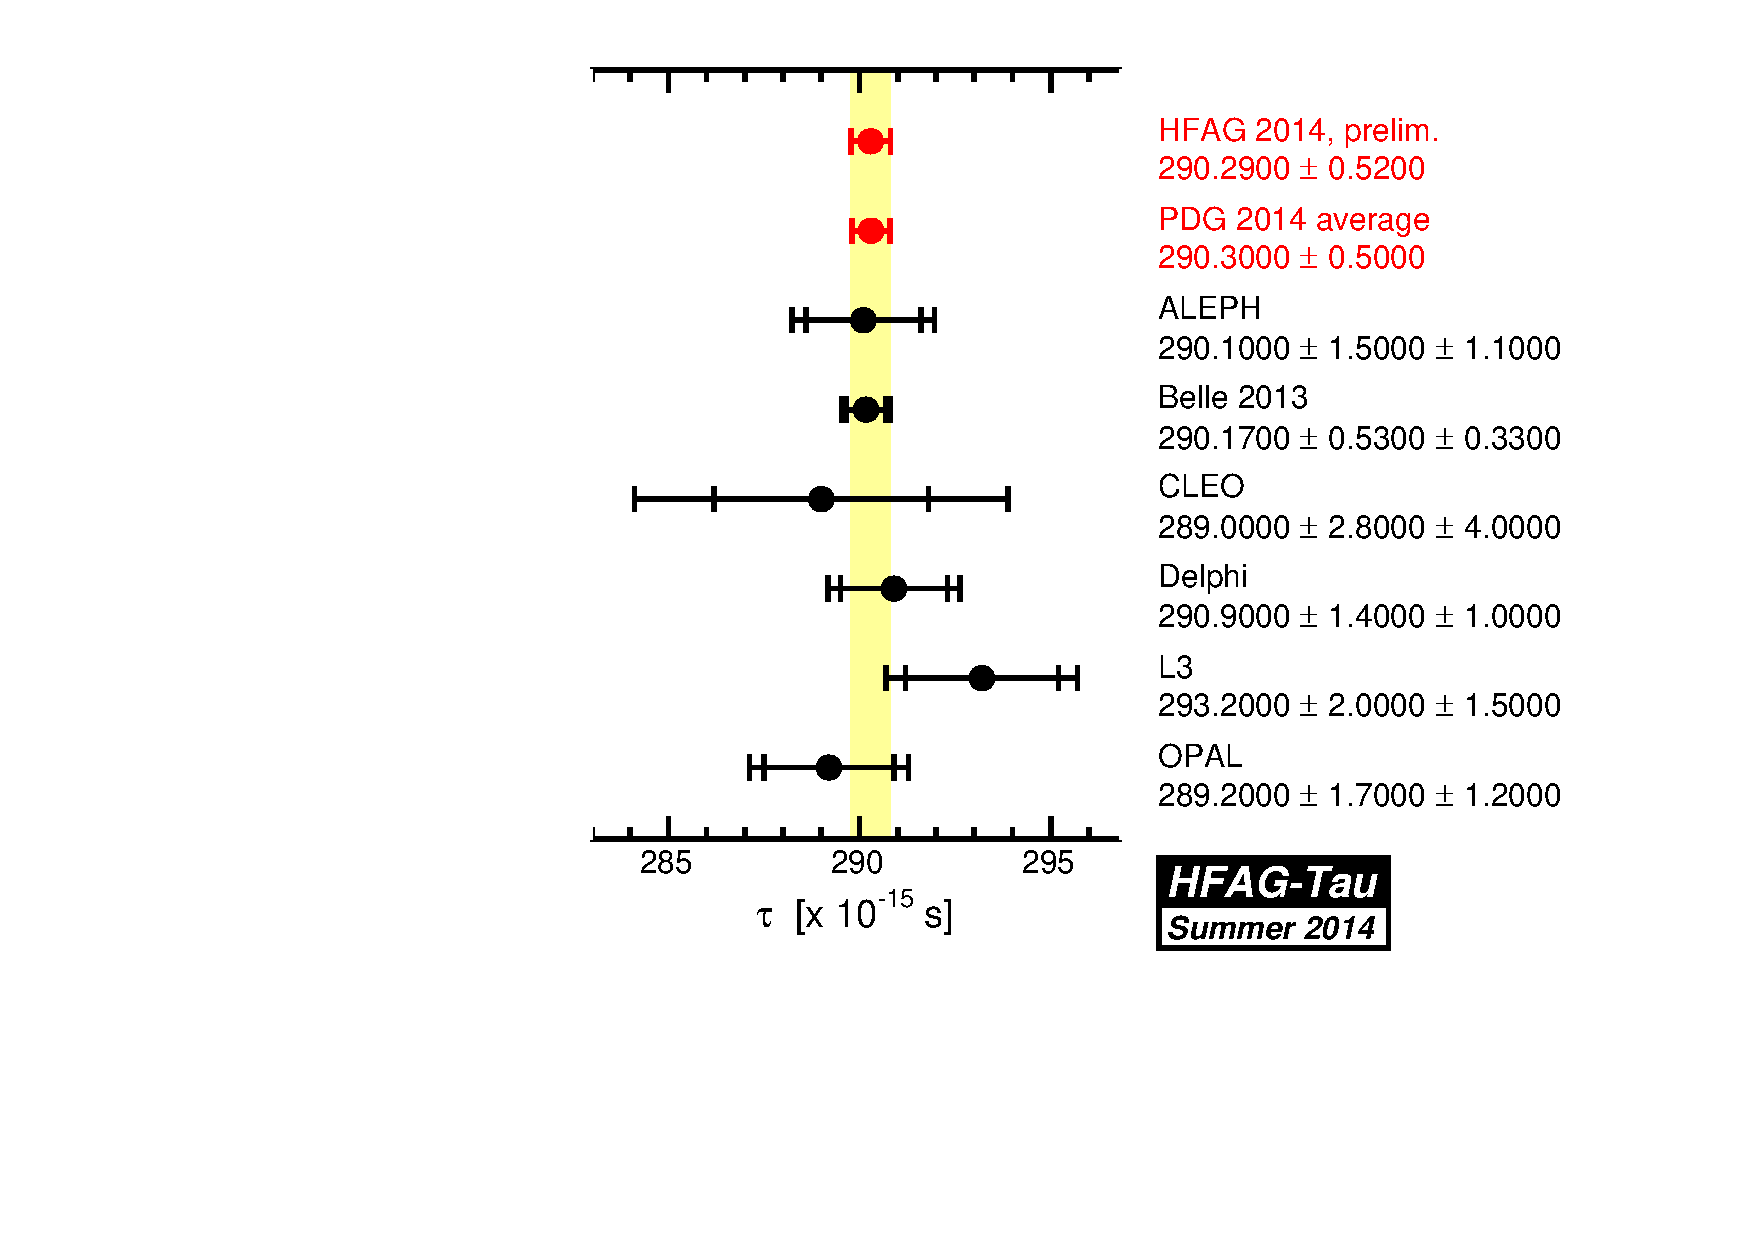
\includegraphics[width=0.75\linewidth,clip]{figures/tau/plot-taulife-hfag-summer2014.pdf}
    \fi
    \caption{\mtau lifetime average.%
      \label{fig:tau:tau-lifetime}%
    }
  \end{center}
\end{figure}

%% ///////////////////////////////////////////////////////////////////////////
\tausection{Tests of lepton universality}
\cutname{lepton-univ.html}
\label{sec:tau:leptonuniv}

Lepton universality tests precision has been significantly improved by the
addition of the recent Belle \mtau lifetime
measurement~\cite{Belous:2013dba}, while improvements from the \mtau
branching fraction fit are negligible.
We compute the universality tests like in the previous report by using
proper ratios of the partial widths of a heavier lepton \lepth
decaying to a
lighter lepton \leptl~\cite{Marciano:1988vm},
\begin{align*}
  \Gamma(\lepth \to \nu_{\lepth} \leptl \nub_{\leptl} (\gamma)) =
  \frac{\BR(\lepth \to \nu_{\lepth} \leptl \nub_{\leptl})}{\tau_{\lepth}} =
  \frac {G_{\lepth} G_{\leptl} m^5_{\lepth}}{192 \pi^3}\, f\left(\frac {m^2_{\leptl}}{m^2_{\lepth}}\right)
  \opdelta^{\lepth}_W \opdelta^{\lepth}_\gamma~,
\end{align*}
where
\begin{alignat*}{3}
 G_{\leptl} &= \frac {g^2_{\leptl}}{4 \sqrt{2} M^2_W}~, &\quad&&
 f(x) &= 1 -8x +8x^3 -x^4 -12x^2 \text{ln}x~, \\
 \opdelta^{\lepth}_W &= 1 + \frac {3}{5} \frac {m^2_{\lepth}}{M^2_W}~, &\quad\quad&&
 \opdelta^{\lepth}_\gamma &= 1+\frac {\alpha(m_{\lepth})}{2\pi} \left(\frac {25}{4}-\pi^2\right)~.
\end{alignat*}
We use $\opdelta^\tau_\gamma=1-43.2\cdot 10^{-4}$ and
$\opdelta^\mu_\gamma=1-42.4\cdot 10^{-4}$~\cite{Marciano:1988vm} and $M_W$
from PDG 2013~\cite{PDG_2012}.
We use HFAG 2014 averages and PDG 2013 for the other quantities.
Using pure leptonic processes we obtain
\begin{align*}
  \left( \frac{g_\tau}{g_\mu} \right) = \htuse{gtaubygmu_tau}~,
  && \left( \frac{g_\tau}{g_e} \right) = \htuse{gtaubyge_tau}~,
  && \left( \frac{g_\mu}{g_e} \right) = \htuse{gmubyge_tau}~.
\end{align*}
Using semi-hadronic processes
\begin{align*}
  \left( \frac{g_\tau}{g_\mu} \right)^2 =
  \frac{\BR({\tau \to h \nu_\tau})}{\BR({h \to \mu \bar{\nu}_\mu})}
  \frac{2m_h m^2_{\mu}\tau_h}{(1+\delta_{h})m^3_{\tau}\tau_{\tau}}
  \left( \frac{1-m^2_{\mu}/m^2_h}{1-m^2_h/m^2_{\tau}} \right)^2~,
\end{align*}
where $h$ = $\pi$ or $K$ and the radiative corrections are
$\delta_{\pi} = (\htuse{delta_LD_taupi_pimu})\%$ and
$\delta_{K} = (\htuse{delta_LD_tauK_Kmu})\%$~\cite{Decker:1994dd}.
we measure:
\begin{align*}
  \left( \frac{g_\tau}{g_\mu} \right)_\pi &= \htuse{gtaubygmu_pi}~,
  & \left( \frac{g_\tau}{g_\mu} \right)_K = \htuse{gtaubygmu_K}~.
\end{align*}
Similar tests could be performed with decays to electrons, however they are
less precise because the hadron two body decays to electrons are
helicity-suppressed.
Averaging the three \(g_\tau/g_\mu\) ratios we obtain
\begin{align*}
  \left( \frac{g_\tau}{g_\mu} \right)_{\tau{+}\pi{+}K} &= \htuse{gtaubygmu_fit}~,
\end{align*}
accounting for statistical correlations.
Table~\ref{tab:tau:univ-fit-corr} reports the statistical correlation coefficients for the fitted coupling ratios:
\ifhevea\begin{table}\fi%% otherwise cannot have normalsize caption
\begin{center}
\ifhevea
\caption{Universality coupling ratios correlation coefficients (\%).\label{tab:tau:univ-fit-corr}}%
\else
\begin{minipage}{\linewidth}
\begin{center}
\captionof{table}{Universality coupling ratios correlation coefficients (\%).}\label{tab:tau:univ-fit-corr}%
\fi
\begin{center}
\renewcommand*{\arraystretch}{1.1}%
\begin{tabular}{lcccc}
\toprule
\htuse{couplingsCorr}
\\\bottomrule
\end{tabular}
\end{center}
\ifhevea\else
\end{center}
\end{minipage}
\fi
\end{center}
\ifhevea\end{table}\fi

%% ///////////////////////////////////////////////////////////////////////////
\tausection{Universality improved $\BR(\tau \to e \nu \bar{\nu})$ and $\Rhad$}
\cutname{Be_univ_and_Rtau.html}
\label{sec:tau:be-univ-rtau}

Following Ref.~\cite{Davier:2005xq}, we assume lepton universality to
obtain a more precise experimental determination of $\BR_e = \BR(\tau \to
e\bar{\nu}_e\nu_\tau)$ using the \mtau branching fraction to muon and the \mtau
lifetime. We average:
\begin{itemize}

\item the $\BR_e$ fit value,

\item the $\BR_e$ determination from $\BR_\mu$ assuming that
$g_\mu/g_e = 1$ hence (see also Section~\ref{sec:tau:leptonuniv})
$\BR_e = \BR_\mu \cdot f(m^2_e/m^2_\tau)/f(m^2_\mu/m^2_\tau)$,

\item the $\BR_e$ determination from the \mtau lifetime assuming that
$g_\tau/g_\mu =1$ hence $\BR_e = \BR(\mu \to e \bar{\nu}_e
\nu_\mu)\cdot (\tau_\tau / \tau_\mu) \cdot (m_\tau/m_\mu)^5 \cdot
f(m^2_e/m^2_\tau)/f(m^2_e/m^2_\mu) \cdot (\delta_\gamma^\tau
\delta_W^\tau)/(\delta_\gamma^\mu \delta_W^\mu)$ where $\BR(\mu \to e
\bar{\nu}_e \nu_\mu) = 1$.

\end{itemize}
Accounting for statistical correlations, we obtain
\begin{align*}
  \BR_e^{\text{uni}} = (\htuse{Be_univ})\%.
\end{align*}
The recent Belle \mtau lifetime measurement has brought a significant improvement.
We use $\BR_e^{\text{uni}}$ to obtain the ratio
\begin{align*}
  \Rhad = \frac{\Gamma(\tau \to \text{hadrons})}{\Gamma(\tau\to e\nu\bar{\nu})} = \htuse{R_tau}.
\end{align*}
Here $\Gamma(\tau \to \text{hadrons})$ is obtained by summing all \mtau
hadronic decay modes.

%% ///////////////////////////////////////////////////////////////////////////
\tausection{$\Vus$ measurement}
\cutname{vus.html}
\label{sec:tau:vus}

We have updated the CKM coefficient \Vus determinations of the previous
report using the updated data from HFAG 2014 and PDG 2013.

\tausubsection{Inclusive \mtau partial width to strange}

The \mtau hadronic partial width is the sum of the \mtau partial width to
strange and to non-strange hadronic final states,
$\Gammahad = \Gammastrange + \Gammanonstrange$.
Dividing by the partial width to electron, $\Gamma_e$, we obtain partial width ratios
(which are equal to the respective branching fraction ratios) for which
$\Rhad =  \Rstrange + \Rnonstrange$. In terms
of such ratios, \Vus is measured as~\cite{Gamiz:2006xx}
\begin{align*}
  \VusTauIncl &= \sqrt{\Rstrange/\left[\frac{\Rnonstrange}{\Vud^2} -  \delta R_{\text{theory}}\right]}~,
\end{align*}
where $\delta R_{\text{theory}}$ can be determined in the context of low
energy QCD theory, partly relying on experimental low energy scattering
data. The literature reports several
calculations~\cite{Gamiz:2006xx,Gamiz:2007qs,Maltman:2010hb}. In this
report we use Ref.~\cite{Gamiz:2006xx}, whose estimated uncertainty size is
in between the two other ones. We use the information in that paper and the
PDG 2013 value for the $s$-quark mass $m_s = \htuse{m_s}$~\cite{PDG_2012}
to calculate $\delta R_{\text{theory}} = \htuse{deltaR_su3break}$.

We proceed following the same procedure of the 2012 HFAG
report~\cite{Amhis:2012bh}, using the universality improved $\BR_e^{\text{uni}}$
(see Section~\ref{sec:tau:be-univ-rtau}) to compute the $R$ ratios, and
using the sum of the \mtau branching fractions to strange and
non-strange hadronic final states to compute \Rstrange and \Rnonstrange,
respectively.

Using the \mtau branching fraction fit results with their uncertainties
and correlations (Section~\ref{sec:tau:br-fit}), we compute $\BRstrange =
(\htuse{B_tau_s_fit})\%$ (see also Table~\ref{tab:tau:vus}) and
$\BRnonstrange = (\htuse{B_tau_VA_fit})\%$. PDG 2013 averages
are used for non-\mtau quantities, including $\Vud = \htuse{Vud}$, which
comes from Ref.~\cite{Hardy:2008gy} like for the previous HFAG report.

We obtain $\VusTauIncl = \htuse{Vus}$, which
is $\htuse{Vus_mism_sigma_abs}\sigma$ lower than the unitarity CKM
prediction $\VusUni = \htuse{Vus_uni}$, from $(\VusUni)^2 = 1 -
\Vud^2$. The \VusTauIncl uncertainty includes a systematic error
contribution of \htuse{Vus_err_th_perc}\% from the theory uncertainty on
$\delta R_{\text{theory}}$. There is no significant change with respect to
the previous HFAG report.

Kim Maltman has computed an alternative theoretical estimate based on Fixed
Order Pertubation Theory and experimental inputs restricted to \mtau
quantities. 
The result is  $\delta R_{\text{theory}} = 0.254 \pm 0.038$~\cite{Maltman:oct2014}.
The uncertainty includes an additional contribution to account
for the differences between using Fixed Order Pertubation Theory and Contour
Improved Perturbation Theory. With this alternative value, we would obtain
$\VusTauIncl = 0.2181 \pm 0.0022$, which would be $3.1\sigma$ lower than
the unitarity CKM prediction.

%%
%% Gamma110 quantities
%%
\begin{table}
\begin{center}
\renewcommand*{\arraystretch}{1.3}%
\caption{HFAG \hfagTauTag \mtau branching fractions to strange final states.\label{tab:tau:vus}}%
\ifhevea\renewcommand{\bar}[1]{\textoverline{#1}}\fi
\begin{envsmall}
\begin{center}
\begin{tabular}{llll}
\hline
\multicolumn{1}{c}{\bfseries Branching fraction} &
\multicolumn{1}{c}{\bfseries HFAG \hfagTauTag fit} \\
\hline
\htuse{BrStrangeVal}
\\\hline
\htuse{BrStrangeTotVal}
\\\hline
\end{tabular}
\end{center}
\end{envsmall}
\end{center}
\end{table}

\tausubsection{\Vus from $\BR(\tau \to K\nu) / \BR(\tau \to \pi\nu)$ and from $\BR(\tau \to K\nu)$}

We follow the same procedure of the HFAG 2012 report to compute \Vus from
the ratio of branching fractions $\BFtautoknu/\BFtautopinu =
\htuse{Gamma10by5}$ from the equation
\begin{align*}
\frac{\BFtautoknu}{\BFtautopinu} &=
\frac{f_K^2 \Vus^2}{f_\pi^2 \Vud^2} \frac{\left( 1 - m_K^2/m_\tau^2 \right)^2}{\left( 1 -  m_\pi^2/m_\tau^2 \right)^2}
\frac{\opdelta_{\text{LD}}(\tau^- \to K^-\nut)}{\opdelta_{\text{LD}}(\tau^- \to \pi^-\nut)}~.
\end{align*}
We use $f_K/f_\pi = \htuse{f_K_by_f_pi}$ from the
FLAG 2013 Lattice averages with $N_f=2+1$~\cite{Aoki:2013ldr}.
We compute $\VusTauKpi = \htuse{Vus_tauKpi}$,
$\htuse{Vus_tauKpi_mism_sigma_abs}\sigma$ below the CKM unitarity prediction.

We proceed like in 2012 also to determine \Vus from the branching fraction
$\BFtautoknu$ using
\begin{align*}
  \BR(\tau^- \to K^-\nu_\tau) =
  \frac{G^2_F f^2_K \Vus^2 m^3_{\tau} \tau_{\tau}}{16\pi\hbar} \left (1 - \frac{m_K^2}{m_\tau^2} \right )^2 S_{EW}~.
\end{align*}
We use $f_K = \htuse{f_K}\,\mev$ from FLAG 2013 with
$N_f=2+1$~\cite{Aoki:2013ldr}. We obtain $\VusTauKnu = \htuse{Vus_tauKnu}$,
which is $\htuse{Vus_tauKnu_mism_sigma_abs}\sigma$ below
the CKM unitarity prediction. CODATA 2010 results~\cite{Mohr:2012tt} and
PDG 2013 have been used for the physics constants.

\tausubsection{\Vus from \mtau summary}

\begin{figure}[tb]
  \begin{center}
   \ifhevea
    \begin{tabular}{@{}cc@{}}
      \larger\bfseries\ahref{hfag-tau-vus-plot.png}{PNG format} &
      \larger\bfseries\ahref{hfag-tau-vus-plot.pdf}{PDF format} \\
      \multicolumn{2}{c}{\ahref{hfag-tau-vus-plot.png}{%
          \imgsrc[alt="Vus summary plot"]{hfag-tau-vus-plot.png}}}
    \end{tabular}
    \else
    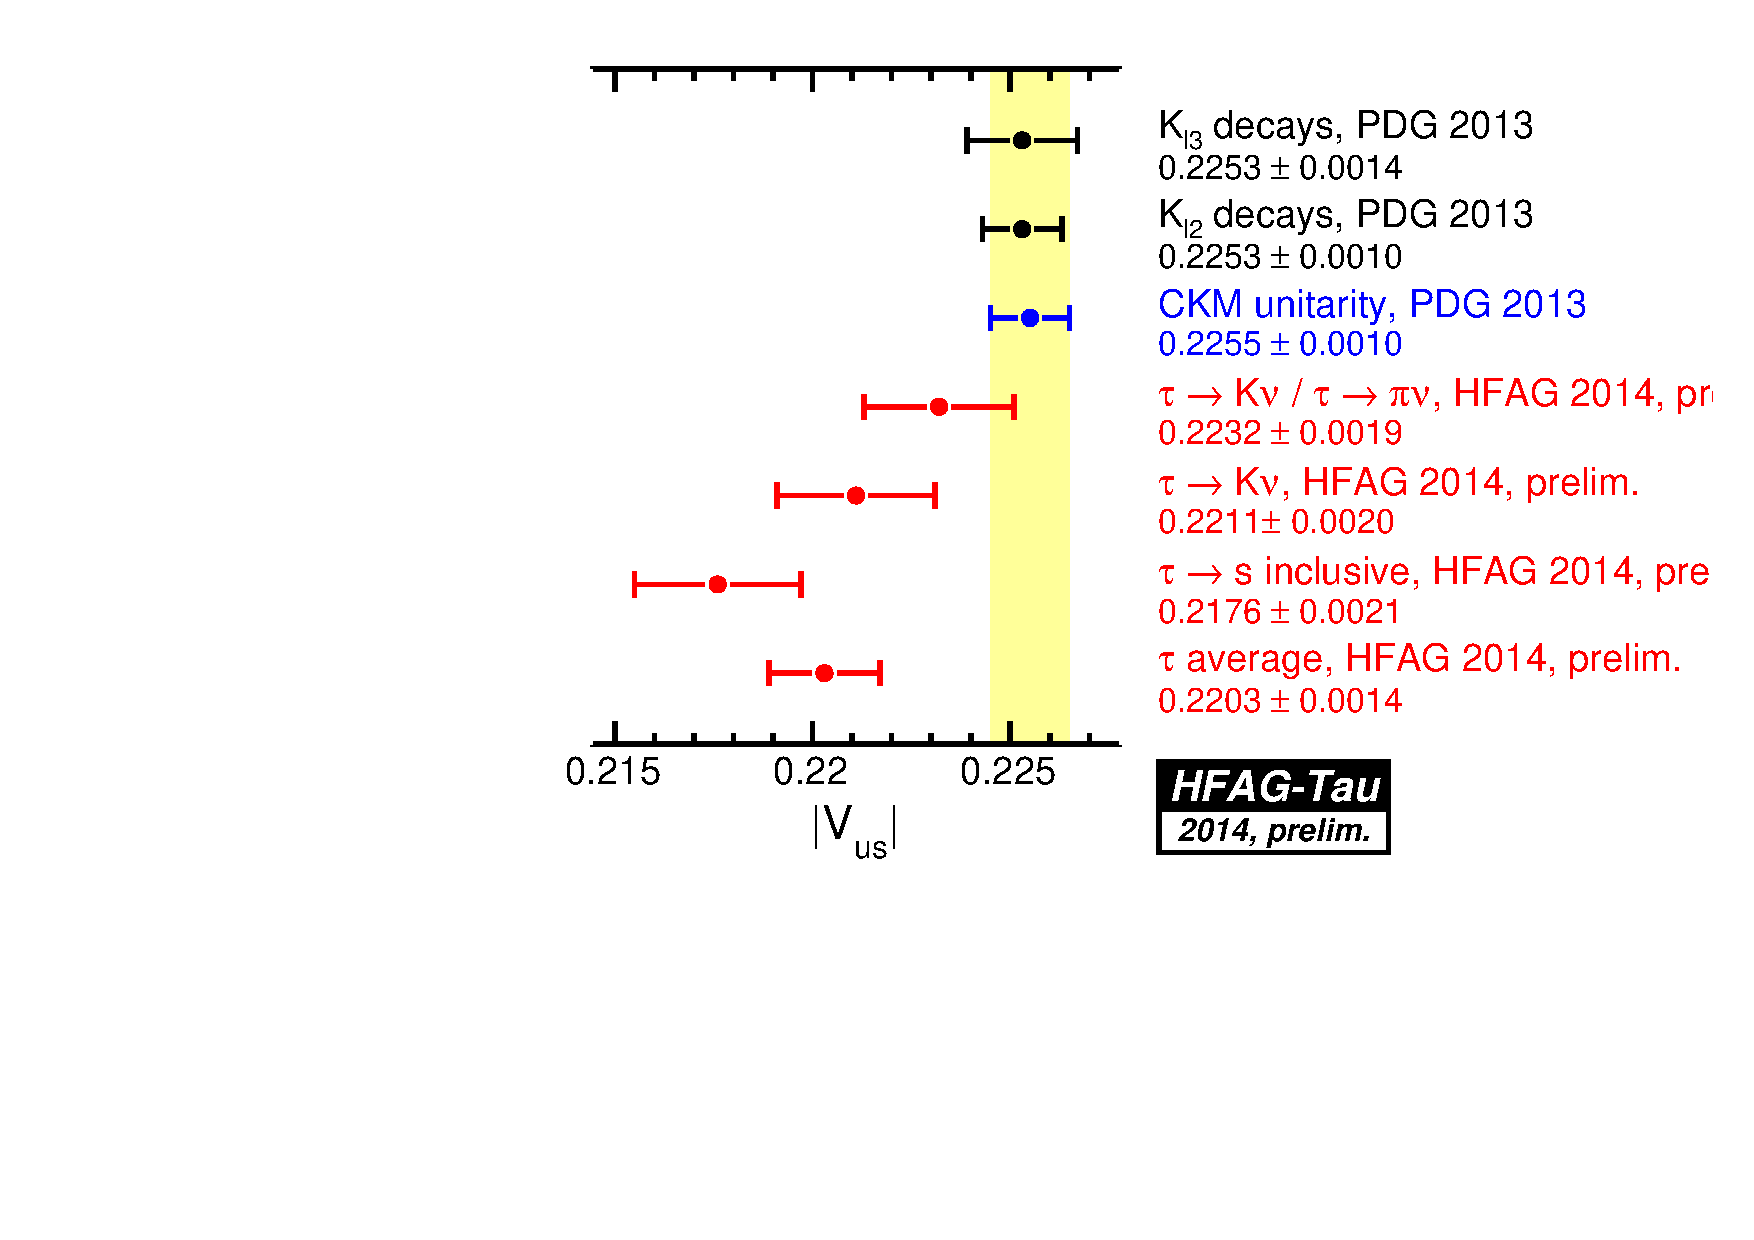
\includegraphics[width=0.75\linewidth,clip]{figures/tau/hfag-tau-vus-plot.pdf}
    \fi
    \caption{\Vus averages of this document compared with the FlaviaNet results~\cite{Antonelli:2010yf}.
      \label{fig:tau:vus-summary}%
    }
  \end{center}
\end{figure}

We summarize the \Vus results reporting the values, the discrepancy with
respect to the \Vus determination from CKM unitarity, and an illustration
of the measurement method:
\begin{alignat*}{6}
  &\VusUni &&= \htuse{Vus_uni.v} &&\pm \htuse{Vus_uni.e} & \quad & & \quad
  & {\smaller\text{from } \sqrt{1 - \Vud^2} \quad\text{(CKM unitarity)}}~, \\
  %%
  &\VusTauIncl &&= \htuse{Vus.v} &&\pm \htuse{Vus.e} & \quad & \htuse{Vus_mism_sigma}\sigma &
  & {\smaller\text{from } \Gamma(\tau^- \to X_s^- \nut)}~, \\
  %%
  &\VusTauKpi &&= \htuse{Vus_tauKpi.v} &&\pm \htuse{Vus_tauKpi.e} & \quad & \htuse{Vus_tauKpi_mism_sigma}\sigma &
  & {\smaller\text{from } \Gamma(\tauknu)/\Gamma(\taupinu)}~,  \\
  %%
  &\VusTauKnu &&= \htuse{Vus_tauKnu.v} &&\pm \htuse{Vus_tauKnu.e} & \quad & \htuse{Vus_tauKnu_mism_sigma}\sigma &
  & {\smaller\text{from } \Gamma(\tauknu)}~.
\end{alignat*}

Averaging the three above \Vus determinations (taking into account all
correlations due to the usage of the fitted \mtau branching fractions and
the other mentioned inputs) we obtain:
\begin{alignat*}{6}
  & \Vus_\tau &&= \htuse{Vus_tau} &\quad &\htuse{Vus_tau_mism_sigma}\sigma \quad
  & \text{average of 3 \Vus \mtau measurements}.
\end{alignat*}
We could not find a published estimate of the correlation of the
uncertainties on $f_K$ and $f_K/f_\pi$, but even if we assume $\pm
100\%$ correlation, the uncertainty on $\Vus_\tau$ does not change
more than about $\pm 5\%$. Figure~\ref{fig:tau:vus-summary} summarizes the
\Vus results.

%% -*- mode: LaTeX; TeX-master: "../Summer14.tex" -*-
\tausection{Upper limits on \mtau LFV branching fractions}
\cutname{lfv-limits.html}
\label{sec:tau:lfv}
We report in Table~\ref{tab:tau:lfv-upper-limits} the up-to-date upper
limits on the \mtau LFV branching fractions.
\begin{center}
\begin{longtable}{lcl@{}rll}
\caption{Experimental upper limits on lepton flavor violating \mtau
  decays. The modes are grouped according to the particle content of their final
  states. Modes with lepton number violation are labeled with ``(L)'',
  modes with baryon number violation are labeled with ``(BNV)''.
  \label{tab:tau:lfv-upper-limits}}%
\\
\toprule
\multicolumn{1}{l}{\bfseries Decay mode} &
\multicolumn{1}{l}{\bfseries Category} &
\multicolumn{2}{c}{\bfseries \begin{tabular}{@{}c@{}}90\% CL\\Limit\end{tabular}} &
\multicolumn{1}{l}{\bfseries Exp.} &
\multicolumn{1}{l}{\bfseries Ref.} \\
\midrule
\endfirsthead
\multicolumn{6}{c}{{\bfseries \tablename\ \thetable{} -- continued from previous page}} \\ \midrule
\multicolumn{1}{l}{\bfseries Decay mode} &
\multicolumn{1}{l}{\bfseries Category} &
\multicolumn{2}{c}{\bfseries \begin{tabular}{@{}c@{}}90\% CL\\Limit\end{tabular}} &
\multicolumn{1}{l}{\bfseries Exp.} &
\multicolumn{1}{l}{\bfseries Ref.} \\
\midrule
\endhead
%
%  l\gamma
%   
\begin{ensuredisplaymath}
\Gamma_{156} =  {e^- \gamma} 
\end{ensuredisplaymath}
 &\(l\gamma\) & \( <\; \) & \(12.0 \cdot 10^{-8}\)         & Belle &  \cite{Hayasaka:2007vc} \\
 &            & \( <\; \) & \(3.3 \cdot 10^{-8}\)         & \babar &  \cite{Aubert:2009ag}   \\ 
%\midrule
\begin{ensuredisplaymath}
\Gamma_{157} =  {\mu^- \gamma} 
\end{ensuredisplaymath}
 &            & \( <\; \) & \(4.5 \cdot 10^{-8}\)         & Belle &  \cite{Hayasaka:2007vc} \\
 &            & \( <\; \) & \(4.4 \cdot 10^{-8}\)         & \babar &  \cite{Aubert:2009ag}   \\ 
\midrule
%
%  lP0
% 
\begin{ensuredisplaymath}
\Gamma_{158} =  {e^- \pi^0} 
\end{ensuredisplaymath}
 &\(lP^0 \)   & \( <\; \) & \(2.2 \cdot 10^{-8}\)         & Belle & \cite{Hayasaka:2011zz} \\
 &            & \( <\; \) & \(13.0 \cdot 10^{-8}\)         & \babar & \cite{Aubert:2006cz} \\ 
%\midrule
\begin{ensuredisplaymath}
\Gamma_{159} =  {\mu^- \pi^0} 
\end{ensuredisplaymath}
 &            & \( <\; \) & \(2.7 \cdot 10^{-8}\)         & Belle &  \cite{Hayasaka:2011zz}  \\
 &            & \( <\; \) & \(11.0 \cdot 10^{-8}\)         & \babar &  \cite{Aubert:2006cz} \\ 
%\midrule
\begin{ensuredisplaymath}
\Gamma_{162} =  {e^- \eta} 
\end{ensuredisplaymath}
 &            & \( <\; \) & \(4.4 \cdot 10^{-8}\)         & Belle &  \cite{Hayasaka:2011zz}  \\
 &            & \( <\; \) & \(16.0 \cdot 10^{-8}\)         & \babar &  \cite{Aubert:2006cz} \\ 
%\midrule
\begin{ensuredisplaymath}
\Gamma_{163} =  {\mu^- \eta} 
\end{ensuredisplaymath}
 &            & \( <\; \) & \(2.3 \cdot 10^{-8}\)         & Belle &   \cite{Hayasaka:2011zz} \\
 &            & \( <\; \) & \(15.0 \cdot 10^{-8}\)         & \babar &   \cite{Aubert:2006cz} \\ 
%\midrule
\begin{ensuredisplaymath}
\Gamma_{172} =  {e^- \eta'(958)} 
\end{ensuredisplaymath}
 &            & \( <\; \) & \(3.6 \cdot 10^{-8}\)         & Belle &   \cite{Hayasaka:2011zz}  \\
 &            & \( <\; \) & \(24.0 \cdot 10^{-8}\)         & \babar &   \cite{Aubert:2006cz} \\ 
%\midrule
\begin{ensuredisplaymath}
\Gamma_{173} =  {\mu^- \eta'(958)} 
\end{ensuredisplaymath}
 &            & \( <\; \) & \(3.8 \cdot 10^{-8}\)         & Belle &   \cite{Hayasaka:2011zz}  \\
 &            & \( <\; \) & \(14.0 \cdot 10^{-8}\)         & \babar &   \cite{Aubert:2006cz} \\ 
%\midrule
\begin{ensuredisplaymath}
\Gamma_{160} =  {e^- K^0_S} 
\end{ensuredisplaymath}
 &            & \( <\; \) & \(2.6 \cdot 10^{-8}\)         & Belle &  \cite{Miyazaki:2010qb} \\
 &            & \( <\; \) & \(3.3 \cdot 10^{-8}\)         & \babar &  \cite{Aubert:2009ys}   \\ 
%\midrule
\begin{ensuredisplaymath}
\Gamma_{161} =  {\mu^- K^0_S} 
\end{ensuredisplaymath}
 &            & \( <\; \) & \(2.3 \cdot 10^{-8}\)         & Belle &   \cite{Miyazaki:2010qb} \\
 &            & \( <\; \) & \(4.0 \cdot 10^{-8}\)         & \babar &   \cite{Aubert:2009ys}   \\ 
\midrule
%
%  l S^0
%
\begin{ensuredisplaymath}
\Gamma_{174} =  {e^- f_0(980)} 
\end{ensuredisplaymath}
 &  \(l S^0\) & \( <\; \) & \(3.2 \cdot 10^{-8}\)         & Belle & \cite{Miyazaki:2008mw}\\
%&            & \( <\; \) & \(1.0 \cdot 10^{-8}\)         & \babar &                       \\ 
%\midrule
\begin{ensuredisplaymath}
\Gamma_{175} =  {\mu^- f_0(980)} 
\end{ensuredisplaymath}
 &            & \( <\; \) & \(3.4 \cdot 10^{-8}\)         & Belle & \cite{Miyazaki:2008mw}\\  
%&            & \( <\; \) & \(1.0 \cdot 10^{-8}\)         & \babar &                       \\ 
\midrule
%
% l V0
%
\begin{ensuredisplaymath}
\Gamma_{164} =  {e^- \rho^0} 
\end{ensuredisplaymath}
 &  \(l V^0\) & \( <\; \) & \(1.8 \cdot 10^{-8}\)         & Belle &  \cite{Miyazaki:2011xe}\\
 &            & \( <\; \) & \(4.6 \cdot 10^{-8}\)         & \babar &  \cite{Aubert:2009ap}  \\ 
%\midrule
\begin{ensuredisplaymath}
\Gamma_{165} =  {\mu^- \rho^0} 
\end{ensuredisplaymath}
 &            & \( <\; \) & \(1.2 \cdot 10^{-8}\)         & Belle &  \cite{Miyazaki:2011xe}\\
 &            & \( <\; \) & \(2.6 \cdot 10^{-8}\)         & \babar &  \cite{Aubert:2009ap}  \\ 
%\midrule
\begin{ensuredisplaymath}
\Gamma_{168} =  {e^- K^*(892)^0} 
\end{ensuredisplaymath}
 &            & \( <\; \) & \(3.2 \cdot 10^{-8}\)         & Belle &  \cite{Miyazaki:2011xe} \\
 &            & \( <\; \) & \(5.9 \cdot 10^{-8}\)         & \babar &  \cite{Aubert:2009ap}   \\ 
%\midrule
\begin{ensuredisplaymath}
\Gamma_{169} =  {\mu^- K^*(892)^0} 
\end{ensuredisplaymath}
 &            & \( <\; \) & \(7.2 \cdot 10^{-8}\)         & Belle &   \cite{Miyazaki:2011xe} \\
 &            & \( <\; \) & \(17.0 \cdot 10^{-8}\)         & \babar &   \cite{Aubert:2009ap}   \\ 
%\midrule
\begin{ensuredisplaymath}
\Gamma_{170} =  {e^- \bar{K}^*(892)^0} 
\end{ensuredisplaymath}
 &            & \( <\; \) & \(3.4 \cdot 10^{-8}\)         & Belle &   \cite{Miyazaki:2011xe} \\
 &            & \( <\; \) & \(4.6 \cdot 10^{-8}\)         & \babar &   \cite{Aubert:2009ap}   \\ 
%\midrule
\begin{ensuredisplaymath}
\Gamma_{171} =  {\mu^- \bar{K}^*(892)^0} 
\end{ensuredisplaymath}
 &            & \( <\; \) & \(7.0 \cdot 10^{-8}\)         & Belle &  \cite{Miyazaki:2011xe} \\
 &            & \( <\; \) & \(7.3 \cdot 10^{-8}\)         & \babar &  \cite{Aubert:2009ap}   \\ 
%\midrule

\begin{ensuredisplaymath}
\Gamma_{176} =  {e^- \phi} 
\end{ensuredisplaymath}
 &            & \( <\; \) & \(3.1 \cdot 10^{-8}\)         & Belle &   \cite{Miyazaki:2011xe} \\
 &            & \( <\; \) & \(3.1 \cdot 10^{-8}\)         & \babar &   \cite{Aubert:2009ap}   \\ 
%\midrule
\begin{ensuredisplaymath}
\Gamma_{177} =  {\mu^- \phi} 
\end{ensuredisplaymath}
 &            & \( <\; \) & \(8.4 \cdot 10^{-8}\)         & Belle &   \cite{Miyazaki:2011xe} \\
 &            & \( <\; \) & \(19.0 \cdot 10^{-8}\)         & \babar &   \cite{Aubert:2009ap}   \\ 
%\midrule
\begin{ensuredisplaymath}
\Gamma_{166} =  {e^- \omega} 
\end{ensuredisplaymath}
 &            & \( <\; \) & \(4.8 \cdot 10^{-8}\)         & Belle &  \cite{Miyazaki:2011xe} \\
 &            & \( <\; \) & \(11.0 \cdot 10^{-8}\)         & \babar &  \cite{Aubert:2007kx}   \\ 
%\midrule
\begin{ensuredisplaymath}
\Gamma_{167} =  {\mu^- \omega} 
\end{ensuredisplaymath}
 &            & \( <\; \) & \(4.7 \cdot 10^{-8}\)         & Belle &  \cite{Miyazaki:2011xe} \\
 &            & \( <\; \) & \(10.0 \cdot 10^{-8}\)         & \babar &  \cite{Aubert:2007kx}   \\ 
\midrule
%
% lll
%
\begin{ensuredisplaymath}
\Gamma_{178} =  {e^- e^+ e^-} 
\end{ensuredisplaymath}
 &  \(lll\)   & \( <\; \) & \(2.7 \cdot 10^{-8}\)         & Belle & \cite{Hayasaka:2010np} \\
 &            & \( <\; \) & \(2.9 \cdot 10^{-8}\)         & \babar & \cite{Lees:2010ez}     \\ 
%\midrule
\begin{ensuredisplaymath}
\Gamma_{181} =  {\mu^- e^+ e^-} 
\end{ensuredisplaymath}
 &            & \( <\; \) & \(1.8 \cdot 10^{-8}\)         & Belle & \cite{Hayasaka:2010np} \\
 &            & \( <\; \) & \(2.2 \cdot 10^{-8}\)         & \babar & \cite{Lees:2010ez}     \\ 
%\midrule
\begin{ensuredisplaymath}
\Gamma_{179} =  {e^- \mu^+ \mu^-} 
\end{ensuredisplaymath}
 &            & \( <\; \) & \(2.7 \cdot 10^{-8}\)         & Belle & \cite{Hayasaka:2010np} \\
 &            & \( <\; \) & \(3.2 \cdot 10^{-8}\)         & \babar & \cite{Lees:2010ez}     \\ 
%\midrule
\begin{ensuredisplaymath}
\Gamma_{183} =  {\mu^- \mu^+ \mu^-} 
\end{ensuredisplaymath}
 &            & \( <\; \) & \(2.1 \cdot 10^{-8}\)         & Belle & \cite{Hayasaka:2010np} \\
 &            & \( <\; \) & \(3.3 \cdot 10^{-8}\)         & \babar &
  \cite{Lees:2010ez}     \\ 
 &            & \( <\; \) & \(4.6 \cdot 10^{-8}\)         & \lhcb &
  \cite{Aaij:2014azz}     \\ 

%\midrule
\begin{ensuredisplaymath}
\Gamma_{182} =  {e^- \mu^+ e^-} 
\end{ensuredisplaymath}
 &            & \( <\; \) & \(1.5 \cdot 10^{-8}\)         & Belle & \cite{Hayasaka:2010np} \\
 &            & \( <\; \) & \(1.8 \cdot 10^{-8}\)         & \babar & \cite{Lees:2010ez}     \\ 
%\midrule
\begin{ensuredisplaymath}
\Gamma_{180} =  {\mu^- e^+ \mu^-} 
\end{ensuredisplaymath}
 &            & \( <\; \) & \(1.7 \cdot 10^{-8}\)         & Belle & \cite{Hayasaka:2010np} \\
 &            & \( <\; \) & \(2.6 \cdot 10^{-8}\)         & \babar & \cite{Lees:2010ez}     \\ 
\midrule
%
% l h h
%
\begin{ensuredisplaymath}
\Gamma_{184} =  {e^- \pi^+ \pi^-} 
\end{ensuredisplaymath}
 &    \(lhh\) & \( <\; \) & \(2.3 \cdot 10^{-8}\)         & Belle &  \cite{Miyazaki:2012mx}\\
 &            & \( <\; \) & \(12.0 \cdot 10^{-8}\)         & \babar &  \cite{Aubert:2005tp}  \\ 
%\midrule
\begin{ensuredisplaymath}
\Gamma_{186} =  {\mu^- \pi^+  \pi^-} 
\end{ensuredisplaymath}
 &            & \( <\; \) & \(2.1 \cdot 10^{-8}\)         & Belle &  \cite{Miyazaki:2012mx} \\
 &            & \( <\; \) & \(29.0 \cdot 10^{-8}\)         & \babar &  \cite{Aubert:2005tp}   \\ 
%\midrule
\begin{ensuredisplaymath}
\Gamma_{188} =  {e^- \pi^+ K^-} 
\end{ensuredisplaymath}
 &            & \( <\; \) & \(3.7 \cdot 10^{-8}\)         & Belle &  \cite{Miyazaki:2012mx} \\
 &            & \( <\; \) & \(32.0 \cdot 10^{-8}\)         & \babar &  \cite{Aubert:2005tp}   \\ 
%\midrule
\begin{ensuredisplaymath}
\Gamma_{194} =  {\mu^- \pi^+  K^-} 
\end{ensuredisplaymath}
 &            & \( <\; \) & \(8.6 \cdot 10^{-8}\)         & Belle &   \cite{Miyazaki:2012mx} \\
 &            & \( <\; \) & \(26.0 \cdot 10^{-8}\)         & \babar &   \cite{Aubert:2005tp}   \\ 
%\midrule
\begin{ensuredisplaymath}
\Gamma_{189} =  {e^- K^+ \pi^-} 
\end{ensuredisplaymath}
 &            & \( <\; \) & \(3.1 \cdot 10^{-8}\)         & Belle &   \cite{Miyazaki:2012mx} \\
 &            & \( <\; \) & \(17.0 \cdot 10^{-8}\)         & \babar &   \cite{Aubert:2005tp}   \\ 
%\midrule
\begin{ensuredisplaymath}
\Gamma_{195} =  {\mu^- K^+  \pi^-} 
\end{ensuredisplaymath}
 &            & \( <\; \) & \(4.5 \cdot 10^{-8}\)         & Belle &   \cite{Miyazaki:2012mx} \\
 &            & \( <\; \) & \(32.0 \cdot 10^{-8}\)         & \babar &   \cite{Aubert:2005tp}   \\ 
%\midrule

\begin{ensuredisplaymath}
\Gamma_{192} =  {e^- K^+ K^-} 
\end{ensuredisplaymath}
 &            & \( <\; \) & \(3.4 \cdot 10^{-8}\)         & Belle &   \cite{Miyazaki:2012mx} \\
 &            & \( <\; \) & \(14.0 \cdot 10^{-8}\)         & \babar &   \cite{Aubert:2005tp}   \\ 
%\midrule
\begin{ensuredisplaymath}
\Gamma_{198} =  {\mu^- K^+  K^-} 
\end{ensuredisplaymath}
 &            & \( <\; \) & \(4.4 \cdot 10^{-8}\)         & Belle &   \cite{Miyazaki:2012mx} \\
 &            & \( <\; \) & \(25.0 \cdot 10^{-8}\)         & \babar &   \cite{Aubert:2005tp}   \\ 
%\midrule
\begin{ensuredisplaymath}
\Gamma_{191} =  {e^- K^0_S K^0_S} 
\end{ensuredisplaymath}
 &            & \( <\; \) & \(7.1 \cdot 10^{-8}\)         & Belle &  \cite{Miyazaki:2010qb}  \\
%&            & \( <\; \) & \(1.0 \cdot 10^{-8}\)         & \babar &                       \\ 
%\midrule
\begin{ensuredisplaymath}
\Gamma_{197} =  {\mu^- K^0_S  K^0_S} 
\end{ensuredisplaymath}
 &            & \( <\; \) & \(8.0 \cdot 10^{-8}\)         & Belle &   \cite{Miyazaki:2010qb} \\
%&            & \( <\; \) & \(1.0 \cdot 10^{-8}\)         & \babar &                       \\ 
%\midrule
%
% lff, Lepton number violating modes.
%
\begin{ensuredisplaymath}
\Gamma_{185} =  {e^+ \pi^- \pi^- } 
\end{ensuredisplaymath}
 & (L)           & \( <\; \) & \(2.0 \cdot 10^{-8}\)         & Belle & \cite{Miyazaki:2012mx} \\
 & (L)           & \( <\; \) & \(27.0 \cdot 10^{-8}\)         & \babar & \cite{Aubert:2005tp}   \\ 
%\midrule
\begin{ensuredisplaymath}
\Gamma_{187} =  {\mu^+ \pi^- \pi^-} 
\end{ensuredisplaymath}
 & (L)        & \( <\; \) & \(3.9 \cdot 10^{-8}\)         & Belle &   \cite{Miyazaki:2012mx} \\
 & (L)        & \( <\; \) & \(7.0 \cdot 10^{-8}\)         & \babar &   \cite{Aubert:2005tp}   \\ 
%\midrule
\begin{ensuredisplaymath}
\Gamma_{190} =  {e^+ \pi^- K^- } 
\end{ensuredisplaymath}
 & (L)        & \( <\; \) & \(3.2 \cdot 10^{-8}\)         & Belle &   \cite{Miyazaki:2012mx} \\
 & (L)        & \( <\; \) & \(18.0\cdot 10^{-8}\)         & \babar &   \cite{Aubert:2005tp}   \\ 
%\midrule
\begin{ensuredisplaymath}
\Gamma_{196} =  {\mu^+ \pi^- K^-} 
\end{ensuredisplaymath}
 & (L)        & \( <\; \) & \(4.8 \cdot 10^{-8}\)         & Belle &   \cite{Miyazaki:2012mx} \\
 & (L)        & \( <\; \) & \(22.0 \cdot 10^{-8}\)         & \babar &   \cite{Aubert:2005tp}   \\ 
%\midrule
\begin{ensuredisplaymath}
\Gamma_{193} =  {e^+ K^- K^- } 
\end{ensuredisplaymath}
 &  (L)       & \( <\; \) & \(3.3 \cdot 10^{-8}\)         & Belle &   \cite{Miyazaki:2012mx} \\
 &  (L)       & \( <\; \) & \(15.0 \cdot 10^{-8}\)         & \babar &   \cite{Aubert:2005tp}   \\ 
%\midrule
\begin{ensuredisplaymath}
\Gamma_{199} =  {\mu^+ K^- K^-} 
\end{ensuredisplaymath}
 &  (L)       & \( <\; \) & \(4.7 \cdot 10^{-8}\)         & Belle &   \cite{Miyazaki:2012mx} \\
 &  (L)       & \( <\; \) & \(48.0 \cdot 10^{-8}\)         & \babar &   \cite{Aubert:2005tp}   \\ 
\midrule
%
% Lambda h
%
\begin{ensuredisplaymath}
\Gamma_{211} =  { \pi^- \Lambda } 
\end{ensuredisplaymath}
 & BNV & \( <\; \) & \(3.0 \cdot 10^{-8}\)         & Belle & \cite{Hayasaka:2012pj}  \\
 &               & \( <\; \) & \(5.8 \cdot 10^{-8}\)         & \babar &  \cite{Lafferty:2007zz}  \\ 
%\midrule
\begin{ensuredisplaymath}
\Gamma_{212} =  { \pi^- \bar{\Lambda}} 
\end{ensuredisplaymath}
 &            & \( <\; \) & \(2.8 \cdot 10^{-8}\)         & Belle & \cite{Hayasaka:2012pj}  \\
 &            & \( <\; \) & \(5.9 \cdot 10^{-8}\)         & \babar &  \cite{Lafferty:2007zz}  \\ 
%\midrule
\begin{ensuredisplaymath}
\Gamma_{213} =  { K^- \Lambda } 
\end{ensuredisplaymath}
 &            & \( <\; \) & \(4.2 \cdot 10^{-8}\)         & Belle &  \cite{Hayasaka:2012pj} \\
 &            & \( <\; \) & \(15.\cdot 10^{-8}\)         & \babar &  \cite{Lafferty:2007zz} \\ 
%\midrule
\begin{ensuredisplaymath}
\Gamma_{214} =  { K^- \bar{\Lambda}} 
\end{ensuredisplaymath}
 &            & \( <\; \) & \(3.1 \cdot 10^{-8}\)         & Belle & \cite{Hayasaka:2012pj}  \\
 &            & \( <\; \) & \(7.2 \cdot 10^{-8}\)         & \babar & \cite{Lafferty:2007zz}  \\ 
 \begin{ensuredisplaymath}
\Gamma_{215} =  { \proton \mu^- \mu^-} 
\end{ensuredisplaymath}
&            & \( <\; \) & \(44.0 \cdot 10^{-8}\)         & \lhcb & \cite{Aaij:2013fia}  \\
 \begin{ensuredisplaymath}
\Gamma_{216} =  { \bar{\proton} \mu^+ \mu^-} 
\end{ensuredisplaymath}
&            & \( <\; \) & \(33.0 \cdot 10^{-8}\)         & \lhcb & \cite{Aaij:2013fia}  \\
\bottomrule
\end{longtable}
\end{center}

Figure~\ref{fig:tau:lfv-limits-plot} summarizes the upper limits on
the \mtau lepton-flavor-violating branching fractions.

%% -*- mode: LaTeX; TeX-master: "../Summer14.tex" -*-
%% ///////////////////////////////////////////////////////////////////////////
\ifhevea
\tausection{Upper Limits on \mtau LFV Branching Fractions: Summary Plot}
\cutname{lfv-limits-plot.html}
\fi

\begin{figure}[tb]
  \begin{center}
    \ifhevea
    \begin{tabular}{@{}cc@{}}
      \larger\bfseries\ahref{TauLFV_UL_2014001.png}{full size PNG} &
      \larger\bfseries\ahref{TauLFV_UL_2014001.pdf}{PDF format} \\
      \multicolumn{2}{c}{\ahref{TauLFV_UL_2014001.png}{%
          \imgsrc[alt="Tau LFV limits combinations plot" width=720]{TauLFV_UL_2014001.png}}}
    \end{tabular}
    \else
    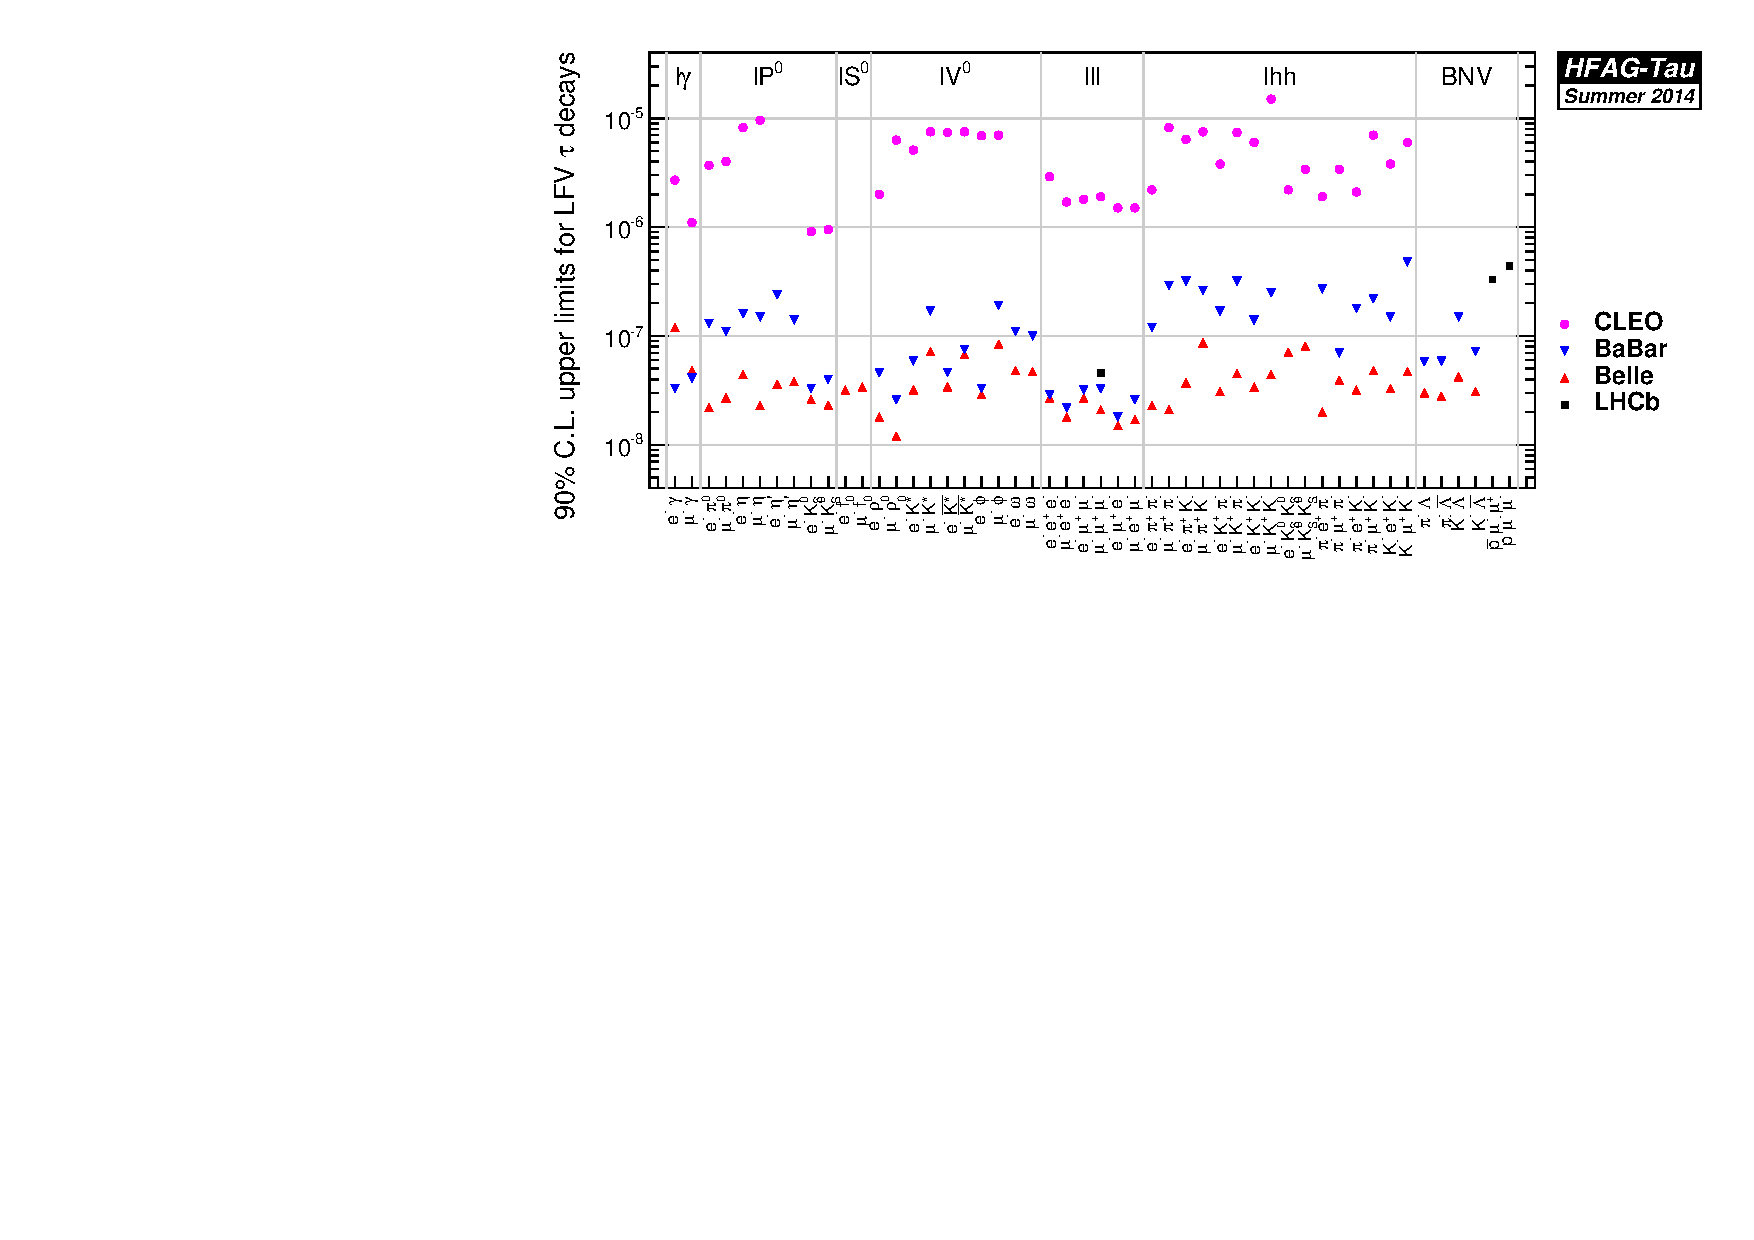
\includegraphics[angle=270,totalheight=0.9\textheight,clip]{figures/tau/TauLFV_UL_2014001.pdf}
    \fi
    \caption{Tau lepton-flavor-violating branching fraction upper
      limits summary plot.
      \label{fig:tau:lfv-limits-plot}
    }
  \end{center}
\end{figure}

%% -*- mode: LaTeX; TeX-master: "../EndOfYear11.tex" -*-
\tausection{Combination of Upper Limits on \mtau LFV Branching Fractions}
\cutname{lfv-limits-combinations.html}
\label{sec:tau:lfv_com}
\newcommand{\cls}{\ensuremath{CL_s}\xspace}

<<<<<<< .mine
There is no standard and generally agreed method of combining experimental upper
limits on branching fractions. The available results on \mtau LFV branching
fractions upper limits are determined with a variety of methods and there is
no straightforward way to combine the upper limits as quoted in the papers
acccordingly. We propose and implement in this section a combination of the
published upper limits that is based on the following procedure:
\begin{itemize}

\item
  a new 90\% confidence level upper limit is computed for each result using
  the \cls method \cite{Mistlberger:2012rs} with the published
  information on the observed events, the expected background, the signal
  efficiency, and the sample size;

\item
  the re-computed \cls limits are combined to provide the HFAG average.

\end{itemize}
The \cls method 

In this section we report on our combination of upper limits of tau LFV
branching fractions. We would like stress out that most of the searches
listed in~\ref{tab:tau:lfv-upper-limits} observed a downward
fluctuation. Since downward fluctuations in
Feldmann-Cousinus~\cite{PhysRevD.57.3873} can lead to artificial low
exclusions~\cite{PhysRevD.86.010001} on branching fractions we choose to
\cls \cite{Mistlberger:2012rs} method which alleviates this effect.

=======
In this section we report on our combination of upper limits of tau LFV branching fractions. We would like stress out that most of the searches listed in~\ref{tab:tau:lfv-upper-limits} observed a downward fluctuation. Since downward fluctuations in Feldmann-Cousinus~\cite{Feldman:1998} can lead to artificial low exclusions~\cite{PDG_2013} on branching fractions we choose to \cls \cite{Mistlberger:2012rs} method which alleviates this effect. \\
>>>>>>> .r1082
\cls method is based on two hypothesis: signal + background and background only. We calculate observed confidence levels for the two hypothesis:
\begin{align}
CL_{s+b} = P_{s+b}(Q \leq Q_{obs}) = \int_{- \infty}^{Q_{obs}} \frac{dP_{s+b}}{dQ} dQ,\\
CL_{b} = P_{b}(Q \leq Q_{obs}) = \int_{- \infty}^{Q_{obs}} \frac{dP_{b}}{dQ} dQ,
\label{pdfs}
\end{align}
where $CL_{s+b}$ is confidence level observed for signal + background hypothesis, $CL_{b}$ is confidence level observed for background only hypothesis, $\frac{dP_{s+b}}{dQ}$ and $\frac{dP_{b}}{dQ}$ are probability distribution functions (p.d.f.'s) for the two corresponding hypothesis and $Q$ is so called test statistics. \cls value is defined as normalized confidence level observed for signal plus background hypothesis to confidence level observed for background hypothesis:
\begin{equation}
CL_s=\dfrac{CL_{s+b}}{CL_{b}}.
\end{equation}\\
For multichannel searches the p.d.f.'s from~\ref{pdfs} become a product of individual p.d.f.'s for given experiment. One can write the \cls value explicit:
\begin{equation}
CL_s = \dfrac{\prod_{i=1}^{N_{chan}}\sum_{n=0}^{n_i} \dfrac{e^{-(s_i+b_i)} (s_i+b_i)^{n}}{n!} }{\prod_{i=1}^{n_{chan}}  \sum_{n=0}^{n_i} \dfrac{e^{-b_i} b_i^{n}}{n!}}    \dfrac{\prod_{j=1}^{n} s_iS_i(x_{ij})+b_iB_i(x_{ij})}{\prod_{j=1}^{n_i}B_i(x_{ij})},
\end{equation}
where $N_{chan}$ are number of channels, $n_i$ is the number of observed candidates in the $i^{th}$ channel, $x_{ij}$ are the values of discriminating variables, $s_i$ and $b_i$ are the number of signal and background events in the $i^{th}$ channel and $S_i$, $B_i$ are the probability distribution functions of the discriminating variables. \\
For the technical implementation we used an implementation provided by Tom Junk\cite{tjunk}. For each experiment we estimated the number of expected signal events using the formula:
\begin{equation}
\begin{split}
s_i & =2\mathcal{L}_i\sigma_{\tau\tau}Br(\tau \rightarrow LFV) \\
& =\frac{Br(\tau \rightarrow LFV)}{\alpha},
\end{split}
\end{equation}
where $\mathcal{L}_i$ is the integrated luminosity of an given experiment, $\sigma_{\tau\tau}$ is the cross section of a process $e^+ e^- \rightarrow  \tau^+ \tau^-$, $Br(\tau \rightarrow LFV)$ is the branching fraction of searched process and $\alpha$ is so called normalization factor\footnote{In case of LHCb results we take the the normalization directly from the appropriate paper.}. The systematics uncertainties are evaluated in pseudoexperiments generation by varying nuisance parameters($s_i$, $b_i$). The values are varied accordingly to Gaussian distribution width equal to corresponding systematic.\\
As mentioned at the begging most of the limits calculated by the B factories used Feldman-Cousin method, for comparison purposes in table~\ref{tab:tau:lfv-upper-limits_comb} we reported individual limits calculated with \cls method as well our combined limit. The same numbers are shown in Figure~\ref{fig:tau:lfv-limits-plot_average}. CLEO results were not taken into account because of negligible impact, also if a result between Belle an \babar is an order of magnitude stronger we did not perform a combination of this limits.



\begin{center}
\begin{longtable}{lcl@{}rl}

\caption{HFAG 2014  upper limit for the lepton flavor violating $\tau$ decay modes combinations. Individual experiments limits are recalculated using \cls method and final combination is reported. For convenience, the decay modes
are grouped in categories labelled according to their particle content. The label ``(L)'' in the category column means that the decay mode implies lepton number violation as well as the lepton flavor violation. ``BNV'' indicates that the channel is Baryon Number Violating.
\label{tab:tau:lfv-upper-limits_comb}}%
\\
\hline
\multicolumn{1}{l}{\bfseries Decay mode} &
\multicolumn{1}{l}{\bfseries Category} &
\multicolumn{2}{c}{\bfseries \begin{tabular}{@{}c@{}}90\% CL\\Limit\end{tabular}} &
\multicolumn{1}{l}{\bfseries Exp.}\\% &
%\multicolumn{1}{l}{\bfseries Ref.} \\
\hline
\endfirsthead
\multicolumn{5}{c}{{\bfseries \tablename\ \thetable{} -- continued from previous page}} \\ \hline
\multicolumn{1}{l}{\bfseries Decay mode} &
\multicolumn{1}{l}{\bfseries Category} &
\multicolumn{2}{c}{\bfseries \begin{tabular}{@{}c@{}}90\% CL\\Limit\end{tabular}} &
\multicolumn{1}{l}{\bfseries Exp.}\\% &
%\multicolumn{1}{l}{\bfseries Ref.} \\
\hline
\endhead
%
%  l\gamma
%   

\begin{ensuredisplaymath}
\Gamma_{156} =  {e^- \gamma} 
\end{ensuredisplaymath}
 &\(l\gamma\) & \( <\; \) &  \(5.4 \cdot 10^{-8}\)         & HFAG \\
 &            & \( <\; \) & \(22.0 \cdot 10^{-8}\)         & Belle \\
 &            & \( <\; \) & \(6.1 \cdot 10^{-8}\)         & \babar  \\ 
%\hline
\begin{ensuredisplaymath}
\Gamma_{157} =  {\mu^- \gamma} 
\end{ensuredisplaymath}
 &            & \( <\; \) &  \(5.0 \cdot 10^{-8}\)         & HFAG \\
 &            & \( <\; \) & \(17.0 \cdot 10^{-8}\)         & Belle  \\
 &            & \( <\; \) & \(5.9 \cdot 10^{-8}\)         & \babar   \\ 
\hline
%
%  lP0
\begin{ensuredisplaymath}
\Gamma_{160} =  {e^- K^0_S} 
\end{ensuredisplaymath}
 & \(lP^0 \)  & \( <\; \) & \(1.4 \cdot 10^{-8}\)         & HFAG  \\
 &            & \( <\; \) & \(1.8 \cdot 10^{-8}\)         & Belle  \\
 &            & \( <\; \) & \(4.7 \cdot 10^{-8}\)         & \babar   \\ 
%\hline
\begin{ensuredisplaymath}
\Gamma_{161} =  {\mu^- K^0_S} 
\end{ensuredisplaymath}
 &            & \( <\; \) & \(1.5 \cdot 10^{-8}\)         & HFAG  \\
&            & \( <\; \) & \(1.7 \cdot 10^{-8}\)         & Belle  \\
 &            & \( <\; \) & \(6.9 \cdot 10^{-8}\)         & \babar   \\ 
\hline
%
% l V0
%
\begin{ensuredisplaymath}
\Gamma_{164} =  {e^- \rho^0} 
\end{ensuredisplaymath}
 &  \(l V^0\) & \( <\; \) & \(1.5 \cdot 10^{-8}\)         & HFAG  \\
 &            & \( <\; \) & \(1.9 \cdot 10^{-8}\)         & Belle\\
 &            & \( <\; \) & \(5.2 \cdot 10^{-8}\)         & \babar   \\ 
%\hline
\begin{ensuredisplaymath}
\Gamma_{165} =  {\mu^- \rho^0} 
\end{ensuredisplaymath}
 &            & \( <\; \) & \(1.5 \cdot 10^{-8}\)         & HFAG  \\
 &            & \( <\; \) & \(2.1 \cdot 10^{-8}\)         & Belle\\
 &            & \( <\; \) & \(6.2 \cdot 10^{-8}\)         & \babar \\ 
%\hline
\begin{ensuredisplaymath}
\Gamma_{168} =  {e^- K^*(892)^0} 
\end{ensuredisplaymath}
 &            & \( <\; \) & \(2.3 \cdot 10^{-8}\)         & HFAG \\
 &            & \( <\; \) & \(3.4 \cdot 10^{-8}\)         & Belle \\
 &            & \( <\; \) & \(6.1 \cdot 10^{-8}\)         & \babar   \\ 
%\hline
\begin{ensuredisplaymath}
\Gamma_{169} =  {\mu^- K^*(892)^0} 
\end{ensuredisplaymath}
 &            & \( <\; \) & \(6.0 \cdot 10^{-8}\)         & HFAG \\
 &            & \( <\; \) & \(6.6 \cdot 10^{-8}\)         & Belle \\
 &            & \( <\; \) & \(17.0 \cdot 10^{-8}\)         & \babar   \\ 
%\hline
\begin{ensuredisplaymath}
\Gamma_{170} =  {e^- \bar{K}^*(892)^0} 
\end{ensuredisplaymath}
 &            & \( <\; \) & \(2.2 \cdot 10^{-8}\)         & HFAG \\
 &            & \( <\; \) & \(3.3 \cdot 10^{-8}\)         & Belle \\
 &            & \( <\; \) & \(5.6 \cdot 10^{-8}\)         & \babar   \\ 
%\hline
\begin{ensuredisplaymath}
\Gamma_{171} =  {\mu^- \bar{K}^*(892)^0} 
\end{ensuredisplaymath}
 &            & \( <\; \) & \(4.2 \cdot 10^{-8}\)         & HFAG  \\
 &            & \( <\; \) & \(6.3 \cdot 10^{-8}\)         & Belle  \\
 &            & \( <\; \) & \(9.1 \cdot 10^{-8}\)         & \babar \\ 
%\hline

\begin{ensuredisplaymath}
\Gamma_{176} =  {e^- \phi} 
\end{ensuredisplaymath}
 &            & \( <\; \) & \(2.0 \cdot 10^{-8}\)         & HFAG \\
 &            & \( <\; \) & \(3.5 \cdot 10^{-8}\)         & Belle \\
 &            & \( <\; \) & \(4.3 \cdot 10^{-8}\)         & \babar   \\ 
%\hline
\begin{ensuredisplaymath}
\Gamma_{177} =  {\mu^- \phi} 
\end{ensuredisplaymath}
 &            & \( <\; \) &\(6.8 \cdot 10^{-8}\)         & HFAG \\
 &            & \( <\; \) &\(7.6 \cdot 10^{-8}\)         & Belle  \\
 &            & \( <\; \) & \(18.0 \cdot 10^{-8}\)         & \babar   \\ 
%\hline
\begin{ensuredisplaymath}
\Gamma_{166} =  {e^- \omega} 
\end{ensuredisplaymath}
 &            & \( <\; \) & \(3.3 \cdot 10^{-8}\)         & HFAG \\
 &            & \( <\; \) & \(5.2 \cdot 10^{-8}\)         & Belle  \\
 &            & \( <\; \) & \(9.4 \cdot 10^{-8}\)         & \babar    \\ 
%\hline
\begin{ensuredisplaymath}
\Gamma_{167} =  {\mu^- \omega} 
\end{ensuredisplaymath}
 &            & \( <\; \) & \(4.0 \cdot 10^{-8}\)         & HFAG \\
 &            & \( <\; \) & \(6.1 \cdot 10^{-8}\)         & Belle  \\
 &            & \( <\; \) &  \(10.0 \cdot 10^{-8}\)         & \babar   \\ 
\hline
%
% lll
%
\begin{ensuredisplaymath}
\Gamma_{178} =  {e^- e^+ e^-} 
\end{ensuredisplaymath}
 &  \(lll\)   & \( <\; \) & \(1.4 \cdot 10^{-8}\)         & HFAG \\
 &            & \( <\; \) & \(2.7 \cdot 10^{-8}\)         & Belle  \\
 &            & \( <\; \) & \(3.1 \cdot 10^{-8}\)         & \babar    \\ 
%\hline
\begin{ensuredisplaymath}
\Gamma_{181} =  {\mu^- e^+ e^-} 
\end{ensuredisplaymath}
 &            & \( <\; \) & \(1.1 \cdot 10^{-8}\)         & HFAG \\
 &            & \( <\; \) & \(1.7 \cdot 10^{-8}\)         & Belle \\
 &            & \( <\; \) & \(3.0 \cdot 10^{-8}\)         & \babar    \\ 
%\hline
\begin{ensuredisplaymath}
\Gamma_{179} =  {e^- \mu^+ \mu^-} 
\end{ensuredisplaymath}
 &            & \( <\; \) & \(1.6 \cdot 10^{-8}\)         & HFAG \\
 &            & \( <\; \) & \(2.6 \cdot 10^{-8}\)         & Belle  \\
 &            & \( <\; \) & \(4.1 \cdot 10^{-8}\)         & \babar     \\ 
%\hline
\begin{ensuredisplaymath}
\Gamma_{183} =  {\mu^- \mu^+ \mu^-} 
\end{ensuredisplaymath}
 &            & \( <\; \) & \(1.2 \cdot 10^{-8}\)         & HFAG \\
 &            & \( <\; \) & \(2.1 \cdot 10^{-8}\)         & Belle\\
 &            & \( <\; \) & \(4.0 \cdot 10^{-8}\)         & \babar  \\ 
 &            & \( <\; \) & \(4.6 \cdot 10^{-8}\)         & \lhcb   \\ 

%\hline
\begin{ensuredisplaymath}
\Gamma_{182} =  {e^- \mu^+ e^-} 
\end{ensuredisplaymath}
 &            & \( <\; \) & \(8.4 \cdot 10^{-9}\)         & HFAG \\
 &            & \( <\; \) & \(1.4 \cdot 10^{-8}\)         & Belle  \\
 &            & \( <\; \) & \(2.1 \cdot 10^{-8}\)         & \babar    \\ 
%\hline
\begin{ensuredisplaymath}
\Gamma_{180} =  {\mu^- e^+ \mu^-} 
\end{ensuredisplaymath}
 &            & \( <\; \) & \(9.8 \cdot 10^{-9}\)         & HFAG \\
 &            & \( <\; \) & \(1.6 \cdot 10^{-8}\)         & Belle \\
 &            & \( <\; \) & \(2.6 \cdot 10^{-8}\)         & \babar     \\ 
 %
% Lambda h
%
\hline
\begin{ensuredisplaymath}
\Gamma_{211} =  { \pi^- \Lambda } 
\end{ensuredisplaymath}
& BNV & \( <\; \) & \(1.9 \cdot 10^{-8}\)         & HFAG  \\
&                & \( <\; \) & \(3.2 \cdot 10^{-8}\)         & Belle  \\
 &               & \( <\; \) & \(6.7 \cdot 10^{-8}\)        & \babar     \\  
%\hline
\begin{ensuredisplaymath}
\Gamma_{212} =  { \pi^- \bar{\Lambda}} 
\end{ensuredisplaymath}
 &            & \( <\; \) & \(1.8 \cdot 10^{-9}\)         & HFAG \\
 &            & \( <\; \) & \(2.9 \cdot 10^{-8}\)         & Belle  \\
 &            & \( <\; \) & \(6.5 \cdot 10^{-8}\)        & \babar     \\  
%\hline
\begin{ensuredisplaymath}
\Gamma_{213} =  { K^- \Lambda } 
\end{ensuredisplaymath}
 &            & \( <\; \) & \(3.7 \cdot 10^{-9}\)         & HFAG \\
 &            & \( <\; \) & \(4.4 \cdot 10^{-8}\)         & Belle  \\
 &            & \( <\; \) & \(9.2\cdot 10^{-8}\)         & \babar     \\  
%\hline
\begin{ensuredisplaymath}
\Gamma_{214} =  { K^- \bar{\Lambda}} 
\end{ensuredisplaymath}
 &            & \( <\; \) & \(2.0 \cdot 10^{-9}\)         & HFAG \\
 &            & \( <\; \) & \(3.4 \cdot 10^{-8}\)         & Belle \\
 &            & \( <\; \) & \(5.0 \cdot 10^{-8}\)         & \babar     \\  
\hline 
\end{longtable}
\end{center}

%% -*- mode: LaTeX; TeX-master: "../Summer14.tex" -*-
%% ///////////////////////////////////////////////////////////////////////////
\ifhevea
\tausection{Combination of Upper Limits on \mtau LFV Branching Fractions: Summary Plot}
\cutname{lfv-combinations-plot.html}
\fi

\begin{figure}[tb]
  \begin{center}
    \ifhevea
    \begin{tabular}{@{}cc@{}}
      \larger\bfseries\ahref{TauLFV_UL_2014001_averaged.png}{full size PNG} &
      \larger\bfseries\ahref{TauLFV_UL_2014001_averaged.pdf}{PDF format} \\
      \multicolumn{2}{c}{\ahref{TauLFV_UL_2014001_averaged.png}{%
          \imgsrc[alt="Tau LFV limits combinations plot" width=720]{TauLFV_UL_2014001_averaged.png}}}
    \end{tabular}
    \else
    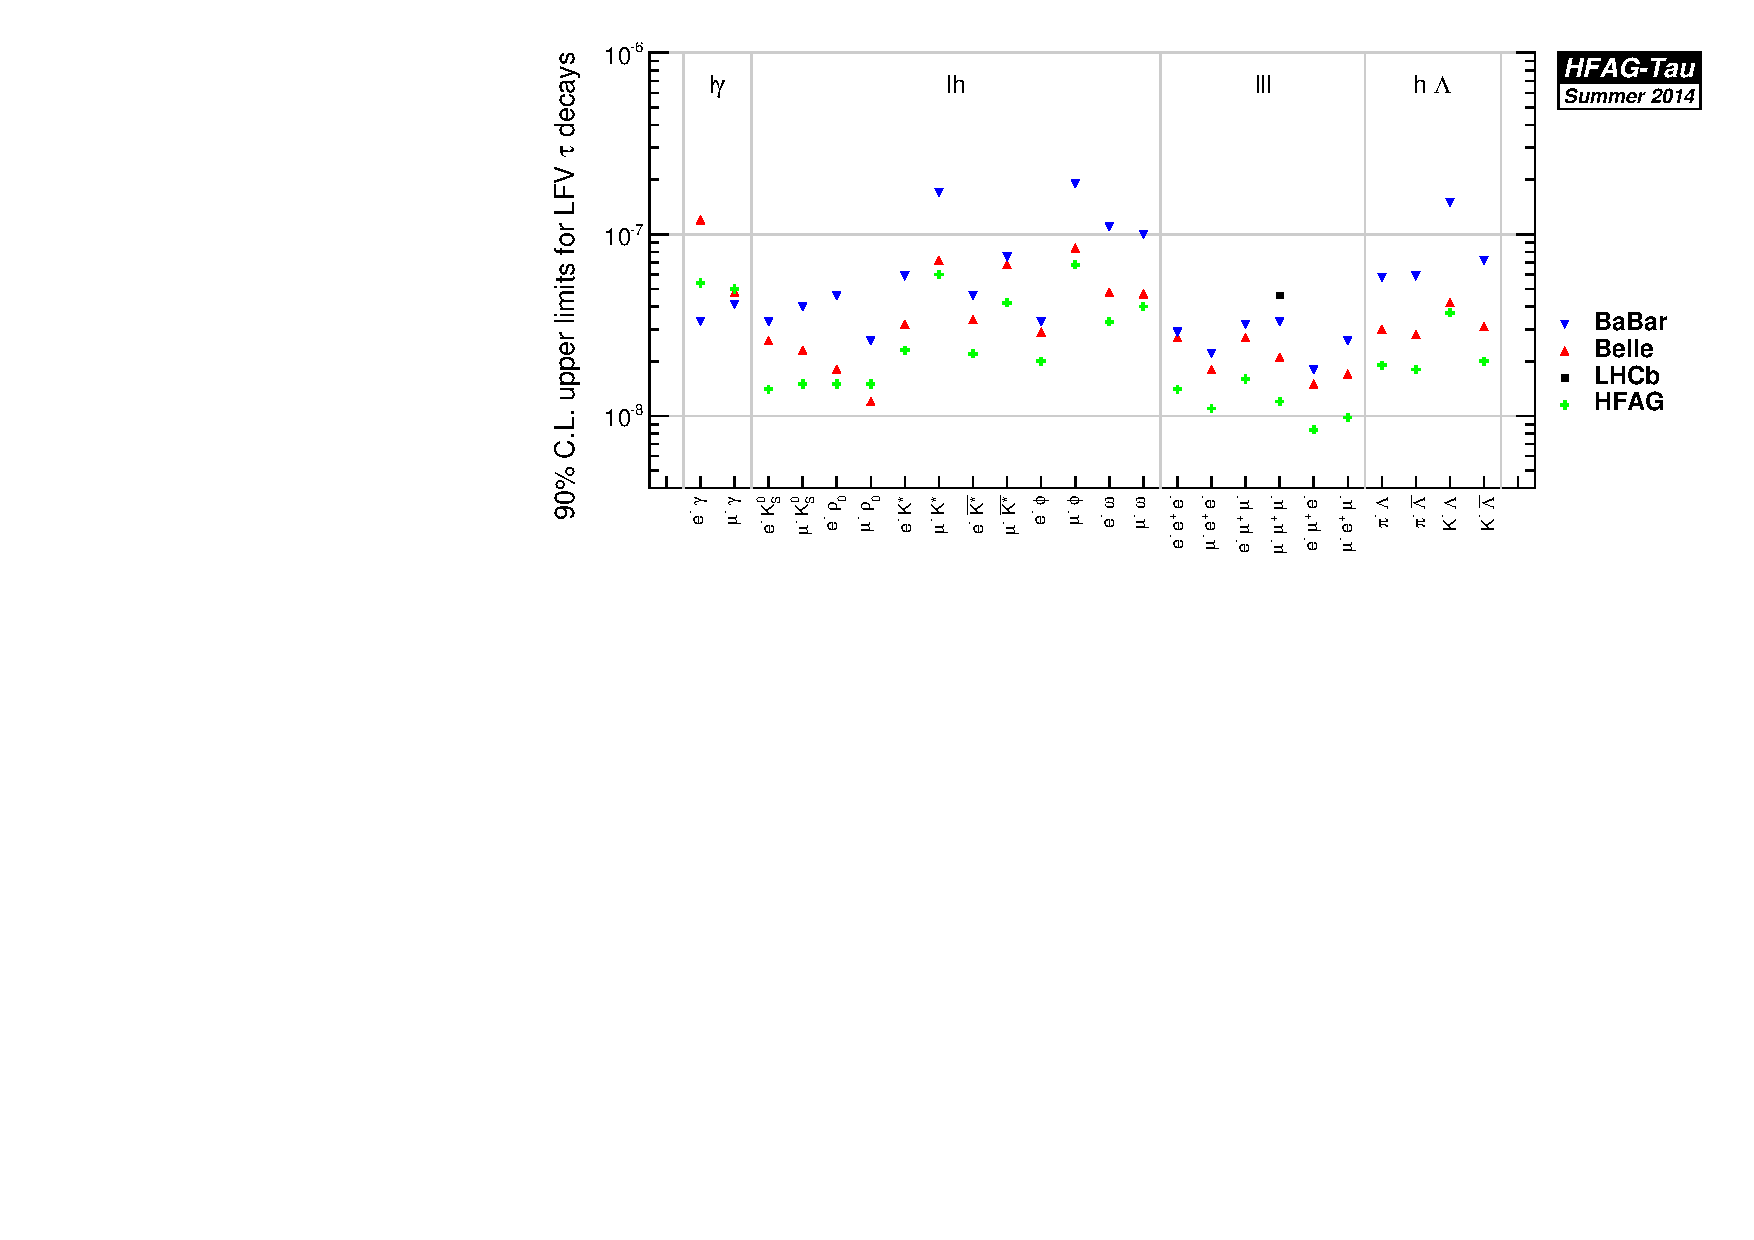
\includegraphics[angle=270,totalheight=0.9\textheight,clip]{figures/tau/TauLFV_UL_2014001_averaged}
    \fi
    \caption{Tau lepton-flavour-violating branching fraction upper limits combinations summary plot.
      \label{fig:tau:lfv-limits-plot_average}
    }
  \end{center}
\end{figure}

\let\tausection\subsection
%%--- end
\let\cite\citeOld
\end{fleqn}
